\documentclass[a4paper, 11pt, twoside, openright, italian]{memoir}

\usepackage{preamble/mypreamble}


% SVN info for this file
\svnidlong
{$HeadURL$}
{$LastChangedDate$}
{$LastChangedRevision$}
{$LastChangedBy$}

\includeonly{%
  introduction/titlepage,
  introduction/introduction,
  introduction/toc,
  chapters/chap1,
  chapters/chap2,
  chapters/chap3,
  chapters/chap4,
  chapters/chap5,
  chapters/chap6,
  chapters/chap7,
  chapters/chap8,
  chapters/chap9,
  %chapters/chap10,
  %chapters/chap11,
  %chapters/chap12,
  appendix/footnotes,
  appendix/settheory,
  %appendix/prop,
  appendix/list,
  appendix/ringraziaments,  
  appendix/bibliography,
}

\makeindex
\begin{document}

\frontmatter
% SVN info for this file
\svnidlong
{$HeadURL$}
{$LastChangedDate$}
{$LastChangedRevision$}
{$LastChangedBy$}

% Remove header and footer
\thispagestyle{empty}
\addtocounter{page}{-1}

\begin{textblock}{1}(0,0)
	\noindent\textcolor{blueill}{\rule{\paperwidth}{.55\paperheight}}
\end{textblock}


\begin{textblock}{1}(0,.55)
	\noindent\textcolor{black}{\rule{\paperwidth}{.45\paperheight}}
\end{textblock}


\begin{textblock}{1}(.00,.11)
	%\begin{center}
	%\noindent{\fontsize{39.88}{2}\selectfont
	%	\bfseries\textcolor{white}{\textsc{FATTO DI SANGUE\\[4.5mm]TRA DUE ANALISTI\\[4.5mm]PER CAUSA DI UN\\[4.5mm]INTEGRALE}}}
	%\end{center}
\end{textblock}

\begin{textblock}{1}(.00,.31)
	%\begin{center}
	%\noindent {\fontsize{24.88}{2}\selectfont
	%	\bfseries\textcolor{white}{\textsc{Si sospettano moventi misurabili}}}
	%\end{center}
\end{textblock}

% \begin{textblock}{1}(.1,.21)
%     \noindent{\fontsize{30}{2}\selectfont
%         \bfseries\textcolor{white}{for \LaTeX}}
% \end{textblock}

\begin{textblock}{1}(.00,.06)
	\begin{center}
	
\includegraphics[width=0.8\paperwidth]{images/uncompressed/titolo}
	%		\noindent {\fontsize{20.74}{2}\selectfont
	%		\bfseries\textcolor{white}{Elisa Antuca\ \ \ Massimo Bertolotti}}
	\end{center}
\end{textblock}



\begin{textblock}{.9}(.05,.56)
	\begin{flushright}
		\noindent {\fontsize{20.74}{2}\selectfont
			\bfseries\textcolor{white}{Manualozzo di Analisi Matematica 3}}
	\end{flushright}
\end{textblock}


\begin{textblock}{.45}(.55,.705)
	\begin{center}
		
\includegraphics[width=.35	\paperwidth]{images/copertina2}
	\end{center}
\end{textblock}

\begin{textblock}{.1}(-.005,.59)
	\begin{center}
		
\includegraphics[width=.38\paperwidth]{images/copertina3}
	\end{center}
\end{textblock}

\begin{textblock}{.4}(.3,.35)
	\begin{center}
		
\includegraphics[width=.2\paperwidth]{images/unitologo}
	\end{center}
\end{textblock}

\begin{textblock}{.6}(.1,.58)
	\noindent {\fontsize{14.74}{18}%
		\textcolor{white}{$\displaystyle\lambda=\limsup_{n\to+\infty}\sqrt[n]{\abs{n}}$}}
\end{textblock}


\begin{textblock}{.3}(.245,.86)
	\noindent {\fontsize{15.28}{18}%
		\textcolor{white!80}{$\displaystyle\lim_{n\to+\infty}\int_Xf_nd\mu=\int_X\lim_{n\to+\infty}f_nd\mu$}}
\end{textblock}

\begin{textblock}{.4}(.05,.91)
	\noindent {\fontsize{14.4}{18}%
		\textcolor{white!50}{$\displaystyle \mu\left(\bigcup_{n\geq 1}A_n\right)=\lim_{n\to+\infty}\mu\left(A_n\right)$}}
\end{textblock}

\begin{textblock}{.6}(.36,.605)
	\begin{center}
		
\includegraphics[width=.575\paperwidth]{images/copertina1}
	\end{center}
\end{textblock}


\begin{textblock}{.3}(.395,.75)
	\noindent {\fontsize{18.28}{18}%
		\textcolor{white!10}{$\displaystyle e^z\coloneqq \sum_{n=0}^{+\infty}\frac{z^n}{n!}$}}
\end{textblock}



\null\newpage
\begin{comment}
	\begin{center}
	\newlength{\parSepLength}
	\setlength{\parSepLength}{10ex}
	
	\Large
	\centering
	
	% Main title
	\thinRule\par
	\par\vspace{0.15\parSepLength}
	\begin{minipage}{\textwidth}
	\centering
	\fontsize{40pt}{36pt}\selectfont\titleColor\scshape
	Appunti di Geometria 2
	\end{minipage}
	\par\vspace{0.25\parSepLength}
	\par\thinRule
	
	\vspace{0.125\parSepLength}
	
	\begin{minipage}{\textwidth}
	\centering
	\small
	Anno Accademico 2020/2021
	\end{minipage}
	
	\vspace{0.225\parSepLength}
	
	\begin{minipage}{\textwidth}
	\centering
	‘‘Un matematico è una macchina per trasformare caffè in teoremi.''\\
	Alfréd Rényi
	\end{minipage}
	
	\vfill
	
	% Author
	\begin{minipage}{\textwidth}
	\centering
	%\Large
	\begin{center}
	\includegraphics[width=0.25\linewidth]{images/Unito-logo}
	\end{center}
	
	\end{minipage}
	
	\vfill
	
	% Logo and other info
	% \begin{minipage}{0.8\textwidth}
	%    \centering
	%    \small
	
	% Examiner
	%    \begin{minipage}[t]{0.29\textwidth}
	%      \textsc{Titolari del corso} \\
	%     {\scriptsize Prof. Marco Costa\\
	%      Prof. Antonaldo Diaferio\\
	%       Università di Torino}
	%    \end{minipage}
	%   \hfill
	% Supervisor
	%   \begin{minipage}[t]{0.26\textwidth}
	%      \begin{center}
	%     	\textsc{Adattamento \LaTeX} \\ 
	%     \textsc{e integrazioni discutibili} \\
	%     {\scriptsize Massimo Bertolotti\\
	%      Università di Torino}
	%     \end{center}
	%   \end{minipage}
	%	\hfill
	%	\begin{minipage}[t]{0.27\textwidth}
	%	\raggedleft
	%	\textsc{Revisione contenutistica} \\ 
	%	{\scriptsize Elisa Antuca\\
	%	 Università di Torino}
	%	\end{minipage}
	%  \end{minipage}
	\end{center}
\end{comment}
\afterpage{\blankpage}
% SVN info for this file
\svnidlong
{$HeadURL$}
{$LastChangedDate$}
{$LastChangedRevision$}
{$LastChangedBy$}

\chapter*{Introduzione al Manualozzo}
\labelChapter{introduzione}

\begin{introduction}
‘‘Sai, per essere un matematico non aveva abbastanza immaginazione; ma ora è diventato un poeta e se la cava davvero bene.''
\begin{flushright}
	\textsc{David Hilbert,} riferendosi \Ccancel[red]{a Marino Badiale} all'autore del Manualozzo.
\end{flushright}
\end{introduction}

\noindent Guardando la copertina di questo testo, dei potenziali lettori - sì, parlo con voi - si potrebbero chiedere: ‘‘Ma che diamine è un \textit{manualozzo}?''
\vspace{3mm}
\lettrine[findent=1pt, nindent=0pt]{\textbf{M}}{\textbf{anualozzo}} s. m. [der. di \textit{manuale}, col suff. \textit{-ozzo}]. - Appunti di lezioni universitarie scritti da studenti, scritti senza troppe pretese di formalità e potenzialmente non totalmente corretti, ma sono comunque meglio che niente.
\vspace{3mm}\\
Dunque, quello che state leggendo è il \textbf{Manualozzo di Analisi Matematica 3}, basato sull'omonimo corso tenuto dai docenti Walter Dambrosio e Davide Zucco nell'a.a. 2021-2022 presso il Dipartimento di Matematica dell'Università degli Studi di Torino.\\
L'insegnamento - e di conseguenza questo testo - si articola in due macro-temi strettamente correlati tra di loro: lo studio delle \textbf{successioni} e delle \textbf{serie di funzioni} e la trattazione della \textbf{teoria della misura} e dell'\textbf{integrazione (secondo Lebesgue)}. I prerequisiti necessari sono gli argomenti trattati nel corso di \textsc{Analisi Matematica Uno} - ma non fa male avere anche qualche nozione da \textsc{Calcolo delle Probabilità}.\\
Ma il \textit{Manualozzo} non è una mera sbobinatura delle lezioni: in aggiunta agli argomenti trattati nella teoria, potrete trovare a fine libro delle utili \textit{postille} con alcune digressioni interessanti, nonché tabelle ed elenchi riepilogativi dei teoremi, delle definizioni e delle proprietà affrontate - il tutto, ovviamente, in Technicolor\textsuperscript{TM}.\\
Purtroppo, per quanto gli piacerebbe esserlo, l'autore non è un \textit{essere infallibile}: gli saranno sicuramente sfuggiti degli errori (o degli \textit{orrori}, la cui causa è solamente dall'autore che non ha studiato bene e non dei professori, chiaramente), per cui ogni segnalazione - direttamente all'autore se ancora in vita oppure su \textcolor{redill}{\url{https://maxmaci.github.io}} - è ben gradita, in modo da migliorare le future edizioni del \textit{Manualozzo}.\\

\vfill
\begin{center}
	Prima edizione, compilato il \today.\\
			
\includegraphics[trim=0cm 0cm 0cm 0cm,clip,scale=0.5]{images/Cc-by-nc-sa_icon.pdf}\\
	{\footnotesize This work is licensed under a \href{https://creativecommons.org/licenses/by-sa/4.0/}{Attribution-NonCommercial-ShareAlike 4.0 International.}}
\end{center}
\newpage
\section*{Note per gli environment}
Se alcuni professori sono noti per abusare le notazioni, i Manualozzi sono noti per abusare di \textit{environment} - gli ambienti colorati che vedrete in queste pagine; di seguito ci sono alcune informazioni su di essi.

\noindent\textit{Teoremi}, \textit{proposizioni}, \textit{lemmi} e \textit{corollari} possono essere seguiti da una \textit{dimostrazione}, come nell'esempio di seguito...
\begin{theoremanote}[Tete numquam relinquam]
	Amoris sumus periti, leges noscis necnon ego; devotionem plenam intendo, hanc non habebis ex ullo alio.
\end{theoremanote}
\begin{demonstration}
	Communicare volo tibi quod sentio - intelligendum tibi est.
\end{demonstration}
... oppure essere forniti \textit{senza} dimostrazione e quindi nell'enunciato troverete alla fine il simbolo $\square$:
\begin{corollarynote}[Ricardovolvere]
	Tete numquam relinquam, tete numquam deseram - tibi ero desultor non numquam; faciam non flere te, nec dicam valere,
	mendax vulnerabo non numquam.
\end{corollarynote}
Nelle sezioni ‘‘Eserciziamoci!'' potrete invece trovare esercizi con corrispettive soluzioni: sono simili talvolta a dei risultati teorici, ma tendono ad essere più applicativi.

\noindent Alcuni degli \textit{environment} più comuni dopo questi sono le \textit{osservazioni} e gli \textit{esempi}, che sono autoesplicativi. Ci sono anche altri \textit{environment}, meno comuni, fra cui...
\begin{digression}
	Sono argomenti \textit{non prettamente trattati} in questo corso che, tuttavia, hanno un legame con esso: possono \textit{aggiungere informazioni} e punti di vista a qualcosa visto nei corsi precedenti oppure fornire delle \textit{anticipazioni} per dei corsi futuri.
\end{digression}
\begin{attention}
	Sono delle osservazioni mirate e rivolte spesso a segnalare \textit{errori} frequenti, dovuti principalmente a proprietà che \textit{non} si verificano in quel dato tangente. 
\end{attention}
\begin{intuit}
	Sono delle interpretazioni \textit{euristiche} di una definizione difficile o di un risultato ostico che possono aiutare a capire il perché di tale cosa - per quanto formalmente non sia sempre valide a livello formale. 
\end{intuit}
\section*{Note per gli elenchi delle definizioni e dei teoremi}
In fondo al Manualozzo si possono trovare degli elenchi con tutte le definizioni, assiomi e risultati teorici visti: ognuno di essi è indicato nel formato \textbf{\textsc{X\#.\#.\#. TITOLO}}, dove \textbf{\textsc{X}} indica una \textit{sigla} per indicare il tipo di definizione/risultato, mentre \textbf{\textsc{\#.\#.\#.}} individua il \textit{capitolo}, la \textit{sezione} e il \textit{numero} per quell'oggetto nella sezione. I significati delle sigle è sono elencati di seguito:
\begin{itemize}
	\item \textbf{\textsc{A}}: Assioma
	\item \textbf{\textsc{D}}: Definizione
	\item \textbf{\textsc{T}}: Teorema
	\item \textbf{\textsc{PR}}: Proposizione
	\item \textbf{\textsc{L}}: Lemma
	\item \textbf{\textsc{C}}: Corollario
	\item \textbf{\textsc{PT}}: Proprietà
\end{itemize}


% SVN info for this file
\svnidlong
{$HeadURL$}
{$LastChangedDate$}
{$LastChangedRevision$}
{$LastChangedBy$}

\tableofcontents

\mainmatter

\part{Introduzione ad \textsc{Analisi Matematica 3}}
\labelPart{intro}
% SVN info for this file
\svnidlong
{$HeadURL$}
{$LastChangedDate$}
{$LastChangedRevision$}
{$LastChangedBy$}

\chapter{Alla ricerca della lunghezza dell'ellisse}
\labelChapter{ellipseintroduction}

\begin{introduction}
‘‘BEEP BOOP QUESTA È UNA CITAZIONE.''
\begin{flushright}
	\textsc{Marinobot,} dopo aver finito le citazioni stupide.
\end{flushright}
\end{introduction}
\lettrine[findent=1pt, nindent=0pt]{U}{na circonferenza} e un'\emph{ellisse} a primo acchito possono sembrare molto simili: in fondo, una circonferenza non è altro che un'ellisse i cui punti focali coincidono e dunque l'ellisse si può vedere come una circonferenza ‘‘allungata'' rispetto ad un asse. Il valore dell'area delimitata da una circonferenza ($\pi r^2$) e la lunghezza di una circonferenza ($2\pi r$) sono ben noti già dall'antichità, i cui calcoli sono stati opportunamente formalizzati in epoca moderna; tuttavia, riguardo l'ellisse, ci accorgiamo di aver incontrato nel corso degli studi precedenti quasi esclusivamente il valore dell'area delimitata da essa ($\pi ab$), ma \emph{non la lunghezza dell'ellisse}. Come mai?\\
\section{Una domanda banale: la lunghezza di un'ellisse}
Partiamo col seguente \textit{quiz}: quale delle seguenti tre espressioni è il valore, o una sua \textit{approssimazione}, della lunghezza di un'ellisse di semiassi di lunghezza $a$ e $b$?
\begin{enumerate}[label=\alph*)]
	\item $L\left(a,b\right)=\pi ab$
	\item $L\left(a,b\right)\approx \pi \left(a+b\right)+3\pi\frac{\left(a-b\right)^2}{10\left(a+b\right)+\sqrt{a^2+14ab+b^2}}$
	\item $L\left(a,b\right)\approx 2\pi a$.
\end{enumerate}
Chiaramente, come abbiamo detto nell'introduzione del capitolo, la lunghezza dell'ellisse \textit{non} è una formula nota dagli studi passati e possiamo (per ora) solamente escludere la \textit{prima risposta}, in quanto essa è il valore dell'\textbf{area} delimitata dell'ellisse.
\begin{observe}
	  Possiamo escludere la prima risposta anche per motivi puramente \textbf{dimensionali}: $a$ e $b$ sono, dimensionalmente parlando, due lunghezze, quindi $\pi ab$ deve essere una \textit{lunghezza al quadrato}, cioè un'area e non può essere una lunghezza!
\end{observe}
In realtà, la domanda del quiz è mal posta: le risposte \textit{b)} e \textit{c)} sono entrambe corrette.\\
Il matematico indiano Srinivasa Aiyangar Ramanujan fornì come nota a margine non commentata in un suo articolo del 1914 (\cite{ramanujan:1914piapprox}) l'approssimazione \textit{b)}:
\begin{equation*}
	L\left(a,b\right)\approx \pi\left(\left(a+b\right)+3\frac{\left(a-b\right)^2}{10\left(a+b\right)+\sqrt{a^2+14ab+b^2}}\right)
\end{equation*}
Vedremo fra poco che anche l'approssimazione data dalla \textit{a)} è anch'essa lecita.\\
Il motivo per cui diamo approssimazioni ma non formule esatte per la lunghezza dell'ellisse è dovuto al fatto che \textit{non esiste} una formula esplicita in termini di \textit{funzioni elementari}, bensì possiamo esprimerla soltanto come \textbf{somma di una serie}.
\begin{theorema}[Lunghezza dell'ellisse di semiassi di lunghezza $a$ e $b$.]~{}\\
	Siano $a\geq b$ le lunghezze dei semiassi dell'ellisse e $e=e\left(a,b\right)=\frac{\sqrt{a^2-b^2}}{a}\in\left[0,1\right)$ l'\textbf{eccentricità}\index{eccentricità}; allora si ha
	\begin{equation}
		L\left(a,b\right)=2\pi a\sum_{j=0}^{+\infty}\frac{1}{1-2j}\left(\frac{\left(2j-1\right)!!}{\left(2j\right)!!}e^j\right)^2
	\end{equation}
dove $!!$ indica il \textbf{doppio fattoriale}\index{fattoriale!doppio}:
\begin{itemize}
	\item $\left(-1\right)!!=0!!=1$
	\item $\forall n\in\naturalset\quad n!!=\begin{cases}
		n\cdot \left(n-2\right)\cdot \ldots \cdot 6 \cdot 4 \cdot 4 \cdot 2\text{ se }n>0\text{ è pari}\\
		n\cdot \left(n-2\right)\cdot \ldots \cdot 5 \cdot 3 \cdot 2 \cdot 1\text{ se }n>0\text{ è dispari}\\
	\end{cases}$
\end{itemize}
\end{theorema}
Il primo termine della serie fornisce l'approssimazione espressa nella risposta \textit{a)}:
\begin{equation*}
	L\left(a,b\right)\approx 2\pi a
\end{equation*}
\subsection{La problematica dimostrazione della lunghezza dell'ellisse: la serie di Taylor}
\begin{minipage}{0.49\textwidth}
	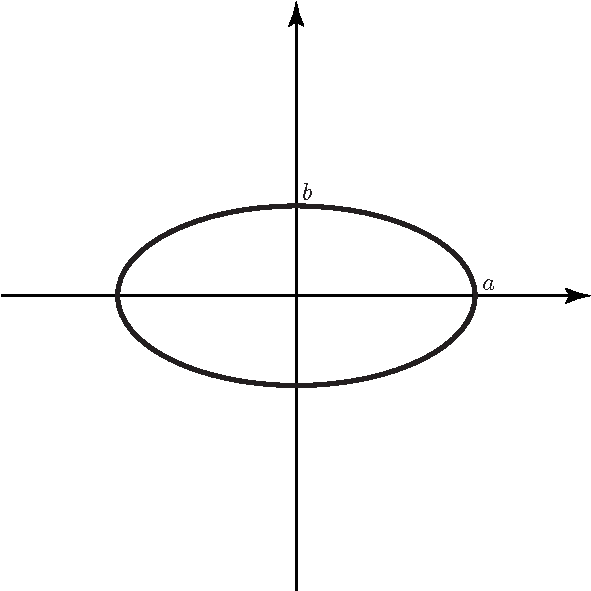
\includegraphics[trim=0cm 2.25cm 0cm 0cm, clip, scale=0.65]{images/ellisse.pdf}
\end{minipage}\hspace{-2mm}
\begin{minipage}{0.50\textwidth}
Dimostriamo finalmente la lunghezza dell'ellisse. Come è noto dal corso di \textsc{Analisi 2}, per una curva \textit{regolare} come l'ellisse è possibile calcolarne la lunghezza usando un'opportuna parametrizzazione.\\
Poniamo $a\geq b$ le lunghezze dei semiassi ed $e=\frac{\sqrt{a^2-b^2}}{a}\in\left[0,1\right)$ l'eccentricità. Una parametrizzazione è
\begin{equation*}
	\vec{r}\left(t\right)=\left(a\sin t,\ b\cos t\right)\quad t\in\left[0, 2\pi\right]
\end{equation*}
\end{minipage}\\
Allora
\begin{align*}
		L&=\int_{0}^{2\pi}\norm{\vec{r}'\left(t\right)}dt=\int_{0}^{2\pi}\norm{\left(a\cos t,\ -b\sin t\right)}dt=\int_{0}^{2\pi}\sqrt{a^2\cos^2t+b^2\sin^2t}dt=\\
		&=\int_{0}^{2\pi}\sqrt{a^2-\left(a^2+b^2\right)\sin^2t}dt=a\int_{0}^{2\pi}\sqrt{1-e^2\sin^2t}
\end{align*}
C'è un problema: la funzione $f\left(t\right)=\sqrt{1-e^2\sin^2t}$ non è \textbf{elementarmente integrabile}, cioè non ammette primitive in termini di funzioni elementari.
\begin{attention}
	Non essere elementarmente integrabile \textit{non} significa che non sia integrabile! La funzione integranda $f\left(t\right)$ è continua su $\left[0, 2\pi\right]$, dunque per il \textit{teorema fondamentale del calcolo integrale} ammette primitive su $\left[0, 2\pi\right]$. Una di esse è
	\begin{equation*}
		F\left(t\right)=\int_{0}^{t}\sqrt{1-e^2\sin^2y}dy\quad\forall y\in\left[0,2\pi\right]
	\end{equation*}
	Il problema è che \textit{non} possiamo riscrivere $F$ in modo esplicito usando \textit{solo} funzioni elementari.
\end{attention}
Questo tipo di integrale è detto \textbf{integrale ellittico}\index{integrale!ellittico}.
\begin{digression}
	Gli \textit{integrali ellittici} si incontrano in molti ambiti matematici. Ad esempio, appaiono nella risoluzione dell'equazione differenziale del moto di un pendolo semplice:
	\begin{equation*}
		\ddot{\theta}=-\frac{g}{l}\sin\theta
	\end{equation*}
	Sono il motivo per cui tale equazione si studia spesso per piccole oscillazioni, in modo da poter operare una linearizzazione $\sin\theta\sim\theta$ e calcolare il moto senza passare per tali integrali non calcolabili.\\
	Un altro esempio della loro importanza è noto agli appassionati di \textsc{Geometria}: infatti, la branca della Geometria Algebrica nasce anche dagli studi su tali integrali.
\end{digression}
Potremmo limitarci a considerare l'intero integrale ellittico come una nuova funzione, ma al più potremmo calcolarne il valore tramite metodi dell'\textsc{Analisi Numerica}. Invece, proviamo a riscrivere l'integrale utilizzando uno \textbf{sviluppo in serie} della funzione integranda.\\
Poniamo $x=-e^2\sin^2t$ e osserviamo che
\begin{equation*}
	\sqrt{1-e^2\sin^2 t}=\sqrt{1+x}=\left(1+x\right)^{\nicefrac{1}{2}}=\left(1+x\right)^\alpha\quad\text{dove }\alpha=\frac{1}{2}
\end{equation*}
Poichè $\left(1+x\right)^\alpha$ è una funzione di classe $\mathcal{C}^\infty$ in un intorno di $x=0$, si può approssimare localmente col \textbf{polinomio di Taylor}\index{polinomio di Taylor} di ordine $n$ centrato in $x=0$, $\forall n\geq 0$. Se il polinomio in questione è
\begin{equation*}
	P_{n,0}\left(x\right)=\sum_{j=0}^{n}\binom{\alpha}{j}x^j\quad\forall n\geq 0
\end{equation*}
con $\displaystyle\binom{\alpha}{j}$ il \textbf{coefficiente binomiale generalizzato}\index{coefficiente binomiale!generalizzato}\footnote{Nelle ‘‘Note aggiuntive'', a pagina \pageref{coefficientebinomialgeneralizzato} è possibile trovare la definizione e le proprietà del binomiale generalizzato.}, allora l'approssimazione dell'integranda data dal polinomio di Taylor è proprio
\begin{equation*}
	\left(1+x\right)^{\nicefrac{1}{2}}\approx\sum_{j=0}^{n}\binom{\nicefrac{1}{2}}{j}x^j\quad\forall n\geq 0
\end{equation*}
Risostituendo $x=-e^2\sin^2t$ abbiamo un'approssimazione dell'integranda. Tuttavia, noi vorremmo un \textit{risultato esatto}.\\
Sappiamo intuitivamente che più termini si hanno nello sviluppo di Taylor, più accurata è l'approssimazione; cosa succede per $n\to\infty$? Dobbiamo studiare la somma di serie
\begin{equation*}
	\sum_{j=0}^{+\infty}\binom{\nicefrac{1}{2}}{j}x^j
\end{equation*}
Già ci dobbiamo porre nuove domande: la serie \textit{converge} e per quali valori di $x$? Supponendo che la serie converga per opportuni valori di $x$, la serie converge proprio a $\left(1+x\right)^{\nicefrac{1}{2}}$?\\
\textit{In generale}, per $f\in\mathcal{C}^\infty$ qualsiasi \textbf{NO}, la serie di Taylor non converge proprio e se converge non converge ad $f$! Tuttavia, in questo caso siamo particolarmente fortunati: $\forall x\in \left(-1, 1\right)$ la serie converge\footnote{Nelle ‘‘Note aggiuntive'', a pagina XXX è possibile trovare la dimostrazione di tale convergenza.} e vale
\begin{equation*}
	\left(1+x\right)^{\frac{1}{2}}=\sum_{j=0}^{+\infty}\binom{\nicefrac{1}{2}}{j}x^j\quad\forall n\geq 0\quad \forall x\in\left(-1, 1\right)
\end{equation*}
In questa prima parte della dimostrazione abbiamo capito che è importante determinare quando è possibile passare dalla semplice \textit{approssimazione} di una funzione con il \textit{polinomio di Taylor} a poter riscrivere una funzione come una \textbf{serie di Taylor}\index{serie di Taylor} di funzioni opportune.
\subsection{La problematica dimostrazione della lunghezza dell'ellisse: passaggio al limite sotto segno di integrale}
Torniamo al problema originale. Ricordando che $x=-e^2\sin^2 t$, poiché $t\in\left[0,2\pi\right]$ si ha che $x\in\left[-e^2, 0\right]\subseteq\left(-1, 1\right)$ dato che $e^2<1$. Possiamo riscrivere l'integranda come il suo sviluppo in \textit{serie di Taylor}:
\begin{align*}
	\left(1-e^2\sin^2t\right)^{\nicefrac{1}{2}}=\sum_{j=0}^{+\infty}\binom{\nicefrac{1}{2}}{j}\left(-e^2\sin^2t\right)^j=\sum_{j=0}^{+\infty}\binom{\nicefrac{1}{2}}{j}\left(-1\right)^je^{2j}\sin^{2j}t\quad \forall t\in\left[0, 2\pi\right]
\end{align*}
Sostituiamo nell'integrale; poiché la funzione è pari e simmetrica, possiamo ricondurci a studiare l'integrale su $\left[0,\nicefrac{\pi}{2}\right]$:
\begin{equation*}
L=a\int_{0}^{2\pi}\left(1-e^2\sin^2t\right)^{\nicefrac{1}{2}}dt=4a\int_{0}^{\frac{\pi}{2}}\left(1-e^2\sin^2t\right)^{\nicefrac{1}{2}}dt=4a\int_{0}^{\frac{\pi}{2}}\sum_{j=0}^{+\infty}\binom{\nicefrac{1}{2}}{j}\left(-1\right)^je^{2j}\sin^{2j}tdt\squarequal
\end{equation*}
Incontriamo un nuovo problema: cos'è l'\textbf{integrale di una serie}? Se avessimo una somma di un numero \textit{finito} di termini per la \textit{linearità} dell'integrale potremmo scambiare la sommatoria con l'integrale, ma è possibile farlo nel caso di una serie?\\
Riscriviamo l'espressione precedente con la definizione di serie come \textit{limite} per $n\to +\infty$ delle \textit{ridotte}:
\begin{equation*}
	\squarequal 4a\int_{0}^{\frac{\pi}{2}}\lim_{n\to+\infty}\left(\sum_{j=0}^{n}\binom{\nicefrac{1}{2}}{j}\left(-1\right)^je^{2j}\sin^{2j}t\right)dt
\end{equation*}
Il problema precedente si può riformulare come \emph{‘‘È possibile scambiare integrale e limite?''}. Tale questione è come il problema del \textbf{passaggio al limite sotto segno di integrale}.\\
\textit{In generale}, la risposta è \textbf{NO}: non è possibile scambiare limite e integrale. Ciò nonostante anche questa volta siamo particolarmente fortunati e il passaggio è \textit{lecito}\footnote{Nelle ‘‘Note aggiuntive'', a pagina XXX è possibile trovare la dimostrazione che in questo caso il passaggio è lecito.} e si ha
\begin{align*}
	L&=4a\lim_{n\to+\infty}\int_{0}^{\frac{\pi}{2}}\sum_{j=0}^{n}\binom{\nicefrac{1}{2}}{j}\left(-1\right)^je^{2j}\sin^{2j}tdt\\
	&=4a\lim_{n\to+\infty}\sum_{j=0}^{n}\int_{0}^{\frac{\pi}{2}}\binom{\nicefrac{1}{2}}{j}\left(-1\right)^je^{2j}\sin^{2j}tdt\\
	&=4a\sum_{j=0}^{+\infty}\binom{\nicefrac{1}{2}}{j}\left(-1\right)^je^{2j}\int_{0}^{\frac{\pi}{2}}\sin^{2j}tdt
\end{align*}
Completando il calcolo dell'integrale\footnote{Nelle ‘‘Note aggiuntive'', a pagina XXX è possibile trovare tale calcolo.} si ottiene la formula della lunghezza scritta precedentemente.\\
\section{Non banali conseguenze di una domanda banale}
Abbiamo finalmente raggiunto una \textit{risposta}, seppur assolutamente non banale, alla domanda che ci eravamo posti originalmente: qual è la \textit{lunghezza dell'ellisse}? Nel far ciò ci siamo imbattuti in tutta una serie di problemi: esplicitare integrali non \textit{elementarmente} risolvibili, la \textit{convergenza} di \textit{serie di Taylor} di funzioni ad una funzione specifica, il \textit{passaggio al limite} sotto segno di \textit{integrale}.
La teoria matematica che tratteremo a partire dai capitoli successivi \textit{nasce} proprio da questi problemi apparsi nell'\textit{insidiosa ricerca} di una formula della lunghezza dell'ellisse.\\
In particolare, per capire quando era possibile il passaggio al limite sotto segno di integrale sono stati sviluppati diversi \textit{teoremi}, più o meno vantaggiosi da utilizzare, le cui ipotesi variano sensibilmente fra di loro: alcuni si inseriscono nella già nota \textit{teoria Riemanniana degli integrali}, mentre altri richiedono ipotesi completamente diverse. È da questi innumerevoli approcci al problema che, storicamente parlando, fu tale quesito a dare un \textit{impeto} fondamentale allo sviluppo della \textbf{teoria degli integrali di Lebesgue}.
\part{Serie di funzioni}
\labelPart{first}
% SVN info for this file
\svnidlong
{$HeadURL$}
{$LastChangedDate$}
{$LastChangedRevision$}
{$LastChangedBy$}

\chapter{Convergenza di funzioni}
\labelChapter{convergenzafunzioni}

\begin{introduction}
	‘‘BEEP BOOP QUESTA È UNA CITAZIONE.''
	\begin{flushright}
		\textsc{Marinobot,} dopo aver finito le citazioni stupide.
	\end{flushright}
\end{introduction}
\lettrine[findent=1pt, nindent=0pt]{L}{e} \textbf{[COMPLETARE]} % TO DO: completare l'intro
\section{Convergenza uniforme di funzioni}
Per poter trattare i problemi enunciati nel \refChapter{ellipseintroduction} dobbiamo parlare di convergenza di funzioni. Innanzitutto, ricordiamo le definizioni di distanza, spazio metrico e convergenza.
\begin{define}[Spazio metrico e distanza.]~{}\\
	Uno \textbf{spazio metrico}\index{spazio!metrico} è una coppia $\left(X,\ d\right)$ dove $X$ è un insieme e $\funz{d}{X\times X}{\realset^+}$ è una funzione detta \textbf{distanza}\index{distanza}, cioè tale che $\forall x,\ y,\ z\in X$ essa soddisfi le seguenti proprietà:
	\begin{enumerate}
		\item $\mvf{d}{x}{y}\geq 0,\ \mvf{d}{x}{y}=0\iff x=y$.
		\item $\mvf{d}{x}{y}=\mvf{d}{y}{x}$.
		\item $\mvf{d}{x}{y}\leq\mvf{d}{x}{z}+\mvf{d}{z}{y}$.
	\end{enumerate}
\end{define}
% OLD \begin{define}[Convergenza.]~{}\\
% più che convergenza metterei successione convergente rispetto a una distanza visto che dopo si fanno discorsi vari
% NEW
\begin{define}[Convergenza di successioni secondo la distanza.]~{}\\
	Una successione $v_n\in X$ \textbf{converge}\index{convergenza!di una successione} in $X$ a $v\in X$ se
	\begin{equation}
		\forall \epsilon >0,\ \exists N=N\left(\epsilon\right)\colon \forall n\geq N,\ \mvf{d}{v_n}{v}<\epsilon
	\end{equation}
\end{define}
Un \textit{caso particolare} di spazio metrico è lo spazio $X=\mathcal{C}\left(\left[a,b\right];\ \realset\right)$ delle funzioni continue su un intervallo compatto con la \textbf{metrica lagrangiana}\index{metrica!lagrangiana}:
\begin{equation}
	\mvf{d}{f}{g}=\max_{x\in\left[a,b\right]}\abs{f\left(x\right)-g\left(x\right)}
\end{equation}
\begin{observe}
	La distanza è ben definita perché la funzione $\abs{f\left(x\right)-g\left(x\right)}$, essendo definita su $\left[a,b\right]$ compatto, non si considera solo l'estremo superiore ma ammette massimo per il teorema di Weierstrass.
\end{observe}
\begin{define}[Convergenza nella metrica lagrangiana.]~{}\\
	Siano $f_n,\ f\in X$. Si dice che $f_n$ converge a $f$ in $X$ se
	\begin{equation}
		\forall \epsilon >0,\ \exists N=N\left(\epsilon\right)\colon \forall n\geq N,\ \max_{x\in\left[a,b\right]}\abs{f_n\left(x\right)-f\left(x\right)}<\epsilon
		\end{equation}
	\end{define}
	Siccome vale per il massimo allora vale per qualsiasi $x$, quindi la relazione si può riscrivere come
\begin{equation*}
	\forall \epsilon >0,\ \exists N=N\left(\epsilon\right)\colon \forall n\geq N,\ \abs{f_n\left(x\right)-f\left(x\right)}<\epsilon,\ \forall x\in\left[a,b\right]
\end{equation*}
\begin{observe}\label{convergenzalagrangianaeuniforme}
	La condizione, riscritta in questo modo, non solo \textit{non necessita} più dell'esistenza del \textit{massimo}, ma non è neanche necessario che l'intervallo sia \textit{compatto} o che le funzioni $f_n$ siano \textit{continue}: questa è in realtà una relazione \textit{più generale} rispetto alla semplice convergenza nella metrica lagrangiana!\\
%NEW
	Vedremo che nel caso di funzioni continue sui compatti la convergenza uniforme coincide con quella lagrangiana.
\end{observe}
\begin{define}[Convergenza uniforme.]~{}\\
	Siano $\funz{f_n,\ f}{A\subseteq\realset}{\realset}$ con $A\subseteq R$ qualsiasi. Si dice che $f_n$ \textbf{converge uniformemente}\index{convergenza!uniforme} a $f$\textbf{su} $A$ se
\begin{equation}
	\forall \epsilon >0,\ \exists N=N\left(\epsilon\right)\colon \forall n\geq N,\ \abs{f_n\left(x\right)-f\left(x\right)}<\epsilon,\ \forall x\in A
\end{equation}
\end{define}
\begin{define}[Funzione limite.]~{}\\
	Se $f_n$ converge uniformemente a $f$ su $A$, $f$ si dice \textbf{funzione limite}\index{funzione!limite}.
\end{define}
%OSS ho qualche dubbio che si dica funzione limite solo se la convergenza è uniforme
\begin{observe}
	Segue immediatamente dalla definizione che se $f_n$ converge uniformemente a $f$ su $A$, allora $\forall B\subseteq A$ si ha che $f_n$ converge uniformemente a $f$ su $B$.
\end{observe}
\begin{attention}
	È estremamente importante dire \textbf{dove} converge $f_n$: infatti, una stessa successione può convergere uniformemente su $A$, ma allo stesso tempo \textit{non convergere} uniformemente in un altro insieme $B$. Vedremo un esempio fondamentale a riguardo successivamente.
\end{attention}
Ora passiamo da questa definizione ad una formulazione equivalente \textit{operativa}.
Se essa vale per qualsiasi $x$ in $A$, allora vale per il $\sup$ e viceversa, quindi è equivalente a dire che
\begin{equation*}
	\forall \epsilon >0,\ \exists N=N\left(\epsilon\right)\colon \forall n\geq N,\ \sup_{x\in A}\abs{f_n\left(x\right)-f\left(x\right)}<\epsilon
\end{equation*}

Siccome il $\sup$ dipende da $n$, possiamo definire una successione $\displaystyle c_n\coloneqq\sup_{x\in A}\abs{f_n\left(x\right)-f\left(x\right)}\in\realset^+$. Allora la relazione sopra, per definizione di limite di una successione, è equivalente a $\displaystyle \lim_{n\to+\infty}c_n=0$, cioè
\begin{equation*}
\lim_{n\to+\infty}\left(\sup_{x\in A}\abs{f_n\left(x\right)-f\left(x\right)}\right)=0
\end{equation*}
In conclusione abbiamo mostrato che
\begin{equation}
	f_n\text{ converge uniformemente a }f\text{ in }A\iff\lim_{n\to+\infty}\left(\sup_{x\in A}\abs{f_n\left(x\right)-f\left(x\right)}\right)=0
\end{equation}
\begin{example}\label{valoreassolutoesempioconvergenzaassoluta}
	Proviamo che $f_n\left(x\right)=\sqrt{x^2+\frac{1}{n}}$ converge uniformemente a $f\left(x\right)=\abs{x}$ su $\realset$.\\
	Dobbiamo provare che
	\begin{equation*}
		\lim_{n\to+\infty}\left(\sup_{x\in \realset}\abs{f_n\left(x\right)-f\left(x\right)}\right)=0
	\end{equation*}
	\begin{enumerate}
		\item Calcoliamo il $\sup$ con $n$ \textit{fissato}:
		\begin{equation*}
			\sup_{x\in \realset}\abs{f_n\left(x\right)-f\left(x\right)}=\sup_{x\in \realset}\abs{\sqrt{x^2+\frac{1}{n}}-\abs{x}}=\sup_{x\in \realset}\left(\sqrt{x^2+\frac{1}{n}}-\abs{x}\right)
		\end{equation*}
		Per trovarlo tracciamo il grafico di $\phi_n\left(x\right)=\abs{\sqrt{x^2+\frac{1}{n}}-\abs{x}}$ e cerchiamo il suo estremo superiore. Per parità della funzione ci basta fare le nostre considerazioni su $\left(0,+\infty\right)$ per poi disegnare il resto del grafico grazie alla simmetria assiale rispetto all'asse $y$; studiando opportunamente la derivata e il limite all'infinito si ottiene il seguente grafico.
\begin{center}
	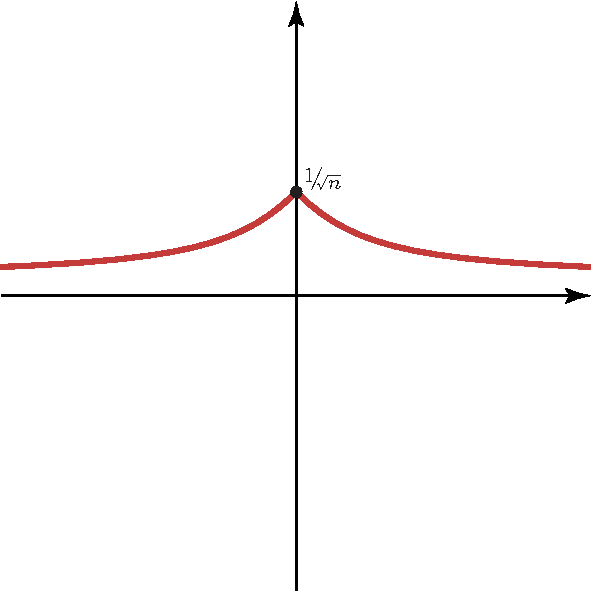
\includegraphics[trim=0cm 4cm 0cm 0cm, clip, scale=0.8]{images/grafico1.pdf}
\end{center}
		Segue chiaramente che
		\begin{equation*}
			\sup_{x\in \realset}\phi_n\left(x\right)=\phi_n\left(0\right)=\frac{1}{\sqrt{n}}\left( =c_n\right)
		\end{equation*}
	\item Calcoliamo il limite per $n\to +\infty$:
	\begin{equation*}
		\lim_{n\to+\infty}\left(\sup_{x\in A}\abs{f_n\left(x\right)-f\left(x\right)}\right)=\lim_{n\to+\infty}\frac{1}{\sqrt{n}}=0
	\end{equation*}
	\end{enumerate}
Abbiamo così verificato la convergenza richiesta.
\end{example}
%fINO A QUI
\begin{example}{\textsc{Successione geometrica.}}~{}\\
	Consideriamo $f_n\left(x\right)=x^n,\ \forall n\geq 0$. Allora:
	\begin{enumerate}
		\item $x^n$ converge uniformemente a $0$ su \textit{ogni} insieme $\left[-a,a\right],\ \forall a\colon 0<a<1$.
		\item $x^n$ \textbf{non} converge uniformemente a $0$ su $\left(-1,1\right)$.
	\end{enumerate}
\end{example}
\begin{demonstration}~{}\\
	\begin{enumerate}
		\item Sia $a\in\left(0,1\right)$ fissato e consideriamo
		\begin{equation*}
			\abs{x^n-0}=\abs{x^n}\implies\sup_{x\in \left[-a,a\right]}\abs{x^n-0}=\sup_{x\in \left[-a,a\right]}\abs{x^n}
		\end{equation*}
		Qual è il grafico di $x^n$?\\
		\begin{minipage}{0.75\textwidth}
			\begin{itemize}
				\item Se $n$ \textbf{pari}, è visivamente simile a quello di $x^2$.
			\end{itemize}
		\end{minipage}\hspace{-7mm}
		\begin{minipage}{0.15\textwidth}
			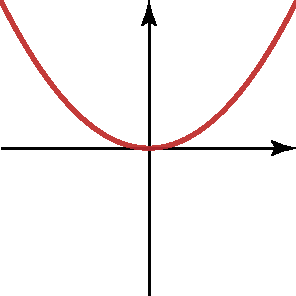
\includegraphics[trim=0cm 0cm 0cm 0cm, clip, scale=0.5]{images/grafico2a.pdf}
		\end{minipage}\\
			\begin{minipage}{0.75\textwidth}
		\begin{itemize}
			\item Se $n$ \textbf{dispari}, è visivamente simile a quello di $x^3$.
		\end{itemize}
	\end{minipage}\hspace{-7mm}
	\begin{minipage}{0.15\textwidth}
		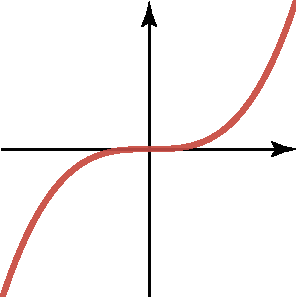
\includegraphics[trim=0cm 0cm 0cm 0cm, clip, scale=0.5]{images/grafico2b.pdf}
	\end{minipage}\\

		Tuttavia per $\abs{x^n},\ \forall n\geq 2$, che è una funzione pari, il grafico è visivamente simile a quello di $x^2$.
		Segue immediatamente che
		\begin{equation*}
			\sup_{x\in \left[-a,a\right]}\abs{x^n}=a^n,\ \forall a\colon 0<a<1
		\end{equation*}
		Ora si ha
		\begin{equation*}
			\lim_{n\to+\infty}\left(\sup_{x\in \left[-a,a\right]}\abs{x^n}\right)=\lim_{n\to+\infty}a^n=0
		\end{equation*}
		perché $a\in\left(0,1\right)$ e quindi $a^n$ è una successione geometrica convergente e pertanto il limite a $+\infty$ è sempre necessariamente 0.
		\item In questo caso
		\begin{equation*}
			\sup_{x\in\left(-1,1\right)}\abs{x^n}=1,\ \forall n
		\end{equation*}
		da cui
		\begin{equation*}
			\lim_{n\to+\infty}\left(\sup_{x\in\left(-1,1\right)}\abs{x^n}\right)=1\neq 0
		\end{equation*}
	pertanto \textit{non} c'è convergenza uniforme su $\left(-1,1\right)$.
	\end{enumerate}
\end{demonstration}
\subsection{Eserciziamoci! Convergenza uniforme}
\begin{exercise}
	$f_n\left(x\right)=\frac{x^n}{n}$ converge uniformemente a $0$ su $\left[0,1\right]$?
\end{exercise}
\begin{solution}
	Dimostriamo che
	\begin{equation*}
		\lim_{n\to+\infty}\left(\sup_{x\in \left[0,1\right]}\abs{\frac{x^n}{n}-0}\right)=\lim_{n\to+\infty}\left(\sup_{x\in \left[0,1\right]}\frac{x^n}{n}\right)=0
	\end{equation*}
	Poiché
	\begin{equation*}
		\sup_{x\in \left[0,1\right]}\frac{x^n}{n}=\frac{x^n}{n}\left.\right|_{x=1}\,=\frac{1}{n}
	\end{equation*}
	allora
	\begin{equation*}
	\lim_{n\to+\infty}\left(\sup_{x\in \left[0,1\right]}\frac{x^n}{n}\right)=\lim_{n\to+\infty}\frac{1}{n}=0
	\end{equation*}
\end{solution}
\subsection{Criterio di Cauchy per la convergenza uniforme}
Come nel caso delle successioni numeriche, esiste un \textbf{criterio di Cauchy} per la convergenza uniforme.
\begin{theorema}[Criterio di Cauchy per la convergenza uniforme.]~{}\\\label{criteriodicauchyperconvergenzauniforme}\index{criterio!di Cauchy!per la convergenza uniforme}
	Siano $\funz{f_n}{A\subseteq\realset}{\realset}$. Allora
	\begin{multline}
		f_n\text{ converge uniformemente su }A \iff\\
		\iff\forall \epsilon >0\ \exists N=N\left(\epsilon\right)\colon\forall n,m\geq N\ \abs{f_n\left(x\right)-f_m\left(x\right)}<\epsilon,\ \forall x\in A
	\end{multline}
\end{theorema}
\begin{observe}
Il criterio di Cauchy è un \textit{risultato teorico molto importante}, in quanto permette di mostrare la convergenza uniforme di una successione di funzioni \textit{senza sapere} quale sia il limite come invece è necessario nella definizione di convergenza, in modo analogo a ciò che succede con il criterio di Cauchy per le \textit{successioni numeriche}.
\end{observe}
\subsection{Visualizzazione della convergenza uniforme}
Siamo abituati alle successioni numeriche $v_n$ ed eventualmente a studiare il loro andamento in modo grafico, rappresentando sulle ascisse il numero $n$ e sulle ordinate il valore $v_n$. Nel caso di successioni di funzioni l'argomento è una funzione, quindi per studiarle può essere utile proprio disegnare i grafici degli $f_n$ e come convergono verso $f$.\\
Come appare \textit{visivamente} la convergenza uniforme? Possiamo riscrivere la condizione della convergenza uniforme
\begin{equation*}
	\forall \epsilon>0\ \exists N=N\left(\epsilon\right)\ \forall n\geq N\ \abs{f_n\left(x\right)-f\left(x\right)}<\epsilon,\ \forall x\in A
\end{equation*}
come
\begin{equation}
	f\left(x\right)-\epsilon<f_n\left(x\right)<f\left(x\right)+\epsilon,\ \forall x\in A\text{ definitivamente}
\end{equation}
In altre parole, $f_n$ deve essere compresa nell'\textbf{intorno tubulare} di $f\left(x\right)$ definitivamente, nel senso che le $f_n$ devono stare in questo intorno per ogni $n$ sufficientemente grande (cioè $\forall n\geq N$).
\begin{center}
	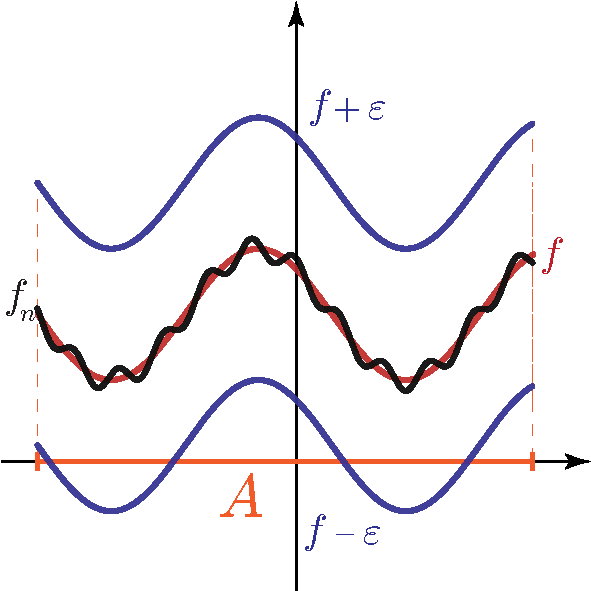
\includegraphics[trim=0cm 0cm 0cm 0cm, clip, scale=0.65]{images/grafico3.pdf}
\end{center}
\begin{define}[Intorno tubulare.]~{}\\
Un \textbf{intorno tubulare}\index{intorno!tubulare} di larghezza $\epsilon$ di una curva è l'unione di tutti i dischi di raggio $\epsilon$ con centro un punto di una curva.
\end{define}
\subsection{Generalizzazioni della convergenza uniforme}\label{sec:generalizzazioni-della-convergenza-uniforme}
Prima di tutto, ricordiamo le definizioni di norma e spazio normato.
\begin{define}[Spazio normato e norma.]~{}\\
	Uno \textbf{spazio normato}\index{spazio!normato} è una coppia $\left(X,\ \norm{\cdot}\right)$ dove $X$ è un spazio vettoriale su $\kamp$ reale o complesso e $\funz{\lvert\lvert\cdot\rvert\rvert}{X}{\realset^+}$ è una funzione detta \textbf{norma}\index{norma}, cioè tale che $\forall x,\ y\in X,\ \lambda\in\kamp$ essa soddisfi le seguenti proprietà:
	\begin{enumerate}
		\item $\norm{x}\geq 0,\ \norm{x}=0\iff x=0$.
		\item $\norm{\lambda x}=\abs{\lambda}\norm{x}$.
		\item $\norm{x+y}\leq\norm{x}+\norm{y}$.
	\end{enumerate}
\end{define}
	\begin{observe}
	Ogni spazio normato è anche uno spazio metrico se consideriamo la \textbf{metrica indotta dalla norma}\index{metrica!indotta dalla norma}, cioè la funzione data da $\mvf{d}{x}{y}\coloneqq\norm{x-y}$.
\end{observe}
Generalizziamo la definizione di convergenza uniforme considerando $\funz{f_n,\ f}{A}{Y}$, con $A$ \textit{insieme qualsiasi} e $Y$ uno spazio \textit{normato}; se vogliamo che valga anche il criterio di Cauchy è necessario che $Y$ sia \textit{anche} uno spazio \textbf{completo}.
\begin{define}[Successione di Cauchy.]~{}\\
		Una successione $v_n\in X$ è \textbf{di Cauchy}\index{successione!di Cauchy} in $X$ se
	\begin{equation}
		\forall \epsilon >0\ \exists N=N\left(\epsilon\right)\colon \forall n,m\geq N\ \mvf{d}{v_n}{v_m}<\epsilon
	\end{equation}
\end{define}
\begin{define}[Spazio completo.]~{}\\
	Uno spazio metrico è detto \textbf{completo}\index{spazio!metrico!completo} se tutte le successioni di Cauchy convergono.
\end{define}
\begin{observe}
	Una successione convergente è \textit{sempre} di Cauchy, ma in generale \textit{non tutte} le successioni di Cauchy convergono. L'implicazione opposta è vera solo se lo spazio è completo.
\end{observe}
Possiamo ora, date queste nuove ipotesi, riformulare la convergenza uniforme.
\begin{define}[Convergenza uniforme, generalizzata.]~{}\\
		Siano $\funz{f_n,\ f}{A}{Y}$ con $A$ insieme qualsiasi e $Y$ spazio normato (completo). Si dice che $f_n$ \textbf{converge uniformemente}\index{convergenza!uniforme} a $f$ \textbf{su} $A$ se
	\begin{equation}
		\forall \epsilon >0\ \exists N=N\left(\epsilon\right)\colon \forall n\geq N\ \norm{f_n\left(x\right)-f\left(x\right)}<\epsilon,\ \forall x\in A
	\end{equation}
\end{define}
\begin{digression}
	Volendo è possibile generalizzare ulteriormente parlando di convergenza uniforme per funzioni a valori in semplici \textbf{spazi metrici} (completi), sostituendo a $\norm{f_n\left(x\right)-f\left(x\right)}<\epsilon$ la condizione $\mvf{d}{f_n\left(x\right)}{f\left(x\right)}<\epsilon$. Nei nostri studi non affronteremo ciò e ci limiteremo a considerare il caso di spazi normati (completi).
\end{digression}
\section{Convergenza puntuale}
Durante gli studi di \textsc{Calcolo delle probabilità} si è parlato di tre tipi di convergenze di successioni di variabili aleatorie: la \textbf{convergenza in probabilità}, la \textbf{convergenza quasi certa} e la \textbf{convergenza in legge} (o in distribuzione). Consideriamo ora quest'ultima, di cui riportiamo la definizione.
\begin{define}[Convergenza in legge.]~{}\\
	Dato $\left(\Omega,\ \mathcal{M},\ \mathbb{P}\right)$ spazio di probabilità, $\funz{X_n,\ X}{\Omega}{\realset}$ variabili aleatorie e le due corrispettive \textit{funzioni di distribuzione}
	\begin{gather*}
		\funztot{F_n}{\realset}{\realset}{x}{F_n\left(x\right)=\mathbb{P}\left(X_n\leq x\right)\ \forall x\in \realset}\\
		\funztot{F}{\realset}{\realset}{x}{F_n\left(x\right)=\mathbb{P}\left(X\leq x\right)\ \forall x\in \realset}\\
	\end{gather*}
allora si dice che $X_n$ converge a $X$ \textbf{in legge}\index{convergenza!in legge} $\left(X_n\stackrel{d}{\to}X\right)$ se
\begin{equation}
	\lim_{n\to+\infty}F_n\left(x\right)=F\left(x\right),\ \forall x\in\realset\ \text{punto di continuità di }F.
\end{equation}
\end{define}
Quello che abbiamo appena scritta non è altro che il caso applicato agli \textit{studi probabilistici} della \textbf{convergenza puntuale} di una successione ad una funzione limite nel punto $x$.
\begin{define}[Convergenza puntuale.]~{}\\
	Siano $\funz{f_n,\ f}{A}{Y}$ con $A$ insieme qualsiasi e $Y$ spazio normato (completo). $f_n$ converge a $f$ \textbf{puntualmente}\index{convergenza!puntuale} in ogni punto di $A$ se
	\begin{equation}
		\forall x\in A\ \forall \epsilon>0\ \exists N=N\left(\epsilon,x\right)\colon\forall n\geq N\ \norm{f_n\left(x\right)-f\left(x\right)}<\epsilon
	\end{equation}
\end{define}
Confrontiamo qui $\funz{f_n,\ f}{A\subseteq R}{\realset}$:
\begin{enumerate}
	\item \textbf{(CU)} $f_n$ converge a $f$ \textbf{uniformemente} su $A$ se
	\begin{equation*}
		\forall \epsilon>0\ \exists N=N\left(\epsilon\right)\colon\forall n\geq N\ \abs{f_n\left(x\right)-f\left(x\right)}<\epsilon,\ \forall x\in A
	\end{equation*}
	\item \textbf{(CP)} $f_n$ converge a $f$ \textbf{puntualmente} in ogni punto di $A$ se
	\begin{equation*}
		\forall x\in A\ \forall \epsilon>0\ \exists N=N\left(\epsilon,x\right)\colon\forall n\geq N\ \abs{f_n\left(x\right)-f\left(x\right)}<\epsilon
	\end{equation*}
\end{enumerate}
Il quantificatore esistenziale $\exists$ implica che ciò che esiste dipende da tutto ciò che lo precede: nella convergenza puntuale $N$ non dipende dal solo $\epsilon$ come così capita nella \textbf{convergenza uniforme}, ma anche da $x$. La convergenza uniforme è più restrittiva rispetto alla puntuale.
\begin{observe}
	Questa differenza è concettualmente analoga a quella che c'è fra continuità uniforme e continuità.
\end{observe}
\begin{observe}
	Possiamo considerare $\forall \epsilon >0$ due punti $x'$ e $x''$ su cui valutare la \textbf{soglia} $N$ di un successione di funzioni: in questo caso abbiamo per il primo punto $N\left(\epsilon,\ x'\right)$ e per il secondo $N\left(\epsilon,\ x''\right)$. Vediamo subito che $\max\left(N\left(\epsilon,\ x'\right),N\left(\epsilon,\ x''\right)\right)$ è una soglia lecita sia per $x'$ sia $x''$.\\
	In generale, se voglio passare dalla convergenza puntuale alla convergenza uniforme devo considerare
	\begin{equation*}
		\sup_{x\in A}N\left(\epsilon, x\right)
	\end{equation*}
\begin{itemize}
	\item Se $A$ è finito, allora $\displaystyle\sup_{x\in A}N\left(\epsilon\right)=\max_{x\in A}N\left(\epsilon\right)=N\left(\epsilon\right)$ e c'è convergenza uniforme.
	\item Se $\displaystyle\sup_{x\in A}N\left(\epsilon\right)=+\infty$ allora \textit{non} c'è convergenza uniforme.
\end{itemize}
\end{observe}
Dalle definizioni segue immediatamente che
	\begin{multline}
	f_n\text{ converge uniformemente a }f\text{ in }A\implies\\
	\implies f_n\text{ converge puntualmente a }f\text{ in ogni punto di }A
\end{multline}
ma in generale vale che la convergenza puntuale \textbf{NON} implica la convergenza uniforme.
\begin{example}[Successione geometrica e convergenza puntuale.]~{}
	Consideriamo la successione geometrica $f_n\left(x\right)=x^n,\ \forall n\geq 0$.\\
	$\forall x\in\realset$ fissato si ha
	\begin{equation*}
		\lim_{n\to+\infty}x^n=
		\begin{cases}
			\begin{array}{ll}
				+\infty&\text{se }x>1\\
				1&\text{se }x=1\\
				0&\text{se }-1<x<1\\
				\text{non esiste}&\text{se }x\leq 1
			\end{array}
		\end{cases}
	\end{equation*}
Allora $x^n$ converge puntualmente a
\begin{equation*}
	f\left(x\right)=
	\begin{cases}
	1&\text{se }x=1\\
	0&\text{se }-1<x<1	
	\end{cases}
\end{equation*}
in ogni punto di $\left(-1,1\right]$.
\begin{center}
	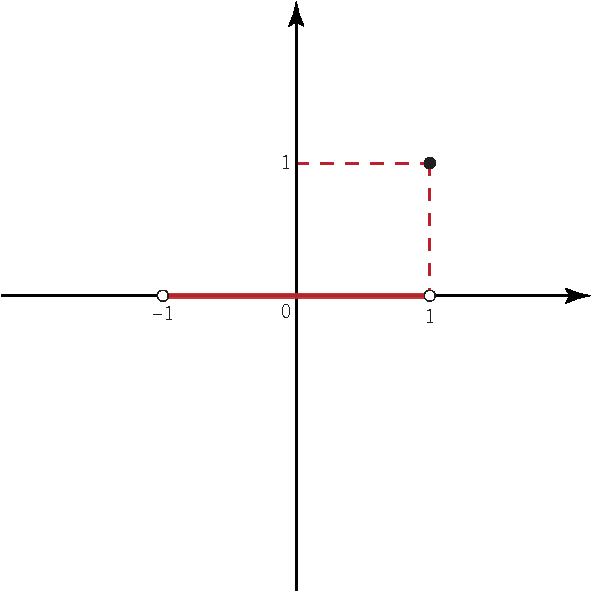
\includegraphics[trim=0cm 4cm 0cm 0cm, clip, scale=0.65]{images/grafico4.pdf}
\end{center}
\end{example}
Abbiamo provato precedentemente che $f_n\left(x\right)=x^n$ converge uniformemente a $f\equiv 0$ in ogni intervallo $\left[-a,a\right]\subsetneqq\left(-1,1\right),\ \forall a\in\left(0,1\right)$, ma \textit{non} converge uniformemente a $f=0$ in $\left(-1,1\right)$.\\
Questo mostra che su $\left(-1,1\right)$ c'è convergenza puntuale ma non uniforme.
\begin{observe}
	Questo esempio mostra inoltre che la CP \textit{non} è sufficiente in generale per trasferire la continuità alla funzione limite.
\end{observe}
\section{Proprietà di regolarità nel caso di convergenza uniforme e puntuale}
Adesso studiamo il diverso comportamento delle due tipologie di convergenza viste rispetto alle proprietà enunciate nel titolo di questa sezione: se le funzioni $f_n$ della successione sono limitate/continue/integrabili/differenziabile, la funzione limite $f$ è limitata/continua/integrabile/differenziabile?
\subsection{Limitatezza}
\begin{theorema}[Teorema di limitatezza per successioni.]~{}\\
Siano $\funz{f_n,f}{\left[a,b\right]}{\realset},\ n\geq 1$ tali che
\begin{enumerate}
	\item $f_n$ limitata su $\left[a,b\right],\ \forall n\geq 1$.
	\item $f_n$ converge uniformemente a $f$ su $\left[a,b\right]$.
\end{enumerate}
Allora $f$ è limitata su $\left[a,b\right]$.
\end{theorema}
\begin{demonstration}
	Dobbiamo provare che
	\begin{equation*}
		\exists n>0\colon \abs{f(x)}\leq n,\ \forall x\in A
	\end{equation*}
Per l'ipotesi $2)$ sappiamo che
\begin{equation*}
	\forall \epsilon>0\ \exists N=N\left(\epsilon\right)\colon\forall n\geq N\ \abs{f_n\left(x\right)-f\left(x\right)}<\epsilon,\ \forall x\in A
\end{equation*}
Posto ad esempio\footnote{La scelta di $\epsilon$ è assolutamente arbitraria.} $\epsilon = 2$, consideriamo la soglia $N_2=N\left(2\right)$ e $n=N_2$. Allora la relazione precedente risulta
\begin{equation*}
	\abs{f_{N_2}\left(x\right)-f\left(x\right)}<2,\ \forall x\in A
\end{equation*}
Consideriamo $f_{N_2}\left(x\right)$: per l'ipotesi $1)$ è limitata, cioè
\begin{equation*}
	\exists n_2>0\colon \abs{f_{N_2}(x)}\leq n,\ \forall x\in A
\end{equation*}
Per ogni $x\in A$ si ha quindi
\begin{equation*}
	\abs{f\left(x\right)}=\abs{f\left(x\right)+f_{N_2}(x)-f_{N_2}(x)}\leq\abs{f\left(x\right)-f_{N_2}(x)}+\abs{f_{N_2}(x)}\leq 2+n_2=n,\ \forall x\in A
\end{equation*}
\end{demonstration}
\begin{digression}
	Il risultato si generalizza ponendo $\funz{f_n,f}{X}{Y}$, dove $X$ è un qualunque insieme e $Y$ è uno spazio normato.
\end{digression}
La convergenza puntuale non è sufficiente per trasferire la limitatezza alla funzione limite: infatti, possiamo costruire un controesempio di una successione $f_n$ limitata che converge puntualmente ad una funzione non limitata.
\begin{example}
	Sia $\funz{f_n}{\left(0,1\right]}{\realset},\ n\geq1$, definita da
	\begin{equation*}
		f_n\left(x\right)=\begin{cases}
			\begin{array}{ll}
				n&\text{se }0<x<\frac{1}{n}\\
				\frac{1}{x}&\text{se }x\geq\frac{1}{n}\\
			\end{array}
		\end{cases}
	\end{equation*}
$\forall x\in \left(0,1\right]$.\\
Un grafico qualitativo di $f_n$ è rappresentato in figura.
\begin{center}
	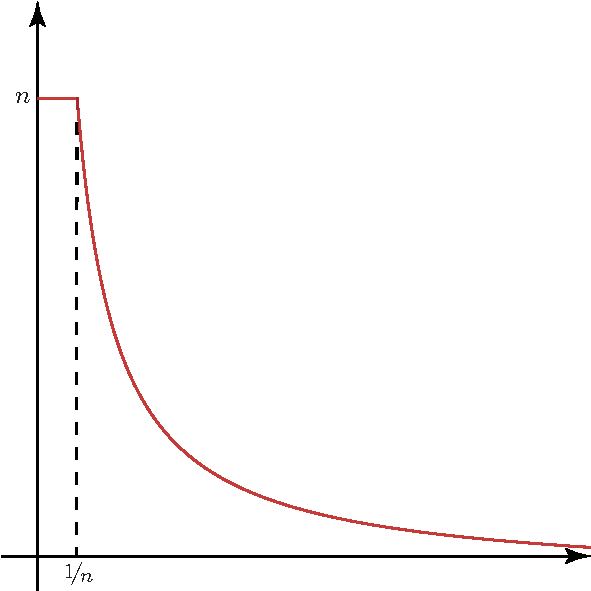
\includegraphics[trim=0cm 0cm 0cm 0cm, clip, scale=0.65]{images/grafico5.pdf}
\end{center}
Per ogni $n\geq1$ la funzione $f_n$ è limitata su $\left(0,1\right]$. Inoltre, $\forall x\in \left(0,1\right]$ si ha
	
	\begin{equation*}
		\lim_{n\to+\infty}f_n\left(x\right)=\frac{1}{x}
	\end{equation*}
	Infatti, fissato $x\in \left(0,1\right]$, indicando con le parentesi quadre la \textit{parte intera} e posto 
	\begin{equation*}
	n_x=\left[\frac{1}{x}\right]+1
	\end{equation*}
	allora se $n\geq n_x$ si ha $x>1/n$ e dunque
	\begin{equation*}
	f_n\left(x\right)=\frac{1}{x}
	\end{equation*}
	Si ha dunque
	\begin{equation*}
		\lim_{n\to+\infty}f_n\left(x\right)=\lim_{n\to+\infty}\frac{1}{x}=\frac{1}{x}
	\end{equation*}
	La successione di funzioni \textit{limitate} $f_n$ converge quindi puntualmente $\forall x\in \left(0,1\right]$ alla funzione $\frac{1}{x}$ che \textbf{non} è limitata su $\left(0,1\right]$.
\end{example}
\subsection{Continuità}
\begin{theorema}[Teorema di continuità per successioni.]~{}\\
	Siano $\funz{f_n,f}{\left[a,b\right]}{\realset},\ n\geq 1$ tali che
	\begin{enumerate}
		\item $f_n$ continua su $\left[a,b\right],\ \forall n\geq 1$.
		\item $f_n$ converge uniformemente a $f$ su $\left[a,b\right]$.
	\end{enumerate}
	Allora $f$ è continua su $\left[a,b\right]$.
\end{theorema}
\begin{demonstration}
	Sia $x_0\in\left[a,b\right]$ fissato. Dobbiamo dimostrare che
	\begin{equation*}
		\forall \epsilon>0\ \exists \delta>0 \colon \abs{x-x_0}<\delta\implies \abs{f\left(\right)-f\left(x_0\right)}<\epsilon
	\end{equation*}
	Per l'ipotesi $2)$ sappiamo che $f_n$ converge uniformemente; allora, fissato $\epsilon>0$, $\exists N=N\left(\epsilon\right)\in\naturalset$ tale che
	\begin{equation*}
		\abs{f_N\left(x\right)-f\left(x\right)}<\frac{\epsilon}{3},\ \forall x\in\left[a,b\right]
	\end{equation*}
Questa relazione chiaramente vale anche per $x_0$:
	\begin{equation*}
	\abs{f_N\left(x_0\right)-f\left(x_0\right)}<\frac{\epsilon}{3}
\end{equation*}
Per l'ipotesi $1)$ ogni $f_n$ è continua in $x_0$, in particolare $f_N$ la è. Per definizione di continuità, considerato sempre lo stesso $\epsilon>0$ di prima $\exists\delta >0$ tale che se $\abs{x-x_0}<\delta$ si ha
	\begin{equation*}
	\abs{f_N\left(x\right)-f_N\left(x_0\right)}<\frac{\epsilon}{3}
\end{equation*}
Quindi, se $\abs{x-x_0}<\delta$ abbiamo
\begin{equation*}
	\abs{f\left(x\right)-f\left(x_0\right)}\leq\abs{f\left(x\right)-f_N\left(x\right)}+\abs{f_N\left(x\right)-f_N\left(x_0\right)}+\abs{f_N\left(x_0\right)-f\left(x_0\right)}\leq\frac{\epsilon}{3}+\frac{\epsilon}{3}+\frac{\epsilon}{3}=\epsilon
\end{equation*}
\end{demonstration}
\begin{digression}
	Il risultato si generalizza ponendo $\funz{f_n,f}{X}{Y}$, dove $X$ è un qualunque insieme e $Y$ è uno spazio normato.
\end{digression}
La convergenza puntuale non è sufficiente per trasferire la continuità alla funzione limite: infatti, possiamo costruire un controesempio di una successione $f_n$ continua che converge puntualmente ad una funzione non continua.
\begin{example}
Consideriamo la successione geometrica $f_n(x)=x^n,\ n\geq1$, sull'intervallo $[0,1]$.\\
Sappiamo che essa converge puntualmente in ogni punto di $[0,1]$ alla funzione limite 
\begin{equation*}
	f\left(x\right)=
	\begin{cases}
		\begin{array}{ll}
			0&\text{se }0\geq x < 1\\
			1<&\text{se }x=1
		\end{array}
	\end{cases}
\end{equation*}
La successione di funzioni \textit{continue} $f_n$ converge quindi puntualmente per ogni $x\in[0,1]$ alla funzione $f$ che \textbf{non} è continua su $[0,1]$.
\end{example}
\subsection{Integrabilità e passaggio al limite sotto segno di integrale}
\begin{theorema}[Teorema di integrabilità per successioni, passaggio al limite sotto segno di integrale.]~{}\\
	Siano $\funz{f_n,f}{\left[a,b\right]}{\realset},\ n\geq 1$ tali che
	\begin{enumerate}
		\item $f_n\in\mathcal{R}\left(\left[a,b\right]\right),\ \forall n\geq 1$.
		\item $f_n$ converge uniformemente a $f$ su $\left[a,b\right]$.
	\end{enumerate}
	Allora
	\begin{enumerate}
		\item $f\in\mathcal{R}\left(\left[a,b\right]\right)$.
		\item Vale il \textbf{passaggio al limite sotto segno di integrale}\index{passaggio al limite sotto segno di integrale}:
		\begin{equation}
			\lim_{n\to+\infty}\int_{a}^{b}f_n\left(x\right)=\int_{a}^{b}lim_{n\to+\infty}f_n\left(x\right)dx=\int_{a}^{b}f\left(x\right)dx
		\end{equation}
	\end{enumerate}
\end{theorema}
Vedremo la dimostrazione di una versione più generica del teorema quando parleremo degli integrali di Lebesgue.\\
Per quanto questo teorema ha una notevole importanza, ha un campo d'azione particolarmente limitato. Infatti, anche cambiando leggermente le ipotesi non è più possibile affermare la tesi. Vediamo alcuni di questi controesempi.
\begin{example}
	La convergenza uniforme \textit{non} è sufficiente per trasferire alla funzione limite l'integrabilità su un intervallo \textit{illimitato}.\\
	Consideriamo la successione di funzioni $\funz{f_n}{\left[1,+\infty\right)}{\realset}$ definite da
\begin{equation*}
	f_n(x)=\frac{n}{nx+x^2},\ \forall x\geq1, n\geq1 
\end{equation*}
Per ogni $x\geq 1$ osserviamo che $f_n(x)\sim \frac{n}{nx}$ per $n\to+\infty$, quindi si ha
\begin{equation*}
	\lim_{n\to+\infty}f_n\left(x\right)=\lim_{n\to+\infty}\frac{n}{nx}=\frac{1}{x}
\end{equation*}
Si ha quindi convergenza puntuale in ogni punto di $\left[1,+\infty\right)$ alla funzione $f(x)=\frac{1}{x}$. Inoltre, la convergenza è uniforme su $\left[1,+\infty\right)$: vale infatti
\begin{equation*}
	\abs{f_n(x)-f(x)}=\abs{\frac{n}{nx+x^2}-\frac{1}{x}}=\frac{1}{n+x}
\end{equation*}
per ogni $x\geq1$, $n\geq1$. Per \textit{monotonia}, si ha quindi
\begin{equation*}
	\sup_{x\geq 1}\abs{f_n(x)-f(x)}=\sup_{x\geq1}\frac{1}{n+x}=\frac{1}{n+1},\ \forall n\geq1
\end{equation*}
Deduciamo che
\begin{equation*}
	\lim_{n\to+\infty}\left(\sup_{x\geq1}\abs{f_n(x)-f(x)}\right)=\lim_{n\to+\infty}\frac{1}{n+1}=0
\end{equation*}		
	da cui segue la convergenza uniforme su $\left[1,+\infty\right)$.
	Osserviamo ora che per ogni $n\geq1$ si ha
	\begin{equation*}
		f_n(x)\sim \frac{n}{x^2},\ x\to+\infty
	\end{equation*}
	e dunque $f_n$ è integrabile in senso improprio su $[1,+\infty)$, per ogni $n\geq1$; la funzione limite $f(x)=\frac{1}{x}$ \textit{non} è invece integrabile in senso improprio su $[1,+\infty)$.\\
	La successione di funzioni $f_n$ \textit{integrabili} su $[1,+\infty)$ converge quindi uniformemente su $[1,+\infty)$ alla funzione $f$ che \textbf{non} è integrabile su $[1,+\infty)$.
\end{example}
\begin{example}
	La convergenza uniforme \textit{non} è condizione necessaria per il passaggio al limite sotto segno di integrale.\\
	Consideriamo la successione di funzioni $f_n\left(x\right)=x^n$ definite su $\left[0,1\right]$. Osserviamo che
	\begin{equation*}
		\lim_{n\to+\infty}\int_{0}^{1}x^ndx=\lim_{n\to+\infty}\left[\frac{1}{n+1}x^{n+1}\right]_{0}^{1}=\lim_{n\to+\infty}\frac{1}{n+1}=0
	\end{equation*}
Invece, sappiamo che $x^n$ converge puntualmente in ogni punto di $[0,1]$ alla funzione limite 
\begin{equation*}
	f\left(x\right)=
	\begin{cases}
		\begin{array}{ll}
			0&\text{se }0\geq x < 1\\
			1<&\text{se }x=1
		\end{array}
	\end{cases}
\end{equation*}
dunque su $[0,1]$ $f\left(x\right)=\lim_{n\to\infty}f_n\left(x\right)$ è una funzione \textit{identicamente nulla} tranne un \textit{numero finito} di punti (in questo caso, uno soltanto). Allora
\begin{equation*}
	\int_{0}^{1}\lim_{n\to+\infty}x^ndx=\int_{0}^{1}0dx=0
\end{equation*}
 $x^n$ non converge uniformemente su $[\left[0,1\right]$, ma il passaggio al limite sotto segno di integrale si verifica comunque.
\end{example}
\begin{example}
	Consideriamo la successione di funzioni $f_n\left(x\right)=x^n$ definite su $\left[0,1\right]$. Osserviamo che
	\begin{equation*}
		\lim_{n\to+\infty}\int_{0}^{1}x^ndx=\lim_{n\to+\infty}\left[\frac{1}{n+1}x^{n+1}\right]_{0}^{1}=\lim_{n\to+\infty}\frac{1}{n+1}=0
	\end{equation*}
	Invece, sappiamo che $x^n$ converge puntualmente in ogni punto di $[0,1]$ alla funzione limite 
	\begin{equation*}
		f\left(x\right)=
		\begin{cases}
			\begin{array}{ll}
				0&\text{se }0\geq x < 1\\
				1<&\text{se }x=1
			\end{array}
		\end{cases}
	\end{equation*}
	dunque su $[0,1]$ $f\left(x\right)=\lim_{n\to\infty}f_n\left(x\right)$ è una funzione \textit{identicamente nulla} tranne un \textit{numero finito} di punti (in questo caso, uno soltanto). Allora
	\begin{equation*}
		\int_{0}^{1}\lim_{n\to+\infty}x^ndx=\int_{0}^{1}0dx=0
	\end{equation*}
	$x^n$ non converge uniformemente su $[\left[0,1\right]$, ma il passaggio al limite sotto segno di integrale si verifica comunque.
\end{example}
\begin{example}
	La convergenza uniforme \textit{non} è condizione sufficiente per il passaggio al limite sotto il segno di integrale nel caso in un intervallo \textit{illimitato}.
	Sia $\funz{f_n}{\left[0,+\infty\right)}{\realset}$, $n\geq1$, definita da
	\begin{equation*}
		f_n\left(x\right)=\begin{cases}
			\begin{array}{ll}
				\frac{1}{n}&\text{se }n\geq x\geq2n\\
				\frac{1}{x}&\text{se }x<n\vee x>2n
			\end{array}
		\end{cases}
	\end{equation*}
Osserviamo che
\begin{align*}
	\lim_{n\to+\infty}\int_{0}^{+\infty}f_n\left(x\right)dx=&\lim_{n\to+\infty}\left[\int_{0}^{n}0dx+\int_{n}^{2n}\frac{1}{n}dx+\int_{2n}^{+\infty}0dx\right]=\lim_{n\to+\infty}\int_{n}^{2n}\frac{1}{n}dx=\\
	=&\lim_{n\to+\infty}\left[\frac{x}{n}\right]_{n}^{2n}=\lim_{n\to+\infty}\frac{2n--n}{n}=\lim_{n\to+\infty}1=1
\end{align*}
Invece, si vede immediatamente che
	\begin{equation*}
	\int_{0}^{+\infty}\lim_{n\to+\infty}f_n\left(x\right)dx=\int_{0}^{+\infty}0dx=0
\end{equation*}
Vediamo che $f_n$ converge uniformemente su $\left[0,+\infty\right)$ a $0$:
\begin{gather*}
	\sup_{x\in\left[0,+\infty\right)}\abs{f_n\left(x\right)-f\left(x\right)}=\frac{1}{n}\\
	\lim_{n\to+\infty}\left(\sup_{x\in\left[0,+\infty\right)}\right)=\lim_{n\to+\infty}\frac{1}{n}=0
\end{gather*}
Anche aggiungendo al teorema l'ipotesi che $f\left(x\right)$ sia Riemann-integrabile (in questo caso ciò è verificato), il passaggio al limite sotto segno di integrale \textit{non} si verifica \textit{necessariamente} se l'intervallo è illimitato.
\end{example}
\begin{example}
	La convergenza puntuale \textit{non} è condizione sufficiente per il passaggio al limite sotto il segno di integrale, nemmeno nel caso di un intervallo limitato.
	Consideriamo la successione di funzioni $f_n\left(x\right)=nx\left(1-x^2\right)^n$ definite su $\left[0,1\right]$. Osserviamo che
	\begin{align*}
		\lim_{n\to+\infty}\int_{0}^{1}nx\left(1-x^2\right)^ndx=&-\frac{1}{2}\lim_{n\to+\infty}\int_{0}^{1}n\left(-2x\right)\left(1-x^2\right)^n=\\
		=&-\frac{1}{2}\lim_{n\to+\infty}n\left[\frac{1}{n+1}\left(1-x^2\right)^{n+1}\right]_{0}^{1}=\frac{1}{2}\lim_{n\to+\infty}\frac{n}{n+1}=\frac{1}{2}
	\end{align*}
Invece, osserviamo che, fissato $x$ rispetto alla $n$ $nx\left(1-x^2\right)^n=x\frac{\left(1-x^2\right)^n}{\frac{1}{n}}$ si può vedere come il rapporto di un esponenziale di ragione (in modulo) minore di 1 con il reciproco di un termine lineare, dunque per $n\to+\infty$ l'esponenziale tende a $0$ molto più velocemente di $\frac{1}{n}$: segue che
	\begin{equation*}
	\int_{0}^{1}\lim_{n\to+\infty}nx\left(1-x^2\right)^ndx=\int_{0}^{1}0dx=0
\end{equation*}
Per lo stesso ragionamento si vede che $f_n\left(x\right)$ converge puntualmente a $0$ per ogni punto di $\left[0,1\right]$, ma \textit{non} si verifica il passaggio al limite sotto segno di integrale.
\end{example}
\subsection{Derivabilità}
Date $\funz{f_n,f}{A\subseteq\realset}{\realset}$ con $f$ la funzione limite di $f_n$ su $A$, possiamo porci due domande:
\begin{enumerate}
	\item $f_n$ derivabile su $A\implies f$ derivabile su $A$?
	\item Vale lo scambio tra derivata e limite?
	\begin{equation*}
		\lim_{n\to+\infty}f'_n\left(x\right)=D\left(\lim_{n\to+\infty}f\left(x\right)\right)
	\end{equation*}
	O, in altre parole, il diagramma seguente è commutativo?
	% https://q.uiver.app/?q=WzAsNCxbMCwwLCJmX24iXSxbMSwwLCJmJ19uIl0sWzAsMSwiXFxsaW1fe25cXHRvK1xcaW5mdHl9Zl9uIl0sWzEsMSwiXFxsaW1fe25cXHRvK1xcaW5mdHl9ZidfbiJdLFswLDEsIkQiXSxbMCwyLCJcXGxpbSIsMl0sWzEsM10sWzIsM11d
\[\begin{tikzcd}
	{f_n} & {f'_n} \\
	{\textcolor{blueill}{\displaystyle\lim_{n\to+\infty}f_n}} & {\displaystyle\lim_{n\to+\infty}f'_n}
	\arrow["D", from=1-1, to=1-2]
	\arrow["\lim"', color={rgb,255:red,46;green,49;blue,146}, from=1-1, to=2-1]
	\arrow["\lim", from=1-2, to=2-2]
	\arrow["D"', color={rgb,255:red,46;green,49;blue,146}, from=2-1, to=2-2]
\end{tikzcd}\]
\end{enumerate}
La risposta ad entrambe domande, a differenza di quanto ci si potrebbe aspettare dati i risultati su limitatezza/continuità/integrabilità, è \textbf{NO}, anche nel caso di \textit{convergenza uniforme}.
\begin{example}
	La convergenza uniforme \textit{non} è condizione sufficiente per trasferire alla funzione limite la derivabilità.\\
	Consideriamo la successione $f_n(x)=\sqrt{x^2+\frac{1}{n}},\ \forall x\in \realset,\ \forall n\geq1$.
	\begin{itemize}
		\item $f_n$ è derivabile.
		\item $f_n$ abbiamo visto\footnote{Si veda pag. \pageref{valoreassolutoesempioconvergenzaassoluta}, sezione \ref{valoreassolutoesempioconvergenzaassoluta}.} converge uniformemente su $\realset$ a $f\left(x\right)=\abs{x}$ che \textit{non} è derivabile in $x=0$.
	\end{itemize}
\end{example}
\begin{example}
	La convergenza uniforme \textit{non} è condizione sufficiente per poter scambiare limite e derivata, anche se si aggiunge l'ipotesi che la funzione limite sia derivabile.\\
	Consideriamo la successione $f_n(x)=\frac{sin\left(nx\right)}{\sqrt{n}},\ \forall x\in \realset,\ \forall n\geq1$.
	\begin{itemize}
		\item $f_n$ è derivabile su $\realset$, $\forall n\geq 1$, e vale
		\begin{equation*}
			f'\left(x\right)=\sqrt{n}\cos\left(nx\right),\ \forall x\in \realset,\ \forall n\geq1
		\end{equation*}
		\item
		\begin{itemize}
			\item $f_n$ converge \textbf{puntualmente} a $f\left(x\right)=0,\ \forall x\in\realset$:
			\begin{equation*}
				\lim_{n\to+\infty}f_n\left(x\right)=\lim_{n\to+\infty}\underbrace{\frac{1}{\sqrt{n}}}_{\to 0}\underbrace{\sin\left(nx\right)}_{\text{limitato}}=0,\ \forall x\in\realset
			\end{equation*}
			\item $f_n$ converge \textbf{uniformemente} a $f\left(x\right)=0,\ \forall x\in\realset$:
			\begin{equation*}
				\lim_{n\to+\infty}\left(\sup_{x\in\realset}\abs{f_n\left(x\right)-f\left(x\right)}\right)=\lim_{n\to+\infty}\left(\sup_{x\in\realset}\abs{\frac{\sin\left(nx\right)}{\sqrt{n}}}\right)=\lim_{n\to+\infty}\frac{1}{\sqrt{n}}=0
			\end{equation*}
		\end{itemize}
		Osserviamo che in entrambi i casi $f\left(x\right)=0$ su $\realset$: questa funzione è chiaramente derivabile e vale
		\begin{equation*}
			D\left(\lim_{n\to+\infty}f_n\left(x\right)\right)=D\left(0\right)=0,\ \forall x\in\realset
		\end{equation*}
	D'altro canto, si ha
	\begin{equation*}
			\lim_{n\to+\infty}D\left(f_n\left(x\right)\right)=\lim_{n\to+\infty}f'_n\left(x\right)=\lim_{n\to+\infty}\sqrt{n}\cos\left(nx\right)
	\end{equation*}
		Ad esempio, per $x=0$ troveremmo
		\begin{equation*}
				\lim_{n\to+\infty}D\left(f_n\left(x\right)\right)=\lim_{n\to+\infty}\sqrt{n}=+\infty
		\end{equation*}
	Quindi non si può per $x=0$ scambiare limite e derivata-
	\end{itemize}
\end{example}
Esiste comunque un legame tra \textit{successioni di funzioni}, \textit{derivabilità} e convergenza uniforme; scopriamo che non è più la successione $f_n$ a convergere uniformemente, bensì sono le derivate $f'$ della successioni a doverlo fare.
\begin{theorema}[Teorema di derivabilità per successioni.]~{}\\
	Siano dati $\funz{f_n}{\left(a,b\right)}{\realset}$ tali che
	\begin{enumerate}
		\item $f_n$ derivabili su $\left(a,b\right)$.
		\item $\exists c\in\left(a,b\right)\colon f_n\left(c\right)$ converge puntualmente.
		\item $f'_n$ converge uniformemente a $g$ su $\left(a,b\right)$.
	\end{enumerate}
Allora
\begin{enumerate}
	\item $\exists\funz{f}{\left(a,b\right)}{\realset}$ tale che $f_n$ converge uniformemente a $f$ su $\left(a,b\right)$.
	\item $f$ è derivabile.
	\item $f'\left(x\right)=g\left(x\right),\ \forall x\in \left(a,b\right)$, ossia
	\begin{equation}
		f'\left(x\right)=\lim_{n\to+\infty}f'_n\left(x\right),\ \forall x\in\left(a,b\right)
	\end{equation}
\end{enumerate}
\end{theorema}
Per dimostrare il teorema, faremo uso di tre strumenti: il \textit{criterio di Cauchy per la convergenza uniforme} (teorema \ref{criteriodicauchyperconvergenzauniforme}, pag. \pageref{criteriodicauchyperconvergenzauniforme}), il \textit{teorema di scambio di limiti} e una conseguenza \textit{teorema di Lagrange}. Enunciamo questi ultimi due.
\begin{theorema}[Teorema di scambio di limiti.]~{}\\
	Dati $\funz{g_n,g}{I\subseteq \realset}{\realset}$ e $c$ punto di accumulazione di $I$, se
	\begin{enumerate}
		\item $g_n$ converge \textit{uniformemente} a $g$ su $I$
		\item Per ogni $n \geq 1$ esiste $L_n\in\realset$ tale che
		\begin{equation*}
			\lim_{x\to c}g_n\left(x\right)=L_n
		\end{equation*}
	\end{enumerate}
	Allora:
	\begin{enumerate}
		\item Esistono finiti
		\begin{equation}
				\lim_{x\to c}g\left(x\right),\qquad\lim_{n\to+\infty}L_n
		\end{equation}
		\item Vale la relazione
		\begin{equation}
			\lim_{x\to c}g\left(x\right)=\lim_{n\to+\infty}L_n
		\end{equation}
		ossia
	\begin{equation}
		\lim_{x\to c}\lim_{n\to+\infty}g_n\left(x\right)=\lim_{n\to+\infty}\lim_{x\to c}g_n\left(x\right)
	\end{equation}
	\end{enumerate}
	
\end{theorema}
\begin{corollary}[Conseguenza al teorema di Lagrange.]~{}\\
Sia $\funz{h}{\left(\alpha,\beta\right)\subseteq\realset}{\realset}$ derivabile in $\left(\alpha,\beta\right)$. Allora:
\begin{equation}
	\forall u,v\in\left(\alpha,\beta\right)\colon\abs{h\left(u\right)-h\left(v\right)}\leq\left(\sup_{x\in\left(\alpha,\beta\right)}\abs{h'\left(x\right)}\right)\abs{u-v}
\end{equation}
\end{corollary}
\begin{demonstration} \textsc{(del Teorema di derivabilità per successioni.)}
\begin{enumerate}
	\item Dimostriamo la \textit{convergenza uniforme} di $f_n$ su $\left(a, b\right)$. Per il Criterio di Cauchy per la convergenza uniforme è sufficiente
	dimostrare che
	\begin{equation*}
		\forall \epsilon >0\ \exists N=N\left(\epsilon\right)\colon\forall n,m\geq N\ \sup_{x\in \left(a,b\right)}\abs{f_n\left(x\right)-f_m\left(x\right)}<\epsilon
	\end{equation*}
Sia $\epsilon>0$. Per ogni $x\in\left(a,b\right)$, preso $c$ come da ipotesi $2)$:
\begin{equation*}
	\abs{f_n\left(x\right)-f_m\left(x\right)}\leq \abs{f_n\left(x\right)-f_m\left(x\right)-\left(f_n\left(c\right)-f_m\left(c\right)\right)}+\abs{f_n\left(c\right)-f_m\left(c\right)}
\end{equation*}
Studiamo il \textit{primo addendo}. Per il \textit{corollario al teorema di Lagrange} si ha
\begin{equation*}
	\abs{f_n\left(x\right)-f_m\left(x\right)-\left(f_n\left(c\right)-f_m\left(c\right)\right)}\leq\left(\sup_{t\in\left(a,b\right)}\abs{x-c}\right)
\end{equation*}
Inoltre, poiché per ipotesi $3)$ $f'_n$ converge uniformemente su $\left(a,b\right)$, si ha per il criterio di Cauchy che
\begin{equation*}
	\forall \epsilon >0\ \exists N_1=N_1\left(\epsilon\right)\colon\forall n,m\geq N_1\ \sup_{x\in \left(a,b\right)}\abs{f'_n\left(x\right)-f'_m\left(x\right)}<\frac{\epsilon}{2\left(b-a\right)}
\end{equation*}
Segue dunque che
\begin{align*}
	\abs{f_n\left(x\right)-f_m\left(x\right)-\left(f_n\left(c\right)-f_m\left(c\right)\right)}&\leq\left(\sup_{t\in\left(a,b\right)}\abs{x-c}\right)\leq\\
	&\leq\frac{\epsilon}{2\left(b-a\right)}\abs{x-c}\leq\frac{\epsilon}{2},\ \forall x\in\left(a,b\right),\ \forall n,m\geq N_1
\end{align*}
Per il \textit{secondo addendo}, dato che per ipotesi $2)$ $f_n$ converge puntualmente in $c$, possiamo applicare il criterio di Cauchy per le successioni:
\begin{equation*}
		\forall \epsilon >0\ \exists N_2=N_2\left(\epsilon\right)\colon\forall n,m\geq N_2\ \abs{f_n\left(c\right)-f'_m\left(c\right)}<\frac{\epsilon}{2}
\end{equation*}
Posto $N=\max\left\{N_1,N_2\right\}$, per ogni $n,m\geq N$ si ha
\begin{align*}
	\abs{f_n\left(x\right)-f_m\left(x\right)}&\leq \abs{f_n\left(x\right)-f_m\left(x\right)-\left(f_n\left(c\right)-f_m\left(c\right)\right)}+\abs{f_n\left(c\right)-f_m\left(c\right)}<\\
	&<\frac{\epsilon}{2}+\frac{\epsilon}{2}=\epsilon,\ \forall x\in\left(a,b\right)
\end{align*}
	Da cui segue:
	\begin{equation*}
		\sup_{x\in\left(a,b\right)}\abs{f_n\left(x\right)-f_m\left(x\right)}<\epsilon,\ \forall n,m\geq N
	\end{equation*}
\item Denominiamo $f$ il limite \textit{puntuale} di $f_n$, che esiste e coincide con quello uniforme per la dimostrazione appena fatta al punto $1)$. Riscriviamo la tesi $2)$ e $3)$ nella seguente maniera:
\begin{enumerate}
	\setcounter{enumii}{1}
	\item Per ogni $d\in\left(a,b\right)$ vale $\displaystyle\lim_{x\to d}\frac{f\left(x\right)-f\left(d\right)}{x-d}$
	\item $\displaystyle\lim_{x\to d}\lim_{n\to+\infty}\frac{f_n\left(x\right)-f_n\left(d\right)}{x-d}=\lim_{n\to+\infty}\lim_{x\to d}\frac{f_n\left(x\right)-f_n\left(d\right)}{x-d}$.
\end{enumerate}
Verifichiamo le ipotesi del \textit{teorema di scambio dei limiti}:
\begin{itemize}
	\item $\displaystyle\lim_{x\to d}\frac{f_n\left(x\right)-f_n\left(d\right)}{x-d}$ esiste \textit{finito} in quanto per ipotesi $1)$ gli $f_n$ sono \textit{derivabili} su $\left(a,b\right)$.
	\item $\frac{f_n\left(x\right)-f_n\left(d\right)}{x-d}$ conv\textit{erge uniformemente} su $\left(a,b\right)\setminus\left\{d\right\}$.\\
	Infatti, per ogni $\epsilon>0$ e per ogni $x\in\left(a,b\right)\setminus\left\{d\right\}$ si ha, in virtù del \textit{corollario al teorema di Lagrange}
	\begin{align*}
		\abs{\frac{f_n\left(x\right)-f_n\left(d\right)}{x-d}-\frac{f_m\left(x\right)-f_m\left(d\right)}{x-d}}&\leq\abs{\frac{f_n\left(x\right)-f_m\left(x\right)-\left(f_n\left(d\right)-f_m\left(d\right)\right)}{x-d}}\leq\\
		&\leq\sup_{t\in\left(a,b\right)}\abs{f'_n\left(t\right)-f'_m\left(t\right)}
	\end{align*}
Inoltre, si applica il \textit{criterio di Cauchy} alle successione $f'_n$: per ogni $\epsilon>0\ \exists N=N_0$ tale che per ogni $\forall n,m\geq N$ vale
\begin{equation*}
	\sup_{t\in\left(a,b\right)}\abs{f'_n\left(t\right)-f'_m\left(t\right)}<\epsilon
\end{equation*}
da cui segue
\begin{equation*}
	\abs{\frac{f_n\left(x\right)-f_n\left(d\right)}{x-d}-\frac{f_m\left(x\right)-f_m\left(d\right)}{x-d}}<\epsilon,\ \forall x\in\left(a,b\right)\setminus\left\{d\right\}
\end{equation*}
\end{itemize} 
Per il \textit{criterio di Cauchy} sulla convergenza uniforme, c'è convergenza uniforme su $\left(a,b\right)\setminus\left\{d\right\}$. Il teorema di scambio dei limiti garantisce che il limite
\begin{equation*}
	\lim_{x\to d}\lim_{n\to+\infty}\frac{f_n\left(x\right)-f_n\left(d\right)}{x-d}\iff\lim_{x\to d}\frac{f\left(x\right)-f\left(d\right)}{x-d}
\end{equation*}
esiste \textit{finito} (tesi $2$) e vale lo \textit{scambio di limite e derivata} (tesi $3$).
\end{enumerate}
\end{demonstration}
% SVN info for this file
\svnidlong
{$HeadURL$}
{$LastChangedDate$}
{$LastChangedRevision$}
{$LastChangedBy$}

\chapter{Serie di funzioni}
\labelChapter{seriefunzioni}

\begin{introduction}
	‘‘BEEP BOOP QUESTA È UNA CITAZIONE.''
\begin{flushright}
	\textsc{Marinobot,} dopo aver finito le citazioni stupide.
\end{flushright}
\end{introduction}
\lettrine[findent=1pt, nindent=0pt]{L}{e} Nel \refChapter{convergenzafunzioni} abbiamo iniziato a trattare la convergenza uniforme e puntuale di successioni di funzioni. Adesso passiamo a parlare di serie di funzioni.
\textbf{[COMPLETARE]} % TO DO: completare l'intro
\section{Serie in spazio normato}
Innanzitutto, ricordiamo le definizioni di serie a valori reali e di convergenza (assoluta) di una serie a valore reali.
\begin{define}[Serie a valori reali e convergenza di una serie.]~{}\\
	Data una successione $x_n\in\realset$, $n\geq 0$, la \textbf{serie}\index{serie} $\displaystyle\sum_{k=0}^{+\infty}x_k$ è la somma di tutti gli elementi della successione.\\
	Considerata la \textit{somma parziale}, o altresì detta \textbf{ridotta}\index{ridotta}
	\begin{equation}
		s_n=\sum_{k=0}^{n}x_k\quad\forall n\geq 0
	\end{equation}
si dice che la serie $\displaystyle\sum_{k=0}^{+\infty}x_k$ \textbf{converge}\index{convergenza!di una serie}\seeonlyindex{convergenza!di una serie}{convergenza!semplice} se converge la successione $s_n$; si pone in tal caso
\begin{equation}
	\sum_{k=0}^{+\infty}x_k=\lim_{n\to+\infty}s_n
\end{equation}
\end{define}
\begin{define}[Convergenza assoluta.]~{}\\
	Sia $x_n$ una successione a valori reali. La serie $\displaystyle\sum_{k=0}^{+\infty}x_k$ \textbf{converge assolutamente}\seeonlyindex{convergenza!totale}{convergenza!assoluta} in $\realset$ se converge la serie $\displaystyle\sum_{k=0}^{+\infty}\abs{x_k}$.
\end{define}
\begin{theorema}[Convergenza assoluta implica convergenza semplice.]~{}\\\label{teoremaassimplicasemplice}
	Ogni serie di numeri reali assolutamente convergente è anche semplicemente convergente.
\end{theorema}
\begin{demonstration}
	% TO DO: guarda moodle per la dimostrazione
\end{demonstration}
\begin{observe}\label{convergenzaassolutadipendedacauchy}
	Il teorema appena dimostrato è una conseguenza della \textbf{completezza} di $\realset$. Infatti, abbiamo usato il \textit{criterio di Cauchy}, che si basa sul fatto che le successioni di Cauchy convergono sempre in $\realset$ e quindi proprio per la completezza dei reali.
\end{observe}
Il viceversa del teorema appena dimostrato non è valido, come segue dal seguente controesempio.
\begin{example}
	Consideriamo la serie $\displaystyle\sum_{n=1}^{+\infty}\left(-1\right)^n\frac{1}{n}$: non converge assolutamente in quanto la serie, con gli elementi in modulo, diventa
	\begin{equation*}
		\sum_{n=1}^{+\infty}\abs{\left(-1\right)^n\frac{1}{n}}=\sum_{n=1}^{+\infty}\frac{1}{n}
	\end{equation*}
	che, essendo la \textbf{serie armonica}\footnote{Nelle ‘‘Note aggiuntive'', a pagina XXX è possibile trovare maggiori dettagli sulle serie notevoli.}, non converge. Tuttavia, la serie semplice è una serie a segni alterni e poiché
	\begin{itemize}
		\item $\frac{1}{n}$ è decrescente $\forall n\geq 1$.
		\item $\displaystyle\lim_{n\to+\infty}\frac{1}{n}=0$.
	\end{itemize} 
	per il \textit{criterio di Leibniz} la serie semplice converge. Pertanto, la convergenza semplice non implica la convergenza assoluta.
\end{example}
Prendiamo ora $x_n\in X$, con $X$ un insieme generico. Per generalizzare la definizione di serie convergente abbiamo bisogno che su $X$ si possano compiere i seguenti passaggi:
\begin{itemize}
	\item Poter definire $s_n$, cioè è necessario \textit{sommare} elementi di $X$.
	\item Poter definire la \textit{convergenza} in $X$.
\end{itemize}
Se dotiamo l'insieme $X$ di una struttura di \textbf{spazio normato} possiamo generalizzare ad una serie generale le definizioni precedentemente enunciate per le serie a valori reali: infatti, se $X$ è spazio normato gode sia dell'essere uno spazio metrico (e quindi è spazio topologico di Hausdorff, il che permette di definire univocamente la convergenza della successione) sia dell'essere spazio vettoriale (che permette la somma di elementi).\\
\begin{define}[Serie e convergenza di una serie.]~{}\\
	Data una successione $x_n\in X$ spazio \textit{normato}, $n\geq 0$, la \textbf{serie}\index{serie} $\displaystyle\sum_{k=0}^{+\infty}x_k$ è la somma di tutti gli elementi della successione.\\
	Considerata la \textit{somma parziale}, o altresì detta \textbf{ridotta}\index{ridotta}
	\begin{equation}
		s_n=\sum_{k=0}^{n}x_k\quad\forall n\geq 0
	\end{equation}
	si dice che la serie $\displaystyle\sum_{k=0}^{+\infty}x_k$ \textbf{converge}\index{convergenza!di una serie}\seeonlyindex{convergenza!di una serie}{convergenza!semplice} se converge la successione $s_n$; si pone in tal caso
	\begin{equation}
		\sum_{k=0}^{+\infty}x_k=\lim_{n\to+\infty}s_n
	\end{equation}
\end{define}
\begin{define}[Convergenza totale o assoluta.]~{}\\
	Sia $\left(X,\norm{\cdot}\right)$ spazio normato e $x_n$ una successione in $X$. La serie $\displaystyle\sum_{k=0}^{+\infty}x_k$ \textbf{converge totalmente}\index{convergenza!totale} o \textbf{assolutamente}\seeonlyindex{convergenza!totale}{convergenza!assoluta} in $X$ se converge la serie $\displaystyle\sum_{k=0}^{+\infty}\norm{x_k}$.
\end{define}
Dall'osservazione a pag. \pageref{convergenzaassolutadipendedacauchy} il teorema ‘‘Convergenza assoluta implica convergenza semplice'' (teorema \ref{teoremaassimplicasemplice}, pag. \pageref{teoremaassimplicasemplice}) necessita della \textit{completezza} dei reali. Per generalizzarlo ci basta lavorare in \textit{spazi normati completi}.
\begin{theorema}[Convergenza totale o assoluta implica convergenza semplice.]~{}\\
	Ogni serie in $X$ spazio normato completo totalmente convergente è anche semplicemente convergente.
\end{theorema}
\begin{demonstration}
	La dimostrazione è analoga a quella affrontata nel teorema  \ref{teoremaassimplicasemplice}, pag. \pageref{teoremaassimplicasemplice}: è sufficiente sostituire al valore assoluto $\abs{\cdot}$ la norma $\norm{\cdot}$.
\end{demonstration}
In generale, il problema della convergenza in spazi normati è \textit{inesplorato}, ma se lo spazio è \textit{completo} possiamo passare per la \textit{convergenza totale} e studiare una serie a valori reali tramite i \textit{criteri di convergenza}\footnote{Nelle ‘‘Note aggiuntive'', a pagina XXX è possibile trovare maggiori dettagli sui criteri di convergenza delle serie a valori reali.} noti dall'\textsc{Analisi 1}.\\

Un \textit{caso particolare} di spazio metrico è lo spazio $X=\mathcal{C}\left(\left[a,b\right];\ \realset\right)$ delle funzioni continue su un intervallo compatto con la \textbf{metrica lagrangiana}\index{metrica!lagrangiana}:

% SVN in for this file
\svnidlong
{$HeadURL$}
{$LastChangedDate$}
{$LastChangedRevision$}
{$LastChangedBy$}

\chapter{Serie di potenze}
\labelChapter{seriedipotenze}

\begin{introduction}
	‘‘BEEP BOOP QUESTA È UNA CITAZIONE.''
	\begin{flushright}
		\textsc{Marinobot,} dopo aver finito le citazioni stupide.
	\end{flushright}
\end{introduction}
\lettrine[findent=1pt, nindent=0pt]{L}{e} Nel \refChapter{convergenzafunzioni} abbiamo iniziato a trattare la convergenza uniforme e puntuale di successioni di funzioni. Adesso passiamo a parlare di serie di funzioni.
\textbf{[COMPLETARE]} % TO DO: completare l'intro
\section{Serie di potenze}\label{seriedipotenze}
\begin{define}[Serie di potenze.]~{}\\
	Una \textbf{serie di potenze}\index{serie!di potenze} è una serie di funzioni della forma
	\begin{equation}
		\sum_{n=0}^{+\infty}a_n	\left(z-z_0\right)^n
	\end{equation}
	con $a_n$ numeri complessi (eventualmente dipendenti da $n$) e $z,\ z_0\in A\subseteq\complexset$, dove $z_0$ è dato.
\end{define}
Cambiando le variabili possiamo \textit{centrare} la serie in $z_0=0$ e dunque studiare la serie
\begin{equation}
	\sum_{n=0}^{+\infty}a_nz^n=a_0+a_1z+a_2z^2+a_3z^3\ldots
\end{equation}
Chiaramente la serie così scritta converge in $z=0$ (o, se prendiamo la serie \textit{non} centrata nell'origine, in $z=z_0$), dato che la serie ha termini \textit{costantemente nulli} e quindi è banalmente convergente.\\
Ci interessa ora studiare in quale insieme di $\complexset$ tali serie convergono. 
\begin{theorema}[Insieme di convergenza.]~{}\\\label{insiemediconvergenza}
Se una serie di potenze converge in $z_0\in\complexset$, allora essa converge (assolutamente) in ogni punto $z$ con $\abs{z}<\abs{z_0}$.
\end{theorema}
\begin{demonstration}
	Sappiamo dalle ipotesi che la serie $\displaystyle\sum_{n=0}^{+\infty}a_nz_0^n$ è convergente, quindi per la condizione necessaria di convergenza il termine $a_nz_0^n$ tende a zero. Per definizione di limite significa che
	\begin{equation*}
		\forall \epsilon >0,\ \exists N=N\left(\epsilon\right)\in\naturalset\colon\forall n\geq N,\ \abs{a_nz_0^n}<\epsilon
	\end{equation*}
	Scegliamo arbitrariamente $\epsilon = 1$, cioè $\exists N_1=N\left(1\right)\colon \forall n\geq N$ vale $\abs{a_nz_0^n}<1$.
	Allora definitivamente vale
	\begin{equation*}
		\abs{a_nz^n}=\abs{a_nz_0^n}\abs{\frac{z}{z_0}}^n\leq\abs{\frac{z}{z_0}}^n
	\end{equation*}
	Poiché per ipotesi $\abs{z}<\abs{z_0}$, vale $\abs{\frac{z}{z_0}}<1$ e quindi la serie geometrica $\displaystyle\sum_{n=0}^{+\infty}\abs{\frac{z}{z_0}}$ converge. Per il teorema di confronto segue che anche la serie $\displaystyle\sum_{n=0}^{+\infty}\abs{a_nz^n}$ è convergente e quindi $\displaystyle\sum_{n=0}^{+\infty}a_nz^n$ converge (assolutamente).
\end{demonstration}
Con questo non solo abbiamo dimostrato che se la serie di potenze converge in $z_0$ allora la serie converge in tutti i punti $z$ con $\abs{z}<\abs{z_0}$, ma implicitamente sappiamo anche che la serie \textit{non} converge in $z_0$ allora \textit{non} converge per $\abs{z}>\abs{z_0}$.\\
Infatti, se in $z_0$ la serie non converge supponiamo \textit{per assurdo} che esista $z^\ast$, con $\abs{z^\ast}>\abs{z_0}$, in cui la serie converge. Per il teorema appena dimostrato in tutti i punti $z$ con $\abs{z}<\abs{z^\ast}$ la serie di potenze converge, ma fra questi è compreso anche $z_0$ dove essa \textit{non} converge.
\subsection{Il raggio di convergenza}
Per queste osservazioni l'insieme di convergenza della serie è un \textit{cerchio} centrato nell'origine di un certo \textit{raggio} $R$. Diamo una definizione formale di questo raggio.
\begin{define}[Cerchio e raggio di convergenza.]~{}\\
	Prendiamo $\displaystyle A=\left\{z \ \middle\vert \ \sum_{n=0}^{+\infty} a_n z^n \ \mbox{converge} \right\}\subseteq \complexset$ l'insieme di convergenza della serie di potenze centrata in $z_0=0$ e consideriamo l'insieme $E=\left\{\abs{z}\mid z\in A\right\}\subseteq\realset$ dato da tutti i moduli dei punti di convergenza della serie. Il \textbf{raggio di convergenza}\index{raggio di convergenza} è definito come
	\begin{equation*}
		r\coloneqq\sup E=\sup\left\{\abs{z}\ \middle\vert \ \sum_{n=0}^{+\infty} a_n z^n \ \mbox{converge} \right\}
	\end{equation*}
	Esso può essere:
	\begin{itemize}
		\item $R=0$; in tal caso la serie converge \textit{solo} per $z=0$.
		\item $R=+\infty$; in tal caso la serie converge \textit{per ogni} $z\in\complexset$.
		\item $0<R<+\infty$; in base al teorema \ref{insiemediconvergenza}, pag. \ref{insiemediconvergenza}, la serie converge (assolutamente) per $\abs{z}<r$, \textit{non} converge per $\abs{z}>r$ e a priori non abbiamo \textit{alcuna informazione} per i punti $z$ sul \textit{bordo}, cioè tali che $\abs{z}=r$. L'\textit{insieme di convergenza} risulta essere un \textbf{cerchio aperto}\index{cerchio di convergenza} centrato nell'origine di raggio $R$, a cui si aggiungono eventualmente altri punti di convergenza sul \textit{bordo} (tutti, nessuno o solo alcuni).
	\end{itemize}
	\begin{center}
		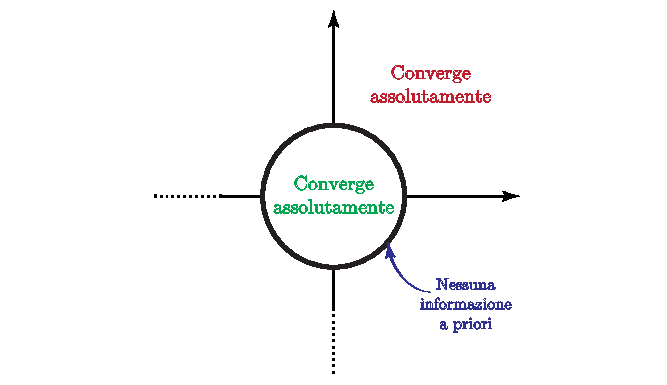
\includegraphics[trim=2.5cm 0.5cm 2.5cm 0cm, clip, scale=1]{images/discoconvergenza.pdf}
	\end{center}
\end{define}
Poiché sappiamo che la serie converge assolutamente per $\abs{z}<r$, lo studio del raggio di convergenza passa attraverso lo studio della serie assoluta associata $\displaystyle\sum_{n=0}^{+\infty}\abs{a_nz^n}$.\\
Per determinare il raggio di convergenza, possiamo ad esempio usare il \textbf{criterio di D’Alembert}\seeonlyindex{criterio!del rapporto}{criterio!di D’Alembert} o detto anche \textit{criterio del rapporto}\index{criterio!del rapporto}, che ci fornisce una condizione \textit{sufficiente} su come determinare il raggio di convergenza.
\begin{proposition}[Criterio di D’Alembert o del rapporto.]~{}\\
	Data la serie $\displaystyle\sum_{n=0}^{+\infty}a_nz^n$, se $a_n\neq 0$ definitivamente ed esiste il limite
	\begin{equation*}
		\lim_{n\to+\infty}\frac{\abs{a_{n+1}}}{\abs{a_{n}}}=L
	\end{equation*}
	allora
	\begin{enumerate}
		\item $L=0\implies R=+\infty$
		\item $L=+\infty\implies R=0$
		\item $0<L<+\infty\implies R=\frac{1}{L}$
	\end{enumerate}
\end{proposition}
Questa proposizione ha il vantaggio di essere operativamente utile, ma ovviamente solo se valgono le ipotesi: non è scontato che il limite del rapporto sia ben definito!\\
Un teorema più generale che vale \textit{per ogni serie} è il \textit{criterio della radice}\index{criterio!della radice} o altresì noto come \textbf{teorema di Cauchy-Hadamard}\seeonlyindex{criterio!del rapporto}{teorema!di Cauchy-Hadamard}.
\begin{theorema}[Teorema di Cauchy-Hadamard]~{}\\
	Sia data la serie di potenze
	\begin{equation*}
		\sum_{n=0}^{+\infty}a_nz^n
	\end{equation*}
	e sia
	\begin{equation}
		\lambda=\limsup_{n\to+\infty}\sqrt[n]{\abs{n}}
	\end{equation}
	Allora
	\begin{enumerate}
		\item Se $\lambda = 0$, la serie converge $\forall z\in\complexset$.
		\item Se $0<\lambda<+\infty$, la serie converge $R=\frac{1}{\lambda}$.
		\item Se $\lambda = +\infty$, la serie converge solo in $z=0$.
	\end{enumerate}

\end{theorema}
\begin{observe}
	I tre casi scritti esauriscono \textit{tutti} i casi possibili. Infatti, per la permanenza del segno del limsup\footnote{Nelle ‘‘Note aggiuntive'', a pagina XXX è possibile trovare la dimostrazione di questo risultato insieme ad altri relativi al limsup e liminf.} vale
	\begin{equation*}
		\sqrt[n]{\abs{a_n}}\geq 0,\ \forall n\geq 0\implies\limsup_{n\to+\infty}\sqrt[n]{\abs{a_n}}\geq 0
	\end{equation*}
\end{observe}
\begin{demonstration}\textsc{(del teorema di Cauchy-Hadamard.)}~{}\\
	Partiamo dal dimostrare il punto $2)$: dobbiamo provare che $R=\frac{1}{\lambda}$, ossia
	\begin{itemize}
		\item[a.] Se $\abs{z}<\nicefrac{1}{\lambda}$, allora $\displaystyle\sum_{n=0}^{+\infty}a_nz^n$ converge.
		\item[b.] Se $\abs{z}>\nicefrac{1}{\lambda}$, allora $\displaystyle\sum_{n=0}^{+\infty}a_nz^n$ \textit{non} converge.
	\end{itemize}
	La condizione (a.) infatti non basta per dimostrare che la convergenza è solo all'interno del cerchio. Proviamo ora le due tesi.
	\begin{itemize}
		\item[a.]	 Sia $z$ tale che $\abs{z}<\nicefrac{1}{\lambda}$. Se $z=0$ la serie banalmente converge perché ogni serie converge nel suo centro.\\
		Se $z\neq 0$, vale $\lambda<\nicefrac{1}{\abs{z}}$; consideriamo allora $\lambda'$ tale che $\lambda<\lambda'<\nicefrac{1}{\abs{z}}$: poiché $\lambda'>\lambda$, per la caratterizzazione del massimo limite si ha
		\begin{equation*}
			\textcolor{red}{\circled{\ast}}\quad\exists N\colon\forall n\geq N,\ \sqrt[n]{\abs{a_n}}<\lambda'
		\end{equation*}
		Proviamo che $\displaystyle\sum_{n=0}^{+\infty}a_nz^n$ converge assolutamente usando il criterio del confronto.
		\begin{equation*}
			\abs{a_nz^n}=\abs{a_n}\abs{z^n}=\abs{a_n}\abs{z}^n\substack{<}_{\textcolor{red}{\circled{\ast}}} \left(\lambda'\right)^n\abs{z}^n=\left(\lambda'\abs{z}\right)^n,\ \forall n\geq N
		\end{equation*}
		Questo è il termine $n$-esimo della serie geometrica $\displaystyle\sum_{n=0}^{+\infty}\left(\lambda'\abs{z}\right)^n$ di ragione $\lambda'\abs{z}$.\\
		Poiché $0<\lambda'\abs{z}<1$ per la scelta di $\lambda'$, la serie geometrica converge e quindi per il criterio del confronto converge anche la serie $\displaystyle\sum_{n=0}^{+\infty}\abs{a_nz^n}$ e dunque converge anche $\displaystyle\sum_{n=0}^{+\infty}a_nz^n$.
		\item[b.]	 Sia $z$ tale che $\abs{z}>\nicefrac{1}{\lambda}$. Per mostrare la non convergenza della serie proviamo che la condizione necessaria di convergenza non è soddisfatta, ovvero
		\begin{equation*}
			\lim_{n\to+\infty}a_nz^n\neq 0,\ \forall z\colon \abs{z}>\frac{1}{\lambda}
		\end{equation*}
		Per questo è sufficiente mostrare che
		\begin{equation*}
			\lim_{n\to+\infty}\abs{a_nz^n}\neq 0,\ \forall z\colon \abs{z}>\frac{1}{\lambda}
		\end{equation*}
		Notiamo che siamo passati da $\complexset$ a $\realset$ grazie alla norma, anche se in $\complexset$ ci trovavamo comunque in uno spazio metrico con la distanza indotta dal modulo.\\
		Poiché $z\neq 0$, vale $\lambda>\nicefrac{1}{\abs{z}}$.	Consideriamo allora $\lambda''$ tale che $\nicefrac{1}{\abs{z}}<\lambda''<\lambda$: poiché $\lambda''<\lambda$, per la caratterizzazione del massimo limite si ha
		\begin{equation*}
			\textcolor{blue}{\circled{\ast}}\quad\exists n_k\to+\infty\colon\sqrt[n_k]{\abs{a_{n_k}}}>\lambda''
		\end{equation*}
		Si ha, lungo la sottosuccessione:
		\begin{equation*}
			\abs{a_{n_k}z^{n_k}}=\abs{a_n}{z}^{n_k}\substack{>}_{\textcolor{blue}{\circled{\ast}}} \left(\lambda''\right)^{n_k}\abs{z}^{n_k}=\left(\substack{\lambda''\abs{z}>1}_{\text{ per la scelta di }\lambda''}\right)^{n_k}>1,\ \forall n_k
		\end{equation*}
		Poiché esiste una sottosuccessione che è sempre maggiore di $1$, deve esistere un valore limite della successione $\abs{a_nz^n}$ maggiore o uguale a $1$. Ma allora
		\begin{equation*}
			\limsup_{n\to+\infty}\abs{a_nz^n}\geq 1\implies\lim_{n\to+\infty}\abs{a_nz^n}\neq 0
		\end{equation*}
	\end{itemize}
	La dimostrazione del punto $1)$ è analoga alla prima parte della dimostrazione del punto $2)$. In questo caso, dobbiamo mostrare che la serie converge $\forall z\in\complexset$.\\ Se $z=0$, la serie banalmente converge, mentre se $z\neq 0$, si ha chiaramente che $0=\lambda<\nicefrac{1}{\abs{z}},\ \forall z\in\complexset\setminus\{0\}$. Consideriamo allora $\lambda'$ tale che $0<\lambda'<\nicefrac{1}{\abs{z}}$: poiché $\lambda'>0$, per la caratterizzazione del massimo limite si ha
	\begin{equation*}
		\textcolor{red}{\circled{\ast}}\quad\exists N\colon\forall n\geq N\ \sqrt[n]{\abs{a_n}}<\lambda'
	\end{equation*}
	Proviamo che $\displaystyle\sum_{n=0}^{+\infty}a_nz^n$ converge assolutamente usando il criterio del confronto.
	\begin{equation*}
		\abs{a_nz^n}=\abs{a_n}\abs{z^n}=\abs{a_n}\abs{z}^n\substack{<}_{\textcolor{red}{\circled{\ast}}} \left(\lambda'\right)^n\abs{z}^n=\left(\lambda'\abs{z}\right)^n,\ \forall n\geq N
	\end{equation*}
	Questo è il termine $n$-esimo della serie geometrica $\displaystyle\sum_{n=0}^{+\infty}\left(\lambda'\abs{z}\right)^n$ di ragione $\lambda'\abs{z}$.\\
	Poiché $0<\lambda'\abs{z}<1$ per la scelta di $\lambda'$, la serie geometrica converge e quindi per il criterio del confronto converge anche la serie $\displaystyle\sum_{n=0}^{+\infty}\abs{a_nz^n}$ e dunque converge anche $\displaystyle\sum_{n=0}^{+\infty}a_nz^n$. Poiché la scelta di $z$ è stata arbitraria, vale la tesi.\\
	La dimostrazione del punto $1)$ è analoga alla seconda parte della dimostrazione del punto $2)$. In questo caso, dobbiamo mostrare che la serie converge solo in $z=0$.\\ Se $z=0$, la serie banalmente converge. Per mostrare la non convergenza della serie proviamo che la condizione necessaria di convergenza non è soddisfatta, ovvero
	\begin{equation*}
		\lim_{n\to+\infty}a_nz^n\neq 0,\ \forall z\neq 0
	\end{equation*}
	Questo è equivalente a mostrare che
	\begin{equation*}
		\lim_{n\to+\infty}\abs{a_nz^n}\neq 0,\ \forall z\neq 0
	\end{equation*}
	Dato $z\neq 0$, consideriamo allora $\lambda''$ tale che $\nicefrac{1}{\abs{z}}<\lambda''<+\infty$: poiché $\lambda''<+\infty$, per la caratterizzazione del massimo limite si ha
	\begin{equation*}
		\textcolor{blue}{\circled{\ast}}\quad\exists n_k\to+\infty\colon\sqrt[n_k]{\abs{a_{n_k}}}>\lambda''
	\end{equation*}
	Si ha, lungo la sottosuccessione:
	\begin{equation*}
		\abs{a_{n_k}z^{n_k}}=\abs{a_n}{z}^{n_k}\substack{>}_{\textcolor{blue}{\circled{\ast}}}\left(\lambda''\right)^{n_k}\abs{z}^{n_k}=\left(\substack{\lambda''\abs{z}}_{>1\text{ per la scelta di }\lambda''}\right)^{n_k}>1,\ \forall n_k
	\end{equation*}
	Poiché esiste una sottosuccessione che è sempre maggiore di $1$, deve esistere un valore limite della successione $\abs{a_nz^n}$ maggiore o uguale a $1$. Ma allora
	\begin{equation*}
		\limsup_{n\to+\infty}\abs{a_nz^n}\geq 1\implies\lim_{n\to+\infty}\abs{a_nz^n}\neq 0
	\end{equation*}
	La scelta di $z$ è arbitraria, purché $z$ sia diverso da zero; per questo motivo vale la tesi.
\end{demonstration}
\section{Comportamento sul bordo}
Consideriamo la serie di potenze
\begin{equation*}
	\sum_{n=0}^{+\infty}a_nz^n,\quad a_n,\ z\in\complexset
\end{equation*}
con raggio di convergenza finito e non nullo.
I possibili comportamenti sul \textit{bordo} del cerchio di convergenza sono i seguenti:
\begin{enumerate}
	\item Convergenza in \textit{tutti i punti} del bordo del cerchio di convergenza
	\item \textit{Non} convergenza in \textit{nessun punto} del bordo del cerchio di convergenza
	\item Convergenza solo in \textit{alcuni punti} del bordo del cerchio di convergenza
\end{enumerate}
Mostriamo per ciascuno di essi un esempio.
\begin{example}\textsc{Caso 1.}~{}\\
	Consideriamo la serie
	\begin{equation*}
		\sum_{n=1}^{+\infty}\frac{z^n}{n^\alpha},\quad\alpha>1
	\end{equation*}
	Con la formula di D'Alembert vediamo che il raggio di convergenza è $R=1$. Infatti
	\begin{equation*}
		\lim_{n\to+\infty}\frac{\abs{a_{n+1}}}{\abs{a_{n}}}=\lim_{n\to+\infty}\frac{\left(n+1\right)^\alpha}{n^\alpha}=\lim_{n\to+\infty}\frac{n^\alpha\left(1+\frac{1}{n}\right)^\alpha}{n^\alpha}=\lim_{n\to+\infty}\left(1+\frac{1}{n}\right)^\alpha=1=\mathcal{l}\implies r=\frac{1}{\mathcal{l}}=1
	\end{equation*}
	Per ogni $z\in\complexset$ tale che $\abs{z}=1$ la serie converge (assolutamente):
	\begin{equation*}
		\sum_{n=1}^{+\infty}\abs{\frac{z^n}{n^\alpha}}=\sum_{n=1}^{+\infty}\frac{n}{n^\alpha}
	\end{equation*}
	La serie in modulo è la \textit{serie armonica generalizzata} che, per $\alpha>1$, converge; la serie semplice converge su tutti i punti del bordo.
\end{example}
\begin{example}\textsc{Caso 2.}~{}\\
	Consideriamo la \textit{serie geometrica}
	\begin{equation*}
		\sum_{n=1}^{+\infty}z^n
	\end{equation*}
	Poichè $a_n\equiv 1\ \forall n$, il criterio del rapporto ci fornisce come raggio di convergenza $R=1$.\\
	Per ogni $z\in\complexset$ tale che $\abs{z}=1$ la serie \textit{non} converge: possiamo osservare che presa la successione $c_n\in\complexset$, vale\footnote{Nelle ‘‘Note aggiuntive'', a pagina XXX è possibile trovare la dimostrazione di questo risultato.}
	\begin{equation*}
		\lim_{n\to+\infty}\abs{c_n}\neq 0\implies\lim_{n\to+\infty}c_n\neq 0
	\end{equation*}
	In questo caso:
	\begin{equation*}
		\lim_{n\to+\infty}\abs{z^n}=\lim_{n\to+\infty}1=1\neq 0\implies\lim_{n\to+\infty}z^n\neq 0
	\end{equation*}
	È evidente che la \textit{condizione necessaria} di convergenza \textit{non} è soddisfatta: la serie \textit{non} converge in nessun punto del bordo.
\end{example}
\begin{example}\textsc{Caso 3.}~{}\\
	Consideriamo la serie
	\begin{equation*}
		\sum_{n=1}^{+\infty}\frac{z^n}{n^\alpha},\quad0<\alpha<1
	\end{equation*}
	L'applicazione del criterio del confronto è esattamente analogo a quello visto nel caso  e il raggio di convergenza è pertanto $R=1$.\\
	Se $z=1$ la serie \textit{non} converge, dato che essa diventa una serie armonica generalizzata con $\alpha\leq1$:
	\begin{equation*}
		\sum_{n=1}^{+\infty}\frac{1}{n^\alpha}
	\end{equation*}
	Invece, per ogni $z\in\complexset$ tale che $\abs{z}=1$ e $z\neq 1$ la serie converge: infatti, possiamo applicare il \textit{criterio di Abel-Dirichlet}.
	\begin{equation*}
		\sum_{n=1}^{+\infty}\frac{z^n}{n^\alpha}=\sum_{n=1}^{+\infty}z^n\frac{1}{n^\alpha}=\sum_{n=1}^{+\infty}\alpha_n\beta_n
	\end{equation*}
	con $\alpha_n=z^n$ e $\beta_n=\nicefrac{1}{n^\alpha},\ n\geq 1$.
	\begin{enumerate}
		\item $\beta_n=\nicefrac{1}{n^\alpha}$ è una successione di elementi strettamente positivi, decrescenti e infinitesima per $n\to+\infty$.
		\item La successione delle \textit{somme parziali} di $\alpha_n=z^n$ è \textit{limitata}. Consideriamo
		\begin{equation*}
			\abs{\sum_{n=1}^{k}z^n}=\abs{\sum_{n=0}^{k}z^n-1}\squarequal
		\end{equation*}
		Poiché $\displaystyle\sum_{n=0}^{k}z^n$ è un serie geometrica parziale, sappiamo la sua somma parziale. Applicando poi una \textit{disuguaglianza triangolare}, troviamo una \textit{maggiorazione} della somma parziale di $\alpha_n$.
		\begin{equation*}
			\squarequal\abs{\frac{1-z^{k+1}}{1-z}-1}=\abs{\frac{z-z^{k+1}}{1-z}}\leq\frac{\abs{z}+\abs{-z^{k+1}}}{\abs{1-z}}\leq\frac{1+1}{\abs{1-z}}=\frac{2}{\abs{1-z}},\ \forall k\geq 1
		\end{equation*}
	\end{enumerate}
	Osserviamo che, nonostante la serie converga, essa non converge assolutamente: la serie in modulo è la serie armonica generalizzata con $\alpha\leq 1$, nota per essere divergente.
\end{example}
Anche se in generale non possiamo affermare a priori come converge sul bordo si può osservare che, in alcuni casi particolari, dalla convergenza in un punto del bordo si ottiene la convergenza sull'intero bordo. Vediamo alcuni risultati.
\begin{proposition}[Convergenza assoluta sul bordo se la serie di potenze converge assolutamente in un punto.]~{}\\
	Sia data la serie di potenze
	\begin{equation*}
		\sum_{n=1}^{+\infty}a_nz^n
	\end{equation*}
	Se la serie converge assolutamente in un punto della frontiera del cerchio di convergenza, allora converge assolutamente su tutta questa frontiera.
\end{proposition}
\begin{demonstration}
	Supponiamo che la serie converga assolutamente in $z_0$, dove $\abs{z_0}=R$ e prendiamo un qualunque $z$ tale che $\abs{z}=R$.
	Osserviamo che, presa la serie in modulo, si ha
	\begin{equation*}
		\sum_{n=1}^{+\infty}\abs{a_nz^n}=\sum_{n=1}^{+\infty}\abs{a_n}\abs{z^n}=\sum_{n=1}^{+\infty}\abs{a_n}\abs{z}^n=\sum_{n=1}^{+\infty}\abs{a_n}R^n=\sum_{n=1}^{+\infty}\abs{a_n}ì\abs{z_0}^n=\sum_{n=1}^{+\infty}\abs{a_nz_0^n}
	\end{equation*}
	che converge per ipotesi. Allora la serie di potenze converge assolutamente.
\end{demonstration}
\begin{corollary}[Convergenza sul bordo se la serie di potenze a coefficienti reali positivi converge in $z=R$.]~{}\\
	Sia data la serie di potenze
	\begin{equation*}
		\sum_{n=1}^{+\infty}a_nz^n
	\end{equation*}
	Se la serie ha coefficienti reali positivi e converge nel punto $z=R$, dove $R\in\left(0,+\infty\right)$ è il raggio di convergenza, allora converge in ogni punto della frontiera del cerchio di convergenza.
\end{corollary}
\begin{demonstration}
	Poiché $a_n$ e $R$ sono reali positivi, $a_n=\abs{a_n}$ e $R=\abs{R}$. Allora si ha
	\begin{equation*}
		\sum_{n=1}^{+\infty}a_nR^n=\sum_{n=1}^{+\infty}\abs{a_nR^n}
	\end{equation*}
	Quindi in questo caso la convergenza semplice della serie implica la convergenza assoluta. Poiché la serie converge assolutamente in un punto del bordo, segue dalla proposizione precedente la convergenza (assoluta) in tutti i punti del bordo.
\end{demonstration}
\section{Serie di potenze e convergenza uniforme}
\begin{theorema}[Converge uniforme delle serie di potenze.]~{}\\\label{convergenzasottoinsiemeH}
	Sia $\displaystyle\sum_{n=0}^{+\infty}a_nz^n$ una serie di potenze con raggio di convergenza $R\in\left(0,+\infty\right)$. Allora
	\begin{enumerate}
		\item La serie converge uniformemente su ogni insieme $H\subseteq\complexset$ tale che $\overline{H}\subsetneqq B_R\left(0\right)$, con $B_R\left(0\right)$ il disco aperto di convergenza, ovvero su qualsiasi insieme contenuto nel disco aperto tale che la sua chiusura non tocchi il bordo.
		\item Se la serie converge assolutamente in ogni $z\in\partial B_R\left(0\right)$ (il bordo del disco), allora converge uniformemente sul disco chiuso $\overline{B_R\left(0\right)}$.
	\end{enumerate}
\end{theorema}
\begin{demonstration} Per questa dimostrazione useremo il \textit{criterio di Weierstrass} enunciato nella sezione \ref{criteriodiweierstrass}, pag. \pageref{criteriodiweierstrass}.
	\begin{enumerate}
		\item Sia $H$ tale che $\overline{H}\subsetneqq B_R\left(0\right)$. Per il criterio di Weierstrass, per provare la convergenza uniforme su $H$ è sufficiente provare che esiste una successione $c_n$ tale che
		\begin{enumerate}
			\item $\abs{a_nz^n}\leq c_n,\ \forall z\in H$
			\item $\displaystyle\sum_{n=0}^{+\infty}c_n$ converge.
		\end{enumerate}
		\begin{minipage}{0.40\textwidth}
			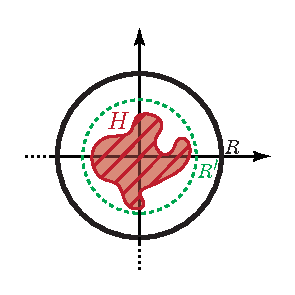
\includegraphics[trim=0cm 0cm 0cm 0cm, clip, scale=1]{images/discoconvergenzainsiemeH.pdf}
		\end{minipage}\hspace{-7mm}
		\begin{minipage}{0.55\textwidth}
			Poiché $H$ è solo \textit{strettamente contenuto} nel disco aperto di convergenza, $\exists R'<R$ tale che si abbia $\overline{H}\subseteq B_{R'}\left(0\right)$, ossia $\abs{z}\leq R',\ \forall z\in H$.\\
			Allora si ha, $\forall n\geq 0$ e $\forall z\in H$
			\begin{equation*}
				\abs{a_nz^n}=\abs{a_n}\abs{z}^n\leq \underbrace{\abs{a_n}\left(R'\right)^n}_{\text{$c_n$non dipende da }z}
			\end{equation*}
		\end{minipage}\\
		Inoltre, la serie $\displaystyle\sum_{n=0}^{+\infty}c_n=\sum_{n=0}^{+\infty}\abs{a_n}\left(R'\right)^n$ converge in quanto è la convergenza della serie di potenze per il punto $z=R'$, che è \textit{interno} al disco di convergenza $B_R\left(0\right)$. Applicando il criterio di Weierstrass otteniamo la tesi.
		\item Si ripete la dimostrazione sull'insieme $\overline{B_R\left(0\right)}$ con $R'=R$, considerando che la serie $\displaystyle\sum_{n=0}^{+\infty}\abs{a_n}R^n$ converge per ipotesi sulla convergenza sul bordo.
	\end{enumerate}
\end{demonstration}
\begin{example}\textsc{Serie geometrica.}\\
	Sulla \textit{serie geometrica} $\displaystyle\sum_{n=0}^{+\infty}z^n$ abbiamo già ricavato diverse informazioni: ha raggio di convergenza $R=1$ e \textit{non} c'è convergenza (assoluta) sul bordo, inoltre ne conosciamo la somma. Studiamo ora la convergenza uniforme.
	\begin{itemize}
		\item Converge uniformemente su ogni insieme $H$ tale che $\overline{H}\subsetneqq B_1\left(0\right)$ per il teorema precedente.
		\item Non avendo alcuna convergenza sul bordo, a priori non possiamo dare risultati generali sulla convergenza uniforme sulla base del teorema visto. Tuttavia, possiamo mostrare direttamente - grazie al fatto che la somma parziale e limite della serie geometrica è nota\footnote{Nelle ‘‘Note aggiuntive'', a pagina XXX è possibile trovare maggiori dettagli sulla somma (parziale) della serie geometrica e come ricavarla.} -  che la serie non converge uniformemente sul disco aperto $B_1\left(0\right)$. Infatti
		\begin{align*}
			\sup_{z\in B_1\left(0\right)}\abs{S_n\left(z\right)-S\left(z\right)}&=\sup_{z\in B_1\left(0\right)}\abs{\frac{1-z^{n+1}}{1-z}-\frac{1}{1-z}}=\sup_{z\in B_1\left(0\right)}\abs{\frac{-z^{n+1}}{1-z}}=\\
			&=\sup_{z\in B_1\left(0\right)}\frac{\abs{z}^{n+1}}{\abs{1-z}}=+\infty,\ \forall n\geq 0
		\end{align*}
		da cui
		\begin{equation*}
			\lim_{n\to+\infty}\left(\sup_{z\in B_1\left(0\right)}\abs{S_n\left(z\right)-S\left(z\right)}\right)=+\infty\neq 0
		\end{equation*}
	\end{itemize}
\end{example}
\section{Proprietà di regolarità della somma di una serie di potenze}
Sia $\displaystyle\sum_{n=0}^{+\infty}a_nz^n$ una serie di potenze con $R>0$ il raggio di convergenza. Studiamo le proprietà di continuità e derivabilità della \textbf{funzione somma}\index{funzione!somma}
\begin{equation}
	\funztot{f}{B_R\left(0\right)\subseteq\complexset}{\complexset}{z}{\displaystyle\sum_{n=0}^{+\infty}a_nz^n}
\end{equation}
\subsection{Continuità}
\begin{proposition}[Proprietà di continuità per la somma di una serie di potenze, caso generale.]~{}\\
	La funzione $f$ è continua su $B_R\left(0\right)$.
\end{proposition}
\begin{attention}
	La convergenza della serie di potenze su $B_R\left(0\right)$ \textit{non} è in generale uniforme, ma sappiamo al più che converge uniformemente su $H$ tale che $\overline{H}\subsetneqq B_R\left(0\right)$, quindi dobbiamo tenere conto di questo fattore nelle dimostrazioni che faremo.
\end{attention}
\begin{demonstration}
	Dobbiamo provare che $f\in\mathcal{C}\left(B_R\left(0\right)\right)$, cioè $f$ continua in $z_0,\ \forall z_0\in B_R\left(0\right)$. Sfrutto il fatto che la continuità è una proprietà locale, quindi fisso un punto e studio la continuità nel punto.\\	\vspace{3mm}
	\begin{minipage}{0.44\textwidth}
		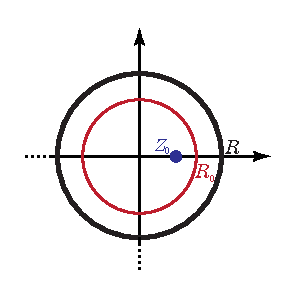
\includegraphics[trim=0cm 0cm 0cm 0cm, clip, scale=1.1]{images/discoconvergenzacontinuitaf.pdf}
	\end{minipage}\hspace{-9mm}
	\begin{minipage}{0.60\textwidth}
		Sia $z_0\in B_R\left(0\right)$ fissato. Per proprietà della metrica, allora $\exists R_0 < R$ tale che $z_0\in B_{R_0}\left(0\right)$. Su $B_{R_0}\left(0\right)$ si ha continuità uniforme e dunque, posto
		\begin{equation*}
			S_n\left(z\right)=\sum_{k=0}^{n}a_kz^k
		\end{equation*}
		si ha
		\begin{enumerate}
			\item $S_n$ continua su $B_{R_0}\left(0\right)$ perché è un polinomio.
			\item $S_n$ converge uniformemente a $f$ su $B_R\left(0\right)$.
		\end{enumerate}
	\end{minipage}\\
	Per il teorema di continuità della funzione limite, $f$ è continua in $B_{R_0}\left(0\right)$ e dunque in $z_0$. 
\end{demonstration}
%FINO A QUI
Questo risultato ci permette di parlare della convergenza sul disco aperto, ma se c'è qualche tipo di convergenza sul bordo, e quindi $f$ è definita anche su di esso, si può estendere la continuità di $f$ fino a tale frontiera? Studiamo due casi.
\begin{corollary}[Proprietà di continuità per la somma di una serie di potenze, caso sul bordo con convergenza assoluta.]~{}\\
	Sia data la serie di potenze $\displaystyle\sum_{n=0}^{+\infty}a_nz^n$ con raggio di convergenza $R>0$. Se la serie converge (assolutamente) su $\partial B_R\left(0\right)$ allora la serie è continua su $\overline{B_R\left(0\right)}$.
\end{corollary}
\begin{demonstration}
	Segue immediatamente ricordando che dalle ipotesi di convergenza assoluta sul bordo, sulla base del teorema \ref{convergenzasottoinsiemeH}, pag. \pageref{convergenzasottoinsiemeH}, vale la convergenza uniforme su $\overline{B_R\left(0\right)}$.
\end{demonstration}
Se invece supponiamo che la serie converga in un punto\footnote{Nel caso di più punti di convergenza $z_0,\ z_1,\ \ldots$, la funzione somma $f$ sarà definita su $B_R\left(0\right)\cup\left\{z_0\right\}\cup\left\{z_1\right\}\cup\ldots$. Qui riportiamo per semplicità il caso di un solo punto, ma i risultati successivi sono opportunamente generalizzabili con più punti di convergenza sul bordo.} $z_0$, cioè $\displaystyle\sum_{n=0}^{+\infty}a_nz_0^n$ converge, possiamo definire la \textbf{funzione somma}\index{funzione!somma} come
\begin{equation}
	\funztot{f}{B_R\left(0\right)\cup\left\{z_0\right\}\subseteq\complexset}{\complexset}{z}{\displaystyle\sum_{n=0}^{+\infty}a_nz^n}
\end{equation}
La convergenza uniforme di $f$ anche sui punti di convergenza $z_0$ sul bordo ci viene garantita dal \textbf{teorema di Abel}\index{teorema!di Abel}.
\begin{theorema}[Teorema di Abel.]~{}\\
	Sia dato la serie di potenze la serie di potenze $\displaystyle\sum_{n=0}^{+\infty}a_nz^n$ con raggio di convergenza $R>0$. Se $\exists z_0=Re^{i\theta_0}$ tale che $\displaystyle\sum_{n=0}^{+\infty}a_nz_0^n$ converge, allora\\
	\begin{minipage}{0.39\textwidth}
		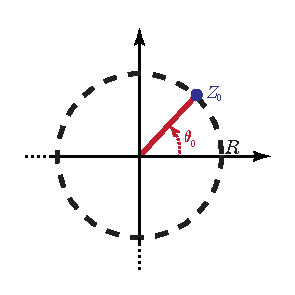
\includegraphics[trim=0cm 0cm 0cm 0cm, clip, scale=1]{images/discoconvergenzaabel.pdf}
	\end{minipage}\hspace{-12mm}
	\begin{minipage}{0.65\textwidth}
		\begin{enumerate}
			\item la serie converge uniformemente sul \textit{segmento}
			\begin{equation}
				\Sigma_0=\left\{z\in\complexset\mid z=re^{i\theta_0},\ r\in\left[0,R\right]\right\}
			\end{equation}
			\item La restrizione di $f$ a $\Sigma_0$ è \textit{continua} su $z_0$, ossia
			\begin{equation}
				\lim_{r\to R}f\left(re^{i\theta_0}\right)=f\left(z_0\right)=\sum_{n=0}^{+\infty}a_nz_0^n
			\end{equation}
		\end{enumerate}
	\end{minipage}
\end{theorema}
\subsection{Derivabilità}
Abbiamo definito la funzione somma dal disco aperto $B_R\left(0\right)$ in campo complesso a $\complexset$, ma al momento non conosciamo cosa vuol dire derivabilità di una funzione $\funz{f}{\complexset}{\complexset}$. Per il momento, limitiamoci al caso reale, cioè consideriamo una serie di potenze
\begin{equation*}
	\sum_{n=0}^{+\infty}a_nx^n,\ x\in\realset,\ a_n\in\realset
\end{equation*}
con raggio di convergenza $R>0$. In questo caso il cerchio di convergenza è un intervallo $\left(-R,R\right)$, con estremi eventualmente inclusi. La funzione somma risulta allora la funzione
\begin{equation}
	\funztot{f}{\left(-R,R\right)}{\realset}{x}{\sum_{n=0}^{+\infty}a_nx^n}
\end{equation}
\begin{theorema}[Derivabilità della somma di una serie di potenze.]~{}\\
	Sia data
	\begin{equation*}
		f\left(x\right)=\sum_{n=0}^{+\infty}a_nx^n,\ \forall x\in\left(-R,R\right),\ a_n\in\realset
	\end{equation*}
con $R>0$ il raggio di convergenza. Allora
\begin{enumerate}
	\item $f$ è derivabile su $\left(-R,R\right)$
	\item La derivata di $f$ è
	\begin{equation}
		f'\left(x\right)=\sum_{n=1}^{+\infty}na_nx^{n-1},\ \forall x\in\left(-R,R\right)
	\end{equation}
\end{enumerate}
\end{theorema}
Per dimostrare questo teorema useremo il teorema di derivibilità per serie di funzioni (teorema \ref{derivabilitatermineatermine}, pag. \pageref{derivabilitatermineatermine}, capitolo \refChapter{seriefunzioni}): poiché le ipotesi $1)$ e $2)$ sono banalmente verificate, dobbiamo contrarci sull'ipotesi $3)$, ovvero abbiamo bisogno di informazioni sulla convergenza uniforme della serie delle derivate $\displaystyle\sum_{n=1}^{+\infty}na_nx^{n-1}$; poiché la serie delle derivate è ancora una serie di potenze, allora ci basta studiare il raggio di convergenza.
% TO DO: nelle Note extra a pagina XXX inserire il prodotto del lim sup
\begin{lemming}[Convergenza della serie di derivate della serie di potenze.]~{}\\
	Sia data la serie di potenze $\displaystyle\sum_{n=0}^{+\infty}a_nx^n$ e sia $R>0$ il suo raggio di convergenza. Allora la serie di potenze $\displaystyle\sum_{n=1}^{+\infty}na_nx^{n-1}$ ha raggio di convergenza $R$.
\end{lemming}
\begin{demonstration}
	Riscriviamo la serie delle derivate, operando un cambio di indici ponendo $n=k+1$
	\begin{equation*}
		\sum_{n=1}^{+\infty}na_nx^{n-1}=\sum_{k=0}^{+\infty}\underbrace{\left(k+1\right)a_{k+1}}_{=b_k}x^k=\sum_{k=0}^{+\infty}b_ka_k
	\end{equation*}
	Sia $R'$ il suo raggio di convergenza. Per il teorema di Cauchy-Hadamard si ha
	\begin{equation*}
		\frac{1}{R'}=\limsup_{n\to+\infty}\abs{b_n}^{\nicefrac{1}{n}}=\limsup_{n\to+\infty}\abs{\left(n+1\right)a_{n+1}}^{\nicefrac{1}{n}}=\limsup_{n\to+\infty}\underbrace{\left(n+1\right)^{\nicefrac{1}{n}}}_{=\alpha_n}\underbrace{\abs{a_{n+1}}^{\nicefrac{1}{n}}}_{=\beta_n}=\limsup_{n\to+\infty}\alpha_n\beta_n\squarequal
	\end{equation*}
Osserviamo che
\begin{equation*}
	\lim_{n\to+\infty}\alpha_n=\lim_{n\to+\infty}\left(n+1\right)^{\nicefrac{1}{n}}=\lim_{n\to+\infty}e^{\frac{1}{n}\log\left(n+1\right)}=\lim_{n\to+\infty}e^{\frac{\log\left(n+1\right)}{n}}
\end{equation*}
Poichè $\frac{\log\left(n+1\right)}{n}\to 0$ per $n\to+\infty$ per confronto della crescita degli infiniti, $\displaystyle\lim_{n\to+\infty}\alpha_n=e^0=1$, dunque $\alpha_n$ ammette limite e dunque coincide col suo $\limsup$. Allora, per proprietà\footnote{Nelle ‘‘Note aggiuntive'', a pagina XXX è possibile trovare la dimostrazione di questo risultato insieme ad altri relativi al limsup e liminf.} del $\limsup$:
\begin{equation*}
	\squarequal\lim_{n\to+\infty}\alpha_n\limsup_{n\to+\infty}\beta_n=\limsup_{n\to+\infty}\abs{a_{n+1}}^{\nicefrac{1}{n}}=\limsup_{n\to+\infty}\left(\abs{a_{n+1}}^{\nicefrac{1}{n+1}}\right)^{\nicefrac{n+1}{n}}\squarequal
\end{equation*}
Poichè $\nicefrac{n+1}{n}\to 1$ per $n\to+\infty$, possiamo applicare Cauchy-Hadamar sulla serie di potenze $\displaystyle\sum_{n=0}^{+\infty}a_nx^n$ con raggio di convergenza $R>0$: poiché
\begin{equation*}
	\frac{1}{R}=\limsup_{n\to+\infty}\abs{a_n}^{\nicefrac{1}{n}}=\limsup_{n\to+\infty}\abs{a_{n+1}}^{\nicefrac{1}{n+1}}
\end{equation*}
allora abbiamo mostrato che
\begin{equation*}
	\frac{1}{R'}=\ldots=\limsup_{n\to+\infty}\left(\abs{a_{n+1}}^{\nicefrac{1}{n+1}}\right)^{\nicefrac{n+1}{n}}=\frac{1}{R}
\end{equation*}
cioè $R'=R$.
\end{demonstration}
Grazie a questo lemma, possiamo finalmente dimostrare il teorema lasciato in sospeso all'inizio della sezione.
\begin{demonstration}\textsc{(del Teorema di derivabilità della somma di una serie di potenze.)}\\
	Fissiamo $\overline{x}\in\left(-R,R\right)$ arbitrario e sia $\left(a,b\right)$ tale che
	\begin{itemize}
		\item $\overline{x}\in\left(a,b\right)$.
		\item $\left[a,b\right]\subsetneqq\left(-R,R\right)$
	\end{itemize}
Applichiamo ora il teorema di derivabilità termine a termine della serie di funzioni su $\left(a,b\right)$ sulla serie di potenze $\displaystyle\sum_{n=0}^{+\infty}a_nx^n$; vediamo che le ipotesi sono verificate:
\begin{itemize}
	\item $f_n\left(x\right)=a_nx^n$ derivabile in $\left(a,b\right),\ \forall n\geq 1$.
	\item $\displaystyle\sum_{n=0}^{+\infty}f_n\left(x\right)$ converge $\forall x\in\left(a,b\right)$
	\item $\displaystyle\sum_{n=1}^{+\infty}f'_n\left(x\right)=\sum_{n=1}^{+\infty}na_nx^{n-1}$ converge uniformemente su $\left(a,b\right)$ per la scelta di $\left(a,b\right)$, sulla base del lemma precedentemente dimostrato.
\end{itemize}
Per il teorema di derivabilità termine a termine $f$ è derivabile in $\left(a,b\right)$ e dunque anche in $\overline{x}$, con derivata in tal punto
\begin{equation*}
	f'\left(\overline{x}\right)=\sum_{n=1}^{+\infty}na_nx^{n-1}
\end{equation*}
Per l'arbitrarietà di $\overline{x}$, questi risultati valgono $\forall x\in\left(-R,R\right)$ e dunque segue la tesi.
\end{demonstration}
\section{Funzioni analitiche e serie di Taylor}
La tesi $2)$ appena dimostrata ci dice che la derivata $f'$ è una somma di serie di potenze con stesso raggio di convergenza $R$ di $f$. Possiamo riapplicare il teorema alla funzione $f'$:
\begin{itemize}
	\item $f'$ è derivabile in $\left(-R,R\right)$.
	\item $\displaystyle f''\left(x\right)=\sum_{n=2}^{+\infty}n\left(n-1\right)a_nx^{n-2},\ \forall x\in\left(-R,R\right)$.
\end{itemize}
Ma anche $f''$ è una serie di potenze con raggio $R$: possiamo riapplicare il teorema su $f''$ e ammettere l'esistenza di $f'''$ come serie di potenze. Iterando il ragionamento, si trova che esiste $f^{\left(k\right)}\left(x\right),\ \forall x\in\left(-R,R\right),\ \forall k\geq 0$ e vale
\begin{equation}
	f^{\left(k\right)}\left(x\right)=\sum_{n=k}^{+\infty}n\left(n-1\right)\ldots\left(n-k+1\right)a_nx^{n-k}=\sum_{n=k}^{+\infty}\frac{n!}{\left(n-k\right)!}a_nx^{n-k},\ \forall x\in\left(-R,R\right)
\end{equation}
Esplicitiamo il primo termine di $f^{\left(k\right)}\left(x\right)$:
\begin{align*}
	f^{\left(k\right)}\left(x\right)&=k\left(k-1\right)\ldots\left(k-k+1\right)a_kx^0+\sum_{n=k+1}^{+\infty}n\left(n-1\right)\ldots\left(n-k+1\right)a_nx^{n-k}=\\
	&=k!a_k+\sum_{n=k+1}^{+\infty}n\left(n-1\right)\ldots\left(n-k+1\right)a_nx^{n-k}
\end{align*}
In $x=0$ otteniamo
\begin{equation*}
	f^{\left(k\right)}\left(0\right)=k!a_k+0=k!a_k
\end{equation*}
Da cui otteniamo una espressione del termine $a_k$ in funzione della derivata $k$-esima, supponendo che esiste tale derivata:
\begin{equation}
	a_k=\frac{f^{\left(k\right)}}{k!},\ \forall k\geq 0
\end{equation}
Riscriviamo questi risultati in un unico teorema.
\begin{theorema}[Analiticità della somma di una serie di potenze.]~{}\\
	Sia data la serie di potenze
	\begin{equation*}
		\sum_{n=0}^{+\infty}a_nx^n,\ a_n\in\realset, x\in\realset
	\end{equation*}
con raggio di convergenza $R>0$ e sia $f$ la sua somma. Allora
\begin{enumerate}
	\item $f\in\mathcal{C}^{\infty}\left(\left(-R,R\right)\right)$.
	\item La derivata $k$-esima è nella forma
	\begin{equation}
		f^{\left(k\right)}\left(x\right)=\sum_{n=k}^{+\infty}n\left(n-1\right)\ldots\left(n-k+1\right)a_nx^{n-k}=\sum_{n=k}^{+\infty}\frac{n!}{\left(n-k\right)!}a_nx^{n-k},\ \forall x\in\left(-R,R\right)
	\end{equation}
	\item Il coefficiente $a_k$ si può scrivere come
	\begin{equation}
		a_k=\frac{f^{\left(k\right)}}{k!},\ \forall k\geq 0
	\end{equation}
	\item $f$ è \textit{analitica} in $0$, ossia si può scrivere come una \textbf{serie di Taylor di }$f$\textbf{centrata in }$x=0$\index{serie!di Taylor}
	\begin{equation}
		f\left(x\right)=\sum_{k=0}^{+\infty}\frac{f^{\left(k\right)}}{k!}x^k,\ \forall x\in\left(-R,R\right)
	\end{equation}
\end{enumerate}
\end{theorema}
Diamo una definizione formale del termine ‘‘funzione analitica'' che abbiamo appena usato nel teorema.
\begin{define}[Funzione analitica.]~{}\\
	Sia $\funz{f}{U\subseteq \realset}{\realset}$ tale che $f\in\mathcal{C}^{\infty}\left(U\right)$.
	\begin{enumerate}
		\item Dato $x_0\in\ U$, $f$ si dice \textbf{analitica}\index{analitica} in $x_0$ se $\exists r_0>0$ tale che
		\begin{equation*}
			f\left(x\right)=\sum_{k=0}^{+\infty}\frac{f^{\left(k\right)}\left(x_0\right)}{k!}\left(x-x_0\right)^k,\ \forall x\in\left(x_0-r_0,x_0+r_0\right)\subseteq U
		\end{equation*}
		\item f si dice \textbf{analitica in }$U$ se è analitica in ogni punto $x_0\in U$. In questo caso si scrive $f\in\mathcal{A}\left(U\right)$.
	\end{enumerate}
\end{define}
Il problema della \textit{ricostruzione} di una funzione come somma della sua serie di Taylor, introdotto nello studio della lunghezza dell'ellisse nel \refChapter{ellipseintroduction}, si può anche formulare come
\begin{center}
	‘‘Ogni funzione $f\in\mathcal{C}^{\infty}\left(U\right)$ è anche analitica su $U$?''
\end{center}
ossia
\begin{equation*}
	f\in\mathcal{C}^{\infty}\left(U\right)\stackrel{?}{\implies}f\in\mathcal{A}\left(U\right)
\end{equation*}
In generale la risposta è \textbf{no}, come possiamo vedere nell'esempio successivo.
\begin{example}
	Consideriamo la funzione
	\begin{equation*}
		f\left(x\right)=
		\begin{cases}
			\begin{array}{ll}
				e^{-\frac{1}{x^2}}&\text{se }x\neq 0\\
				0&\text{se }x=0
			\end{array}
		\end{cases}
	\end{equation*}
$f$ è certamente di classe $\mathcal{A}^{\infty}\left(\realset\setminus\left\{0\right\}\right)$; si verifica che esiste $f^{\left(k\right)}=0,\ \forall k\geq 0$ e che $f^{\left(k\right)}\in\mathcal{C}\left(\realset\right),\ \forall k\geq 0$, dunque $f\in\mathcal{C}\left(\realset\right)$:\\
Tuttavia, $f\notin\mathcal{A}\left(\realset\right)$. Infatti, la serie di Taylor centrata in $x_0=0$ è
\begin{equation*}
	\sum_{k=0}^{+\infty}\frac{f^{\left(k\right)}\left(0\right)}{k!}x^k=\sum_{k=0}^{+\infty}\frac{0}{k!}x^k\equiv 0
\end{equation*}
che converge ma \textit{non} a $f$, ossia $f\left(x\right)\neq 	\sum_{k=0}^{+\infty}\frac{f^{\left(k\right)}\left(0\right)}{k!}x^k,\ \forall x\neq 0$.
\end{example}
% TO DO: controesempio su moodle
Bisogna quindi capire sotto quali ipotesi ulteriori una funzione di classe $\mathcal{C}^{\infty}$ è anche analitica; cerchiamo a tal scopo una condizione \textit{sufficiente}.\\
Riprendiamo il problema come era stato posto originalmente; approssimiamo $f$ con il \textit{polinomio} di Taylor, tenendo conto del \textit{resto} $R_n\left(x\right)$:
\begin{equation*}
	f\left(x\right)=\sum_{k=0}^{n}\frac{f^{\left(k\right)}\left(x_0\right)}{k!}\left(x-x_0\right)^k+R_n\left(x\right)
\end{equation*}
Per passare da questa approssimazione alla riscrittura di $f$ come \textit{serie} di Taylor è necessario ridurre il resto dell'approssimazione a zero al crescere dei termini del polinomio, ossia
\begin{equation*}
	\lim_{n\to+\infty}R_n\left(x\right)=0
\end{equation*}
Ricordiamo l'espressione del resto in \textit{forma di Lagrange}:
\begin{equation*}
	\exists \xi=\xi_{x,n}\colon R_n\left(x\right)=\frac{f^{\left(n+1\right)}\left(\xi\right)}{\left(n+1\right)!}\left(x-x_0\right)^{n+1}
\end{equation*}
La condizione sufficiente che andremo ora a definire necessita di avere una informazione sulle derivate $f^{\left(n\right)}$ per $n$ \textit{sufficientemente grande}.
\begin{theorema}[Condizione sufficiente di analiticità.]~{}\\\label{condizionesufficienteanaliticita}
	Sia $\funz{f}{U\subseteq\realset}{\realset}$, $f\in\mathcal{C}^{\infty}\left(U\right)$ e sia $x_0\in U$. Se $\exists r_0>0,\ \exists M>0,\ \exists n_0>0$ tale che
	\begin{equation}
		\abs{f^{\left(n\right)}\left(x\right)}\leq\frac{Mn!}{r_0^n},\ \forall x\in\left(x_0-r_0,x_0+r_0\right),\ \forall n\geq n_0
	\end{equation}
	allora $f$ è \textit{analitica} in $x_0$ e vale
	\begin{equation*}
		f\left(x\right)=\sum_{k=0}^{+\infty}\frac{f^{\left(k\right)}\left(x_0\right)}{k!}\left(x-x_0\right)^k,\ \forall x\in\left(x_0-r_0,x_0+r_0\right)
	\end{equation*}
\end{theorema}
\begin{demonstration}
	Sia $x\in\left(x_0-r_0,x_0+r_0\right)$ fissato. Dobbiamo provare che
	\begin{equation*}
		\lim_{n\to+\infty}R_n\left(x\right)=\lim_{n\to+\infty}\frac{f^{\left(n+1\right)}\left(\xi\right)}{\left(n+1\right)!}\left(x-x_0\right)^{n+1}=0
	\end{equation*}
dove $\xi$ è ottenuto applicando la formula di Taylor con il resto in \textit{formula di Lagrange}. Poiché $\xi\in\left(x_0-r_0,x_0+r_0\right)$, per l'ipotesi di partenza si può stimare $f^{\left(n+1\right)}\left(\xi\right)$:
\begin{align*}
	0\leq \abs{\frac{f^{\left(n+1\right)}\left(\xi\right)}{\left(n+1\right)!}\left(x-x_0\right)^{n+1}}&=\frac{\abs{f^{\left(n+1\right)}\left(\xi\right)}}{\left(n+1\right)!}\abs{x-x_0}^{n+1}\stackrel{\leq}{\forall n\geq n_0}\frac{\frac{M\Ccancel[red]{\left(n+1\right)!}}{r_0^{n+1}}}{\Ccancel[red]{\left(n+1\right)!}}\abs{x-x_0}^{n+1}=\\
	&=M\frac{\abs{x-x_0}^{n+1}}{r_0^{n+1}}=M\left(\frac{\abs{x-x_0}}{r_0}\right)^{n+1}
\end{align*}
Abbiamo quindi ottenuto
\begin{equation*}
	0\leq \abs{R_n\left(x\right)}\leq M\left(\frac{\abs{x-x_0}}{r_0}\right)^{n+1},\ \forall n\geq n_0
\end{equation*}
Poiché $\left(\frac{\abs{x-x_0}}{r_0}\right)^{n+1}$ è una successione geometrica di ragione $\frac{\abs{x-x_0}}{r_0}\in\left(0,1\right)$, essa tende a $0$ per $n\to+\infty$: per il teorema del confronto abbiamo $\displaystyle\lim_{n\to+\infty}R_n\left(x\right)=0$.
\end{demonstration}
\begin{observe}\label{condizionesufficientederivatelimitate}
	Questa condizione sufficiente si verifica anche se $\exists M>0, \exists r_0>0$ tale per cui
	\begin{equation*}
		\abs{f^{\left(n\right)}\left(x\right)}\leq M,\ \forall x\in\left(x_0-r_0,x_0+r_0\right),\ \forall n\geq 0
	\end{equation*}
Infatti, $\forall r_0>0$, per confronto di crescita si ha
\begin{equation*}
	\lim_{n\to+\infty}\frac{n!}{r_0^n}=+\infty
\end{equation*}
Dunque esiste sempre $n_0$ tale che $\forall n\geq n_0$ si ha $\frac{n!}{r_0^n}>1$. Segue allora
\begin{equation*}
	\abs{f^{\left(n\right)}\left(x\right)}\leq M<M\frac{n!}{r_0^n},\ \forall x\in\left(x_0-r_0, x_0+r_0\right),\ \forall n\geq n_0
\end{equation*}
\end{observe}
\section{Esempi di funzioni analitiche}
\begin{theorema}[Analiticità di {$e^x$}, {$\cos x$}, {$\sin x$}, {$\left(1+x\right)^\alpha$}.]~{}\\
	Le funzioni $e^x$, $\cos x$, $\sin x$, $\left(1+x\right)^\alpha$ con $\alpha\in\realset$ sono analitiche in $x_0=0$ e vale
	\begin{align}
		e^x&=\sum_{k=0}^{+\infty}\frac{1}{k!}x^k,\ \forall x\in\realset\\
		\sin x&=\sum_{k=0}^{+\infty}\frac{\left(-1\right)^k}{\left(2k\right)!}x^{2k},\ \forall x\in\realset\\
		\cos x&=\sum_{k=0}^{+\infty}\frac{\left(-1\right)^k}{\left(2k+1\right)!}x^{2k+1},\ \forall x\in\realset\\
		\left(1+x\right)^\alpha&=\sum_{k=0}^{+\infty}\binom{\alpha}{k}x^k,\ \forall x\in\left(-1,1\right),\ \forall \alpha\in\realset
	\end{align}
\end{theorema}
\begin{attention}
	L'ultima formula vale solo per $x\in\left(-1,1\right)$, indipendentemente dal dominio di $\left(1+x\right)^\alpha$. Ad esempio, se $\alpha=\frac{1}{3}$, $\left(1+x\right)^\alpha=\sqrt[3]{1+x}$ è definita su tutto $\realset$, però si può scrivere somma della sua serie di Taylor solo in $\left(-1,1\right)$; in altre parole, l'analiticità è una proprietà \textit{locale}.
\end{attention}
Le prime tre formule si dimostrano usando la condizione sufficiente precedentemente dimostrata. Per quanto riguarda la quarta formula, \textit{non} si riesce a verificare la validità di tale condizione, ma con un altro ragionamento si trova comunque l'analiticità. Questo mostra che la condizione scritta sopra è \textit{solo} sufficiente, ma \textit{non} necessaria per l'analiticità.
\begin{demonstration}~{}
	\begin{itemize}
		\item $e^x$, $\sin x$, $\cos x$. È noto che
		\begin{equation*}
			\sum_{k=0}^{n}\frac{1}{k!}x^k\quad\sum_{k=0}^{n}\frac{\left(-1\right)^k}{\left(2k\right)!}x^{2k}\quad\sum_{k=0}^{n}\frac{\left(-1\right)^k}{\left(2k+1\right)!}x^{2k+1}
		\end{equation*}
		sono i polinomi di Taylor di $e^x,\ \cos x$ e $\sin x$ centrati in $x_0=0$. Per $n\to+\infty$ si ottengono le serie di Taylor
		\begin{equation*}
			\sum_{k=0}^{+\infty}\frac{1}{k!}x^k\quad\sum_{k=0}^{+\infty}\frac{\left(-1\right)^k}{\left(2k\right)!}x^{2k}\quad\sum_{k=0}^{+\infty}\frac{\left(-1\right)^k}{\left(2k+1\right)!}x^{2k+1}
		\end{equation*}
	Proviamo ora che valgono le uguaglianze scritte. Per dimostrare che valgono su tutto $\realset$ è sufficiente dimostrate che valgono su un intervallo del tipo $\left(-r_0, r_0\right)$ con $r_0>0$ arbitrario.\\
	Sia allora $r_0>0$ fissato arbitrariamente e sia $x\in\left(-r_0, r_0\right)$. Proviamo che è vera la condizione a pag. \pageref{condizionesufficientederivatelimitate}, che sappiamo implicare la condizione sufficiente a pag. \pageref{condizionesufficienteanaliticita}. Vediamo i tre casi:
	\begin{itemize}
		\item $e^x$. La derivata di $f\left(x\right)=e^x$ è $f^{\left(n\right)}\left(x\right)=e^x$, quindi si ha
		\begin{equation*}
			\abs{f^{\left(n\right)}\left(x\right)}=e^x\leq e^{r_0}= M,\ \forall x\in\left(-r_0,r_0\right),\ \forall n\geq 0
		\end{equation*}
		\item $\cos x$, $\sin x$. Poiché le derivate di seno e coseno sono ciclicamente seno e coseno con opportuni segni, la derivata $n$-esima di $\cos x$ e $\sin x$ in modulo è sempre limitata da 1.
		\begin{equation*}
			\abs{f^{\left(n\right)}\left(x\right)}\leq 1 = M,\ \forall x\in\left(-r_0,r_0\right),\ \forall n\geq 0
		\end{equation*}
	\end{itemize}
	Poiché la condizione è verificata su $\left(-r_0,r_0\right)$ e vale l'analiticità su tale intervallo, per l'arbitrarietà di $r_0$ l'analiticità si verifica su tutto $\realset$.
	\item $\left(1+x\right)^\alpha$. Mostriamo innanzitutto che la serie di potenze $\displaystyle\sum_{n=0}^{+\infty}\binom{\alpha}{k}x^k$ converge $\forall x\in\left(-1,1\right)$, usando il criterio del rapporto:
	\begin{align*}
		R&=\lim_{n\to+\infty}\frac{\abs{a_n}}{\abs{a_{n+1}}}=\lim_{n\to+\infty}\frac{\abs{\alpha\left(\alpha-1\right)\ldots\left(\alpha-n+1\right)}}{n!}\frac{\left(n+1\right)!}{|\alpha\left(\alpha-1\right)\underbrace{\left(\alpha-\left(n+1\right)+1\right)}_{\alpha-n}|}=\\
		&=\lim_{n\to+\infty}\frac{\abs{n+1}}{\abs{\alpha-n}}=\lim_{n\to+\infty}\frac{n+1}{n-\alpha}=1
	\end{align*}
	Adesso definiamo la funzione somma
	\begin{equation*}
		g_\alpha\left(x\right)=\sum_{n=0}^{+\infty}\binom{\alpha}{n}x^n,\ \forall x\in\left(-1,1\right)
	\end{equation*}
	Dobbiamo dimostrare che $g_\alpha\left(x\right)=\left(1+x\right)^{\alpha},\ \forall x\in\left(-1,1\right)$. Per la derivazione termine a termine abbiamo
	\begin{align*}
		g'_\alpha\left(x\right)&=\sum_{n=1}^{+\infty}n\binom{\alpha}{n}x^{n-1}=\sum_{n=1}^{+\infty}\frac{\alpha\left(\alpha-1\right)\ldots\left(\alpha-n+1\right)}{n!}nx^{n-1}=\\
		&=\alpha\sum_{n=1}^{+\infty}\frac{\left(\alpha-1\right)\ldots\left(\alpha-1\left(n-1\right)+1\right)}{\left(n+1\right)!}x^{n-1}=\alpha\sum_{n=1}^{+\infty}\binom{\alpha-1}{n-1}x^{n-1}=\\
		&\underrel[c]{n-1=m}{=}\alpha\sum_{m=0}^{+\infty}\binom{\alpha-1}{m}x^m=\alpha g_{\alpha-1}\left(x\right),\ \forall x\in\left(-1,1\right)
	\end{align*}
	Quindi $g'_{\alpha}\left(x\right)=\alpha g_{\alpha-1}\left(x\right),\ \forall x\in\left(-1,1\right)$. Osserviamo che
	\begin{align*}
		\left(1+x\right)g_{\alpha-1}\left(x\right)&=\sum_{n=0}^{+\infty}\binom{\alpha-1}{n}x^n+\sum_{n=0}^{+\infty}\binom{\alpha-1}{n}x^{n+1}=\\
		&\underrel{n+1=m}{=}\sum_{n=0}^{+\infty}\binom{\alpha-1}{n}x^n+\sum_{m=1}^{+\infty}\binom{\alpha-1}{m-1}x^{m}=\\
		&=1+\sum_{m=1}^{+\infty}\left[\binom{\alpha-1}{m}+\binom{\alpha-1}{m-1}\right]x^m=1+\sum_{m=1}^{+\infty}\binom{\alpha}{m}x^m
	\end{align*}
	Infatti, si ha
	\begin{align*}
		\binom{\alpha-1}{m}+\binom{\alpha-1}{m-1}&=\frac{\left(\alpha-1\right)\left(\alpha-2\right)\ldots\left(\alpha-1-m+1\right)}{m!}+\frac{\left(\alpha-1\right)\left(\alpha-2\right)\ldots\left(\alpha-1-\left(m-1\right)+1\right)}{\left(m-1\right)!}=\\
		&=\frac{\left(\alpha-1\right)\left(\alpha-2\right)\ldots\left(\alpha-1-\left(m-1\right)+1\right)}{\left(m-1\right)!}\frac{\left(\alpha\Ccancel[red]{-1-m+1+m}\right)}{m}=\frac{\alpha\left(\alpha-1\right)}{m}=\\
		&=\frac{\alpha\left(\alpha-1\right)\ldots\left(\alpha-m+1\right)}{m!}=\binom{\alpha}{m}
	\end{align*}
Riassumendo, abbiamo ottenuto che
\begin{equation*}
	\left(1+x\right)g_{\alpha-1}\left(x\right)=g_\alpha\left(x\right)
\end{equation*}
Si ha
\begin{equation*}
	\begin{cases}
		g'_{\alpha}\left(x\right)=\frac{\alpha}{\left(1+x\right)}g_{\alpha}\left(x\right)\\
		g_{\alpha}\left(0\right)=1
	\end{cases}
\end{equation*}
che è un \textit{problema di Cauchy} o altresì noto come un'\textit{equazione differenziale lineare} omogenea del I grado con dato iniziale, la cui soluzione è
\begin{equation*}
	g_{\alpha}\left(x\right)=e^{\alpha\int_{0}^{x}\frac{1}{1+t}dt}=e^{\alpha\log\left(1+x\right)}=\left(1+x\right)^{\alpha},\ \forall x\in\left(-1,1\right)
\end{equation*}
\end{itemize}
\end{demonstration}
\begin{digression}\textsc{\textbf{Uno sguardo al futuro: il caso complesso}}\\
	In \textsc{Analisi Matematica 4} si riprenderà la questione della derivabilità in campo complesso, definendola e proseguendo con il problema di studiare l'analiticità delle funzioni in campo complesso.\\
	Se in campo reale le funzioni \textit{analitiche} sono solo un piccolo sottoinsieme delle funzioni $\mathcal{C}^{\infty}\left(U\right)$, a loro volta un sottoinsieme stretto delle funzioni $\mathcal{C}^1\left(U\right),\ \mathcal{C}^2\left(U\right),\ \ldots$, a loro volta sottoinsieme delle funzioni \textit{derivabili} $D\left(U\right)$ e infine delle funzioni \textit{continue} $\mathcal{C}\left(U\right)$.\\
	% TO DO: disegnare insieme di Eulero-Venn delle funzioni reali
	In campo complesso abbiamo una sorpresa. Infatti, se la funzione è \textit{derivabile} una volta, lo è \textit{infinitamente} con continuità e sono anche \textit{analitiche}!
	\begin{equation*}
		D\left(U\right)=\mathcal{C}^1\left(U\right)=\ldots=\mathcal{C}^{\infty}\left(U\right)=\mathcal{A}
	\end{equation*}
\end{digression}
\section{Funzioni esponenziale e logaritmo in campo complesso}
\subsection{Funzione esponenziale in campo complesso}
\begin{define}[Esponenziale in campo complesso.]~{}\\
	L'\textbf{esponenziale in campo complesso}\index{esponenziale!in campo complesso} è la funzione definita $\forall z\in\complexset$ come
	\begin{equation}
		e^z\coloneqq\sum_{n=0}^{+\infty}\frac{z^n}{n!}
	\end{equation}
\end{define}
\begin{demonstration}
	Questa funzione è ben definita. Applichiamo alla serie di potenze $\displaystyle \sum_{n=0}^{+\infty}\frac{z^n}{n!}$ il criterio di d'Alembert:
	\begin{equation*}
		\lim_{n\to+\infty}\frac{\frac{1}{\left(n+1\right)!}}{\frac{1}{n!}}=\lim_{n\to+\infty}\frac{n!}{\left(n+1\right)!}=\lim_{n\to+\infty}\frac{1}{n+1}=0
	\end{equation*}
Segue che converge per ogni $z\in\complexset$.
\end{demonstration}
\begin{observe}
	Ricordando che in campo reale vale la relazione
	\begin{equation*}
		e^z=\sum_{n=0}^{+\infty}\frac{x^n}{n!},\ \forall x\in\realset
	\end{equation*}
	si ricava che la funzione esponenziale definita in campo complesso coincide con la nota funzione esponenziale nel caso di $z=x\in\realset$.
\end{observe}
\begin{proposition}[Proprietà dell'esponenziale complesso.]~{}
	\begin{enumerate}
		\item $e^{z_1+z_2}=e^{z_1}e^{z_2},\ \forall z_1,\ z_2\in\complexset$
		\item $e^z\neq 0,\ \forall z\in\complexset$.
		\item $e^{-z}=\frac{1}{e^z},\ \forall z\in\complexset$.
		\item Vale la \textbf{formula di Eulero}\index{formula!di Eulero}:
		\begin{equation}
			e^{iy}=\cos y+i\sin y,\ \forall y\in\realset
		\end{equation}
		\item $e^{x+iy}=e^{x}\left(\cos y+i\sin y\right),\ \forall x,y\in\realset$.
		\item $\abs{e^z}=e^{\Re z},\ \arg\left(e^z\right)=\Im z+2k\pi,\ k\in\integerset,\ \forall z\in\complexset$.
		\item $e^{z+2k\pi i}=e^z,\ \forall z\in\complexset, k\in\integerset$.
	\end{enumerate}
\end{proposition}
\begin{demonstration}~{}\\
\begin{enumerate}[label=\Roman*]
\item Siano $z_1,\ z_2\in\complexset$. Dobbiamo provare che
\begin{equation*}
	\sum_{n=0}^{+\infty} \frac{(z_1+z_2)^n}{n!} =\sum_{n=0}^{+\infty} \frac{z_1^n}{n!} \cdot \sum_{n=0}^{+\infty} \frac{z_2^n}{n!}
\end{equation*}
Ricordiamo\footnote{Nelle ‘‘Note aggiuntive'', a pagina \ref{prodottosecondocauchy} è possibile trovare alcune informazioni sulla proprietà di prodotto (secondo Cauchy).} che, date due serie
\begin{equation*}
	\sum_{n=0}^{+\infty} \alpha_n,\quad \sum_{n=0}^{+\infty} \beta_n,\quad \alpha_n, \ \beta_n \in \complexset
\end{equation*}
il loro prodotto è la serie
\begin{equation*}
	\sum_{n=0}^{+\infty} \gamma_n,\ \text{dove }\gamma_n= \sum_{k=0}^{n} \alpha_k\ \beta_{n-k},\quad \forall \ n\geq 0
\end{equation*}
Nel caso in questione $\alpha_n=\frac{z_1^n}{n!},\quad \beta_n = \frac{z_2^n}{n!},\quad \forall \ n\geq 0$, dunque
\begin{equation*}
	\gamma_n= \sum_{k=0}^{n} \frac{z_1^k}{k!}\ \frac{z_2^{(n-k)}}{(n-k)!}=\sum_{k=0}^{n} \frac{z_1^k\, z_2^{(n-k)}}{k!(n-k)!},\quad \forall \ n\geq 0.
\end{equation*}
Osserviamo che vale
\begin{equation*}
	\frac{1}{k!(n-k)!}= \frac{1}{n!}\binom{n}{k},\quad \forall \ n\geq 0,\ 0\leq k\leq n.
\end{equation*}
Dalla formula del binomio di Newton, ricaviamo allora
\begin{equation*}
	\gamma_n= \sum_{k=0}^{n} \frac{z_1^k}{k!}\ \frac{z_2^{(n-k)}}{(n-k)!}=\frac{1}{n!}\, \sum_{k=0}^{n} \binom{n}{k}\, z_1^k\, z_2^{(n-k)} =\frac{(z_1+z_2)^n}{n!},\quad \forall \ n\geq 0
\end{equation*}
Abbiamo quindi ottenuto la tesi:
\begin{equation*}
	\sum_{n=0}^{+\infty} \frac{z_1^n}{n!} \cdot \sum_{n=0}^{+\infty} \frac{z_2^n}{n!}= \sum_{n=0}^{+\infty} \frac{(z_1+z_2)^n}{n!}
\end{equation*}
\item[I--III] Sia $z\in\complexset$ fissato. Applichiamo la formula dimostrata al punto I con $z_1=z$ e $z_2=-z$; otteniamo
\begin{equation*}
	e^{z-z}  = e^{z}e^{-z}\implies 1 = e^{z}e^{-z}
\end{equation*}
Da questo segue che $e^{-z} = \nicefrac{1}{e^z}$.
\item[IV] Fissato $y\in\realset$, dalla definizione dell'esponenziale complesso segue che
\begin{equation*}
	e^{iy}=\sum_{n=0}^{+\infty}\frac{\left(iy\right)^n}{n!}=\sum_{n=0}^{+\infty}\frac{i^ny^n}{n!}
\end{equation*}
Riordiniamo i termini della serie separando i termini di posto pari e quelli di posto dispari\footnote{Per riordinare la serie come due ‘‘sottoserie'' senza che la somma venga modificata è necessaria la convergenza assoluta. Poiché ogni serie di potenze converge assolutamente all'interno del suo cerchio di convergenza, in questo caso non abbiamo problemi di riorganizzazione della serie. Nelle ‘‘Note aggiuntive'', a pagina XXX è possibile trovare alcune informazioni sul problema di riorganizzazione della serie.}, ottenendo
\begin{equation*}
	e^{iy}=\sum_{n=0}^{+\infty}\frac{i^{2k}y^{2k}}{\left(2k\right)!}+\sum_{n=0}^{+\infty}\frac{i^{2k+1}y^{2k+1}}{\left(2k+1\right)!}
\end{equation*}
Calcoliamo ora $i^{2k}$ e $i^{2k+1}$:
\begin{itemize}
	\item $i^{2k}=\left(i^2\right)^k=\left(-1\right)^k$.
	\item $i^{2k+1}=i\left(i^2\right)^k=i\left(-1\right)^k$.
\end{itemize}
Allora
\begin{equation*}
	e^{iy}=\sum_{n=0}^{+\infty}\frac{\left(-1\right)^ky^{2k}}{\left(2k\right)!}+i\sum_{n=0}^{+\infty}\frac{\left(-1\right)^ky^{2k+1}}{\left(2k+1\right)!}
\end{equation*}
Ricordando che
\begin{equation*}
	\cos y=\sum_{n=0}^{+\infty}\frac{\left(-1\right)^ky^{2k}}{\left(2k\right)!}\quad
	\sin y=\sum_{n=0}^{+\infty}\frac{\left(-1\right)^ky^{2k+1}}{\left(2k+1\right)!}
\end{equation*}
segue la tesi.
\item[V] Sia $z=x+iy$, con $x,y\in\realset$. Dalla relazione provata in I segue che $e^{x+iy}=e^xe^{iy}$. Applicando la \textit{formula di Eulero}, si ha la tesi.
\item[VI] Sia $z=x+iy$, con $x,y\in \realset$, ossia $x=\Re z e y=\Im z$. 
La formula provata al punto V esprime il numero complesso $e^z$ in forma trigonometrica; da essa si ricava quindi immediatamente il risultato.
\item[VII]  Siano $z\in \complexset$ e $k\in \integerset$. Dalla relazione provata al punto I segue che 
\begin{equation*}
	e^{z+2k\pi i}=e^{z}\, e^{2k\pi i}
\end{equation*}
Applicando la \textbf{formula di Eulero} si ricava immediatamente che 
\begin{equation*}
	e^{2k\pi i}=\cos 2k\pi +i\sin 2k\pi =1
\end{equation*}
e questo consente di concludere la tesi.
\end{enumerate}
\end{demonstration}
\begin{observe}
	Dalla relazione $e^{z+2k\pi i}=e^z,\ \forall z\in\complexset, k\in\integerset$ segue che in campo complesso la funzione esponenziale è \textbf{periodica} di periodo $2\pi i$.\\
	% TO DO: disegnare numeri complessi con lo stesso esponenziale
	Di conseguenza, in campo complesso la funzione esponenziale \textit{non} è invertibile.\\
	L'\textit{invertibilità} è però garantita consentendo come inversa una \textit{funzione multivoca}.
\end{observe}
\begin{define}[Funzione multivoca.]~{}\\
	Una \index{funzione!multivoca} è una \textit{relazione binaria seriale} che associa ad ogni valore $x$ nel dominio $X$ uno o più valori $y$ nel codominio $Y$.
\end{define}
\subsection{Funzione logaritmo in campo complesso}
\begin{define}[Logaritmo in campo complesso.]~{}\\
	Dato un numero complesso $z$, si chiamano \textbf{logaritmi complessi} di $z$, se esistono, i numeri complessi $w$ tali che
	\begin{equation}
		e^w=z
	\end{equation}
	L'insieme di tali numeri si indica con
	\begin{equation}
		\log z
	\end{equation}
\end{define}
Proviamo ora che l'insieme dei logaritmi di $z$ è \textit{non vuoto} ed \textit{infinito} se $z\neq 0$.
\begin{theorema}[Caratterizzazione dei logaritmi in campo complesso.]~{}\\
	L'insieme dei logaritmi di un numero complesso $z$ è \textit{non vuoto} se e solo se $z\neq 0$. In questo caso esso è \textit{infinito} ed è costituito dai numeri complessi
	\begin{equation}
		\log z = \log \abs{z} + i (\arg z+2k\pi ),\quad k\in \integerset
	\end{equation}
\end{theorema}
\begin{demonstration}
Ricordiamo che, per definizione, i logaritmi di un numero complesso $z$ sono le soluzioni dell'equazione $e^w=z$. Dalle proprietà dell'esponenziale è noto che $e^w\neq 0$, per ogni numero complesso $w$; di conseguenza, l'equazione non ha soluzioni se $z=0$.\\
Sia ora $z\neq 0$; posto $w=u+iv$, con $u,v\in \realset$, ricordiamo che
\begin{equation*}
	e^w=e^u\, (\cos v+i\sin v)
\end{equation*}
affinché questo numero sia uguale a $z$ si dovrà quindi avere
\begin{equation*}
	\abs{e^w}=e^u=\abs{z}\quad\text{e}\quad\arg(e^w)=v=\arg(z)+2k\pi
\end{equation*}
per qualche $k\in\integerset$. Otteniamo quindi
\begin{equation*}
	u=\log \abs{z}\in\realset
\end{equation*}
e dunque
\begin{equation*}
	w=\log \abs{z}+i(\arg(z)+2k\pi),\quad k\in \integerset
\end{equation*}
\end{demonstration}
\begin{observe}
Si presti attenzione al diverso significato del simbolo $\log$ nella formula caratterizzante il \textit{logaritmo complesso}: a \textit{primo membro} esso indica i \textit{logaritmi complessi} del numero $z$; a secondo membro, l'unico logaritmo reale del numero reale positivo $\abs{z}$.
\end{observe}
In figura sono rappresentati alcuni dei logaritmi complessi di un numero complesso \textit{non nullo} $z$.\\
% TO DO: inserire immagine logaritmo
Come si osserva dalla formula essi hanno tutti la \textit{stessa parte reale} e parti immaginarie che \textit{differiscono} per multipli di $2\pi$.
% TO DO: inserire eserciziamoci
\part{Teoria della misura e integrale di Lebesgue}
\labelPart{second}
% SVN info for this file
\svnidlong
{$HeadURL$}
{$LastChangedDate$}
{$LastChangedRevision$}
{$LastChangedBy$}

\chapter{Teoria della misura}
\labelChapter{teoriamisura}

\begin{introduction}
	‘‘Se la tua nuova teoria si può esprimere con grande semplicità, allora esisterà un'eccezione patologica ad esso!''
\begin{flushright}
	\textsc{Adrian Mathesis,} adirato per essere stato bocciato da Riemann.
\end{flushright}
\end{introduction}
\lettrine[findent=1pt, nindent=0pt]{N}{el} corso di \textsc{Analisi Matematica Uno} abbiamo dato la definizione di integrale secondo Riemann per funzioni limitate come generalizzazione del concetto di ‘‘calcolo delle aree''. Per quanto utile e sufficientemente complesso, questo strumento matematico ha tutta una serie di \textit{limiti} e di \textit{stranezze}, tra cui:
\begin{itemize}
	\item Cambiare il valore che una funzione Riemann-integrabile assume in un certo punto può far sì che, se il valore è infinito, la funzione non ammette più integrale - anche se intuitivamente l'area sottesa da un singolo punto è sempre nulla!.
	\item Ci sono funzioni che, pur essendo costanti tranne un numero numerabile di punti, \textit{non} ammettono integrale, mentre le funzioni limitate e continue tranne un numero numerabile di punti sono Riemann integrabili.
	\item Ci sono sequenze di funzioni Riemann-integrabili che convergono a funzioni non integrabili.
	\item L'integrale di Riemann è propriamente integrabile solo in intervalli chiusi (o al più unioni di essi) e, se siamo abbastanza audaci, su intervalli illimitati; all'apparenza si escludono dal concetto di integrazione tutti gli insiemi non riconducibili agli intervalli.
	\item Dato che la definizione si basa sulle partizioni, che a loro necessitano della metrica di $\realset$, non si può applicare l'integrale di Riemann a spazi astratti e funzioni definite su di essi. In particolare, non si possono calcolare alle successioni $f(n)=f_n$, per le quali sembra invece intuitivo supporre che
	\begin{equation*}
		\int f=\sum f_n
	\end{equation*}
	In questo modo si potrebbero applicare i teoremi sugli integrali al mondo delle serie! 
\end{itemize}
\parshape=0
Vogliamo dunque definire un concetto di integrazione più generale dell'integrale di Riemann, ma che sia compatibile con esso e mantenga le sue proprietà ‘‘buone''. Dato che una delle principali limitazioni dell'integrale di Riemann è essere basato sulla \textit{lunghezza} delle partizioni del dominio su cui integriamo, abbiamo necessariamente bisogna prima di generalizzare questo concetto.\\
L'\textbf{integrale di Lebesgue}, così chiamato in onore del suo ideatore Henri \textbf{Lebesgue} (1875-1941), e la \textbf{teoria della misura} cercano di soddisfare proprio queste richieste.\\
In questo capitolo, dopo un excursus storico su come siamo arrivati a questi due concetti, ci dedicheremo completamente alla \textbf{misura}, prima su $\realset$ e $\realset^n$ per poi generalizzarlo sugli spazi cosiddetti \textbf{misurabili}.
\section{Il contesto storico: il problema delle discontinuità nell'integrale definito}
Seppur tecniche per calcolare aree e volumi furono già introdotte dai matematici dell'antica Grecia, fu solo nel tardo XVII secolo che vennero sviluppati i principi dell'integrazione indipendentemente da Isaac Newton (1643-1727) e Gottfried Wilhelm Leibniz (1646-1716), i quali immaginarono l'area sotto una curva come una \textit{somma infinita} di rettangoli di \textit{larghezza infinitesima}.\\
La formalizzazione di questo concetto arrivò nel corso dell'Ottocento grazie a Augustin-Louis \textbf{Cauchy} (1789-1857), che in \textit{Résumé des leçons données à l’École Royale Polytechnique sur le calcul infinitésimal (1823)} definì l'integrale per funzioni continue su un dominio compatto con al più un numero finito di discontinuità.\\
Come ogni matematico che si rispetti, subito dopo aver letto questa definizione quello che fecero gli analisti dell'Ottocente fu chiedersi:
\begin{center}
	\textit{Come allargare la \textbf{classe} delle funzioni che ammettono integrale?}
	\textit{Come posso \textbf{caratterizzare} possono essere i \textbf{punti di discontinuità} di una funzione
		integrabile?}\\
\end{center}
Per la seconda domanda ci furono diversi approcci: alcuni ipotizzarono che la \textit{cardinalità} dell'insieme delle discontinuità dovesse essere piccola, altri pensarono che bisognasse passare per proprietà topologiche\footnote{Anche se i primi concetti di Topologia si possono ricondurre al famoso ‘‘Problema dei ponti di Königsberg'' affrontato da Eulero , furono proprio gli analisti ottocenteschi, bramosi di risolvere il problema delle discontinuità dell'integrale, a dare impulso a questa branca della matematica. Per alcuni cenni al mondo della Topologia rimandiamo il lettore curioso a \cite{antucabertolotti:2021manualozzogeometria}.} come densità, ecc...\\
Per la prima, invece, Bernhard \textbf{Riemann} (1826-1866) nella sua \textit{Tesi di abilitazione all'insegnamento (1851-1852)} estese il concetto di integrale alle funzioni limitate e dare una caratterizzazione delle funzioni integrabili (ora dette \textbf{integrabili secondo Riemann}).
\begin{define}[Caratterizzazione degli integrali secondo Riemann]
La funzione $\funz{f}{\left[a,b\right]}{\realset}$ limitata è \textbf{integrabile} (secondo Riemann) se e solo se $\forall \epsilon>0,\ \exists D$ suddivisione di $\left[a,b\right]$ in un numero finito di intervalli $I_1,\ \ldots,\ I_n$ tale per cui
\begin{equation}
	\sum_{i=1}^{n}\left(\sup_{I_i}f-\inf_{I_i}f\right)\mathcal{L}\left(I_i\right)<\epsilon
\end{equation}
\end{define}
Per quanto questo fu un passo avanti, l'integrale di Riemann non era sufficiente a risolvere tutti i problemi sorti: infatti, non tutte le funzioni limitate risultano essere integrabili!\\
Dalla caratterizzazione di Riemann è evidente che affinché una funzione sia integrabile è necessario rendere \textit{piccola} l’\textit{oscillazione} di $f$, ossia
\begin{equation*}
	\sup_{I_i}f-\inf_{I_i}f
\end{equation*}
Dal teorema di \textit{Heine-Cantor} è noto che per le funzioni continue su $\left[a,b\right]$ questa oscillazione è arbitrariamente piccola se l’ampiezza dell’intervallo $I_i$ è
sufficientemente piccola, mentre in generale \textit{non lo è}.
\begin{examplewt}[La funzione di Dirichlet]\label{funzionedirichlet}
	Consideriamo la \textbf{funzione di Dirichlet}\footnote{Peter Gustav Lejeune \textbf{Dirichlet} (1805-1859) fu il primo a studiarne le proprietà.}\index{funzione!di Dirichlet}
	\begin{equation}
		f(x)=
		\begin{cases}
			\begin{array}{ll}
				1&\text{se }x\in\left[0,1\right]\cap\rationalset\\
				0&\text{se }x\in\left[0,1\right]\setminus\rationalset\\
			\end{array}
		\end{cases}
	\end{equation}
Osserviamo come essa \textit{non} è integrabile su $\left[0,1\right]$: poiché $\forall D$ partizione di $\left[0,1\right]$ per densità dei razionali si ha
\begin{equation*}
	\sup_{I_i}f=1\qquad	\inf_{I_i}f=1,\ \forall i=1,\ldots,n
\end{equation*}
Allora
\begin{equation*}
	\sum_{i=1}^{n}\left(\sup_{I_i}f-\inf_{I_i}f\right)\mathcal{L}\left(I_i\right)=\sum_{i=1}^{n}\left(1-0\right)\mathcal{L}\left(I_i\right)=\sum_{i=1}^{n}\mathcal{L}\left(I_i\right)=\mathcal{L}\left(\left[0,1\right]\right)=1,\ \forall D\text{ sudd.}
\end{equation*}
\end{examplewt}
Nonostante il profuso impegno, non si riuscì in alcun modo a collegare la cardinalità o delle proprietà topologiche all'insieme dei punti di discontinuità. Per quasi cinquant'anni l'integrale rimase più o meno nella stessa forma data da Riemann\footnote{Nel 1894 Thomas Joannes \textbf{Stieltjes} (1856-1894) pubblicò una generalizzazione dell'integrale di Riemann che oggi prende il nome di \textbf{integrale di Riemann-Stieltjes}; qui non lo tratteremo, è doveroso segnarlo come un importante precursore di quello che sarà l'\textit{integrale di Lebesgue}.} fino al 1902, quando Henri Lebesgue (1875-1941) nella sua tesi di laurea \textit{Intégrale, longueure, aire (1902)} introdusse i concetti di \textbf{misura} $n$-dimensionale e di \textbf{integrale secondo Lebesgue}.\\
L’idea di Lebesgue si basa su una semplice osservazione: per rendere piccola l’oscillazione di $f$ il procedimento \textit{naturale} non è, come fa Riemann, di partizionare in piccoli intervalli il suo \textit{dominio}, bensì di suddividere in intervalli
di ampiezza piccola l’\textbf{immagine} di $f$.\\
\begin{minipage}{0.5\textwidth}
	\begin{center}
		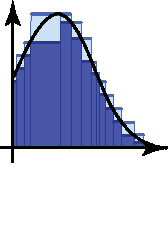
\includegraphics[trim=0cm 0cm 0cm 0cm, clip, scale=1.6]{images/lebesgueriemann1}
	\end{center}
\end{minipage}
\begin{minipage}{0.5\textwidth}
	\begin{center}
		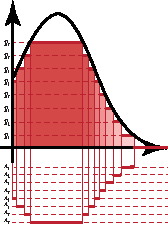
\includegraphics[trim=0cm 0cm 0cm 0cm, clip, scale=1.6]{images/lebesgueriemann2}
	\end{center}
\end{minipage}\\
In \textit{Sur le development de la notion d'intégrale (1926)} Lebesgue ripercorre il procedimento naturale alla base di questa idea fondamentale:
\blockquote{
	‘‘I geometri del diciassettesimo secolo considerano l'integrale di $f(x)$ - la parola \textit{integrale} non era ancora stata inventata, ma non importa - come la somma di un'infinità di indivisibili, ognuno dei quali era l'ordinata, positiva o negativa, di $f(x)$.\\
	Benissimo! Noi abbiamo semplicemente raggruppato insieme gli \textit{indivisibili} di 	grandezza vicina. Abbiamo, come si dice in algebra, riunito termini simili. Si potrebbe dire che, secondo il procedimento di Riemann, si cerca di sommare gli indivisibili prendendoli \textit{nell’ordine nel quale ci sono forniti dalla variazione di $x$}, come un commerciante confusionario che conta monete e biglietti a caso,	nell’ordine in cui gli vengono dati, mentre noi operiamo come un commerciante metodico che dice:
	\begin{center}
		 \begin{tabular}{l}
			«ho $m(G_1)$ monete da $100$, che valgono $100\ m(G_1)$»\\
			«ho $m(G_2)$ monete da $500$, che valgono $500\ m(G_2)$»\\
			«ho $m(G_3)$ biglietti da $1000$, che valgono $1000\ m(G_3)$»\\
			...
		\end{tabular}
	\end{center}
	Tutto insieme ho
	\begin{equation*}
		S=100\ m(G_1) + 500 m(G_2)+ 1000 m(G_3)+\ldots
	\end{equation*}
	I due procedimenti porteranno di certo il commerciante allo stesso risultato perché per quanti soldi abbia c’è solo un numero finito di monete e di biglietti da contare. Ma per noi che dobbiamo sommare un numero infinito di indivisibilità la differenza dei due metodi è \textit{di capitale importanza}.''
}
In altre parole, per calcolare l'integrale (secondo Lebesgue) di una funzione:
\begin{itemize}
	\item Suddividiamo l'immagine in intervalli e per ognuno di essi consideriamo un \textit{peso} dato dall'\textit{estremo inferiore} dei valori assunti dalla funzione nel dato intervallo.
	\item Consideriamo le controimmagini degli intervalli e associamo a ciascuna un valore detto \textbf{misura}.
	\item Calcoliamo un'approssimazione \textit{per difetto} dell'integrale sommando le misure che abbiamo ottenuto - ciascuna moltiplicata per il corrispondente peso.
	\item Più fitta è la partizione iniziale, più accurato sarà il valore dell'integrale.
\end{itemize}
\begin{intuit}
Poiché partizioniamo i \textit{valori} che assume una funzione e non il dominio in sè e li riordiniamo, possiamo trasformare delle funzioni particolarmente patologiche in funzioni ‘‘carine'' dal punto di vista dell'integrazione e ci consente di integrarle.
\end{intuit}
Osserviamo che l'idea di Lebesgue è decisamente geniale: non solo risolve i casi patologici che hanno afflitto i matematici del XIX secolo, ma ci permette di rivoluzionare completamente il concetto di integrale: dato che la partizione è effettuata sul \textit{codominio}, le funzioni non necessariamente devono essere definite sui reali, ma possiamo integrare funzioni definite su altri tipi di insiemi, come i naturali!\\
Tuttavia, abbiamo prima bisogno di affrontare alcune questioni:
\begin{enumerate}
	\item Dato che il dominio può essere un insieme qualsiasi, le controimmagini $f^{-1}\left(\left[y_i,y_{i+1}\right]\right)$ degli intervalli $\left[y_i,y_{i+1}\right]$ che otteniamo dalla partizione \textit{non} sono in generale intervalli: che cos'è la loro \textbf{misura}?
	\item Su quali insiemi è \textit{definibile} una misura?
	\item Per quali funzioni $f$ è possibile definire l'\textit{integrale}?
\end{enumerate}
Possiamo immaginare, da quanto detto, che una misura sia una funzione che quantifica la dimensione - che sia una lunghezza, un'area o volendo anche una cardinalità - di insiemi. Sostanzialmente, ci sono tre elementi da definire:
\begin{enumerate}[label=(\Roman*)]
	\item Una famiglia di insiemi su cui è definita una misura, che chiameremo poco intuitivamente $\sigma$\textbf{-algebra}, e i suoi elementi, che saranno detti \textbf{insiemi misurabili}.
	\item Una classe di funzioni su cui definire l’integrale, le \textbf{funzioni misurabili}.
	\item Ultima, ma decisamente non per importanza, una \textbf{misura} per valutare l’ampiezza degli insiemi.
\end{enumerate}
\section{Algebre e $\sigma$-algebre}
\begin{define}[Algebra]
	Sia $X$ un insieme qualsiasi. La famiglia $\mathcal{M}$ di sottoinsiemi di $X$ è una \textbf{algebra} \index{algebra} se soddisfa i seguenti assiomi:
	\begin{enumerate}
		\item L'\textit{insieme stesso} sta nell'algebra:
		\begin{equation}
			X\in\mathcal{M}
		\end{equation}
		\item L'algebra è chiusa rispetto alla \textit{complementarizzazione}: \begin{equation}
			A\in\mathcal{M}\implies A^C\in\mathcal{M}
		\end{equation}
		\item L'algebra è chiusa rispetto alla \textit{unione finita}:
		\begin{equation}
			A_1,\ \ldots,\ A_n\in\mathcal{M}\implies A_1\cup\ldots\cup A_n\in\mathcal{M}
		\end{equation}
	\end{enumerate}
\end{define}
Di queste nuove strutture matematiche ci interessano in particolare quelle che soddisfano un ulteriore condizione: la chiusura rispetto all'\textit{unione numerabile}.
\begin{define}[{$\sigma$}-algebra, spazi e insiemi misurabili]
	Sia $X$ un insieme qualsiasi. La famiglia $\mathcal{M}$ di sottoinsiemi di $X$ è una $\sigma$\textbf{-algebra} \index{{$\sigma$}-algebra} se soddisfa i seguenti assiomi:
	\begin{enumerate}
		\item L'\textit{insieme stesso} sta nell'algebra:
		\begin{equation}
			X\in\mathcal{M}
		\end{equation}
		\item L'algebra è chiusa rispetto alla \textit{complementarizzazione}: \begin{equation}
			A\in\mathcal{M}\implies A^C\in\mathcal{M}
		\end{equation}
		\item La $\sigma$-algebra è chiusa rispetto alla \textit{unione numerabile}: \begin{equation}
			A_n\in\mathcal{M}\implies \bigcup_{n\geq 1}A_n\in\mathcal{M} 
		\end{equation}
	\end{enumerate}
La coppia $\left(X,\mathcal{M}\right)$ si dice \textbf{spazio misurabile}\index{spazio!misurabile} e gli insiemi che appartengono a $\mathcal{M}$ sono detti \textbf{insiemi misurabili}\index{insieme!misurabile}.
\end{define}
\begin{observe}~{}
	\begin{itemize}
		\item $\emptyset\in\mathcal{M}$ in quanto è il complementare dell'insieme $X$.
		\item La $\sigma$-algebra è chiusa rispetto all'\textit{intersezione numerabile}:
		\begin{equation*}
			A_n\in\mathcal{M}\implies \bigcap_{n\geq 1}A_n\in\mathcal{M} 
		\end{equation*}
		Infatti, l'intersezione si può scrivere tramite unioni e complementari, operazioni interne alla $\sigma$-algebra, grazie alle \textit{leggi di De Morgan}\footnote{Nelle ‘‘Note aggiuntive'', a pagina \pageref{leggidemorgan} è possibile trovare alcune informazioni sulle leggi di De Morgan.}.
	\end{itemize}
\end{observe}
\begin{example}
	Ogni insieme si può dotare della struttura di spazio misurabile, in quanto ammette almeno la $\sigma$-algebra triviale data da $\setpart{X}$.
\end{example}
\begin{define}[{$\sigma$}-algebra generata da una famiglia di sottoinsiemi]
	Data una famiglia $\mathcal{F}$ di sottoinsiemi di $X$, si dice $\sigma$-\textbf{algebra generata da} $\mathcal{F}$\index{{$\sigma$}-algebra!generata da una famiglia di sottoinsiemi} l'intersezione di \textit{tutte} le $\sigma$-algebre che contengono $\mathcal{F}$ ed è la più piccola $\sigma$-algebra che contiene $\mathcal{F}$.
\end{define}
\begin{example}
	Se $X$ è spazio \textit{topologico} e $\mathcal{F}$ è la famiglia degli \textit{aperti} di $X$ (che coincide con la \textit{topologia} $\tau$ se definita con gli assiomi degli aperti), la $\sigma$-algebra generata da $\mathcal{F}$ si chiama $\sigma$\textbf{-algebra dei Boreliani di} $X$\index{{$\sigma$}-algebra!dei Boreliani} e si indica con $\mathcal{B}(x)$.\\
	Osserviamo che la famiglia $\mathcal{F}$ di per sé non è una $\sigma$-algebra: se $A$ è aperto, $A^C$ è chiuso e quindi non appartiene a $\mathcal{F}$; invece, in $\mathcal{B}(x)$ ci stanno anche i chiusi della topologia e quindi la complementarizzazione è un'operazione interna.
\end{example}
\section{Funzioni misurabili}
\begin{define}[Funzione misurabile]
	Sia $\left(X, \mathcal{M}\right)$ spazio misurabile e $Y$ spazio topologico. Una funzione $\funz{f}{X}{Y}$ si dice \textbf{misurabile}\index{funzione!misurabile} se \begin{equation}
		f^{-1}\left(A\right)\in\mathcal{M},\ \forall A\subseteq Y\text{ aperto.}
	\end{equation}
\end{define}
\begin{observe}
	Se $\mathcal{M}=\setpart{X}$, allora \textit{ogni} funzione è misurabile.
\end{observe}
\begin{examples}~{}
	\begin{enumerate}
		\item Sia $\left(X,\mathcal{B}(x)\right)$ spazio misurabile su $X$ spazio topologico con la $\sigma$-algebra dei Boreliani di $X$ e sia $Y$ spazio topologico. Allora
		\begin{center}
			$\funz{f}{X}{Y}$ continua$\implies \funz{f}{X}{Y}$ misurabile.
		\end{center}
	Infatti, $\forall A\subseteq Y$ aperto, $f^{-1}\left(A\right)$ è aperto per continuità di $f$ e quindi $f^{-1}\left(A\right)\in\mathcal{B}(x)$.
	\item Sia $\left(X,\mathcal{M}\right)$ spazio misurabile qualsiasi e sia $E\subseteq X$. Definiamo la \textbf{funzione caratteristica di} $E$\index{funzione!caratteristica di un sottoinsieme} o \textbf{indicatrice di} $E$\seeonlyindex{funzione!caratteristica di un sottoinsieme}{indicatrice di un sottoinsieme} la funzione
	\begin{equation}
		\funztot{\chi_E}{X}{\realset}{x}{\chi_E(x)=\begin{cases}
				\begin{array}{ll}
					1&\text{se }x\in E\\
					0&\text{se }x\notin E\\
				\end{array}
		\end{cases}}
	\end{equation}
Allora
\begin{center}
$\chi_E$ è misurabile $\iff E\in\mathcal{M}$
\end{center}
Infatti, preso $A\subseteq \realset$, si ha
\begin{equation*}
f^{-1}\left(A\right)=\begin{cases}
	\begin{array}{ll}
		\emptyset&\text{se }0\notin A,\ 1\notin A\\
		E^C&\text{se }0\in A,\ 1\notin A\\
		E&\text{se }0\notin A,\ 1\in A\\
		X&\text{se }0\in A,\ 1\in A
	\end{array}
\end{cases}
\end{equation*}
Allora $f^{-1}\left(A\right)\in\mathcal{M}\iff E\in\mathcal{M}$.
\end{enumerate}
\end{examples}
\begin{observe}
	La funzione caratteristica $\chi_{\rationalset\cap\left[0,1\right]}$ è la \textbf{funzione di Dirichlet}\footnote{Si veda pag. \pageref{funzionedirichlet}.}.
\end{observe}
\begin{propertiesqed}[Proprietà della funzioni misurabili]\label{funzionimisurabilicomplesse}~
	\begin{enumerate}
		\item Sia $\left(X,\mathcal{M}\right)$ uno spazio misurabile e sia $\funz{f}{X}{\complexset}$, dove $\complexset$ ha la topologia Euclidea. Possiamo ‘‘scomporre'' la funzione a valori complessi come combinazione lineare di funzioni reali rispetto alla base $(1,i)$.
		\begin{center}
			$\forall x\in X f(x)\in\complexset\implies f(x)=\underbrace{u(x)}_{\text{parte reale}}+i\underbrace{v(x)}_{\text{parte imm.}}$, con $\funz{u,v}{X}{\realset}$.
		\end{center}
	Allora
	\begin{enumerate}
		\item $f$ è misurabile$\implies u,\ v,\ \abs{f}$ misurabili.
		\item $u, v$ sono misurabili$\implies f=u+iv$ è misurabile.
	\end{enumerate}
\item Siano $\funz{f,g}{X}{\complexset}$. Se $f,g$ sono misurabili, allora
\begin{itemize}
	\item $f+g$ è misurabile.
	\item $fg$ è misurabile.\qedhere
\end{itemize}
\end{enumerate}
\end{propertiesqed}
\subsection{Caratterizzazione delle funzioni misurabili}
In \textsc{Calcolo delle Probabilità} abbiamo dato una definizione di funzione misurabile $\funz{f}{\left(X,\mathcal{M}\right)}{Y}$ se la controimmagine tramite $f$ di un Boreliano è un insieme misurabile per $\mathcal{M}$. Vedremo ora come questa definizione è equivalente a quella data all'inizio della sezione.
\begin{theoremasqed}[Caratterizzazione delle funzioni misurabili]~
	\begin{enumerate}\label{caratterizzazionefunzionimisurabili}
		\item La funzione $\funz{f}{\left(X,\mathcal{M}\right)}{Y}$, con $Y$ spazio topologico, è  misurabile se e solo se
		\begin{equation}
			f^{-1}\left(B\right)\in\mathcal{M},\ \forall B \text{ Boreliano di } Y.
		\end{equation}
		\item Posto $Y=\realset^{\ast}=\left[-\infty,+\infty\right]$, $\funz{f}{X}{\left[-\infty,+\infty\right]}$ è misurabile se e solo se
		\begin{equation}
			f\left(\left(\alpha,+\infty\right]\right)\in\mathcal{M},\ \forall \alpha\in\realset.\qedhere
		\end{equation}
	\end{enumerate}
\end{theoremasqed}
Che differenza c'è tra la definizione e le caratterizzazioni? In sostanza possono essere considerate tre ‘‘test'' differenti per mostrare o confutare che una funzione sia misurabile.
\begin{align*}
	\circled[red]{A}&\qquad f^{-1}\left(A\right)\in\mathcal{M},\ \forall A\text{ aperto di }Y\\
	\circled[red]{B}&\qquad f^{-1}\left(B\right)\in\mathcal{M},\ \forall B\text{ Boreliano di }Y\\
	\circled[red]{C}&\qquad f^{-1}\left(\left(\alpha,+\infty\right]\right)\in\mathcal{M},\ \forall \alpha\in\realset,\ \text{con }Y=\realset^{\ast}=\left[-\infty,+\infty\right]
\end{align*}
Da un punto di vista \textit{operativo} \circled[red]{B} non conviene come metodo per verificare che $f$ sia misurabile: i Boreliani, pur avendo la \textit{stessa cardinalità} degli aperti, li contengono \textit{strettamente}\footnote{A pag. \pageref{famigliediinsiemi} è possibile trovare un approfondimento sulla relazione tra Boreliani, aperti e altre classi di insiemi.} e quindi bisogna verificare ulteriori insiemi (come i chiusi) rispetto a quelli che si verificherebbero con la condizione \circled[red]{A}.\\
Tuttavia, \circled[red]{B} fornisce delle informazioni che immediatamente non si avevano dalla definizione originale: sono misurabili non solo le controimmagini degli aperti, ma anche le controimmagini dei chiusi.\\
Col caso \circled[red]{C} ci limitiamo ad operare in $\realset^{\ast}=\left[-\infty,+\infty\right]$, ma è sicuramente più vantaggioso da applicare rispetto ad \circled[red]{A}.
\subsection{Passaggio al limite per funzioni misurabili}
Ci chiediamo se, date $f_n$ successione di funzioni misurabili che convengono ad una funzione $f$ in \textit{una qualche} convergenza, $f$ risulta essere ancora misurabile e se sì, con quale tipo di convergenza.\\
A differenza di quanto visto col passaggio al limite della continuità, la risposta è affermativa anche sotto la sola ipotesi di \textit{convergenza puntuale}!\\
Per dimostrarlo (e lo faremo per funzioni a valori in $\complexset$), abbiamo bisogno di alcuni risultati preliminari che riguardano $\sup$, $\inf$, $\limsup$, $\liminf$ di una successione di funzione. Per poter parlare di $\limsup$ e $\liminf$ abbiamo bisogno di avere il codomini della funzione in uno spazio $Y$ con ordinamento, pertanto ci porremo in  $\realset^{\ast}=\left[-\infty,+\infty\right]$, ossia le nostre funzioni saranno del tipo
\begin{equation*}
\funz{f}{\left(X,\mathcal{M}\right)}{\realset^{\ast}=\left[-\infty,+\infty\right]}
\end{equation*}
\begin{define}[{$\sup$}, {$\inf$}, {$\limsup$} e {$\liminf$} di una successione di funzioni]
Sia $\funz{f_n}{\left(X,\mathcal{M}\right)}{\realset^{\ast}=\left[-\infty,+\infty\right]}$ misurabili.
Allora definiamo:
\begin{gather*}
	\left(\sup_{n\geq 1} f_n\right)(x)\coloneqq \sup_{n\geq 1}f_n(x),\ \forall x\in X\\
	\left(\inf_{n\geq 1} f_n\right)(x)\coloneqq \inf_{n\geq 1}f_n(x),\ \forall x\in X\\
	\left(\limsup_{n\to+\infty} f_n\right)(x)\coloneqq \limsup_{n\to+\infty}f_n(x),\ \forall x\in X\\
	\left(\liminf_{n\to+\infty} f_n\right)(x)\coloneqq \liminf_{n\to+\infty}f_n(x),\ \forall x\in X
\end{gather*}
\end{define}
\begin{proposition}[Misurabilità di {$\sup$}, {$\inf$}, {$\limsup$} e {$\liminf$} di una successione di funzioni misurabili]\label{misurabilitàsupinf}
	Sia $ \left(X,\mathcal{M}\right)$ uno spazio misurabile e siano $\funz{f_n}{\left(X,\mathcal{M}\right)}{\realset^{\ast}=\left[-\infty,+\infty\right]}$ misurabili.
	Allora
	\begin{equation*}
		\sup_{n\geq 1} f_n\quad\inf_{n\geq 1} f_n\quad\limsup_{n\to\infty} f_n\quad\liminf_{n\to\infty} f_n
	\end{equation*}
sono misurabili.
\end{proposition}
\begin{demonstration}~{}
	\begin{enumerate}
		\item Sia $\displaystyle g(x)=\sup_{n\geq 1} f_n(x),\ \forall x\in X$. Dobbiamo provare che $g$ sia misurabile, con $\funz{g}{\left(X,\mathcal{M}\right)}{\realset^{\ast}=\left[-\infty,+\infty\right]}$. Per il teorema \ref{caratterizzazionefunzionimisurabili} sulla \textit{caratterizzazione} delle funzioni misurabili è sufficiente dimostrare che $g^{-1}\left(\left(\alpha,+\infty\right]\right)\in\mathcal{M},\ \forall\alpha\in\realset$.\\
		Innanzitutto, mostriamo che
		\begin{equation*}
			g^{-1}\left(\left(\alpha,+\infty\right]\right)=\bigcup_{n\geq 1}f_n^{-1}\left(\left(\alpha,+\infty\right]\right),\ \forall \alpha\in\realset.
		\end{equation*}
	Infatti:
	\begin{align*}
		x\in g^{-1}\left(\left(\alpha,+\infty\right]\right)&\iff g(x)>\alpha\\
		& \iff \exists j\geq 1\colon f_j(x)>\alpha\\
		& \iff \exists j\geq x\in f_j^{-1}\left(\left(\alpha,+\infty\right]\right)\\
		& \iff x\in \bigcup_{n\geq 1}f_n^{-1}\left(\left(\alpha,+\infty\right]\right).
	\end{align*}
	Poiché $f_n$ è misurabile si ha
	\begin{equation*}
		f_n^{-1}\left(\left(\alpha,+\infty\right]\right)\in\mathcal{M}
	\end{equation*}
ed essendo $\mathcal{M}$ una $\sigma$-algebra è chiusa rispetto all'unione misurabile e dunque
	\begin{equation*}
	g^{-1}\left(\left(\alpha,+\infty\right]\right)=\bigcup_{n\geq 1}f_n^{-1}\left(\left(\alpha,+\infty\right]\right)\in\mathcal{M}
	\end{equation*}
	\item[2,3,4.] Si riconducono al caso $1)$ perché
	\begin{gather*}
		\inf_{n\geq 1}f_n=-\left(\sup_{n\geq 1}\left(-f_n\right)\right)\\
		\limsup_{n\to+\infty}f_n=\inf_{k\geq 1}\sup_{n\geq k}f_n\\
		\liminf_{n\to+\infty}f_n=\sup_{k\geq 1}\inf_{n\geq k}f_n\qedhere
	\end{gather*}
	\end{enumerate}
\end{demonstration}
\begin{corollary}[Passaggio al limite per funzioni misurabili in {$\complexset$}]
	Sia $\left(X,\mathcal{M}\right)$ uno spazio misurabile e siano $\funz{f_n}{X}{\complexset}$.\\
	Se $f_n$ sono misurabili ed esiste $\funz{f}{X}{\complexset}$ tale che
	\begin{equation*}
		\lim_{n\to+\infty}f_n(x)=f(x),\ \forall x\in X
	\end{equation*}
	allora $f$ è misurabile.
\end{corollary}
\begin{demonstration}
	Riconduciamoci al caso reale per utilizzare la proposizione precedente. Posto
	\begin{equation*}
		f_n=u_n+iv_n\qquad f=u+iv
	\end{equation*}
dove
\begin{equation*}
	\begin{array}{ll}
		\funz{u_n=\Re\left(f_n\right)}{X}{\realset}&\funz{v_n=\Im\left(f_n\right)}{X}{\realset}\\
		\funz{u=\Re\left(f\right)}{X}{\realset}&\funz{v=\Im\left(f\right)}{X}{\realset}
	\end{array}
\end{equation*}
Come visto nella proposizione \ref{funzionimisurabilicomplesse}, $f_n$ misurabile implica che sia $u_n$ sia $v_n$ siano misurabili e, dal risultato precedente sulle funzioni a valori in $\realset^{\ast}$ si ha
\begin{equation*}
	\limsup_{n\to+\infty}u_n,\ \limsup_{n\to+\infty}v_n\text{ misurabili.}
\end{equation*}
D'altra parte si ha
\begin{equation*}
	\lim_{n\to+\infty}f_n(x)=f(x)\implies
	\begin{cases}
		\displaystyle\lim_{n\to+\infty}u_n(x)=u(x)\\
		\displaystyle\lim_{n\to+\infty}v_n(x)=v(x)
	\end{cases}
\end{equation*}
Poiché i limiti esistono si ha
\begin{gather*}
	\lim_{n\to+\infty}u_n=\limsup_{n\to+\infty}u_n=u(x)\\	\lim_{n\to+\infty}v_n=\limsup_{n\to+\infty}v_n=v(x)
\end{gather*}
Quindi $u(x)$ e $v(x)$ sono misurabili, pertanto anche $f=u+iv$ è misurabile.
\end{demonstration}
\section{Misura di Peano-Jordan}
Negli stessi anni in cui si lavorò per espandere la classe di funzioni che ammettono integrale definito, diversi matematici lavorano su un'altra questione, quella della \textbf{misura} di un insieme.\\
Chiaramente già dall'antichità erano note misure di figure ‘‘elementari'', come ad esempio la lunghezza e l'area di un poligono o il volume di certi solidi, spesso sulla base di principi come quello di \textit{esaustione}.\\
Solo nel XIX secolo si cercò di formalizzare questi ragionamenti ed espandere il concetto di misura non soltanto a figure generiche, ma anche a più dimensioni fino ad arrivare ad una astrazione di tale concetto ad insiemi, indipendentemente dall'essere in $\realset^n$.\\
Il primo ad introdurre un concetto di misura di un sottoinsieme della retta, del piano o delle spazio fu Giuseppe \textbf{Peano} (1858-1932). Nel suo \textit{Applicazioni geometriche del
calcolo infinitesimale (1887)}, il matematico torinese ipotizza di ‘‘modernizzare'' il metodo di esaustione già citato in precedenza.
Ad esempio, prendo un insieme limitato in $\realset^2$, ossia quello che all'epoca veniva denominato \textit{campo piano}, potremmo considerare dei poligoni che contengono tale insieme - che chiameremo \textit{poligoni esterni} - e dei poligoni che sono contenuti in tale insieme - i cosiddetti \textit{poligoni interni}.
\begin{center}
	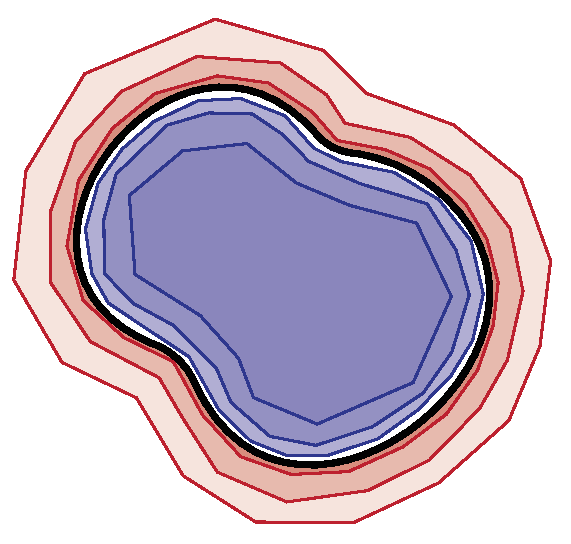
\includegraphics[trim=0cm 0cm 0cm 0cm, clip, scale=0.71]{images/peanopoligoni.pdf}
\end{center}
Se l'estremo inferiore dei poligoni esterni coincide con quello superiore di quelli interni, potremmo dire che l'insieme è misurabile e ha area pari a questo limite.
Inoltre, Peano fornisce una condizione necessaria e sufficiente: la differenza tra i poligoni esterni ed interni deve essere piccola a piacere, ossia la frontiera dell'insieme (che chiaramente è contenuta nell'area di piano fra i poligoni esterni ed interni) dovrà avere misura nulla.\\
Possono capitare anche insiemi che non ammettono area. 
\begin{example}
	Supponiamo di prendere tutti i punti a distanza \textit{razionale} $r\leq 1$ dall'origine, cioè infinite circonferenze di raggio razionale interne al disco di raggio 1.\\
	Chiaramente l'area interna è uguale a 0, mentre essendo l'insieme denso nel disco di raggio 1, ogni poligono che la contiene contiene il cerchio e quindi l'area esterna è maggiore o uguale 1: essendo l'area interna e l'area esterna diverse, il poligono non ammette aree.
\end{example}
La misura di Peano, per quanto innovativa, risente di alcuni problemi: parlare di poligoni o solidi poligonali è facile farlo in $\realset^2$ o $\realset^3$, ma non è generalizzabile in dimensioni maggiori: ad esempio, qual è la misura di un ipersolido poligonale di dimensione 4? Inoltre, la misura di Peano non è numerabilmente additiva, ossia un'unione \textit{infinita numerabile} di insiemi misurabili secondo Peano non è necessariamente ancora misurabile.\\
Qualche anno dopo i lavori di Peano, il matematico francese Marie Camille \textbf{Jordan} (1838-1922) \textit{estende} il concetto di misura introdotta da Peano a una generica dimensione $n$, utilizzando invece che poligoni o solidi poligoni delle \textit{unioni di intervalli}, \textit{rettangoli} o, in generale, \textit{parallelepipedi} $n$-dimensionali, poiché questi hanno una misura ben nota!
\begin{center}
	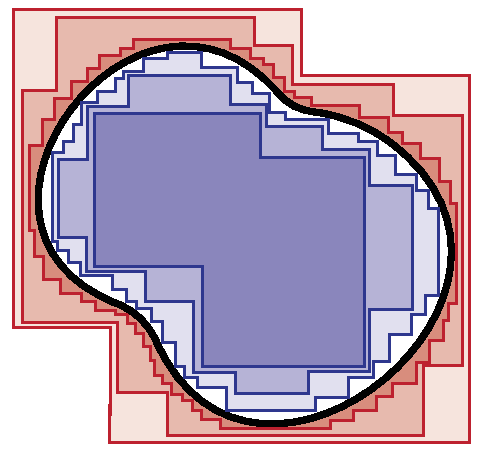
\includegraphics[trim=0cm 0cm 0cm 0cm, clip, scale=0.71]{images/peanoparallelepipedi.pdf}
\end{center}
Anche se questa misura coincide con quella di Peano (dopotutto, le unioni di parallelepipedi sono un \textit{caso particolare} di ipersolidi poligonali), in questo modo si risolve il \textit{primo problema} dei due problemi enunciati precedentemente; ciò nonostante, questa definizione non è ancora una misura numerabilmente-additiva.
\subsection{Definizione e osservazioni sulla misura di Peano-Jordan}
\begin{define}[Parallelepipedo {$n$}-dimensionale]
	Un \textbf{parallelepipedo}\index{parallelepipedo} $n$-dimensionale è un \textit{plurintervallo}, ossia un prodotto cartesiano di $n$ intervalli:
	\begin{equation}
		P=\prod_{i=1}^{n}\left[a_i,b_i\right]\quad\text{con }-\infty < a_i < b_i < +\infty
	\end{equation}
	Posta la \textbf{lunghezza}\index{lunghezza!di un intervallo} di un intervallo come
		\begin{equation}
			\mathcal{L}\left(\left[a_i,b_i\right]\right)=b_i-a_i
		\end{equation}
		la misura $n$-dimensionale del parallelepipedo è
		\begin{equation}
			V_n(P)=\prod_{i=1}^{n}\mathcal{L}\left(\left[a_i,b_i\right]\right)
		\end{equation}
	\end{define}
	Introduciamo formalmente la misura esterna e la misura interna di un insieme limitato $A$ come estremi inferiori e superiori di un \textbf{insieme elementare}\index{insieme!elementare}, cioè un'unione finita di parallelepipedi:
	\begin{itemize}
		\item \textsc{Misura esterna}:\index{misura!esterna} \begin{equation}
			m_{PJ}^X\left(A\right)=\inf\left\{\sum_{i=1}^{n}V_n\left(P_i\right)\mid P_i\text{ parallelepipedi},\ \bigcup_{i=1}^nP_i\supseteq A\right\}
		\end{equation}
		\item \textsc{Misura interna}:\index{misura!interna}
		\begin{equation}
			m_{PJ,X}\left(A\right)=\inf\left\{\sum_{i=1}^{n}V_n\left(P_i\right)\mid P_i\text{ parallelepipedi},\ \bigcup_{i=1}^nP_i\subseteq A\right\}
		\end{equation}
	\end{itemize}
	In generale $m_{PJ,X}\left(A\right)\leq m_{PJ}^{X}\left(A\right)$.
	\begin{define}[Misura di Peano-Jordan]
		Un insieme limitato $A$ è \textbf{misurabile secondo Peano-Jordan}\index{misura!secondo Peano-Jordan} se
		\begin{equation}
			m_{PJ}^X\left(A\right)=m_{PJ,X}\left(A\right)
		\end{equation}
	e la \textbf{misura} (secondo P-J) dell'insieme è
		\begin{equation}
			m_{PJ}\left(A\right)=m_{PJ}^X\left(A\right)=m_{PJ,X}\left(A\right)
		\end{equation}
	\end{define}
	\begin{propositionqed}[Criterio di misurabilità]
		L'insieme limitato $A\subseteq \realset^n$ è misurabile per Peano-Jordan se e solo se $\forall \epsilon>0,\ \exists P\subseteq A, Q\supseteq A$ con $P,\ Q$ insiemi elementari tali che
		\begin{equation}
			m_{PJ}\left(Q\right)-m_{PJ}(P)\leq \epsilon\qedhere
		\end{equation}
	\end{propositionqed}
	Definito
	\begin{equation}
		\mathcal{M}=\left\{A\subseteq \realset^n\mid A\text{è P-J misurabile}\right\}
	\end{equation}
	essa è un'\textit{algebra}, \textit{ma} non una $\sigma$-algebra, cioè non è chiusa rispetto all'unione \textit{numerabile infinita}.
	\begin{examplewt}[Controesempio dell'additività numerabile della misura di P-J]
		Consideriamo
		\begin{equation*}
			E=\rationalset\cap\left[0,1\right]=\bigcup_{n\geq 1}\left\{r_n\right\}
		\end{equation*}
		dove $\left\{r_n\right\}$ è un'enumerazione di razionali in $\left[0,1\right]$.\\
		$\left\{r_n\right\}$ è un punto e dunque è misurabile con misura nulla, ma \begin{equation*}
			\bigcup_{n\geq 1}\left\{r_n\right\}=E
		\end{equation*}
		\textit{non} è misurabile, dato che
		\begin{equation*}
			\begin{cases}
				m_{PJ}^X(E)=1\\
				m_{PJ,X}(E)=0
			\end{cases}
		\end{equation*}
	\end{examplewt}
	In altre parole, la misura secondo Peano-Jordan è \textit{additiva}, ma non $\sigma$-additiva.
	\begin{digression}
		Nella letteratura italiana si è soliti parlare ‘‘misura di Peano-Jordan'', quando in realtà questa terminologia è impropria, non essendo una \textit{misura} nel senso \textit{moderno} del termine. Nell'anglosfera lo stesso concetto viene chiamato ‘‘Jordan content'.
	\end{digression}
	\section{Misura secondo Lebesgue}
	Per quanto innovativa, la misura di Peano-Jordan presenta alcuni notevoli problemi:
	\begin{itemize}
		\item É definita solo per \textit{insiemi limitati}.
		\item Non è \textit{numerabilmente additività}: la misura di un'unione numerabilmente infinita di insiemi misurabili non è necessariamente misurabile.
	\end{itemize}
	Il concetto \textit{moderno} di misura di un sottoinsieme dello spazio $n$-dimensionale viene per la prima volta presentato in \textit{Intégrale, longueure, aire} (1902)
	dal matematico francese Henri \textbf{Lebesgue} (1875-1941) nell'ambito dell'annoso problema delle discontinuità nell'integrale definito.\\
	La costruzione della misura secondo Lebesgue inizia in modo analogo a quella di Peano-Jordan, definendo i \textit{parallelepipedi}; per poter definire la misurabilità di insiemi illimitati si ammettono parallelepipedi \textit{degeneri}.
	\begin{define}[Parallelepipedo {$n$}-dimensionale]
		Un \textbf{parallelepipedo}\index{parallelepipedo} $n$-dimensionale è un \textit{plurintervallo}, ossia un prodotto cartesiano di $n$ intervalli eventualmente \textit{degeneri}:
		\begin{equation}
			P=\prod_{i=1}^{n}\left[a_i,b_i\right]\quad\text{con }-\infty \leq a_i \leq b_i \leq +\infty
		\end{equation}
		Posta la \textbf{lunghezza}\index{lunghezza!di un intervallo} di un intervallo come
		\begin{equation}
			\mathcal{L}\left(\left[a_i,b_i\right]\right)=
			\begin{cases}
				\begin{array}{ll}
					b_i-a_i & \text{se }-\infty < a_i \leq b_i < +\infty\\
					+\infty&\text{altrimenti}
				\end{array}
			\end{cases}
		\end{equation}
		la misura $n$-dimensionale del parallelepipedo è
		\begin{equation}
			V_n(P)=\prod_{i=1}^{n}\mathcal{L}\left(\left[a_i,b_i\right]\right)
		\end{equation}
		con la convenzione che $0\cdot \infty =0$.
	\end{define}
	\begin{observe}
		Come mai $0\cdot \infty$ non è lasciato indeterminato, ma posto proprio uguale a 0?. Per capirlo, facciamo prima un esempio in dimensione 2; consideriamo il rettangolo degenere
		\begin{equation*}
			P=\left\{a_1\right\}\times\left(a_2,+\infty\right).
		\end{equation*}
		Esso è un sottoinsieme di $\realset^2$, ma ha chiaramente una sola dimensione: seppur come semiretta ha una lunghezza ben definita (e in tal caso sarebbe infinita tale lunghezza), è ragionevole dire che come oggetto \textit{bidimensionale} abbia \textit{area} $0$.
		\begin{center}
			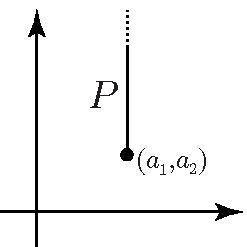
\includegraphics[trim=0cm 0cm 0cm 0cm, clip, scale=0.71]{images/rettangolodegenere.pdf}
		\end{center}
		In altre parole, se almeno un intervallo che compone il parallelepipedo $n$-dimensionale ha lunghezza nulla, $P$ è da intendersi come elemento di dimensione $k$ in uno spazio $n$-dimensionale, con $k< n$.
		In questo caso, la sua misura $n$\textit{-dimensionale} è nulla, anche se fosse \textit{illimitato} in diverse direzioni, da qui spiegato il perché di $0\cdot \infty =0$.
	\end{observe}
	A differenza di Peano-Jordan, Lebesgue definisce solamente la \textbf{misura esterna} dell'insieme:
	\begin{equation}
		m^X\left(A\right)=\inf\left\{\sum_{i=1}^{n}V_n\left(P_i\right)\middle| P_i\text{ parallelepipedi aperti},\ \bigcup_{i=1}^nP_i\supseteq A\right\}
	\end{equation}
dove per parallelepipedo \textit{aperti} si intende un plurintervallo definito da intervalli aperti.\\ 
	Essa si può vedere come una funzione
	\begin{equation}
		\funz{m^X}{\setpart{\realset^n}}{\left[0,+\infty\right]}
	\end{equation}
	che gode delle seguenti proprietà:
	\begin{itemize}
		\item Se l'insieme è un parallelepipedo $n$-dimensionale, la misura esterna del parallelepipedo ovviamente coincide con la misura $n$-dimensionale di esso:
		\begin{equation}
			m^X(P)=V_n(P),\ \forall P\text{ parallelepipedo}
		\end{equation}
		\item È \textit{monotona}:
		\begin{equation}
			m^X\left(A\right)\leq m^X\left(B\right),\ \forall A\subseteq B
		\end{equation}
		\item È $\sigma$-\textit{subadditiva}:
		\begin{equation}
			m^X\left(\bigcup_{n\geq 1}A_n\right)\leq \sum_{n\geq 1}m^X\left(A_n\right), \forall A_n\subseteq \realset^n
		\end{equation}
		\item È \textit{invariante per traslazioni}:
		\begin{equation}
			m^X\left(A+\left\{x\right\}\right)=m^X\left(A\right),\ \forall x\in\realset^n,\ \forall A\subseteq\realset^n
		\end{equation}
	\end{itemize}
	Osserviamo che per $m^X$ vale \textit{solo} la  $\sigma$-\textit{subadditività}, ma non la $\sigma$-\textit{additività}.
	\begin{define}[Insieme misurabile secondo Lebesgue {{\small (Criterio di Caratheodory)}}]\index{criterio!di Caratheodory}
		Un insieme $A\subseteq\realset^n$ è \textbf{misurabile secondo Lebesgue} se $\forall E\subseteq\realset^n$ vale
		\begin{equation}
			m_n^X(E)=m_n^X\left(E\cap A\right)+m_n^X\left(E\cap A^C\right)
		\end{equation}
	\end{define}
	$E$ è un \textbf{insieme test}\index{insieme!test} arbitrario (non necessariamente misurabile!): $A$ è misurabile se decompone bene $E$ in due sottoinsiemi misurabili $E\cap A$ e $E\cap A^C$.
	\begin{center}
		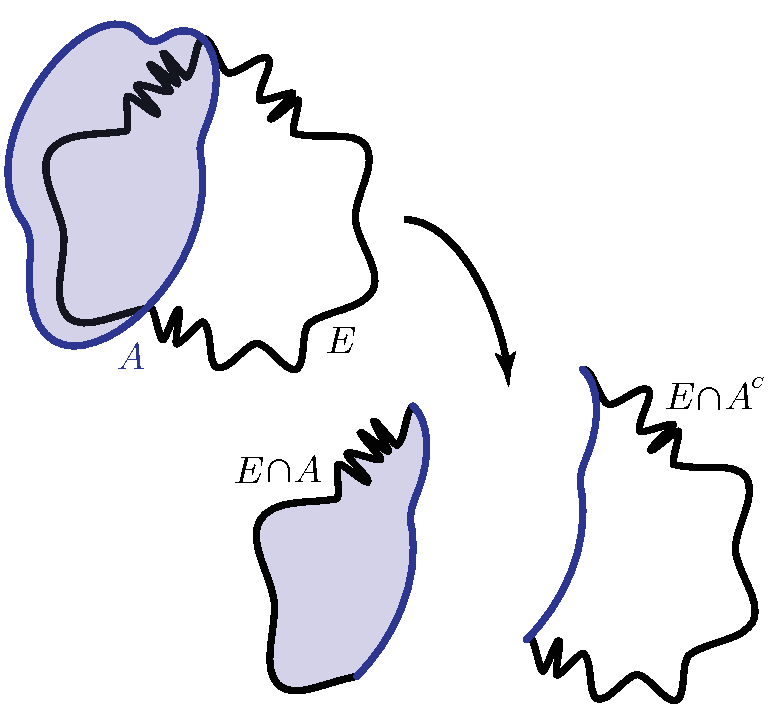
\includegraphics[trim=0cm 0cm 0cm 0cm, clip, scale=0.5]{images/criteriomisurabilita.pdf}
	\end{center}
	\begin{propositionqed}[Gli insiemi misurabili secondo Lebesgue sono una {$\sigma$}-algebra]
		La collezione di insiemi
		\begin{equation*}
			\mathcal{L}\left(\realset^n\right)=\left\{A\subseteq \realset^n\mid A\text{ è Lebesgue-misurabile}\right\}
		\end{equation*}
		è una $\sigma$-algebra.
	\end{propositionqed}
	\begin{define}[Misura secondo Lebesgue]
		La \textbf{misura secondo Lebesgue}\index{misura!secondo Lebesgue} è la restrizione della misura esterna a $\mathcal{L}\left(\realset^n\right)$:
		\begin{equation}
			m_n={m^X_n}\vert_{ \mathcal{L}\left(\realset^n\right)}\text{ ossia }\funz{m_n}{\mathcal{L}\left(\realset^n\right)}{\left[0,+\infty\right]}
		\end{equation}
	\end{define}
\subsection{Insiemi misurabili secondo Lebesgue}
La definizione data di insieme misurabile secondo Lebesgue non è particolarmente \textit{operativa}, in quanto richiede di controllare che un generico insieme test decomponga bene l'insieme di cui vogliamo verificare la misurabilità.
Di seguito presentiamo alcune classi importanti di insiemi misurabili secondo Lebesgue.
\begin{itemize}
	\item \textsc{\textbf{Insiemi elementari:}} (unioni di) parallelepipedi, anche degeneri:
	\begin{gather*}
		m_n(P)=V_n(P)\\
		m_n\left(\bigcup_{i=1}^{+\infty} P_i\right)=\sum_{i=1}^{+\infty}V_n\left(P_i\right)
	\end{gather*}
In particolare:
\begin{itemize}
	\item Preso $P=\realset^n$, allora $m_n\left(\realset^n\right)=+\infty$.
	\item Preso $P=\left\{x\right\},\ \forall x\in\realset^n$, allora $m_n\left(\left\{x\right\}\right)=0$.
\end{itemize}
\item \textsc{\textbf{Boreliani:}} $\mathcal{B}\left(\realset^n\right)\subsetneqq\mathcal{L}\left(\realset^n\right)$.\\
È importante sottolineare che ci sono insiemi misurabili \textit{non} Boreliani.\footnote{Si veda pag. \pageref{funzionecantor}.}
\item \textsc{\textbf{Tutti gli insiemi aventi misura \textit{esterna} nulla:}}
\begin{equation*}
	\forall A\subseteq \realset^n\ m_n^X\left(A\right)=0\implies A\in\mathcal{L}\left(\realset^n\right)\text{ e }m_n\left(A\right)=0
\end{equation*}
\end{itemize}

\begin{demonstration}
	Dobbiamo provare che $\forall E\subseteq \realset^n$
	\begin{equation*}
		m_n^X(E)=m_n^X\left(E\cap A\right)+m_n^X\left(E\cap A^C\right)
	\end{equation*}
	Ricordiamo che $m_n^X$ è $\sigma$-subadditiva e quindi finito-subadditiva, quindi
	\begin{equation*}
		E=\left(E\cap A\right)\cup \left(E\cap A^C\right)\implies m_n^X(E)\leq m_n^X\left(E\cap A\right)+m_n^X\left(E\cap A^C\right)
	\end{equation*}
	È sufficiente allora provare la disuguaglianza opposta. Osserviamo che $E\cap A^C\subseteq E$, dunque per monotonia di $m_n^X$ si ha
	\begin{equation*}
		m_n^X(E)\geq m_n^X\left(E\cap A^C\right)=m_n^X\left(E\cap A^C\right)+0=m_n^X\left(E\cap A^C\right)+m_n^X\left(E\cap A\right)
	\end{equation*}
	Infatti $E\cap A\subseteq A$ implica, per monotonia di $m_n^X$ che
	\begin{equation*}
		0\leq m_n^X\left(E\cap A\right)\leq m_n^X\left(A\right)=0
	\end{equation*}
	e quindi $m_n^X(E)\geq m_n^X\left(E\cap A^C\right)+m_n^X\left(E\cap A\right)$.
\end{demonstration}
\begin{attention}
	\textbf{Non} tutti gli insiemi sono misurabili! Se supponiamo vero l'Assioma della Scelta, l'\textbf{insieme di Vitali} è un insieme non misurabile in $\realset$ rispetto alla misura di Lebesgue unidimensionale\footnote{Si veda pag. \pageref{vitali} per la definizione dell'insieme di Vitali e la dimostrazione di ciò.}.
\end{attention}
Nella teoria di Lebesgue hanno un ruolo importante gli insiemi di misura nulla: esplicitiamo il legame tra misura nulla e cardinalità.
È noto che ogni singolo punto ha misura nulla; osserviamo che presa una famiglia di punti $\left\{x_n\right\}$ si ha
\begin{equation*}
	0\leq m_n\left(\bigcup_{n\geq 1}\left\{x_n\right\}\right)\leq \sum_{n\geq 1}m_n\left(\left\{x_n\right\}\right)=0
\end{equation*}
Ogni insieme \textbf{numerabile} è misurabile e ha misura nulla.
\begin{example}
	Posto $n=1$, ossia consideriamo la misura in $\realset$, si ha
	\begin{equation*}
		m_1\left(\rationalset\right)=0,\ m_1\left(\rationalset\cap\left[0,1\right]\right)=0
	\end{equation*}
\end{example}
\subsubsection{L'insieme (ternario) di Cantor}\label{insiemecantor}
Esistono anche insiemi di misura nulla con \textit{cardinalità del continuo}. Uno di questi è l'\textbf{insieme ternario di Cantor}, il quale possiede diverse proprietà interessanti e non particolarmente immediate. Esso si costruisce partendo dall'intervallo $\left[0,1\right]$ con il seguente procedimento iterativo:
\begin{itemize}
	\item \textbf{Passo 0.} È semplicemente l'intervallo $\left[0,1\right]$.
	\begin{center}
		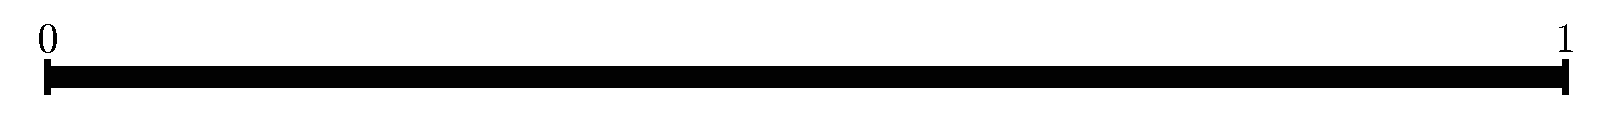
\includegraphics[trim=0cm 0cm 0cm 0cm, clip, scale=0.5]{images/Cantor0.pdf}
	\end{center}
	\item \textbf{Passo 1.} Suddividiamo $\left[0,1\right]$ in tre sottointervalli di ugual lunghezza
	\begin{equation*}
		I_1=\left[0,\nicefrac{1}{3}\right]\qquad I_2=\left(\frac{1}{3},\nicefrac{2}{3}\right)\qquad I_3=\left[\frac{2}{3},1\right]
	\end{equation*}
	e rimuoviamo l'intervallo aperto intermedio $I_2$, lasciando gli intervalli $I_1$ e $I_2$.
	\begin{center}
		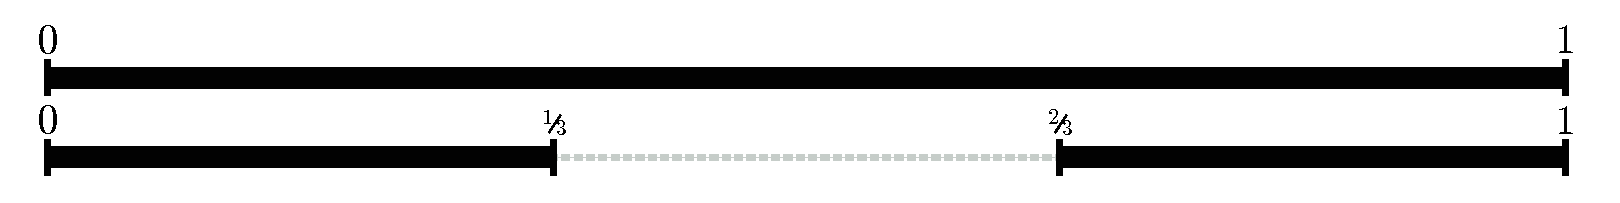
\includegraphics[trim=0cm 0cm 0cm 0cm, clip, scale=0.5]{images/Cantor1.pdf}
	\end{center}
	\item \textbf{Passo 2.} Prendiamo ciascun intervallo che avevamo al passo 1 e lo suddividiamo in modo analogo in tre parti uguali; per ciascun intervallo eliminiamo il sottointervallo aperto centrale, lasciando dunque 4 intervalli di lunghezza $\nicefrac{1}{9}$.
	\begin{center}
		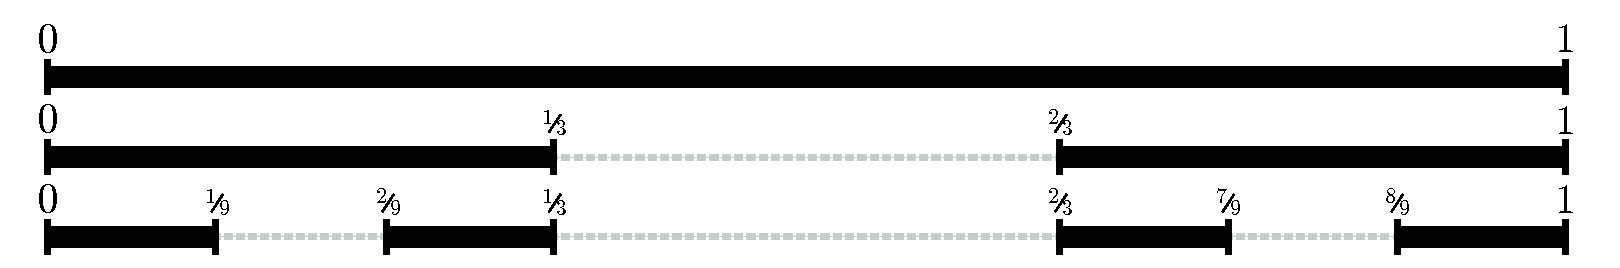
\includegraphics[trim=0cm 0cm 0cm 0cm, clip, scale=0.5]{images/Cantor2.pdf}
	\end{center}
	\item \textbf{Passo 3 e successivi.} Ripetiamo il procedimento del passo 2 con gli intervalli ottenuti nel passaggio precedente.
\begin{center}
	
\includegraphics[trim=0cm 0cm 0cm 0cm, clip, scale=0.5]{images/Cantor3.pdf}
\end{center}
\end{itemize}
I punti che rimangono dopo infiniti passi è noto come \textbf{insieme di Cantor}\index{insieme!di Cantor} $C$.
\begin{equation*}
	C=\left[0,1\right]\setminus\bigcup_{n=0}^\infty \bigcup_{k=0}^{3^n-1} \left(\frac{3k+1}{3^{n+1}},\frac{3k+2}{3^{n+1}}\right)
\end{equation*}
Ci si potrebbe chiedere se ci sono ancora dei punti in questo insieme: dopotutto, abbiamo rimosso e rimosso continuamente degli intervalli. Sorprendentemente, dopo infiniti di questi passi ci sono ancora punti che rimangono, ma la peculiarità è che sono addirittura \textbf{non numerabili}!
\begin{theorema}[Innumerabilità dell'insieme di Cantor]
	Si denoti con $C$ l'insieme ternario di Cantor. Esiste una funzione suriettiva da $C$ in $\left[0,1\right]$; conseguentemente, $C$ ha la cardinalità del continuo.
\end{theorema}
\begin{demonstration}
	Ricordiamo che per ogni numero $x\in [0,1]$ esiste una successione $\{i_n\}_{n\geq 1}$ di interi, con $i_n\in \{0, 1, 2\}$, tale che 
	\begin{equation*}
		x=\sum_{n=1}^{+\infty} \dfrac{i_n}{3^n}. 
	\end{equation*}
	Tale successione è unica, tranne quando $x$ è della forma $q/3^n$, con  $q\in \naturalset$, nel qual caso esistono esattamente due successioni. Descriviamo l'insieme di Cantor $C$ usando questa rappresentazione in \textit{base tre}.
	\begin{itemize}
		\item Osserviamo che $\nicefrac{1}{3}$ si scrive come $0.1_3$ e $\nicefrac{2}{3}$ si scrive come $0.2_3$. Il \textit{primo intervallo} rimosso nella costruzione dell'insieme di Cantor consiste quindi di tutti i numeri del tipo $0.1abc\ldots_3$, dove $abc\ldots$ è una qualsiasi sequenza di numeri diversi dalle sequenze estreme $0000\ldots$ e $222\ldots$. I numeri residui dopo il primo passo della costruzione di $C$ sono esattamente quelli scrivibili come $0.0abc\ldots_3$ e $0.2abc\ldots_3$.
		\item Al secondo passo si rimuovono tutti i numeri del tipo $0.01abc\ldots_3$ e $0.21abc\ldots_3$.
	\end{itemize}
	Segue che i numeri che non vengono mai rimossi e che quindi appartengono all'insieme $C$ sono esattamente quelli che possono essere scritti come $0.abc\ldots_3$ usando solo le cifre $0$ e $2$.\\
	Definiamo ora una funzione $\funz{f}{C}{\left[0,1\right]}$ associando ad ogni elemento di $C$ scritto come $0.abc\ldots_3$, dove le cifre decimali sono solo $0$ e $2$, il numero di $\left[0,1\right]$ la cui rappresentazione in base due è quella ottenuta dalla sequenza $0.abc\ldots$ sostituendo ogni cifra $2$ con la cifra $1$.\\
	La funzione $f$ è chiaramente suriettiva: dato un numero $x\in \left[0,1\right]$, la sua controimmagine mediante $f$ è l'elemento dell'insieme di Cantor la cui rappresentazione decimale ternaria si ottiene dalla rappresentazione binaria di $x$ sostituendo ogni cifra $1$ con la cifra $2$.\\
	L'esistenza di una funzione suriettiva da $C$ in $\left[0,1\right]$ implica\footnote{In ‘‘Brevi cenni di teoria degli insiemi'', a pag. \pageref{cardinalitàsuriettiva} è possibile trovare maggiori dettagli su questa proprietà.} che la cardinalità di C è maggiore o uguale a quella di $\left[0,1\right]$:
	\begin{equation*}
		\abs{C}\geq \abs{X} 
	\end{equation*}
	D'altra parte, $C\subseteq \left[0,1\right]$ e dunque\footnote{In ‘‘Brevi cenni di teoria degli insiemi'', a pag. \pageref{cardinalitàinclusione} è possibile trovare maggiori dettagli su questa proprietà.} la sua cardinalità è minore o uguale a quella di $\left[0,1\right]$.
	\begin{equation*}
		\abs{C}\leq\abs{X}
	\end{equation*}
	Concludiamo quindi che $C$ e $\left[0,1\right]$ hanno la stessa cardinalità e dunque $C$ ha la cardinalità del continuo $\mathfrak{c}$.
\end{demonstration}
\begin{digression}
	Si noti che l'insieme di Cantor è un \textbf{frattale}\index{frattale}, dato che è sempre uguale a due copie di se stesso, se ogni copia è ristretta di un terzo e traslata.
\end{digression}
Pur essendo non numerabile esso ha lunghezza nulla. Nello specifico, consideriamo la misura di Lebesgue $m_1$ e ripercorriamo i passaggi della costruzione dell'insieme di Cantor:
\begin{itemize}
	\item \textbf{Passo 0.} $C_0$ coincide con l'intervallo $\left[0,1\right]$:
	\begin{equation*}
		m_1\left(C_0\right)=1
	\end{equation*}
	\item \textbf{Passo 1.} Togliamo un segmento di lunghezza $\nicefrac{1}{3}$ da un segmento di lunghezza $1$:
	\begin{equation*}
		m_1\left(C_1\right)=m_1\left(C_0\right)-\frac{1}{3}=\frac{2}{3}
	\end{equation*}
	\item \textbf{Passo 2.} Togliamo dei segmenti di lunghezza complessiva $\nicefrac{2}{9}$ da un'unione di segmenti di lunghezza $\nicefrac{2}{3}$:
	\begin{equation*}
		m_1\left(C_2\right)=m_1\left(C_1\right)-\frac{2}{9}=\frac{2}{3}-\frac{2}{9}=\frac{4}{9}
	\end{equation*}
\end{itemize}
Ad ogni passo l'insieme ha sempre lunghezza $\nicefrac{2}{3}$ quello del precedente. Al passo $n$-esimo si ha
\begin{equation*}
	m_1\left(C_n\right)=\left(\frac{2}{3}\right)^n
\end{equation*}
Poiché l'insieme di Cantor è prodotto dopo infiniti passi, allora
\begin{equation*}
	m_1\left(C\right)=\lim_{n\to+\infty}m_1\left(C_n\right)=\lim_{n\to+\infty}\left(\frac{2}{3}\right)^n=0
\end{equation*}
\subsection{Regolarità della misura di Lebesgue}
Ora enunciamo una proprietà della misura di Lebesgue, detta \textbf{regolarità}\index{regolarità!della misura di Lebesgue}.
\begin{theorema}[Regolarità della misura di Lebesgue]\label{regolaritàlebesgue}
	Le seguenti affermazioni sono equivalenti:
	\begin{enumerate}
		\item $E\in\mathcal{L}\left(\realset^n\right)$.
		\item $\forall \epsilon > 0,\ \exists A_{\epsilon}$ aperto di $\realset^n$ tale che
		\begin{itemize}
			\item $E\subseteq A_{\epsilon}$.
			\item $m^{X}_n\left(A_{\epsilon}\setminus E\right)<\epsilon$.
		\end{itemize}
		\item $\exists B$ Boreliano di $\realset^n$ tale che
	\begin{itemize}
		\item $E\subseteq B$.
		\item $m^{X}_n\left(B\setminus E\right)=0$.
	\end{itemize}
	\item $\forall \epsilon > 0,\ \exists C_{\epsilon}$ chiuso di $\realset^n$ tale che
	\begin{itemize}
		\item $E\supseteq C_{\epsilon}$.
		\item $m^{X}_n\left(E\setminus C_{\epsilon}\right)<\epsilon$.
	\end{itemize}
	\item $\exists D$ Boreliano di $\realset^n$ tale che
	\begin{itemize}
		\item $E\supseteq D$.
		\item $m^{X}_n\left(E\setminus D\right)=0$.
	\end{itemize}~\\
	\begin{minipage}{0.4\textwidth}
	\begin{center}
		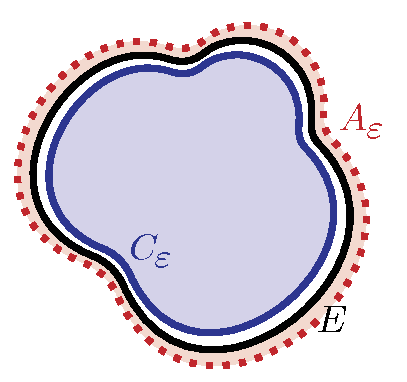
\includegraphics[trim=0cm 0cm 0cm 0cm, clip, scale=0.7]{images/regolarita1}\\
		\textbf{Caso 2. + 4.}
	\end{center}
\end{minipage}
\begin{minipage}{0.5\textwidth}
	\begin{center}
			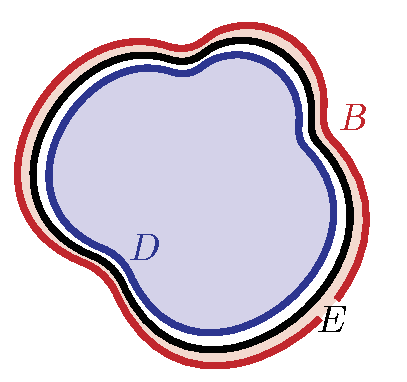
\includegraphics[trim=0cm 0cm 0cm 0cm, clip, scale=0.7]{images/regolarita2}\\
			\textbf{Caso 3. + 5.}
	\end{center}
\end{minipage}
	\end{enumerate}
\end{theorema}
\begin{demonstration}
	Dimostriamo le catene di implicazioni
	\begin{equation*}
		\mathbf{(i)\implies (ii)\implies (iii)\implies (i)\qquad(i)\implies (iv)\implies (v)\implies (i)}
	\end{equation*}
$\mathbf{(i)\implies(ii)}\quad$ Consideriamo il caso $m_n(E)<+\infty$. Per definizione di $m^{X}_n$ e di $\inf$, fissato $\epsilon >0$ $E$ è contenuto in un ricoprimento di parallelepipedi aperti tale che
\begin{equation*}
	\sum_{i=1}^{+\infty}V_n\left(P_i\right)<m_n(E)+\epsilon
\end{equation*}
dunque, posto
\begin{equation*}
	A=\bigcup_{n\in\naturalset}P_n,
\end{equation*}
l'aperto $A$ verifica, per subadditività numerabile,
\begin{equation*}
	m_n\left(A\right)<m_n(E)+\epsilon
\end{equation*}
e dal fatto che $m_n(E)<+\infty$ segue allora % aggiungere tabella proprietà in footnotes
\begin{equation*}
	m_n\left(A\setminus E\right)=m_n\left(A\right)-m_n(E)<\epsilon
\end{equation*}
Sia ora $m_n(E)=+\infty$. Possiamo vederlo come la seguente unione:
\begin{equation*}
	E=\bigcup_{i=1}^{+\infty}\left(E\cap Q_i\right),
\end{equation*}
dove $Q_i$ è una famiglia di parallelepipedi privi di punti interni comuni (ossia che hanno in comune al più i bordi), la cui unione sia $\realset^n$. Dato che $m_n\left(E\cap Q_n\right)<m_n(E)<Q$, per quanto già dimostrato esistono degli $A_i\supseteq E\cap Q_i$ tali che
\begin{equation*}
	m_n\left(A_i\setminus\left(E\cap Q_i\right)\right)<\frac{\epsilon}{2^{i+1}},\ \forall i\in\naturalset
\end{equation*}
Allora possiamo prendere come aperto
\begin{equation*}
	A=\bigcup_{i=1}^{+\infty}A_i.
\end{equation*}
Esso contiene $E$, e poiché
\begin{equation*}
	A\setminus E=\left(\bigcup_{i=1}^{+\infty}A_i\right)\setminus\left(\bigcup_{i=1}^{+\infty}\left(E\cap Q_i\right)\right)\subseteq\bigcup_{i=1}^{+\infty}\left(A_i\setminus\left(E\cap Q_i\right)\right)
\end{equation*}
si conclude che
\begin{equation*}
	m_n\left(A\setminus E\right)<\sum_{i=1}^{+\infty}m_n\left(A_i\setminus\left(E\cap Q_i\right)\right)<\epsilon
\end{equation*}
$\mathbf{(ii)\implies(iii)}\quad$ Per ogni $i\in\naturalset$, sia $A_i$ un aperto contenente $E$, tale che
\begin{equation*}
	m^{X}_n\left(A_i\setminus E\right)<\frac{1}{i+1}.
\end{equation*}
L'insieme
\begin{equation*}
	B=\bigcap_{i=1}^{+\infty}A_i
\end{equation*}
è un Boreliano contenente $E$ e si ha, per monotonia,
\begin{equation*}
	m_n^{X}\left(B\setminus E\right)\leq m_n^{X}\left(A_i\setminus E\right)<\frac{1}{n+1},\ \forall i\in \naturalset
\end{equation*}
cioè $m_n^{X}\left(B\setminus E\right)=0$.\\
$\mathbf{(iii)\implies(i)}\quad$  Scrivendo $E=B\setminus\left(B\setminus E\right)$, la tesi segue dal fatto che l'insieme $B$ è misurabile perché boreliano, mentre l'insieme $B\setminus E$ è misurabile avendo, per ipotesi, misura esterna nulla. Dunque $E$ è misurabile.\\
$\mathbf{(i)\implies(iv)\implies(v)\implies(i)}\quad$ Queste implicazioni si dimostrano facilmente applicando ad $E^C$ gli enunciati già dimostrati. 
\end{demonstration}
\begin{observe}
	Dai punti 2 e 4 si può caratterizzare un insieme $E$ misurabile secondo Lebesgue come un insieme che \textit{differisce poco}, in termini della misura esterna, sia da aperti contenenti $E$, sia da chiusi contenuti in $E$.\\
	Dai punti 3 e 5, invece, si può vedere ogni insieme misurabile secondo Lebesgue come un Boreliano a cui abbiamo tolto o aggiunto, rispettivamente, un insieme di misura nulla. Nello specifico, dal punto 5,
	\begin{equation*}
		E=D\cup\left(E\setminus D\right)
	\end{equation*}
\end{observe}
\subsection{Confronto tra la misura di Peano-Jordan e di Lebesgue}
Come abbiamo visto, la misura di Peano-Jordan soddisfa solo alcune proprietà della misura in senso assiomatico, essendo $\sigma$-subadditiva, mentre la misura secondo Lebesgue è a tutti gli effetti una misura assiomatica moderna. Ci si può dunque chiedere se tali concetti sono incompatibili tra di loro oppure se c'è una qualche relazione tra di esse.\\
È già noto che non tutti gli insiemi misurabili secondo Lebesgue lo sono secondo Peano-Jordan.
\begin{example}
	Consideriamo $E=\rationalset\cap\left[0,1\right]$.
	\begin{itemize}
		\item $E$ numerabile implica che $E$ è Lebesgue-misurabile e $m_1(E)=0$.
		\item $E$ \textit{non} è Peano-Jordan misurabile, in quanto
		\begin{equation*}
			m_{PJ}^{X}(E)=1\neq 0=m_{PJ,X}(E)
		\end{equation*}
	\end{itemize}
\end{example}
Invece, si vede banalmente che gli insiemi elementari, ossia le unioni di parallelepipedi $n$-dimensionali, sono misurabili sia secondo Lebesgue, sia secondo Peano-Jordan (a patto di fare un'unione finita di elementi); in particolare, le misure coincidono.
\begin{gather*}
	m_{PJ}(P)=m_n(P)=V_n(P)\\
	m_{PJ}\left(\bigcup_{i=1}^{k}P_i\right)=m_n\left(\bigcup_{i=1}^{k}P_i\right)=\sum_{i=1}^{k}V_n\left(P_i\right)
\end{gather*}
Il seguente teorema ci afferma un risultato importante: \textit{tutti} gli insiemi misurabili secondo Peano-Jordan sono misurabili secondo Lebesgue e le misure in tal caso coincidono.
\begin{theorema}[Misurabile secondo Peano-Jordan implica misurabile secondo Lebesgue]
	Sia $E\subseteq\realset^n$ limitato. Allora
	\begin{enumerate}
		\item Se $E$ è Peano-Jordan misurabile allora $E$ è Lebesgue-misurabile.
		\item Se vale ciò, allora $m_{PJ}(E)=m_n(E)$.
	\end{enumerate}
\end{theorema}
\begin{demonstration}
	Dimostriamo il punto 1. Sia $E\subseteq \realset^n$ e Peano-Jordan misurabile. Per provare che $E$ è misurabile secondo Lebesgue useremo il teorema di \textit{regolarità} precedentemente dimostrato.\\
	In particolare, proviamo che $\forall \epsilon >0\ \exists A_{\epsilon}$ aperto tale che
	\begin{itemize}
		\item $E\subseteq A_{\epsilon}$.
		\item $m_n^{X}\left(A_{\epsilon}\setminus E\right)<\epsilon$.
	\end{itemize}
Sappiamo che $E$ è misurabile secondo Peano-Jordan, dunque per il criterio equivalente $\forall \epsilon >0,\ \exists A_{\epsilon},\ B_{\epsilon}$ unioni finite di parallelepipedi con $B_{\epsilon}\subseteq E\subseteq A_{\epsilon}$ tali che $m_{PJ}\left(A_{\epsilon}\setminus B_{\epsilon}\right)<\epsilon$. Allora l'insieme $A_{\epsilon}$ così definito è proprio quello che stavamo cercando. Noto innanzitutto che $A_{\epsilon}\setminus E\subseteq A_{\epsilon}\setminus B_{\epsilon}$, per monotonia della misura esterna otteniamo:
\begin{equation*}
	m_{n}^{X}\left(A_{\epsilon}\setminus E\right)<	m_{n}^{X}\left(A_{\epsilon}\setminus B_{\epsilon}\right)=m_{PJ}^X\left(A_{\epsilon}\setminus B_{\epsilon}\right)=m_{PJ}\left(A_{\epsilon}\setminus B_{\epsilon}\right)<\epsilon\qedhere
\end{equation*}
\end{demonstration}
\section{Definizione assiomatica di misura}
La definizione di misura di Lebesgue che abbiamo analizzato nella scorsa sezione non è esattamente la stessa che il matematico francese diede nella sua tesi di laurea, bensì una rielaborazione successiva con alcune modifiche; nello specifico, la trattazione moderna viene inquadrata nella teoria \textbf{assiomatica} della misura, introdotta già prima di Lebesgue da Emil \textbf{Borel} (1871-1956) in \textit{Léçons sur la théorie des fonctions (1898)}.\\
I concetti di $\sigma$-algebra e insieme misurabile che abbiamo già affrontato si possono ricondurre proprio a Borel, così come la seguente \textit{definizione assiomatica} di misura.
\begin{define}[Misura e spazio di misura]
	Dato $\left(X,\mathcal{M}\right)$ uno spazio misurabile, una funzione $\funz{\mu}{\mathcal{M}}{\realset^{\ast}=\left[-\infty,+\infty\right]}$ è detta \textbf{misura}\index{misura} se soddisfa le seguenti proprietà:
	\begin{itemize}
		\item \textsc{\textbf{Non negatività:}} $\forall A\in\mathcal{M},\ \mu\left(A\right)\geq 0$.
		\item \textsc{\textbf{Insieme vuoto nullo:}} $\mu\left(\emptyset\right)=0$.
		\item $\sigma$-\textsc{\textbf{additività:}} $\forall A_n\in\mathcal{M}$ tali che $A_i\cap A_j=\emptyset\ \forall i\neq j$, allora
		\begin{equation}
			\mu\left(\coprod_{n\geq 1}A_n\right)=\sum_{n\geq 1}\mu\left(A_n\right)
		\end{equation}
	\end{itemize}
	In tal caso la terna $\left(X,\mathcal{M},\mu\right)$ è detta \textbf{spazio di misura}\index{spazio!di misura}.
	\begin{itemize}
		\item $\mu$ si dice \textbf{completa}\index{misura!completa} se $\forall S\subseteq N,\ \forall N\in\mathcal{M}\colon\mu(N)=0\implies S\in\mathcal{M}$ e $\mu(S)=0$.
		\item $\mu$ si dice \textbf{finita}\index{misura!finita} se $\mu(x)<+\infty$.
		\item $\mu$ si dice $\sigma$-\textbf{finita}\index{misura!$\sigma$-finita} se
		\begin{itemize}
			\item $\mu(x)=+\infty$.
			\item $\displaystyle X=\bigcup_{n\geq 1}X_n$, con $X_n\in\mathcal{M}$ tale che $\mu\left(X_n\right)\leq +\infty$.
		\end{itemize}
	\item $\mu$ si dice \textbf{di probabilità}\index{misura!di probabilità} se $\mu(x)=1$.
	\end{itemize}
\end{define}
\begin{observe}
	Ogni misura può essere opportunamente essere resa completa estendendo la $\sigma$-algebra di definizione.
\end{observe}
\begin{exampleswt}[Spazi di misura]~{}
	\begin{enumerate}
		\item $\left(\realset^n,\mathcal{L}\left(\realset^n\right)\right)$ è spazio di misura con la \textbf{misura di Lebesgue}
		\begin{equation}
			\funz{m_n}{\mathcal{L}\left(\realset^n\right)}{\left[0,+\infty\right]}
		\end{equation}
		Osserviamo che $m_n$ è $\sigma$-finita perché $m_n\left(\realset^n\right)=+\infty$ con
		\begin{equation*}
			\realset^n=\bigcup_{n\geq 0}B_n\left(0\right)\quad\text{con }m_n\left(B_n\left(0\right)\right)<+\infty
		\end{equation*}
		Inoltre, essa è \textbf{completa}. % to do: aggiungere dim completa?
		\item Fissato $x_0\in X$ insieme qualunque, $\left(X,\setpart{X}\right)$ è uno spazio di misura con la funzione $\delta$ \textbf{di Dirac concentrata in} $x_0$\index{Delta di Dirac}:
		\begin{equation}
			\funztot{\delta}{\setpart{X}}{\left[0,+\infty\right]}{E}{\begin{cases}
					\begin{array}{ll}
						1&\text{se }x_0\in E\\
						0&\text{se }x_0\notin E
					\end{array}
			\end{cases}}
		\end{equation}
		\item Preso $X$ insieme qualunque e scelti
		\begin{itemize}
			\item $\left\{x_n\right\}_{n\geq 0}$ una famiglia di elementi di $X$.
			\item $p_n\geq 0, \forall n\geq 0$ dei \textbf{pesi}\index{peso}.
		\end{itemize}
	allora $\left(X,\setpart{X}\right)$ è spazio di misura con la \textbf{misura di conteggio pesata}\index{misura!di conteggio!pesata}:
	\begin{equation}
		\funztot{\mu}{\setpart{X}}{\left[0,+\infty\right]}{E}{\displaystyle\sum_{n\colon x_n\in E}p_n}
	\end{equation}
Se
\begin{equation*}
	\sum_{n\colon x_n\in E}p_n=1,
\end{equation*}
$\mu_p$ è una \textbf{misura di probabilità discreta}\index{misura!di probabilità!discreta}, come la m.d.p. \textit{binomiale}, di \textit{Poisson}, ecc...\\
\item Preso $X=\naturalset$, i punti $x_n=n, \forall n\geq 1$ e $p_n=1,\ \forall n\geq 1$, allora $\left(\naturalset,\setpart{\naturalset}\right)$ è spazio di misura con la \textbf{misura di conteggio semplice}\index{misura!di conteggio!semplice}, un caso particolare dell'esempio precedente:
	\begin{equation}
	\forall E\subseteq\naturalset,\ \mu(E)=\sum_{n\colon n\in E}1=\begin{cases}
		\begin{array}{ll}
			\# E&\text{se }E\text{ finito}\\
			+\infty&\text{se }E\text{ infinito}
		\end{array}
	\end{cases}
\end{equation}
	\end{enumerate}
\end{exampleswt}
\begin{property}[Continuità della misura]
	Sia $\left(X,\mathcal{M}\right)$ uno spazio misurabile, $\funz{\mu}{\mathcal{M}}{\left[0,+\infty\right]}$ una misura. Allora $\mu$ è una funzione \textbf{continua da sopra e da sotto} - dove la continuità è quella delle funzioni definite su una collezione di insiemi:
	\begin{itemize}
		\item Per ogni successione di insiemi $A_n$ \textit{crescente}, cioè tale che $A_i\subseteq A_{i+1},\ \forall i\in\naturalset$, si ha
		\begin{equation}
			\mu\left(\bigcup_{n\geq 1}A_n\right)=\lim_{n\to+\infty}\mu\left(A_n\right)
		\end{equation}
		e $\mu$ è detta \textbf{continua da sotto}\index{continuità!da sotto}. 
	\begin{center}
		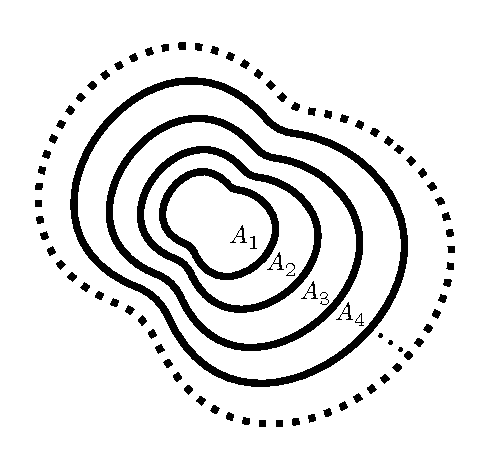
\includegraphics[trim=0cm 0cm 0cm 0cm, clip, scale=0.6]{images/misuracontinua1.pdf}
	\end{center}
	\item Per ogni successione di insiemi $A_n$ \textit{decrescente}, cioè tale che $A_{i+1}\subseteq A_i,\ \forall i\in\naturalset$, con $\mu(A_1)<+\infty$, si ha
		\begin{equation}
			\mu\left(\bigcap_{n\geq 1}A_n\right)=\lim_{n\to+\infty}\mu\left(A_n\right)
		\end{equation}
	e $\mu$ è detta \textbf{continua da sopra}\index{continuità!da sopra}.
	\begin{center}
		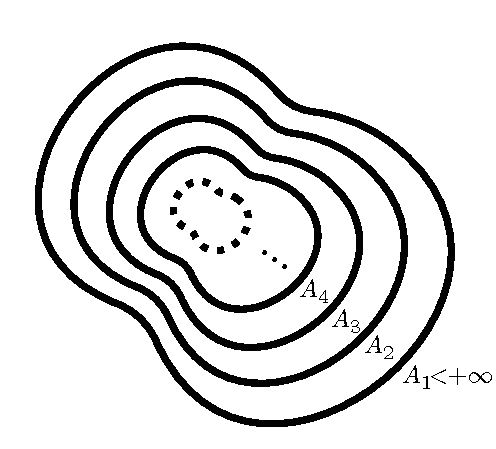
\includegraphics[trim=0cm 0cm 0cm 0cm, clip, scale=0.6]{images/misuracontinua2.pdf}
	\end{center}
	\end{itemize}
\end{property}
\begin{attention}
	Per la continuità da sopra è fondamentale l'ipotesi che $\mu\left(A_1\right)$ è finita.
\end{attention}
\begin{examplewt}[Controesempio alla continuità da sopra]
	Consideriamo la misura di Lebesgue unidimensionale $m_1$ e prendiamo la successione $A_n=\left[n,+\infty\right)$. Essa è decrescente in quanto
	\begin{equation*}
		A_{n+1}=\left[n+1,+\infty\right)\subsetneqq\left[n,+\infty\right)=A_n.
	\end{equation*}
	Si ha $m\left(A_n\right)=+\infty,\ \forall n$, e quindi in particolare
	\begin{equation*}
		\lim_{n\to+\infty}\mu\left(A_n\right)=+\infty
	\end{equation*}
	D'altro canto si ha
	\begin{equation*}
		\bigcap_{n\geq 1}A_n=\emptyset\implies\mu\left(\bigcap_{n\geq 1}A_n\right)=\mu\left(\emptyset\right)=0
	\end{equation*}
\end{examplewt}
\section{Famiglie di insiemi nella teoria della misura e relazioni tra di loro}\label{famigliediinsiemi}
Concludiamo questo capitolo alcune delle più comuni \textit{famiglie di insiemi} che si incontrano nello studio della teoria della misura.
\begin{center}
	\begin{tabular}{c|c|c}
		\textbf{Nome}                                                                            & \textbf{Notazione}                          & \textbf{Cardinalità}        \\ \hline
		Insieme delle parti                                                             & $\setpart{\realset}$               & $2^{\mathfrak{c}}$ \\ \hline
		\begin{tabular}[c]{@{}c@{}}Insiemi misurabili\\ (secondo Lebesgue)\end{tabular} & $\mathcal{L}\left(\realset\right)$ & $2^{\mathfrak{c}}$ \\ \hline
		Boreliani                                                                      & $\mathcal{B}\left(\realset\right)$ & $\mathfrak{c}$     \\ \hline
		\begin{tabular}[c]{@{}c@{}}Topologia\\ (famiglia degli aperti)\end{tabular}     & $\topo$                            & $\mathfrak{c}$    
	\end{tabular}
\end{center}
\begin{proposition}[Relazioni tra classi di insiemi]
	Valgono le seguenti inclusioni:
	\begin{equation}
		\topo\subsetneqq\mathcal{B}\left(\realset\right)\subsetneqq\mathcal{L}\left(\realset\right)\subsetneqq\setpart{\realset}
	\end{equation}
\end{proposition}
Mostreremo alcune di queste inclusioni in modo formale, mentre per altre daremo solo un'intuizione della dimostrazione.
\paragraph{Cardinalità dell'insieme delle parti dei reali}
Se $\abs{\realset}=\mathfrak{c}$ è la cardinalità del continuo, allora la cardinalità dell'\textit{insieme delle parti dei reali}\footnote{In ‘‘Brevi cenni di teoria degli insiemi'', a pag. \pageref{cardinalitàsetpart} è possibile trovare qualche dettaglio sulla cardinalità dell'insieme delle parti di un insieme e a pag. \pageref{cardinalitàsetpartreali} su quella dell'insieme delle parti dei reali.} è
\begin{equation}
	\abs{\setpart{\realset}}=2^{\mathfrak{c}}
\end{equation}
\paragraph{Cardinalità degli insiemi misurabili}
Per trovare quanti sono gli insiemi misurabili, consideriamo l'\textit{insieme di Cantor} $C$. Abbiamo visto\footnote{Si veda pag. \pageref{insiemecantor}.} che esso gode delle seguenti proprietà:
\begin{enumerate}
	\item Il numero di punti prima e dopo il processo iterativo per costruire $C$ rimane invariato, dunque $C$ è \textit{non numerabile} e ha la stessa cardinalità di $\left[0,1\right]$:
	\begin{equation*}
		\abs{C}=\abs{\left[0,1\right]}=\mathfrak{c}
	\end{equation*}
	\item $C$ è misurabile e $m_1\left(C\right)=0$.
\end{enumerate}
Dal punto 1 segue che l'insieme delle parti dell'insieme di Cantor ha cardinalità $\setpart{C}=2^{\mathfrak{c}}$, mentre dal punto 2 si può dedurre che ogni sottoinsieme di $C$ ha misura nulla ed è pertanto misurabile. Insiemisticamente parlando, le relazioni sono
\begin{equation*}
	\setpart{C}\subseteq \mathcal{L}\left(\realset\right)\subseteq\setpart{\realset}
\end{equation*}
Passando alle cardinalità:
\begin{equation*}
	2^{\mathfrak{c}}\underset{(1)}{=}{\abs{\setpart{C}}}\leq \abs{\mathcal{L}\left(\realset\right)}\leq\abs{\setpart{\realset}}=2^{\mathfrak{c}}\implies \abs{\mathcal{\realset}}=2^{\mathfrak{c}}
\end{equation*}
\paragraph{Inclusione stretta di {$\mathcal{L}\left(\realset\right)$} in {$\setpart{\realset}$}}
Il fatto che la cardinalità degli insiemi Lebesgue-misurabili in $\realset$ coincida con quella dell'insieme delle parti di $\realset$ non è sufficiente\footnote{Si veda ‘‘Brevi cenni di teoria degli insiemi'', pag. \pageref{cardinalitàugualenonimplicauguaglianzainsiemistica}.} per affermare che i due insiemi coincidano; costruiamo ora un sottoinsieme particolare di $\realset$ che risulta \textit{non misurabile}.
\begin{define}[Insieme di Vitali]\label{vitali}.
	Considerata in $\realset$ la relazione di equivalenza
	\begin{equation}
		x\sim y\iff x-y\in\rationalset
	\end{equation}
	possiamo definire delle classi di equivalenza in $\nicefrac{\realset}{\sim}$:
	\begin{align*}
		\left[0\right]&=\left\{0,1,\frac{1}{2},-\frac{3}{4},\frac{123}{72},\ldots\right\}=\left\{x\in\realset\mid x\in\rationalset\right\}=\rationalset\\
		\left[\sqrt{2}\right]&=\left\{\sqrt{2},\sqrt{2}+\frac{1}{2},\sqrt{2}-1,\ldots\right\}=\left\{x\in\realset\mid x=\sqrt{2}+q,\ q\in\rationalset\right\}\\
		\left[\pi\right]&=\left\{\pi,\pi-\frac{3}{4},\pi+23,\ldots\right\}=\left\{x\in\realset\mid x=\pi+q,\ q\in\rationalset\right\}\\
		\vdots
	\end{align*}
	Scelto\footnote{Per poter fare questa operazione è necessario supporre l'\textit{Assioma di Scelta}.} un elemento che stia in $\left[0,1\right]$ da ogni classe di equivalenza, definisco l'\textbf{insieme di Vitali}\index{insieme!di Vitali} $V$ come unione di questi elementi.
\end{define}
Per costruzione $V\subseteq\left[0,1\right]$. Preso l'insieme \textit{numerabile} $\rationalset\cap\left[0,1\right]$, possiamo prendere una sua \textit{numerazione} $\left\{q_n\right\}$ e definire delle \textit{traslazioni} dell'insieme di Vitali $V$:
\begin{equation*}
	V_n=V+q_n\subseteq\left[-1,2\right]
\end{equation*}
\begin{lemming}[Lemma 1 di Vitali - gli insiemi di Vitali traslati sono 2 a 2 disgiunti]
	Dato l'insieme di Vitali $V$  e una enumerazione $\left\{q_n\right\}$  di $\rationalset\cap\left[0,1\right]$, allora $V_n\cap V_m=\emptyset,\ \forall n\neq m$.
\end{lemming}
\begin{demonstration}
	Consideriamo $x\in V_n\cap V_m$: questo implica che $x\in V_n$ e $x\in V_m$, ossia
	\begin{equation*}
		\begin{cases}
			x=y+q_n,\ y\in V,\ q_n\in\rationalset\cap\left[-1,1\right]\\
			x=z+q_m,\ z\in V,\ q_m\in\rationalset\cap\left[-1,1\right]
		\end{cases}
	\end{equation*}
	Pertanto,
	\begin{equation*}
		y+q_n=z+q_m\iff y-z=q_m-q_n\in\rationalset
	\end{equation*}
	Poichè $y$ e $z$ differiscono di un razionale, essi appartengono alla stessa classe di equivalenza in $\nicefrac{\realset}{\sim}$, ma dato che nella costruzione dell'insieme di VItali abbiamo preso\footnote{In virtù dell'\textit{Assioma di Scelta}.} uno e un solo elemento da tale classe, allora segue che $y=z$. È immediato verificare che $q_m=q_n$ e, essendo elementi numerazione, allora $n=m$. In altre parole, l'intersezione non è vuota solo se $V_n=V_m$.
\end{demonstration}
\begin{lemming}[Lemma 2 di Vitali - ogni numero reale in {$\left[0,1\right]$} appartiene ad un $V_n$ per un certo $n$:]
	Dato l'insieme di Vitali $V$ vale la seguente relazione:
	\begin{equation*}
		\left[0,1\right]\subseteq\bigcup_{n\in\naturalset}V_n
	\end{equation*}
\end{lemming}
\begin{demonstration}
	Sia $x\in\left[0,1\right]$. Poiché la relazione $\sim$ forma una partizione di $\realset$, deve esistere $y$ tale che $x-y=q\in\rationalset$; riscrivendo tale relazione si ha $x=y+q$, ossia $x=y+q_n$ per un certo $n$.
\end{demonstration}
Possiamo osservare alcune proprietà sulla base dei due lemmi appena mostrati:
\begin{itemize}
	\item \textbf{Conseguenze del lemma 1:}
	\begin{equation*}
		m\left(\bigcup_{n\in\naturalset}V_n\right)=\sum_{n\in\naturalset}m\left(V_n\right)=\sum_{n\in\naturalset}m\left(V\right)=\begin{cases}
			\begin{array}{ll}
				0&\text{se }m\left(V\right)=0\\
				+\infty&\text{se }m\left(V\right)>0
			\end{array}
		\end{cases}
	\end{equation*}
	\item \textbf{Conseguenze del lemma 2:}
	\begin{equation*}
		1=m\left(\left[0,1\right]\right)\leq m\left(\bigcup_{n\in\naturalset}V_n\right)\leq m\left(\left[-1,2\right]\right)=3
	\end{equation*}
\end{itemize}
In altre parole, si deduce che
\begin{equation*}
	1\leq \sum_{n\in\naturalset}m\left(V\right)\leq 3
\end{equation*}
ma poiché la somma di infinite copie di $m\left(V\right)$ o è $0$ o è $+\infty$ per la conseguenza del lemma 1, in nessuno dei due casi la somma sta in $\left[1,3\right]$. Pertanto, $V$ \textit{non} è misurabile, in quanto non possiamo associargli un valore $m\left(V\right)$.
\paragraph{Cardinalità dei Boreliani e inclusione stretta di {$\mathcal{B}\left(\realset\right)$} in {$\mathcal{L}\left(\realset\right)$}}
Per \textit{induzione transfinita} si dimostra che i Boreliani hanno la cardinalità del continuo.
\begin{equation}
	\abs{\mathcal{B}\left(\realset\right)}=\abs{\realset}=\mathfrak{c}
\end{equation}
Pertanto, l'inclusione $\mathcal{B}\left(\realset\right)\subsetneqq \mathcal{L}\left(\realset\right)$ è stretta.\\
Dato che utilizziamo l'induzione transfinita su insiemi costruiti sui reali, è necessario usare l'Assioma della Scelta. Tuttavia, non è l'unico metodo per per dimostrare l'inclusione stretta di $\mathcal{B}\left(\realset\right)$ in $\mathcal{L}\left(\realset\right)$; infatti, si può costruire un insieme misurabile \textit{non} Boreliano senza fare uso dell'Assioma della Scelta. Per far ciò, definiamo prima la \textit{funzione di Cantor}.
\begin{define}[Funzione di Cantor]\label{funzionecantor}
	Si consideri l'insieme ternario di Cantor $C$. La \textbf{funzione di Cantor}\index{funzione!di Cantor} $\funz{c}{C}{C}$ è definita come
	\begin{equation}
		c(x) =\begin{cases} 
			\sum_{n=1}^\infty \frac{a_n}{2^n}, &\text{se } x = \sum_{n=1}^\infty 
			\frac{2a_n}{3^n}\in C\ \mathrm{dove}\ a_n\in\{0,1\}\\
			\sup_{y\leq x,\, y\in C} c(y), &\text{se } x\in [0,1]\setminus C.\\ \end{cases}
	\end{equation}
	Equivalentemente, preso $x\in\left[0,1\right]$ si può ottenere $c(x)$ con il seguente processo:
	\begin{itemize}
		\item Esprimi $x$ in base 3.
		\item Se $x$ contiene una cifra pari ad $1$, sostituire ogni cifra che segue il primo $1$ con $0$.
		\item Sostituire tutti i rimanenti $2$ con $1$.
		\item Interpretare il risultato come un numero binario, che diventerà $c(x)$.
	\end{itemize}
\end{define}
\begin{center}
	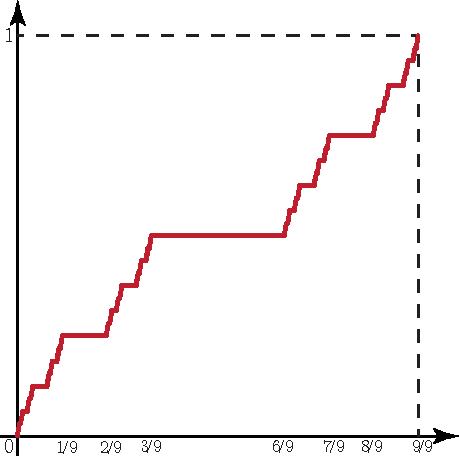
\includegraphics[width=0.4\paperwidth]{images/vasingolarecontinua}
\end{center}
Questa funzione non è altro che l'estensione della funzione $f$ incontrata nella dimostrazione dell'innumerabilità dell'insieme di Cantor ed è ben definita.\\
Si può dimostrare che $c$ è continua su $\left[0,1\right]$ ed è derivabile su $\left[0,1\right]\setminus C$ con
\begin{equation*}
	c'(x)=0,\ \forall x\in\realset\setminus C
\end{equation*}
Consideriamo ora la funzione $\funz{g}{\left[0,1\right]}{\left[0,1\right]}$ data da
\begin{equation}
	g(x)=\inf\left\{y\in\left[0,1\right]\mid c(y)=x\right\}
\end{equation}
Si ha che $g$ è una funzione iniettiva e monotona, dunque è misurabile e la controimmagine di un Boreliano tramite $g$ è ancora un Boreliano.\\
Consideriamo ora un insieme $E\subsetneqq \left[0,1\right]$ non misurabile secondo Lebesgue, dunque non è tanto meno un Boreliano. Si osservi che $F=g(E)\subseteq C$ è un insieme misurabile secondo Lebesgue perché la misura di Lebesgue è \textit{completa} ed è sottoinsieme di $C$, che ha misura nulla; tuttavia, $F$ non è un Boreliano, in quanto se lo fosse la controimmagine tramite $g$ dovrebbe essere un Boreliano, ma $g^{-1}(F)=E$, che non è però Boreliano!
% SVN info for this file
\svnidlong
{$HeadURL$}
{$LastChangedDate$}
{$LastChangedRevision$}
{$LastChangedBy$}

\chapter{Integrale di Lebesgue}
\labelChapter{integraledilebesgue}

\begin{introduction}
	‘‘Si dovrebbe sempre generalizzare.''
	\begin{flushright}
		\textsc{Carl Jacobi,} prima che Teoria delle Categorie gli facesse cambiare idea.
	\end{flushright}
\end{introduction}
\lettrine[findent=1pt, nindent=0pt]{D}{opo} aver approfondito il tema della misura, in questo capitolo ci dedicheremo integralmente a parlare del punto focale del nostro studio, l'\textbf{integrale di Lebesgue}. La definizione che daremo \textit{non} è la stessa enunciata da Lebesgue, limitata alle funzioni \textit{da valori reali a valori reali}, bensì una generalizzazione avvenuta successivamente atta ad \textit{astrarre} (da qui il termine ‘‘astratto'') il concetto di integrale a funzioni da uno spazio di misura a valori reali (estesi) o complessi; per far ciò, sarà necessario definire l'integrale in tre passi consequenziali, estendendo gradualmente (ma con certe condizioni!) la famiglia di funzioni che ammettono integrale.
\section{I tre passi dell'integrale astratto di Lebesgue}
Primo di passare ad enunciare questi passi, premettiamo un paio di osservazioni su come questa definizione si distinguerà da quella dell'\textit{integrale di Riemann}:
\begin{enumerate}
	\item La definizione si dà per funzioni definite su uno spazio di misura $\left(X,\mathcal{M},\mu\right)$, mentre per Riemann le funzioni erano definite su $\realset$ o al più su $\realset^n$.	
	\item La definizione \textit{non} richiede alcuna ipotesi sulla misura di $X$, non distinguendo neanche casi tra misura finita e misura infinita.
\end{enumerate}
Come abbiamo annunciato, la definizione viene data per \textit{passaggi successivi}, utilizzando a partire dal passo 2 i passaggi precedenti. Supponiamo sempre di considerare funzioni con dominio un generico \textit{spazio di misura} $\left(X,\mathcal{M},\mu\right)$.
\begin{itemize}
	\item \textbf{\textsc{Passo 1:}} definiamo l'integrale per funzioni $\funz{s}{X}{\left[0,+\infty\right)}$ \textbf{semplici}, misurabili e non negative.
	\item \textbf{\textsc{Passo 2:}} definiamo l'integrale per funzioni
	$\funz{f}{X}{\left[0,+\infty\right]}$ \textbf{misurabili}, non negativi.
	\item \textbf{\textsc{Passo 3:}} definiamo l'integrale per funzioni $\funz{f}{X}{\complexset}$ \textbf{misurabili} e \textbf{integrabili}.
\end{itemize}
Prima di passare ai passi qui sopra enunciati, dobbiamo definire cos'è una \textit{funzione semplice} e capire come mai sono così importanti per l'integrale di Lebesgue.
\section{Funzioni semplici}
\begin{define}[Funzione semplice]
Una funzione $\funz{s}{\left(X,\mathcal{M}\right)}{\left[0,+\infty\right)}$, con $\left(X,\mathcal{M}\right)$ spazio misurabile, è detta \textbf{semplice}\index{funzione!semplice} se la sua immagine $S(X)$ è \textit{finita}.
\end{define}
Se $s$ ha l'immagine finita di cardinalità $n$, allora esistono $n$ valori distinti $\alpha_1,\ldots,\alpha_n$  valori \textit{distinti} tali che
\begin{equation*}
	s(x)=\left\{\alpha_1,\ldots,\alpha_n\right\}
\end{equation*}
Se consideriamo $A_i=\left\{x\mid s(x)=\alpha_i\right\}=s^{-1}\left(\left\{\alpha_i\right\}\right)$, allora possiamo decomporre $s$ come ‘‘somma pesata'' delle funzioni caratteristiche degli insiemi $A_i$ nella cosiddetta \textbf{decomposizione standard di }$s$\index{decomposizione standard di una funzione semplice}:
\begin{equation}
	s=\sum_{i=1}^{n}\alpha_i\chi_{A_i}
\end{equation}
\begin{proposition}[Una funzione semplice è misurabile se e solo se le controimmagini degli {$A_i$} sono misurabili]
	Una funzione semplice $s$, scritta in decomposizione standard come
	\begin{equation*}
		s=\sum_{i=1}^{n}\alpha_i\chi_{A_i}
	\end{equation*}
	è misurabile se e solo se gli insiemi $A_i=s^{-1}\left(\left\{\alpha_i\right\}\right)$ sono misurabili, $\forall i=1,\ \ldots,\ n$. 
\end{proposition}
\begin{demonstration}
	Per definizione di funzione misurabile,
	\begin{equation*}
		\funz{s}{\left(X,\mathcal{M}\right)}{\left[0,+\infty\right)}
	\end{equation*}
	è misurabile se e solo se $\forall A\subseteq\left[0,+\infty\right)$ aperto, la controimmagine
	\begin{equation*}
		s^{-1}\left(A\right)=\bigcup_{\alpha_i\in A}s^{-1}\left(\left\{\alpha_i\right\}\right)=\bigcup_{i\colon \alpha_i\in A}A_i
	\end{equation*}
è misurabile in $X$.\\
$\impliessx$ Poiché i valori $\alpha_i$, per definizione di $s$, sono finiti, per ogni $i$ possiamo considerare un intorno aperto $U\subseteq \left[0,+\infty\right)$ di $\alpha_i$ sufficientemente piccolo da non contenere alcun $a_j,\ \forall j\neq i$. Passando alla controimmagine
\begin{equation*}
	s^{-1}\left(U\right)=\bigcup_{k\colon \alpha_k\in U}A_k=A_i
\end{equation*}
per ipotesi sulla misurabilità di $s$ si ha che $A_i$ è misurabile, $\forall i$.\\
$\impliesdx$ Preso $A\subseteq\left[0,+\infty\right)$ aperto, abbiamo visto come la controimmagine è unione finita degli $A_i$:
	\begin{equation*}
	s^{-1}\left(A\right)=\bigcup_{i\colon \alpha_i\in A}A_i
\end{equation*}
Poiché per ipotesi gli $A_i$ sono misurabili, allora $A$ è unione di insiemi misurabili e quindi è anch'esso misurabile.
\end{demonstration}
\begin{examples}~{} \label{funzionesemplice}
	\begin{enumerate}
		\item Sia $\left(X,\mathcal{M}\right)=\left(\realset,\mathcal{L}(\realset)\right)$ e consideriamo la funzione $\funz{s}{\realset}{\realset}$ come da grafico.\\
		\begin{minipage}{0.4\textwidth}
			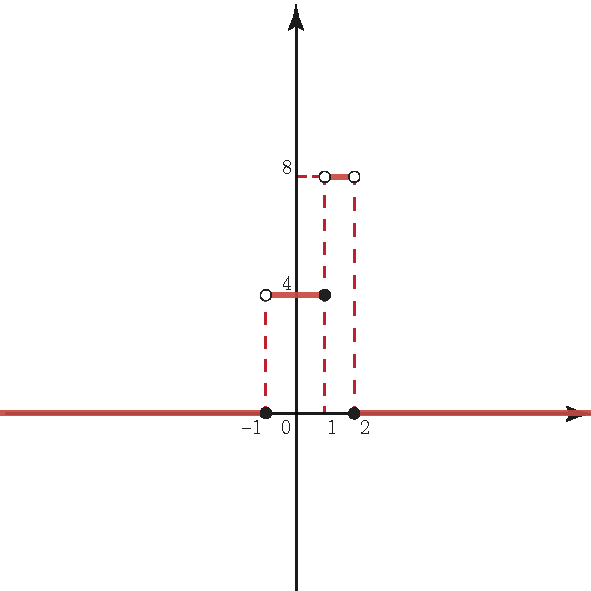
\includegraphics[trim=3cm 2cm 0cm 0cm, clip, scale=0.7]{images/graficosemplice.pdf}
		\end{minipage}\hspace{-7mm}
		\begin{minipage}{0.55\textwidth}
			Osserviamo che $s(X)=\left\{0,4,8\right\}$, dunque è semplice; le controimmagini dei valori $0$, $4$ e $8$ sono, rispettivamente:
			\begin{equation*}
				\begin{array}{l}
					A_1=s^{-1}\left(\left\{0\right\}\right)=\left(-\infty,-1\right]\cap\left[2,+\infty\right)\\
					A_2=s^{-1}\left(\left\{4\right\}\right)=\left(-1,1\right]\\
					A_3=s^{-1}\left(\left\{8\right\}\right)=\left(1,2\right)
				\end{array}
			\end{equation*}
		Pertanto la decomposizione standard di $s$ risulta
		\begin{align*}
			s&=0\chi_{\left(-\infty,-1\right]\cap\left[2,+\infty\right)}+4\chi_{\left(-1,1\right]}+8\chi_{\left(1,2\right)}=\\
			&=4\chi_{\left(-1,1\right]}+8\chi_{\left(1,2\right)}
		\end{align*}
		\end{minipage}\vspace{3mm}\\
	\item La funzione di Dirichlet
		\begin{equation*}
		s(x)=
		\begin{cases}
			\begin{array}{ll}
				1&\text{se }x\in\left[0,1\right]\cap\rationalset\\
				0&\text{se }x\in\left[0,1\right]\setminus\rationalset\\
			\end{array}
		\end{cases}
	\end{equation*}
	è semplice perché $s\left(\left[0,1\right]\right)=\left\{0,1\right\}$ e infatti $s=\chi_{\left[0,1\right]\cap\rationalset}$.
	\end{enumerate}
\end{examples}
\begin{minipage}{0.55\textwidth}
\subsection{Approssimazione di funzioni misurabili non negative con funzioni semplici}
Riprendendo l'idea di Lebesgue alla base del suo integrale, ci interessa studiare le funzioni passando attraverso la loro \textit{immagine}.\\
Si può ipotizzare di \textit{approssimare} tale funzione $f$ con una \textit{funzione semplice}: partizionando il codominio in opportuni intervalli individuati da quote fissate, se passiamo alle controimmagini possiamo sapere quali punti di $f$ sono contenuti nell'intervallo posto ad una certa quota e pertanto definire una funzione caratteristica che, come nelle \textit{carte topografiche a isoipse}, approssima la funzione $f$ per difetto.\\
Il prossimo teorema formalizza proprio questo ragionamento.
\end{minipage}\hspace{2mm}
\begin{minipage}{0.4\textwidth}
	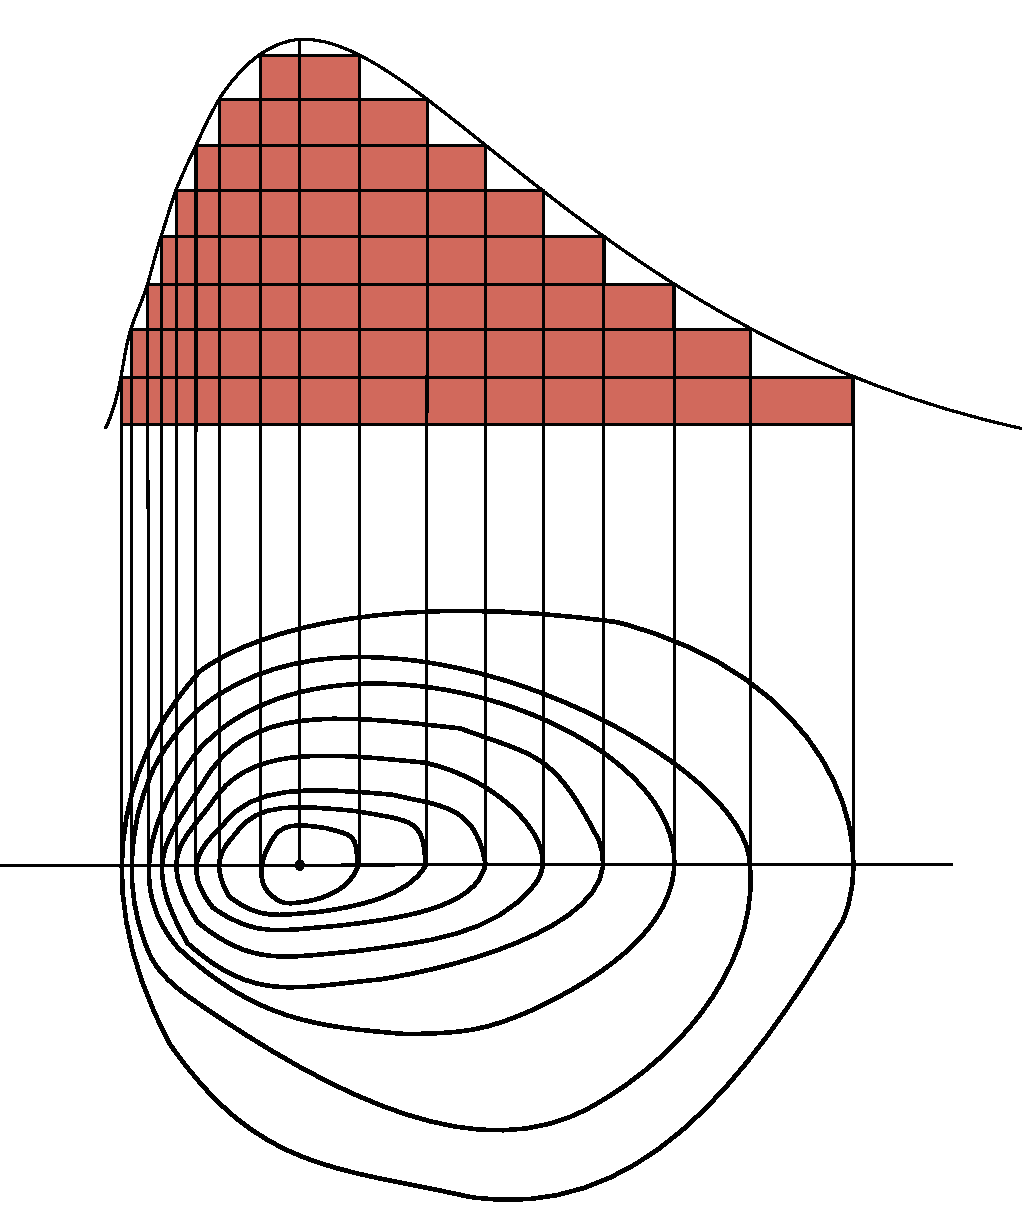
\includegraphics[trim=1cm 0cm 1.5cm 0cm, clip, scale=0.4]{images/isoipse}
\end{minipage}\vspace{3mm}\\
\begin{theorema}[Approssimazione di funzioni misurabili non negative con funzioni semplici]
	Sia $\left(X,\mathcal{M}\right)$ uno spazio misurabile e sia $\funz{f}{X}{\left[0,+\infty\right]}$ una funzione misurabile. Allora esiste una successione di funzioni semplici misurabili $\funz{s_n}{X}{\left[0,+\infty\right)}$ tale che
	\begin{itemize}
		\item $0\leq s_n(x)\leq s_{n+1}(x)\leq f(x),\ \forall x\in X,\ n\geq 1$.
		\item $\displaystyle\lim_{n\to+\infty}s_n(x)=f(x),\ \forall x\in X$.
	\end{itemize}
\end{theorema}
\begin{observe}
	La successione $s_n$ converge a $f$ puntualmente in modo \textit{monotono}.
\end{observe}
\begin{demonstration}~{}
	\begin{itemize}
		\item \textbf{\textsc{Passo 1}: costruzione della successione $s_n$ e verifica della monotonia.}\\
		Fissato $n\geq 1$, dividiamo $\left[0,+\infty\right)$ in $\left[0,n\right)$ e $\left[n,+\infty\right]$; dividiamo ulteriormente l'intervallo $\left[0,n\right)$ in $n2^n$ parti uguali
		\begin{equation*}
			\left[0,\frac{1}{2^n}\right)\quad\left[\frac{1}{2^n},\frac{2}{2^n}\right)\ldots\left[\frac{i-1}{2^n},\frac{i}{2^n}\right)\ldots\left[\frac{n2^n-1}{2^n},n\right),\ \forall i=1,\ \ldots,\ n2^n
		\end{equation*}
	Posto $E_{n,i}=f^{-1}\left(\left[\frac{i-1}{2^n},\frac{i}{2^n}\right)\right)$ e $F_n=f^{-1}\left(\left[n,+\infty\right]\right),\ \forall i=1,\ \ldots,\ n2^n$, si definisce
	\begin{equation}
		s_n=\sum_{i=1}^{n2^n}\frac{i-1}{2^n}\chi_{E_{n,i}}+n\chi_{F_n}
	\end{equation}
\begin{center}
	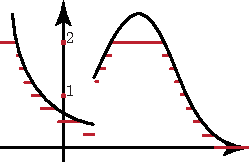
\includegraphics[trim=0cm 0cm 0cm 0cm, clip, scale=1.3]{images/approssimazione1}
\end{center}
Da questa costruzione segue che:
\begin{itemize}
	\item $s_n$ è semplice per $n$ fissato: è una combinazione lineare \textit{finita} di funzioni caratteristiche con pesi distinti.
	\item È monotona al crescere di $n$:\vspace{-3mm}
	\begin{equation*}
		0\leq s_n(x)\leq s_{n+1}(x)\leq f(x)\vspace{-3mm}
	\end{equation*}
	Intuitivamente, passando da $s_n$ a $s_{n+1}$:
	\begin{itemize}
		\item i nodi individuati in $s_n$ rimangono inalterati.
		\item vengono aggiunti dei nodi intermedi dimezzando ogni intervallino $\left[\frac{i-1}{2^n},\frac{i}{2^n}\right)$.
		\item vengono aggiunti dei nuovi nodi tra $n$ e $n+1$
	\end{itemize}
	Riducendo la dimensione di ciascun intervallino, l'approssimazione così definita risulta essere più raffinata del passo precedente; infatti, per ogni $x$ l'intervallo in cui sta ora $f(x)$ può avere lo stesso estremo inferiore che aveva con la partizione di $s_n$, oppure può avere un nuovo estremo inferiore dato da uno dei nodi introdotti con $s_{n+1}$.\\
\begin{minipage}{0.5\textwidth}
	\begin{center}
		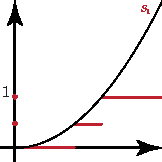
\includegraphics[trim=0cm 0cm 0cm 0cm, clip, scale=1.4]{images/approssimazione2}
	\end{center}
\end{minipage}
\begin{minipage}{0.5\textwidth}
	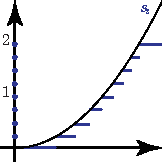
\includegraphics[trim=0cm 0cm 0cm 0cm, clip, scale=1.3]{images/approssimazione3}
\end{minipage}\vspace{4mm}
\end{itemize}
\item  \textbf{\textsc{Passo 2}: misurabilità di $s_n,\ \forall n\geq 1$.}\\
Ricordiamo che, dati $s_i\geq 0$ e $A_i\in\mathcal{M},\ i=1,\ \ldots,\ k$ si ha
\begin{equation*}
	s=\sum_{i=1}^{k}s_i\chi_{A_i}\text{ misurabile}\iff A_i\text{ misurabile},\ \forall i
\end{equation*}
Gli intervalli di $\left[\frac{i-1}{2^n},\frac{i}{2^n}\right),\ \forall i=1,\ \ldots,\ n2^n$ e $\left[n,+\infty\right)$ sono Boreliani in $\left[0,+\infty\right]$; pertanto, le controimmagini $E_{n,i}$ e $F_n$ tramite $f$ funzione misurabile sono anch'esse misurabili in $X$.
\item  \textbf{\textsc{Passo 3}: approssimazione nel senso della convergenza puntuale.}\\
	Proviamo che vale la relazione
	\begin{equation*}
		\lim_{n\to+\infty}s_n(x)=f(x),\ \forall x\in\ X
	\end{equation*}
Fissiamo $x\in X$ e distinguiamo i casi.
\begin{itemize}
	\item \textbf{\textsc{Caso 1:}} $f(x)\in\left[0,+\infty\right)$.\\
	Poiché $\floor{f(x)}\leq f(x)<\floor{f(x)}+1$, posto $N_x\coloneqq \floor{f(x)}+1$ si ha che
	\begin{equation*}
		f(x)< N_x\leq n,\ \forall n\geq N_x
	\end{equation*}
Pertanto, esiste $N_x\geq 1$ tale per cui $f(x)<n,\ \forall n\geq N_X$.\\
Sulla base di ciò si ha che $f(x)\in\left[0,n\right),\ \forall n\geq N_x$ e dunque esiste $i\in\left\{0,\ldots,n2^n\right\}$ tale per cui
\begin{equation*}
	f(x)\in\left[\frac{i-1}{2^n},\frac{i}{2^n}\right)\implies x\in f^{-1}\left(\left[\frac{i-1}{2^n},\frac{i}{2^n}\right]\right)=E_{n,i}
\end{equation*}
Allora $s_n(x)=\frac{i-1}{2^n}$ perché
\begin{gather*}
	\chi_{E_{n,j}}(x)=\delta_{i,j}\\
	\chi_{F_n}(x)\equiv 0
\end{gather*}
dove $\delta_{i,j}$ è il delta di Kronecker; segue che
\begin{equation*}
	0\leq s_n(x)=\frac{i-1}{2^n}\leq f(x)< \frac{i}{2^n}\implies 0\leq f(x)-s_n(x)<\frac{i}{2^n}
\end{equation*}
Passando al limite
\begin{equation*}
	0\leq \lim_{n\to+\infty}f(x)-s_n(x)\leq \lim_{n\to+\infty}\frac{i}{2^n}=0
\end{equation*}
Pertanto, per il \textit{teorema del confronto}
\begin{equation*}
	\lim_{n\to+\infty}f(x)-s_n(x)=0\implies \lim_{n\to+\infty}s_n(x)=f(x).
\end{equation*}
\item \textbf{\textsc{Caso 2:}} $f(x)=+\infty$.\\
Chiaramente
\begin{equation*}
	f(x)\in\left[n,+\infty\right],\ \forall n\geq 1\implies x\in f^{-1}\left(\left[n,+\infty\right]\right)=F_n
\end{equation*}
Allora $s_n(x)=n$ perché
\begin{gather*}
	\chi_{E_{n,j}}(x)\equiv 0\\
	\chi_{F_n}(x)\equiv 1
\end{gather*}
Segue che
\begin{equation*}
	\lim_{n\to+\infty}s_n(x)=\lim_{n\to+\infty}n=+\infty=f(x)\implies \lim_{n\to+\infty}s_n(x)=f(x)\qedhere
\end{equation*}
\end{itemize}
\end{itemize}
\end{demonstration}

\section{Passo 1: funzioni semplici, misurabili, non negative}
\begin{define}[Integrale di Lebesgue per funzioni semplici, misurabili, non negative]
	Sia $\funz{s}{\left(X,\mathcal{M},\mu\right)}{\left[0,+\infty\right)}$ funzione semplice, misurabile e non negativa che si decompone, dato $s(X)=\left\{\alpha_1,\ldots, \alpha_n\right\}$, nella forma standard
	\begin{equation*}
		s=\sum_{i=1}^{n}\alpha_i\chi_{A_i}\quad A_i=s^{-1}\left(\left\{A_i\right\}\right)
	\end{equation*}
	Dato $E\in\mathcal{M}$, si definisce \textit{integrale esteso a $A$ di $s$ rispetto alla misura $\mu$} il valore
	\begin{equation}
		\int_{E}sd\mu\coloneqq\sum_{i=1}^{n}\alpha_i\mu\left(A_i\cap E\right)
	\end{equation}
	con la convenzione che se un termine di tale sommatoria è $0\cdot \infty$ allora tale termine sia uguale a $0$.
\end{define}
\begin{observe}
	$\mu\left(A_i\cap E\right)$ è ben definito in quanto $A_i\cap E$ è misurabile:
	\begin{itemize}
		\item $A_i$ sono misurabili $\forall i$ perché $s$ è misurabile per ipotesi.
		\item $E$ è misurabile per ipotesi.
		\item L'\textit{intersezione} è un'operazione chiusa nella $\sigma$-algebra $\mathcal{M}$
	\end{itemize}
\end{observe}
\begin{observe}
	Come mai poniamo convenzionalmente $0\cdot \infty=0$? L'integrale generalizza e astrae il calcolo dell'area sottesa ad una curva; se ho un intervallo di lunghezza infinita ma a quota zero, chiaramente l'area sottesa è uguale a zero.
\end{observe}
\begin{examples} Per il primo e secondo esempio riprendiamo le funzioni viste a pag. \pageref{funzionesemplice}.
	\begin{enumerate}
		\item Consideriamo la funzione del primo esempio, che ha dominio in $\left(\realset^n,\mathcal{L}(\realset),m_1\right)$ e calcoliamo l'integrale su $E=\realset$:
		\begin{equation*}
			\begin{array}{ll}
				\displaystyle	\int_{\realset}sdm_1&=0m_1\left(\left(-\infty,-1\right]\cup\left[2,+\infty\right)\right)+4m_1\left(\left[-1,1\right]\right)+8m_2\left(\left(1,2\right)\right)=\\
				&=0\cdot\left(+\infty\right)+4\cdot 2+8\cdot 1=16
			\end{array}
		\end{equation*}
		\item \label{funzionedirichletintegrale}Consideriamo la funzione di Dirichlet su $\left[0,1\right]$, che ha dominio in $\left(\realset,\mathcal{L}(\realset),m_1\right)$  l'integrale su $E=\left[0,1\right]$:
		\begin{equation*}
			\int_{\left[0,1\right]}sdm_1=1\cdot m_1\left(\left[0,1\right]\cap\rationalset\right)+0\cdot m_1\left(\left[0,1\right]\setminus\rationalset\right)
		\end{equation*}
	Poiché
	\begin{itemize}
		\item $\left[0,1\right]\cap \rationalset$ è misurabile e si ha $m_1\left(\left[0,1\right]\cap \rationalset\right)=0$.
		\item $m_1\left(\left[0,1\right]\setminus\rationalset\right)=m1\left(\left[0,1\right]\right)-m1\left(\left[0,1\right]\cap\rationalset\right)=1-0=1$
	\end{itemize}
	allora
	\begin{equation*}
		\int_{\left[0,1\right]}sdm_1=1\cdot 0+0\cdot 1=0
	\end{equation*}
\item Consideriamo $\left(X,\mathcal{M},\mu\right)=\left(\naturalset,\setpart{\naturalset},\mu_p\right)$ con $\mu_p$ la misura di conteggio di \textbf{Poisson} di parametro $\lambda>0$:\index{misura!di conteggio!di Poisson}.
\begin{gather}
	\mu_p\left(\left\{n\right\}\right)=e^{-\lambda}\frac{\lambda^n}{n!}, \forall n\geq 0\\
	\mu_p\left(E\right)=\sum-{n\colon n\in E}e^{-\lambda}\frac{\lambda^n}{n!}, \forall E\subseteq \naturalset
\end{gather}
Definiamo $\funz{s}{\naturalset}{\left[0,+\infty\right)}$ come
\begin{equation*}
	s\left(n\right)=\begin{cases}
		\begin{array}{ll}
			1&\text{se }n=0,1\\
			2&\text{se }n\geq 2
		\end{array}
	\end{cases}
\end{equation*}
La funzione $s$ è semplice, dato che $s\left(\naturalset\right)=\left\{1,2\right\}$, e
\begin{equation*}
	s=\chi_{\left\{0,1\right\}}+2\chi_{\left\{n\in\naturalset\mid n\geq 2\right\}}
\end{equation*}
Allora, posto $E=\naturalset$, l'integrale sul dominio è
\begin{equation*}
\begin{array}{ll}
	\displaystyle\int_{\naturalset}sd\mu_P&=1\cdot \mu_P\left(\left\{0,1\right\}\right)+2\mu_P\left(\left\{n\in\naturalset\mid n\geq 2\right\}\right)=\\
	&\displaystyle=e^{-\lambda}\cdot 1+e^{-\lambda}\frac{\lambda}{1}+2\sum_{n\geq 2}e^{-\lambda}\frac{\lambda^n}{n!}=\\
	&\displaystyle=e^{-\lambda}+\lambda e^{-\lambda}+2\sum_{n\geq 2}e^{-\lambda}\frac{\lambda^n}{n!}
\end{array}
\end{equation*}
	\end{enumerate}
\end{examples}
\begin{observe}
	La funzione di Dirichlet è una funzione \textit{non} integrabile secondo \textit{Riemann}, ma è integrabile secondo Lebesgue.
\end{observe}
\subsection{{$\sigma$}-additività dell'integrale di funzioni semplici, misurabili, non negative rispetto al dominio}
\begin{proposition}[{$\sigma$}-additività dell'integrale di funzioni semplici, misurabili, non negative rispetto al dominio]
	Sia $\left(X,\mathcal{M},\mu\right)$ uno spazio di misura e sia $\funz{s}{X}{\left[0,+\infty\right)}$ semplice misurabile \textit{non} negativa. Allora vale
	\begin{equation}
		\int_{\union_{n\geq 1}E_n}sd\mu=\sum_{n\geq 1}\int_{E_n}sd\mu,\ \forall E_n\in\mathcal{M}\colon E_i\cap E_j=\emptyset,\ \forall i\neq j
	\end{equation}
\end{proposition}
Per dimostrare tale proprietà ci servirà un risultato sulle serie con \textit{doppi indici}.
\begin{propositionsqed}[Commutatività degli indici nelle serie doppie]~\label{commutativitàindici}
	\begin{itemize}
		\item Se $a_{ij}\geq0\ \forall i,j$, allora
		\begin{equation*}
			\sum_{i=1}^{+\infty}\sum_{j=1}^{+\infty}a_{ij}=\sum_{j=1}^{+\infty}\sum_{i=1}^{+\infty}a_{ij}
		\end{equation*}
		\item Più in generale, se $\displaystyle\sum_{i=1}^{+\infty}\sum_{j=1}^{+\infty}\abs{a_{ij}}<+\infty$, allora vale la relazione precedente.\qedhere
	\end{itemize}
\end{propositionsqed}
\begin{demonstrationwt}[della {$\sigma$}-additività dell'integrale rispetto al dominio]
	Siano $E_n\in\mathcal{M},\ E_i\cap E_j= \emptyset$ e sia $\displaystyle E=\cup_{n\geq 1} E_n$. Sia $\displaystyle s=\sum_{i=1}^{k}\alpha_i\chi_{A_i}$ la decomposizione standard di $s$ funzione semplice, dove $s(x)=\left\{\alpha_1,\ldots,\alpha_k\right\}$ e $A_i=s^{-1}\left(\left\{\alpha_i\right\}\right),\ \forall i=1,\ \ldots,\ k$. Si ha
	\begin{equation*}
		\int_Esd\mu=\sum_{i=1}^{k}\alpha_i\mu\left(A_i\cap E\right)\squarequal
	\end{equation*}
	Per $\sigma$-additività della misura $\mu$ vale
	\begin{equation*}
		\mu\left(A_i\cap E\right)=\sum_{j=1}^{+\infty}\mu\left(A\cap E_j\right)
	\end{equation*}
quindi
\begin{equation*}
	\squarequal \sum_{i=1}^{k}\alpha_i\sum_{j=1}^{+\infty}\mu\left(A_i\cap E_j\right)=\sum_{i=1}^{k}\sum_{j=1}^{+\infty}\underbrace{\alpha_i\mu\left(A_i\cap E_j\right)}_{\geq 0}=\sum_{j=1}^{+\infty}\sum_{i=1}^{k}\alpha_i\mu\left(A_i\cap E_j\right)=\sum_{j=1}^{+\infty}\int_{E_j}sd\mu
\end{equation*}
\end{demonstrationwt}
Vediamo il risultato appena dimostrato da un punto di vista differente. Possiamo considerare l'integrale di Lebesgue non solo come un \textit{funzionale} che, fissato un insieme misurabile $E\in\left(X,\mathcal{M},\mu\right)$, agisce sulla funzione $s$, bensì come una \textit{funzione d'insieme} in cui $s$ è fissata, mentre la variabile è l'insieme misurabile $E$:
\begin{equation}
	\funztot{\mu_s}{\mathcal{M}}{\left[0,+\infty\right]}{E}{\int_Esd\mu}
\end{equation}
L'uguaglianza ricavata dalla proposizione precedente 
\begin{equation*}
	\int_{\cup_{n\geq 1}E_n}sd\mu=\sum_{n\geq 1}\int_{E}sd\mu,\ \forall E_n\in\mathcal{M}\colon E_i\cap E_j=\emptyset,\ \forall i\neq j
\end{equation*}
si riscrive pertanto come
\begin{equation*}
	\mu_s\left(\bigcup_{n\geq 1}E_n\right)=\sum_{n\geq 1}\mu_s\left(E_n\right)
\end{equation*}
Pertanto, $\mu_s$ è una misura su $\mathcal{M}$.
\section{Passo 2: funzioni a valori reali misurabili, non negative}
Sia $\funz{f}{\left(X,\mathcal{M},\mu\right)}{\left[0,+\infty\right]}$ funzione misurabile e non negativa. Dato $E\in\mathcal{M}$, vogliamo definire l'\textit{integrale esteso ad E di $f$ rispetto alla misura $\mu$} utilizzando l'integrale delle funzioni semplici definito al passo 1. 
\begin{define}[Integrale di Lebesgue per funzioni a valori reali, misurabili, non negative]
	Sia $\funz{f}{\left(X,\mathcal{M},\mu\right)}{\left[0,+\infty\right]}$ funzione misurabile e non negativa. Si definisce l'\textit{integrale esteso ad E di $f$ rispetto alla misura $\mu$} come
	\begin{equation}
		\int_Efd\mu\coloneqq\sup\left\{\int_Esd\mu\ \middle| \funz{s}{X}{\left[0,+\infty\right)}\text{ semplice, misurabile}\colon0\leq s\leq f\right\}
	\end{equation}
\end{define}
\begin{observe}~{}
	\begin{itemize}
		\item L'insieme
		\begin{equation*}
			\left\{\int_Esd\mu\ \middle|\funz{s}{X}{\left[0,+\infty\right)}\text{ semplice, misurabile}\colon0\leq s\leq f\right\}\subseteq \left[0,+\infty\right]
		\end{equation*} non è vuoto, in quanto contiene sempre $0=\int_E 0d\mu$.
		\item $\int_Efd\mu\in\left[0,+\infty\right]$
		\item Se $f$ è semplice allora si ritrova l'integrale definito al \textit{passo 1}.
	\end{itemize}
\end{observe}
\begin{attention}~{}\\
	\textbf{Ogni funzione misurabile \textit{non negativa} ammette integrale secondo Lebesgue.}\\
	Questa notevole differenza rispetto all'integrale di Riemann è situa nella definizione. Se l'integrale di Riemann richiede che la somma inferiore e la somma superiore coincidono, quello di Lebesgue richiede solo l'esistenza del $\sup$: la prima condizione non si verifica sempre, mentre la seconda è sempre verificata in $\realset^{\ast}$.
\end{attention}
\begin{property}[Proprietà dell'integrale di Lebesgue per funzioni misurabili non negative]
	Sia $\left(X,\mathcal{M},\mu\right)$ uno spazio di misura.
	\begin{enumerate}
		\item \textbf{Monotonia rispetto alla funzione integranda:}\\
		date $\funz{f,g}{X}{\left[0,+\infty\right]}$ misurabili, non negative tali per cui $f\leq g$, allora
		\begin{equation}
			\int_E fd\mu\leq \int_E gd\mu,\ \forall E\in\mathcal{M}
		\end{equation}
		\item \textbf{Monotonia rispetto al dominio della funzione integranda:}\\
		dati $\funz{f}{X}{\left[0,+\infty\right]}$ misurabile, non negativa e $E,\ F\in\mathcal{M}$ tali per cui $E\subseteq F$, allora
		\begin{equation}
			\int_Efd\mu\leq \int_Fgd\mu
		\end{equation}
		\item \textbf{Linearità dell'integrale (prodotto per uno scalare):}\\
		dati $\funz{f}{X}{\left[0,+\infty\right]}$ misurabile, non negativa e $c\geq 0$
		\begin{equation}
			\int_E cfd\mu=c\int_Efd\mu,\ \forall E\in\mathcal{M}
		\end{equation}
		\item \textbf{Ininfluenza degli insiemi di misura nulla sull'integrale:}\\
		sia $\funz{f}{X}{\left[0,+\infty\right]}$ misurabile, non negativa; se $E\in\mathcal{M}$ con $\mu\left(E\right)=0$, allora
		\begin{equation}
			\int_Efd\mu=0
		\end{equation}
		\item \textbf{Integrazione sullo spazio intero:}\\
		sia $\funz{f}{X}{\left[0,+\infty\right]}$ misurabile, non negativa; allora
		\begin{equation}
			\int_E fd\mu=c\int_Xf\chi_Ed\mu,\ \forall E\in\mathcal{M}
		\end{equation}
	\end{enumerate}
\end{property}
\subsection{Teorema della convergenza monotona}
Il \textbf{teorema della convergenza monotona}\index{teorema!della convergenza monotona}, altresì noto come \textbf{Teorema di Beppo Levi}\seeonlyindex{teorema!di Beppo Levi}{teorema!della convergenza monotona} (principalmente in Italia) o di \textbf{Lebesgue}\seeonlyindex{teorema!di Lebesgue}{teorema!della convergenza monotona}, si inserisce nel filone dei risultati sul problema del \textit{passaggio al limite sotto segno di integrale} di cui abbiamo parlato per la prima volta nel \refChapterOnly{ellipseintroduction}.\\
Abbiamo già visto\footnote{Si veda \refChapterOnly{seriefunzioni}, teorema \ref{passaggioallimitecontinuitàuniforme}, pag. \pageref{passaggioallimitecontinuitàuniforme}.} che se una successione di funzioni $f_n$ Riemann-integrabili su un compatto converge uniformemente a $f$, allora $f$ è Riemann-integrabile e vale il passaggio al limite dell'integrale. Il teorema che dimostreremo, pur essendo applicabile solo a funzioni misurabili e monotone \textit{crescenti}, risulta avere diversi notevoli vantaggi rispetto al risultato basato sulla convergenza uniforme.
\begin{theorema}[Teorema della convergenza monotona]\label{thmconvergenzamonotona}
	Siano $\left(X,\mathcal{M},\mu\right)$ uno spazio di misura e $\funz{f_n,f}{X}{\left[0,+\infty\right]}$ con $n\geq 1$ tali che
	\begin{enumerate}[label=(\alph*)]
		\item $f_n$ sono misurabili.
		\item $\displaystyle\lim_{n\to+\infty}f_n(x)=f(x),\ \forall x\in X$.
		\item $0\leq f_n(x)\leq f_{n+1}(x),\ \forall n\geq 1,\ \forall x\in X$.
	\end{enumerate}
Allora
\begin{enumerate}
	\item $f$ è misurabile.
	\item Vale il \textbf{passaggio al limite sotto segno di integrale}\index{passaggio al limite sotto segno di integrale}:
	\begin{equation}
		\lim_{n\to+\infty}\int_Xf_nd\mu=\int_Xfd\mu\in\left[0,+\infty\right]
	\end{equation}
\end{enumerate}
\end{theorema}
\begin{observes}~{}
	\begin{itemize}
		\item L'uguaglianza della tesi è valida per ogni misura di $X$, anche infinita.
		\item Il risultato è in generale \textit{falso} se $f_n(x)$ decresce rispetto ad $n,\ \forall x\in X$.
	\end{itemize}
\end{observes}
\begin{examplewt}[Controesempio con una successione di funzioni decrescenti]
	Sia $\left(X,\mathcal{M},\mu\right)=\left(\realset,\mathcal{L}(\realset),m_1\right)$ e $f_n(x)=\frac{1}{n},\ \forall x\in\realset$. Per ogni $x$ vale
	\begin{itemize}
		\item $f_n(x)$ decrescente rispetto ad $n$.
		\item $\displaystyle\lim_{n\to+\infty}f_n(x)=0$
	\end{itemize}
Pertanto:
\begin{align*}
	\lim_{n\to+\infty}\int_{\realset}f_ndm_1=\lim_{n\to+\infty}\left(+\infty\right)&=+\infty\\
	\int_{\realset}\left(\lim_{n\to+\infty}f_n\right)dm_1=\int_{\realset}0dm_1&=0
\end{align*}
\end{examplewt}
\begin{demonstrationcaputwt}[del teorema della convergenza monotona]~
	\begin{enumerate}[label=\Roman*]
		\item $f$ è misurabile perché è limite puntuale di funzioni misurabili.
		\item Osserviamo che $f$ misurabile e non negativa implica che
		\begin{equation*}
			\exists\int_Xfd\mu\in\left[0,+\infty\right]
		\end{equation*}
		Dalla monotonia data per ipotesi c) segue, per monotonia dell'integrale rispetto alla funzione integranda, che
	\begin{equation*}
		0\leq\lefteqn{\underbrace{\phantom{\int_Xf_nd\mu\leq\int_Xf_{n+1}d\mu}}_{\circled[red]{\vardiamond}}}\int_Xf_nd\mu\leq
		\overbrace{\int_Xf_{n+1}d\mu\leq \int_Xfd\mu}^{\circled[blue]{\spadesuit}}
	\end{equation*}
		Da \circled[red]{\vardiamond} si nota come la successione
	\begin{equation*}
		\int_Xf_nd\mu\in\left[0,+\infty\right]
	\end{equation*}
		è crescente e quindi per il \textit{teorema sui limiti di successioni monotone} esiste il suo limite
\begin{equation*}
	\lim_{n\to+\infty}\int_Xf_nd\mu\in\left[0,+\infty\right]
\end{equation*}
Considerando \circled[blue]{\spadesuit}, per il \textit{teorema della permanenza del segno} si ottiene
\begin{equation*}
	\lim_{n\to+\infty}\int_Xf_nd\mu\leq \int_Xfd\mu
\end{equation*}
È sufficiente dimostrare che vale la disuguaglianza di verso opposto:
\begin{equation*}
	\lim_{n\to+\infty}\int_Xf_nd\mu\geq \int_Xfd\mu
\end{equation*}
Ricordiamo che per definizione
\begin{equation*}
	\int_Xfd\mu=\sup\left\{\int_Xsd\mu\middle| \funz{s}{X}{\left[0,+\infty\right)}\text{ semplice, misurabile}\colon0\leq s\leq f\right\}
\end{equation*}
Pertanto ci sarà sufficiente provare che
\begin{equation*}
	\lim_{n\to+\infty}\int_Xf_nd\mu\geq \int_Xsd\mu,\ \forall s\text{ funzione definita come sopra.}
\end{equation*}
Osserviamo che questa è vera se mostriamo che
\begin{equation*}
	\lim_{n\to+\infty}\int_Xf_nd\mu\geq c\int_Xsd\mu,\ \forall s\text{ funzione definita come sopra},\ \forall c\in\left(0,1\right)
\end{equation*}
Basterà infatti passare poi al limite per $c\to 1^{-}$ per ottenere la condizione cercata.\\
Siano quindi $c\in\left(0,1\right)$ e $\funz{s}{X}{\left[0,+\infty\right]}$ semplice, misurabile e tale che $0\leq s\leq f$ su $X$. Per ogni $n\geq 1$ definiamo
\begin{equation*}
	E_n=\left\{x\in X\mid f_n(x)\geq cs(x)\right\}
\end{equation*}
Osserviamo che se $x\in\ E_n$, allora
\begin{equation*}
	f_n(x)\geq cs(x)\implies f_{n+1}(x)\geq f_n(x)\geq cs(x)\implies x\in E_{n+1},\ \forall n\geq 1,
\end{equation*}
cioè $E_n\subseteq E_{n+1},\ \forall n\geq 1$.
Ora abbiamo
\begin{equation*}
	\int_Xf_nd\mu\geq \int_{E_n}f_nd\mu\geq \int_{E_n}csd\mu=c\int_Esd\mu=c\mu_s\left(E_n\right)
\end{equation*}
dove $\mu_s$ è la misura definita come 
\begin{equation*}
	\mu_s\left(E\right)=\int_Esd\mu
\end{equation*}
Abbiamo quindi ricavato che
\begin{equation*}
	\circled[green]{\clubsuit}\int_Xf_nd\mu\geq c\mu_s\left(E_n\right),\ \forall n\geq 1
\end{equation*}
Se $n\to+\infty$, essendo $\mu_S$ una misura $E_n$ una successione insiemistica crescente, per continuità della misura
\begin{equation*}
	\lim_{n\to+\infty}\mu_s\left(E_n\right)=\mu_s\left(\bigcup_{n\geq 1}E_n\right)
\end{equation*}
Passando al limite nella disequazione \circled[green]{\clubsuit} otteniamo
\begin{equation*}
	\lim_{n\to+\infty}\int_Xf_nd\mu\geq c\mu_s\left(\bigcup_{n\geq 1}E_n\right)=c\int_{\bigcup_{n\geq 1}E_n}d\mu_s
\end{equation*}
Per concludere, proviamo che
\begin{equation*}
	\bigcup_{n\geq 1}E_n=X
\end{equation*}
Banalmente l'inclusione $\subseteq$ è verificata; per trovare l'altra si usa la convergenza puntuale di $f_n(x)$ e $f(x),\ \forall x\in X$. Poiché $f_n$ è una successione di funzioni crescenti e con limite puntuale a $f$ su $X$, sappiamo che $f_n\leq f$ e quindi
\begin{equation*}
	f(x)\geq f_n(x)\geq cs(x)
\end{equation*}
Prendiamo ora $x\in X$: se $f(x)=0$, allora $x\in E_1$ in quanto segue che $s(x)=0$; se $f(x)>0$, allora $x\in E_n$ per qualche $n$.
\qedhere
\end{enumerate}
\end{demonstrationcaputwt}
\subsection{Additività dell'intergrale, scambio di integrale e serie}
\begin{proposition}[Additività dell'integrale]
	Sia $\left(X,\mathcal{M},\mu\right)$ uno spazio di misura e siano $\funz{f_1,\ \ldots,\ f_N}{X}{\left[0,+\infty\right]}$ funzioni misurabili. Allora
	\begin{equation}
		\int_X \left(\sum_{i=1}^{N}f_i\right)d\mu=\sum_{i=1}^{N}\int_Xf_id\mu
	\end{equation}
\end{proposition}
\begin{observe}
	\textit{Tutti} gli integrali nell'enunciato esistono (eventualmente infiniti) in quanto le $f_i$ sono funzioni misurabili non negative.
\end{observe}
\begin{demonstration}
	Si prova per induzione su $N$. Il passo induttivo è immediato, pertanto proviamo la base dell'induzione ($N=2$): dimostriamo dunque che
	\begin{equation*}
		\int_X\left(f_1+f_2\right)d\mu=\int_Xf_1d\mu+\int_Xf_2d\mu
	\end{equation*}
		\begin{itemize}
		\item \textbf{\textsc{Passo 1}:} proviamo il risultato nel caso di funzioni semplici $\funz{s,t}{X}{\left[0,+\infty\right)}$ misurabili. Esse si possono scrivere come
		\begin{equation*}
			\begin{array}{lll}
				& \displaystyle s=\sum_{i=1}^{k}s_i\chi_{A_i} & \displaystyle t=\sum_{i=1}^n{k}t_j\chi_{B_j}\\
				\text{dove}& \displaystyle s(x)=\left\{s_1,\ldots,s_k\right\}&\displaystyle t(x)=\left\{t_1,\ldots,t_n\right\}\\
				&\displaystyle A_i=s^{-1}\left(\left\{s_i\right\}\right),\ i=1,\ldots,\ k&\displaystyle B_j=t^{-1}\left(\left\{t_j\right\}\right),\ j=1,\ldots,\ n\\
			\end{array}
		\end{equation*}
	Consideriamo $E_{i,j}=A_i\cap B_j,\ \forall i,\ \ldots,\ k$ e $j=1,\ \ldots,\ n$: essi formano una nuova partizione di $X$ e, preso $x\in E_{ij}$, si ha
	\begin{equation*}
		\begin{cases}
			s(x)=s_i\\
			t(x)=t_j
		\end{cases}
	\end{equation*}
\begin{center}
	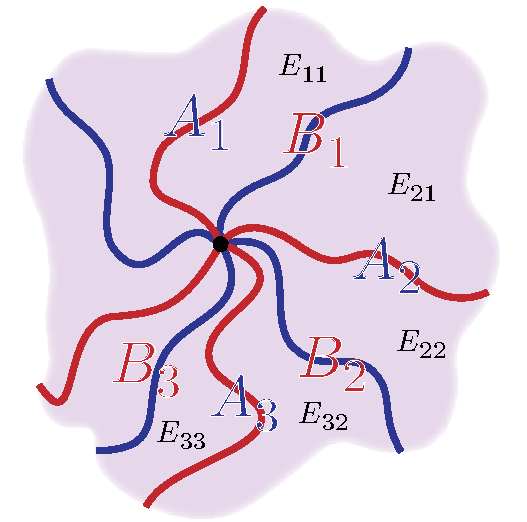
\includegraphics[trim=0cm 0cm 0cm 0cm, clip, scale=0.75]{images/additivita}
\end{center}
	Questo significa che $s(x)+t(x)=s_i+t_j,\ \forall x\in E_{ij}$, ossia
	\begin{equation*}
		s+t=\sum_{i,j}\left(s_i+t_j\right)\chi_{E_{ij}}
	\end{equation*}
	Integriamo secondo Lebesgue:
	\begin{equation*}
		\int_X\left(s+t\right)d\mu=\sum_{i,j}\left(s_i+t_j\right)\mu\left(E_{ij}\right)=\sum_{i,j}s_i\mu\left(E_{ij}\right)+\sum_{i,j}t_j\mu\left(E_{ij}\right)=\int_Xsd\mu+\int_Xtd\mu
	\end{equation*}
	\item \textbf{\textsc{Passo 2}:} proviamo il risultato nel caso di funzioni $\funz{f_1,f_2}{X}{\left[0,+\infty\right)}$ misurabili.\\
	È noto che:
	\begin{itemize}
		\item Esiste una successione di funzioni semplici misurabili $\funz{s_n}{X}{\left[0,+\infty\right]}$ tali che
		\begin{itemize}
			\item $0\leq s_n(x)\leq s_{n+1}(x)\leq f_1(x),\ \forall x\in X$.
			\item $\displaystyle \lim_{n\to+\infty}s_n(x)=f_1(x),\ \forall x\in\ X$
		\end{itemize}
		\item Esiste una successione di funzioni semplici misurabili $\funz{t_n}{X}{\left[0,+\infty\right]}$ tali che
		\begin{itemize}
			\item $0\leq t_n(x)\leq t_{n+1}(x)\leq f_2(x),\ \forall x\in X$.
			\item $\displaystyle \lim_{n\to+\infty}t_n(x)=f_2(x),\ \forall x\in\ X$
		\end{itemize}
	\end{itemize}
	Di conseguenza si ha
	\begin{align*}
		0\leq \left(s_n+t_n\right)(x)\leq \left(s_{n+1}+t_{n+1}\right)(x)\leq\left(f_1+f_2\right)(x),\ \forall x\in\ X\\
		\lim_{n\to+\infty}\left(s_n+t_n\right)(x)=\left(f_1+f_2\right)(x),\ \forall x\in\ X
	\end{align*}
	Integriamo secondo Lebesgue:
	\begin{align*}
		\int_X \left(f_1+f_2\right)d\mu&=\lim_{n\to+\infty}\int_X\left(s_n+t_n\right)d\mu&\text{(thm. conv. monotona)}\\
		&=\lim_{n\to+\infty}\left(\int_Xs_nd\mu+\int_Xt_nd\mu\right)&\text{(passo 1)}\\
		&=\lim_{n\to+\infty}\int_Xs_nd\mu+\lim_{n\to+\infty}\int_Xt_nd\mu&\\
		&=\int_Xf_1d\mu+\int_Xf_2d\mu&\text{(thm. conv. monotona)\qedhere}
	\end{align*}
	\end{itemize}
\end{demonstration}
Una conseguenza immediata di questa proprietà è che per le successioni di funzioni misurabili non negative vale lo \textit{scambio tra integrale e serie}.
\begin{corollary}[Scambio tra integrale e serie per funzioni misurabili e non negative]
Sia $\left(X,\mathcal{M},\mu\right)$ uno spazio di misura siano $\funz{f_n}{X}{\left[0,+\infty\right]},\ n\geq 1$ funzioni misurabili. Allora vale lo scambio tra integrale e serie:\index{scambio tra integrale e serie}
	\begin{equation}
		\int_X\left(\sum_{n=1}^{+\infty}f_n\right)d\mu=\sum_{n=1}^{+\infty}\int_Xf_nd\mu
	\end{equation}
\end{corollary}
\begin{demonstration}
	Consideriamo la successione delle ridotte
	\begin{equation*}
		g_k(x)=\sum_{n=1}^{k}f_n(x),\ \forall x\in X.
	\end{equation*}
	Ricordiamo che $g_k(x)$ è una successione crescente su $k$ per ogni $x\in X$, in quando $f_n(x)\geq 0$; poiché valgono le ipotesi del \textit{teorema della convergenza monotona} sulla successione $g_k$, possiamo applicarlo.\\
	Prima di farlo, osserviamo che per additività dell'integrale vale
	\begin{equation*}
		\int_X \sum_{n=1}^{k}f_n=\sum_{n=1}^{k}\int_X f_n
	\end{equation*}
	Noto ciò, dimostriamo facilmente il risultato desiderato: 
	\begin{align*}
		&\int \left(\lim_{k\to+\infty}g_k\right)d\mu=\lim_{k\to+\infty}\int_X g_kd\mu\\
		&\implies \int \left(\lim_{k\to+\infty}\sum_{n=1}^{k}f_n\right)d\mu=\lim_{k\to+\infty}\int_X \sum_{n=1}^{k}f_nd\mu=\lim_{k\to+\infty}\sum_{n=1}^{k}\int_X f_n\\
		&\implies \int_X\left(\sum_{n=1}^{+\infty}f_n\right)d\mu=\sum_{n=1}^{+\infty}\int_Xf_nd\mu\qedhere
	\end{align*}
\end{demonstration}
\subsection{Integrazione rispetto alla misura conteggio pesata}
\begin{theorema}[Integrazione rispetto alla misura conteggio pesata]\label{integrazionemisuraconteggiopesata}
	Sia $\left(\naturalset,\setpart{\naturalset},\mu_p\right)$ spazio di misura dove $\mu_p$ è la \textit{misura conteggio pesata} definita da
	\begin{align*}
		\mu_p\left(\left\{n\right\}\right)=p_n,\ \forall n\geq 1\text{ con }p_n\geq 0\\
		\mu_p\left(E\right)=\sum_{n\geq E}\mu_p\left(\left\{n\right\}\right),\ \forall E\subseteq \naturalset
	\end{align*}
Sia $\funz{f}{\naturalset}{\left[0,+\infty\right]}$. Allora si ha
\begin{equation*}
	\int_{\naturalset}fd\mu_p=\sum_{n\geq 1}f_np_n
\end{equation*}
In particolare, se $p_n=1,\ \forall n\geq 1$, si ha, indicata con $\mu^{\ast}$ la misura conteggio corrispondente,
\begin{equation*}
	\int_{\naturalset}fd\mu^{\ast}=\sum_{n\geq 1}f_n
\end{equation*}
\end{theorema}
\begin{observe}
	Nell'enunciato non è richiesta esplicitamente la misurabilità di $f$ in quanto ogni $\funz{f}{\left(\naturalset,\setpart{\naturalset}\right)}{\left[0,+\infty\right]}$ è \textit{sempre misurabile}. Infatti, $\forall A\subseteq \left[0,+\infty\right]$ aperto, la controimmagine $f^{-1}\left(A\right)$ è un sottoinsieme di $\naturalset$ e quindi $f^{-1}\left(A\right)\in \setpart{\naturalset}$.
\end{observe}
\begin{demonstration}
	Osserviamo che $f$ è una successione
	\begin{equation*}
		\left\{f_n\right\}_{n\geq 1}=\left\{f_1,\ f_2,\ f_3,\ \ldots\right\}
	\end{equation*}
Per $k\geq 1$ definiamo $\funz{g^k}{\naturalset}{\left[0,+\infty\right]}$ mediante
\begin{equation*}
	g^k_n=g^k\left(n\right)=\begin{cases}
		\begin{array}{ll}
			f_n &\text{se }n\leq k\\
			0 &\text{se }n>k
		\end{array}
	\end{cases}
\end{equation*}
Ad esempio:
\begin{gather*}
	\left\{g^1_n\right\}_{n\geq 1}=\left\{f_1,0,0,\ldots\right\}\\
	\left\{g^2_n\right\}_{n\geq 1}=\left\{f_1,f_2,0,\ldots\right\}\\
	\vdots\\
	\left\{g^k_n\right\}_{n\geq 1}=\left\{f_1,f_2,\ldots,f_k,0\ldots\right\}\\
\end{gather*}
Si ha $\displaystyle\lim_{k\to+\infty}g^k\left(n\right)=f_n=f\left(n\right),\ \forall n\geq 1$, quindi $g^k$ converge puntualmente a $f$ in ogni $n\in\naturalset$. Inoltre, $\forall n\in\naturalset$, la successione $g^k_n$ soddisfa
\begin{equation*}
	g^{k+1}_n\geq g^k_n,\ \forall k\geq 1
\end{equation*}
Pertanto, $g^k$ è una successione che converge \textit{puntualmente} in modo \textit{monotona crescente} a $f$. Per il \textit{teorema della convergenza monotona}, si ha
\begin{equation*}
	\int_{\naturalset}fd\mu_p=\lim_{k\to+\infty}\int_{\naturalset}g^kd\mu_p
\end{equation*}
Per ogni $k\in\naturalset$ calcoliamo $\displaystyle\int_{\naturalset}g^kd\mu_p$. Osserviamo che $g^k\left(\naturalset\right)=\left\{f_1,\ldots,f_k,0\right\}$, quindi $g^k$ è \textit{semplice} avendo immagine finita. Allora
\begin{equation*}
	\left(g^k\right)^{-1}\left(\left\{f_n\right\}\right)=n,\ \forall n\in\naturalset,\ n\geq k\\
	\left(g^k\right)^{-1}\left(\left\{0\right\}\right)=\left\{k+1,k+2,\ldots\right\}=A_0
\end{equation*}
Calcoliamo l'integrale:
\begin{equation*}
	\int_{\naturalset}d^kd\mu_p=\sum_{n=1}^{k}f_n\mu_p\left(\left\{n\right\}\right)+0\cdot \underbrace{\mu_p\left(A_0\right)}_{\substack{=0\ (\text{anche} \\ \text{nel caso } \\ 0\cdot \infty)}}=\sum_{n=1}^{k}f_np_n
\end{equation*}
Concludendo:
\begin{equation*}
	\int_{\naturalset}fd\mu_p=\lim_{k\to+\infty}\int_{\naturalset}g^kd\mu_p=\lim_{k\to+\infty}\sum_{n=1}^{k}f_np_n=\sum_{n=1}^{+\infty}f_np_n\qedhere
\end{equation*}
\end{demonstration}
Il seguente risultato, che abbiamo già incontrato\footnote{Si veda pag. \pageref{commutativitàindici}.} e che ci è servito per dimostrare la $\sigma$-additività dell'integrale di funzioni semplici rispetto al dominio, si può anche vedere come corollario dell'\textit{integrazione della misura conteggio semplice}, oltre che in modo \textit{elementare}. 
\begin{corollaryqed}[Commutatività degli indici nelle serie doppie]
	Se $a_{ij}\geq0\ \forall i,j$, allora
	\begin{equation*}
		\sum_{i=1}^{+\infty}\sum_{j=1}^{+\infty}a_{ij}=\sum_{j=1}^{+\infty}\sum_{i=1}^{+\infty}a_{ij}\qedhere
	\end{equation*}
\end{corollaryqed}
\subsection{Lemma di Fatou}
\begin{lemming}[Lemma di Fatou]\index{lemma!di Fatou}
	Se $\funz{f_n}{X}{\left[0,+\infty\right]}$ sono misurabili, $\forall n$, allora
	\begin{equation}
		\int_X\left(\liminf_{n\to+\infty}f_nd\mu\right)d\mu\leq \liminf_{n\to+\infty}\int_Xf_nd\mu
	\end{equation}
\end{lemming}
\begin{demonstration}
	Posto $\displaystyle g_k(x)\coloneqq\inf_{i\geq k}f_i(x)$ dove $k\geq 1,\ x\in X$, allora $g_k\leq f_k$ implica, per monotonia dell'integrale rispetto alle integrande,
	\begin{equation*}
		\circled[red]{\vardiamond}\quad\int_Xg_kd\mu\leq \int_Xf_kd\mu\implies \liminf_{k\to+\infty}\int_Xg_kd\mu\leq \liminf_{k\to+\infty}\int_Xf_kd\mu
	\end{equation*}
Osserviamo che:
\begin{itemize}
	\item $0\leq g_k(x)\leq g_{k+1}(x),\ \forall x\in X$ perché
	\begin{equation*}
		f_i(x)_{i\geq k}\supseteq f_i(x)_{i\geq k+1}\implies g_k(x)=\inf_{i\geq k}f_i(x)\leq\inf_{i\geq k+1}f_i(x)=g_{k+1}(x)
	\end{equation*}
	\item $g_k$ è misurabile, $\forall k\geq 1$ in quanto $\inf$ di funzioni misurabili.
\end{itemize}
Pertanto
	\begin{align*}
	\lim_{n\to+\infty}g_k(x)&=\sup_{k\geq i}\inf_{i\geq k}f_i(x)&\text{(teorema sul limite di successioni monotone)}\\
	&=\liminf_{n\to+\infty}f_n(x)&\text{(caratterizzazione del $\liminf$)}
\end{align*}
Per il \textit{teorema della convergenza monotona} si ha
\begin{equation*}
	\circled[blue]{\spadesuit}\quad \liminf_{k\to+\infty}\int_Xg_kd\mu=\lim_{k\to+\infty}\int_Xg_kd\mu=\int_X\lim_{n\to+\infty}g_kd\mu=\int_X\liminf_{k\to+\infty}f_kd\mu
\end{equation*}
Combinando $\circled[red]{\vardiamond}\ $ e $\ \circled[blue]{\spadesuit}\ $ otteniamo la tesi.
\end{demonstration}
\begin{observe}~{}
	\begin{itemize}
		\item Poiché $f_n$ sono misurabili e non negative, anche $\liminf_{n\to+\infty}$ è misurabile e non negativo e pertanto il suo integrale secondo Lebesgue esiste sempre. 
		\item Ci sono casi in cui vale \textit{soltanto} la disuguaglianza stretta.
	\end{itemize}
\end{observe}
\begin{examplewt}[Lemma di Fatou con disuguaglianza stretta]
	Sia $\left(X,\mathcal{M},\mu\right)=\left(\realset,\mathcal{L}(\realset),m_1\right)$ e $f_n(x)=\frac{1}{n}\chi_{\left[0,n\right]},\ \forall x\in\realset$.	Si ha
	\begin{equation*}
		\liminf_{n\to+\infty}f_n(x)=\lim_{n\to+\infty}f_n(x)=0\\
		\implies\int_{\realset}\left(\liminf_{n\to+\infty}f_n\right)dm_1=0
	\end{equation*}
	Mentre invece
	\begin{equation*}
		\liminf_{n\to+\infty}\int_{\realset}f_ndm_1=\liminf_{n\to+\infty}1=1
	\end{equation*}
\end{examplewt}
\subsection{{$\sigma$}-additività dell'integrale di funzioni misurabili non negative rispetto al dominio}
\begin{proposition}[{$\sigma$}-additività dell'integrale rispetto al dominio]
Sia $\left(X,\mathcal{M},\mu\right)$ uno spazio di misura e sia $\funz{f}{X}{\left[0,+\infty\right]}$ funzione misurabile.
Allora
\begin{equation}
	\int_{\bigcup_{n\geq 1}E_n}fd\mu=\sum_{n\geq 1}\int_{E_n}fd\mu,\ \forall E_n\in \mathcal{M}\colon E_i\cap E_j=\emptyset,\ \forall i\neq j
\end{equation}
\end{proposition}
\begin{demonstration}
	Posto $\displaystyle E\coloneqq \bigcup_{n\geq 1}E_n$, ricordiamo che
	\begin{equation*}
		\int_Efd\mu=\int_X\left(f\chi_E\right)d\mu\text{ con }f\chi_E=\begin{cases}
			\begin{array}{ll}
				f&\text{su }E\\
				0&\text{su }X\setminus E
			\end{array}
		\end{cases}
	\end{equation*}
Osserviamo che $\displaystyle \chi_E=\sum_{n\geq 1}\chi_{E_n}$ perché $\displaystyle E=\bigcup_{n\geq 1}E_n$ e $ E_i\cap E_j=\emptyset,\ \forall i\neq j$, pertanto
\begin{align*}
	\int_Efd\mu&=\int_X\left(f\chi_E\right)d\mu\\
	&=\int_X\left(f\sum_{n\geq 1}f\chi_{E_n}d\mu\right)=\int_X\sum_{n\geq 1}\underbrace{\left(f\chi_{E_n}\right)}_{\geq 0}d\mu\\
	&=\sum_{n\geq 1}\int_Xf\chi_{E_n}d\mu&\text{(scambio tra serie e integrale)}\\
	&=\sum_{g\geq 1}\int_{E_n}fd\mu&\qedhere
\end{align*}
\end{demonstration}
\begin{observe}
	Questo è il caso generale per \textit{funzioni misurabili} di un risultato precedentemente dimostrato per \textit{funzioni semplici}, misurabili, non negative. Notiamo che questo risultato richiede \textit{implicitamente} tale caso: infatti, nella dimostrazione abbiamo fatto uso del \textit{teorema della convergenza monotona}, che richiede la $\sigma$-additività rispetto al dominio delle funzioni semplici.
\end{observe}
\subsection{Misura indotta dall'integrale di Lebesgue}\label{misuraindotta}
Una conseguenza della $\sigma$-additività rispetto al dominio dell'integrale di Lebesgue è che, in modo analogo a come abbiamo visto per le funzioni semplici, possiamo costruire un \textit{nuovo spazio di misura} $\left(X,\mathcal{M},\mu_f\right)$ a partire da uno spazio di misura $\left(X,\mathcal{M},\mu\right)$ dato e una funzione $\funz{f}{X}{\left[0,+\infty\right]}$ misurabile.
\begin{corollaryqed}[Misura indotta dalla funzione misurabile non negativa]
Sia $\left(X,\mathcal{M},\mu\right)$ uno spazio di misura e sia $\funz{f}{X}{\left[0,+\infty\right]}$ misurabile. Allora la funzione
\begin{equation}
	\funztot{\mu_f}{\mathcal{M}}{\left[0,+\infty\right]}{E}{\int_Efd\mu}
\end{equation}
è una misura su $\mathcal{M}$.
\end{corollaryqed}
\begin{example}\label{gaussiana}
	Consideriamo $\left(\realset,\mathcal{L}(\realset),m_1\right)$ e prendiamo la \textbf{funzione gaussiana}\index{funzione!gaussiana}:
	\begin{equation*}
		f(x)=\frac{1}{\sqrt{2\pi}}e^{-\frac{x^2}{2}},\ \forall x\in\realset
	\end{equation*}
	La funzione è continua e dunque misurabile. La misura $\mu_f$ indotta è di probabilità dato che $\mu_f(\realset)=1$ e viene chiamata \textbf{misura di probabilità normale}\index{misura!di probabilità!normale}:
	\begin{gather*}
		\mu_f\left(E\right)=\int_E\frac{1}{\sqrt{2\pi}}e^{-\frac{x^2}{2}}dm_1,\ \forall E\in\mathcal{L}(\realset)\\
		\mu_f(\realset)=\int_{\realset}\frac{1}{\sqrt{2\pi}}e^{-\frac{x^2}{2}}dm_1=1
	\end{gather*}
\end{example}
Se consideriamo lo spazio di misura $\left(\realset,\mathcal{L}(\realset),\mu_f\right)$ e una funzione $\funz{g}{\realset}{\left[0,+\infty\right]}$ misurabile, possiamo definire \begin{equation*}
	\int_Egd\mu_f,\ \forall E\in\mathcal{L}(\realset)
\end{equation*}
Cos'è questo integrale? La risposta tale quesito è il seguente teorema.
\begin{theorema}[Integrale rispetto alla misura indotta]
	Dato $\left(X,\mathcal{M},\mu\right)$ uno spazio di misura e $\funz{f}{X}{\left[0,+\infty\right]}$ misurabile, consideriamo lo spazio di misura indotto $\left(X,\mathcal{M},\mu_f\right)$ con
	\begin{equation*}
		\funztot{\mu_f}{\mathcal{M}}{\left[0,+\infty\right]}{E}{\int_Efd\mu}
	\end{equation*}
	Sia $\funz{g}{X}{\left[0,+\infty\right]}$ misurabile. Allora
	\begin{equation}
		\int_Xgd\mu_f=\int_Xgfd\mu
	\end{equation}
\end{theorema}
\begin{demonstration}
	Innanzitutto, prima dimostriamo la proprietà per funzioni caratteristiche, poi per combinazioni lineari di esse (funzioni semplici), poi consideriamo il caso di una funzione $f$ misurabile non negativa, approssimandola co una successione di funzioni semplici misurabili.\\
	\begin{enumerate}[label=\Roman*]
		\item Sia $g=\chi_A$ con $A\in\mathcal{M}$ (pertanto $g$ è misurabile). Si ha
		\begin{equation*}
			\int_X\chi_Ad\mu_f=\int_A 1d\mu_f=1\mu_f\left(A\right)=\mu_f\left(A\right)\underset{\substack{\text{def.}\\\text{ di }\mu_f}}{=}\int_Afd\mu=\int_X\left(\chi_Afd\mu\right)
		\end{equation*}
		\item Sia $\funz{g}{X}{\left[0,+\infty\right)}$ misurabile semplice, scritta nella decomposizione standard come
		\begin{equation*}
			g=\sum_{i=1}^kg_i\chi_{A_i}\quad\text{con }g(X)=\left\{g_1,\ldots,g_k\right\}\text{ e }A_i=g^{-1}\left(\left\{g_i\right\}\right),\ i=1,\ \ldots,\ k
		\end{equation*}
	Allora
	\begin{align*}
			\int_Xgd\mu_f&=\int_X\left(\sum_{i=1}^kg_i\chi_A\right)d\mu_f)\sum_{i=1}^{k}g_i\int_X\chi_{A_i}d\mu_f\underset{\text{passo }1}{=}\sum_{i=1}^{k}g_i\int_X\chi_Afd\mu=\\
			&=\int_X\underbrace{\sum_{i=1}^{k}g_i\chi_{A_i}}_{=g}fd\mu=\int_Xgfd\mu
	\end{align*}
	\item Consideriamo $\funz{g}{X}{\left[0,+\infty\right]}$ misurabile. È noto che esiste una successione $\funz{g_n}{X}{\left[0,+\infty\right)}$ di funzioni semplici misurabili tali
	\begin{itemize}
		\item $\displaystyle\lim_{n\to+\infty}g_n(x)=g(x),\ \forall x\in X$.
		\item $g_{n+1}(x)\leq g_n(x),\ \forall x\in\ X,\ \forall n\geq 1$.
	\end{itemize}
Allora
	\begin{equation*}
	\int_Xgd\mu_f\underset{\substack{\text{thm. di}\\\text{convergenza}\\\text{monotona}}}{=}\lim_{n\to+\infty}\int_Xg_nd\mu_f\underset{\text{passo }2}{=}\lim_{n\to+\infty}\int_Xg_nfd\mu
	\end{equation*}
Osservando che
\begin{itemize}
	\item $\displaystyle\lim_{n\to+\infty}\left(g_nf\right)(x)=\left(gf\right)(x),\ \forall x\in X$.
	\item $\left(g_{n+1}f\right)(x)\leq \left(g_nf\right)(x),\ \forall x\in\ X,\ \forall n\geq 1$.
\end{itemize}
possiamo concludere, per il \textit{teorema di convergenza monotona}, che
\begin{equation*}
	\int_Xgd\mu_f=\int_X\left(gf\right)d\mu\qedhere
\end{equation*}
	\end{enumerate}
\end{demonstration}
\begin{example}
	Riprendiamo l'esempio visto in precedenza\footnote{Si veda pag. \pageref{gaussiana}.} della funzione gaussiana
	\begin{equation*}
		f(x)=\frac{1}{\sqrt{2\pi}}e^{-\frac{x^2}{2}},\ \forall x\in X
	\end{equation*}
	In $\left(\realset,\mathcal{L}(\realset),m_1\right)$ essa implica la misura di probabilità ($\mu_f(X)=1$) normale
	\begin{equation*}
		\mu_f\left(E\right)=\int_E\frac{1}{\sqrt{2\pi}}e^{-\frac{x^2}{2}},\ \forall E\in \mathcal{L}(\realset)
	\end{equation*}
la quale induce il nuovo spazio di misura $\left(\realset,\mathcal{L}(\realset),\mu_f\right)$. Se $\funz{g}{\realset}{\left[0,+\infty\right]}$ misurabile, allora
\begin{equation*}
	\int_\realset gd\mu_f=\int_\realset\frac{1}{\sqrt{2\pi}}g(x)e^{-\frac{x^2}{2}}dm_1
\end{equation*}
Osserviamo che per $g(x)=x^k$ quello che otteniamo integrando rispetto alla misura $\mu_f$ è il momento $k$-esimo di $f$.
\end{example}
\subsection{Misure assolutamente continue}
Ricordiamo che se $\funz{f}{X}{\left[0,+\infty\right]}$ è misurabile, allora
\begin{equation*}
		\mu_f\left(E\right)=\int_Efd\mu=0,\ \forall E\in\mathcal{M}\colon \mu\left(E\right)=0
\end{equation*}
Riscriviamo questa relazione come
\begin{equation*}
	\forall E\in\mathcal{M}\colon\mu\left(E\right)=0\implies \mu_f\left(E\right)=0
\end{equation*}
Questo si esprime dicendo che $\mu_f$ è \textbf{assolutamente continua rispetto a} $\mu$ e si indica $\mu_f \ll \mu$.
\begin{define}[Continuità assoluta per una misura]
	Sia $\left(X,\mathcal{M},\mu\right)$ uno spazio di misura e sia $\funz{\lambda}{X}{\left[0,+\infty\right]}$. $\lambda$ si dice \textbf{assolutamente continua rispetto a }$\mu$\index{continuità assoluta} se
	\begin{equation}
		\forall E\in\mathcal{M}\colon \mu\left(E\right)=0\implies \lambda\left(E\right)=0
	\end{equation}
e si indica come $\lambda \ll \mu$.
\end{define}
\begin{examples}~{}
	\begin{itemize}
		\item \textsc{\textbf{Misura assolutamente continua.}}\\
		Se $\funz{f}{X}{\left[0,+\infty\right]}$ misurabile, $\mu_f$ definita precedentemente è assolutamente continua rispetto a $\mu$
		\item \textsc{\textbf{Misura non assolutamente continua.}}\\
		Sia $\left(\realset,\mathcal{L}(\realset),m_1\right)$ e consideriamo la \textit{misura conteggio}
		\begin{equation*}
			\funztot{\lambda}{\mathcal{L}(\realset)}{\left[0,+\infty\right]}{E}{\begin{cases}
					\begin{array}{ll}
						\# E&\text{se }E\text{ è finito}\\
						+\infty&\text{se }E\text{ è infinito}
					\end{array}
			\end{cases}}
		\end{equation*}
		$\lambda$ \textit{non} è assolutamente continua rispetto a $m_1$: infatti, preso $E=\left\{\overline{x}\right\}$, con $\overline{x}\in\realset$, si ha
		\begin{equation*}
			m_1\left(\left\{\overline{x}\right\}\right)=0\text{ ma }\lambda\left(\left\{\overline{x}\right\}\right)=1
		\end{equation*}
	\end{itemize}
\end{examples}
Diamo ora una caratterizzazione delle misure assolutamente continue finite.
\begin{theoremaqed}[Caratterizzazione delle misure ass. cont. finite]
Sia $\left(X,\mathcal{M},\mu\right)$ uno spazio di misura e sia $\funz{\lambda}{\mathcal{M}}{\left[0,+\infty\right)}$ una misura \textit{finita}, ossia tale per cui $\lambda(X)<+\infty$.
Allora
\begin{equation}
	\lambda\ll\mu\iff\forall \epsilon>0,\ \exists\delta>0\colon\forall E\in\mathcal{M}\colon \mu\left(E\right)<\delta\implies \lambda\left(E\right)<\epsilon\qedhere
\end{equation}
\end{theoremaqed}
Tra le misure assolutamente rispetto ad una misura $\mu$ ci sono le misure del tipo $\mu_f$ introdotte prima. Ci si potrebbe chiedere se ce ne sono altre: se $\mu$ è $\sigma$-finita, ossia se soddisfa
\begin{equation*}
	\mu(X)=+\infty\quad X=\bigcup_{n\geq 1}X_n,\ \mu\left(X_n\right)<+\infty
\end{equation*}
La risposta è \textbf{no}, come si può vedere dal teorema seguente.
\begin{theoremaqed}[Teorema di Radon-Nikodym]\index{teorema!di Radon-Nikodym}
	Sia $\left(X,\mathcal{M},\mu\right)$ uno spazio di misura con $\mu$ misura $\sigma$-finita e sia $\funz{\lambda}{X}{\left[0,+\infty\right]}$ una misura. Allora
	\begin{equation}
		\lambda\ll\mu\iff \exists \funz{f}{X}{\left[0,+\infty\right]}\colon\lambda\left(E\right)=\int_Efd\mu,\ \forall E\in\mathcal{M}
	\end{equation}
La funzione $f$ viene detta \textbf{derivata di Radon-Nikodym} o \textbf{densità}\index{densità}.
\end{theoremaqed}
\section{Integrabilità}
Ci stiamo avvicinando al terzo e ultimo passo dell'integrale di Lebesgue: lo scopo è quello di estendere la definizione per funzione \textit{a valori complessi}.\\
Tuttavia, a differenza del passo 2, dove l'integrale può essere assumere valori in $\left[0,+\infty\right]$, l'insieme dei complessi $\complexset$ non contempla il valore $+\infty$; inoltre, come vedremo, la costruzione dell'integrale scelta può presentare delle \textit{forme di indecisione} che \textit{non} possiamo risolvere.\\
Per proseguire, dobbiamo necessariamente considerare una classe particolare di funzioni misurabili, le \textbf{funzioni integrabili}\index{funzione!integrabile}\seeonlyindex{integrabilità}{funzione!integrabile}.
\begin{define}[Integrabilità]
	Sia $\left(X,\mathcal{M},\mu\right)$ uno spazio di misura e sia $\funz{f}{X}{\complexset}$. La funzione $f$ si dice \textbf{integrabile} se
	\begin{enumerate}
		\item $f$ misurabile.
		\item $\displaystyle\int_X\abs{f}d\mu<+\infty$ dove $\funz{\lvert f\rvert}{X}{\left[0,+\infty\right]}$
	\end{enumerate}
Indichiamo l'insieme delle funzioni integrabili come $\mathcal{L}^{1}\left(\mu\right)$.
\end{define}
\begin{observe}
		Per definizione $f\in\mathcal{L}^{1}\left(\mu\right)\iff\abs{f}\in\mathcal{L}^{1}\left(\mu\right)$.
\end{observe}
\begin{attention}
	 Nel caso particolare $\funz{f}{X}{\left[0,+\infty\right)}$, se $f$ è misurabile allora esiste
	\begin{equation*}
		\int_Xfd\mu
	\end{equation*}
	finito o $+\infty$, dunque $\funz{f}{X}{\left[0,+\infty\right)}$ misurabile ammette \textit{sempre} integrale secondo Lebesgue, ma è integrabile solo se 
	\begin{equation*}
		\int_Xfd\mu<+\infty
	\end{equation*}
\end{attention}
\begin{proposition}[Le funzioni integrabili formano uno spazio vettoriale]
	$\mathcal{L}^1\left(\mu\right)$ è uno spazio vettoriale con le operazioni di somma di funzioni e prodotto di una funzione per uno scalare.
\end{proposition}
\begin{demonstration}
	Siano $f,g\in\mathcal{L}^{1}\left(\mu\right),\ \alpha,\beta\in\complexset$. Allora:
	\begin{enumerate}
		\item $\alpha f+\beta g$ misurabile perché $f$ e $g$ sono misurabili.
		\item
		\begin{equation*}
			\int_X\abs{\alpha f+\beta g}d\mu\leq \int_X\abs{\alpha}\abs{f}+\abs{\beta}\abs{g}d\mu=\abs{\alpha}\underbrace{\int_X\abs{f}d\mu}_{\substack{<+\infty\\\text{perché }\\f\text{ int.}}}+\underbrace{\abs{\beta}\int_X\abs{g}d\mu}_{\substack{<+\infty\\\text{perché }\\g\text{ int.}}}<+\infty
		\end{equation*}
	\end{enumerate}
Pertanto $\alpha f+\beta g\in\mathcal{L}^{1}\left(\mu\right)$.
\end{demonstration}
\subsection{Decomposizione di una funzione a valori complessi in termini di funzioni a valori reali non negativi}
Come fu utilizzato il passo 1 dell'integrale di Lebesgue per definire il passo 2, ci interessa utilizzare il secondo passo dell'integrale di Lebesgue per definire il terzo. Lo scopo quindi è di scomporre una generica funzione $\funz{f}{X}{\complexset}$ integrabile in una combinazione lineare di funzioni non negative ancora integrabili, in modo che il loro integrale sia definito. Per far ciò, consideriamo la \textit{parte reale} e \textit{immaginaria} di $f$:\\
\begin{tabular}{ l l }
	\quad{\scriptsize $\blacksquare $}\ \textbf{Parte reale:} & $\funz{u\coloneqq \Re f}{X}{\realset}$ \\
	\quad{\scriptsize $\blacksquare $}\ \textbf{Parte immaginaria:} & $\funz{v\coloneqq \Im f}{X}{\realset}$  
\end{tabular}\\
In questo modo, abbiamo scomposto $f$ come una combinazione lineare di funzioni misurabili reali, ma possono assumere valori anche negativi. Decomponiamo ulteriormente $u$ e $v$ usando le \textit{parti positive} e \textit{parti negative}:\\
\begin{tabular}{ l l }
	\quad{\scriptsize $\blacksquare $}\ \textbf{Parte positiva di} $u$: & $u^{+}\coloneqq \max\left(u,0\right)\geq 0$ \\
	\quad{\scriptsize $\blacksquare $}\ \textbf{Parte negativa di} $u$: & $u^{-}\coloneqq \max\left(-u,0\right)\geq 0$ \\
	\quad{\scriptsize $\blacksquare $}\ \textbf{Parte positiva di} $v$: & $v^{+}\coloneqq \max\left(v,0\right)\geq 0$ \\
	\quad{\scriptsize $\blacksquare $}\ \textbf{Parte negativa di} $v$: & $v^{-}\coloneqq \max\left(-v,0\right)\geq 0$ \\
\end{tabular}\\
Ottenendo così $u=u^{+}-u^{-}$ e $v=v^{+}-v^{-}$.
\vspace{4mm}\\
\begin{minipage}{0.5\textwidth}
	\begin{center}
		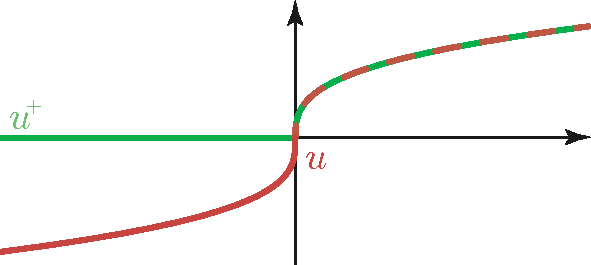
\includegraphics[trim=0cm 0cm 0cm 0cm, clip, scale=0.65]{images/partepositiva}
	\end{center}
\end{minipage}
\begin{minipage}{0.5\textwidth}
	\begin{center}
		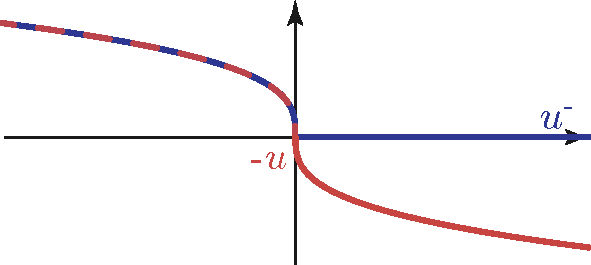
\includegraphics[trim=0cm 0cm 0cm 0cm, clip, scale=0.65]{images/partenegativa}
	\end{center}
\end{minipage}\vspace{4mm}\\
Tornando quindi a $\funz{f}{X}{\complexset}$, possiamo ottenere $f$ come combinazione lineare di quattro funzioni reali \textit{non negative}.
\begin{equation}
	f=\left(\Re f\right)+i\left(\Im f\right)=\left(\left(\Re f\right)^{+}-\left(\Re f\right)^{-}\right)+i\left(\left(\Im\right)^{+}-\left(\Im\right)^{-}\right)
\end{equation}
Con la prossima proposizione dimostreremo che le funzioni qui definite sono tutte integrabili.
\begin{proposition}[Integrabilità delle parti positive e negative delle parti reali e immaginarie]\label{integrabilitàpartiposnegrealimm}
	Se $f\in\mathcal{L}^{1}\left(\mu\right)$, allora $\left(\Re f\right)^{\pm},\ \left(\Im f\right)^{\pm}\in\mathcal{L}^{1}\left(\mu\right)$.
\end{proposition}
\begin{demonstration}
	Poiché $f\in\mathcal{L}^{1}\left(\mu\right)$, allora $\Re f$ e $\Im f$ sono misurabili; ne consegue che $\left(\Re f\right)^{\pm},\ \left(\Im f\right)^{\pm}\in\mathcal{L}^{1}\left(\mu\right)$ sono misurabili\footnote{Si vedano le ‘‘Note aggiuntive'', a pag. \pageref{misuraparterealeimm}.}, reali e non negative, dunque coincidono con il loro modulo.\\
	Poiché ogni funzione misurabile, reale, non negativa è integrabile, ciò implica che la seconda ipotesi per l'integrabilità è soddisfatta e quindi vale la tesi.
\end{demonstration}
\section{Passo 3: funzioni complesse integrabili}
Avendo enunciato tutte le premesse del caso, siamo nelle condizioni di enunciare il terzo passo dell'integrale di Lebesgue.
\begin{define}[Integrale di Lebesgue per funz. a valori complessi, integrabili]
	Sia $\funz{f}{\left(X,\mathcal{M},\mu\right)}{\complexset}$ funzione \textit{integrabile}. Posto
	\begin{equation*}
		f=\left(\Re f\right)^{+}-\left(\Re f\right)^-+i\left[\left(\Im f\right)^{+}-\left(\Im f\right)^{-}\right]
	\end{equation*}
si definisce l'\textit{integrale esteso ad E di $f$ rispetto alla misura $\mu$} come
\begin{equation}
	\int_Efd\mu\coloneqq\int_E\left(\Re f\right)^{+}d\mu-\int_E\left(\Re f\right)^{-}+i\left(\int_E\left(\Im f\right)^{+}d\mu-\int_E\left(\Im f\right)^{-}d\mu\right)
\end{equation}
\end{define}
\begin{observe}
	L'ipotesi $f\in\mathcal{L}^{1}\left(\mu\right)$ implica, come dice la proposizione \ref{integrabilitàpartiposnegrealimm}, che $\left(\Re f\right)^{\pm}$, $\left(\Im_f\right)^{\pm}\in\mathcal{L}^1\left(\mu\right)$ e quindi vale
	\begin{equation*}
		\int_X\left(\Re f\right)^{\pm}d\mu<+\infty\quad \int_X\left(\Im f\right)^{\pm}d\mu<+\infty
	\end{equation*}
	Di conseguenza, tale integrale esiste finito in $\complexset$. Se infatti le quattro funzioni ottenute decomponendo $f$ non fossero integrabili, allora potrebbero capitare delle situazioni in cui \textit{due degli integrali} della scomposizione danno la \textit{forma indeterminata} $\infty-\infty$.
\end{observe}
\begin{property}[Proprietà dell'integrale di Lebesgue per funzioni a valori in {$\complexset$}]
	Sia $\left(X,\mathcal{M},\mu\right)$ uno spazio di misura.
	\begin{enumerate}
		\item \textbf{Linearità:}
		\begin{equation}
			\int_X\left(\alpha f+\beta g\right)d\mu=\alpha\int_Xfd\mu+\beta\int_Xgd\mu,\ \forall f,g\in\mathcal{L}^1\left(\mu\right),\ \forall\alpha,\ \beta\in\complexset
		\end{equation}
		\item \textbf{Monotonia rispetto al modulo:}
		\begin{equation}
			\abs{\int_Xfd\mu}\leq \int_X\abs{f}d\mu,\ \forall f\in\mathcal{L}^1\left(\mu\right)
		\end{equation}
	\item $\sigma$-\textbf{additività rispetto al dominio:} se $\displaystyle E=\bigcup_{n\geq 1}E_n,\ \forall E_n\in\mathcal{M}\colon E_i\cap E_j=\emptyset,\ \forall i\neq j$, allora
	\begin{equation}
		f\in\mathcal{L}^1\left(\mu\right)\implies \int_Efd\mu=\sum_{n\geq 1}\int_{E_n}fd\mu
	\end{equation}
\item \textbf{Assoluta continuità:}
\begin{equation}
	f\in\mathcal{L}^{1}\left(\mu\right)\implies \forall \epsilon>0,\ \exists \delta >0\colon\forall E\in\mathcal{M}\colon \mu\left(E\right)<\delta\implies\abs{\int_E fd\mu}<\epsilon
\end{equation}
in altre parole, l'integrale si può rendere arbitrariamente più piccolo in modulo a patto di integrare su un dominio di misura sufficientemente piccola.
\end{enumerate}
\end{property}
\begin{demonstration}
	Dimostriamo l'assoluta continuità (punto 4).\\
	Consideriamo $\funz{f}{X}{\complexset}$ con $f\in\mathcal{L}^1\left(\mu\right)$; sappiamo che $f$ è misurabile e pertanto anche $\funz{\lvert f\rvert}{X}{\left[0,+\infty\right)}$ la è.\\
	Consideriamo la misura
	\begin{equation*}
		\funztot{\mu_{|f|}}{\mathcal{M}}{\left[0,+\infty\right]}{E}{\int_E\abs{f}d\mu}
	\end{equation*}
Essa è assolutamente continua rispetto a $\mu$. Inoltre, $\mu_{\abs{f}}$ è finita perché $f\in\mathcal{L}^1\left(\mu\right)$ e quindi
\begin{equation*}
	\mu_{\abs{f}}(X)=\int_X\abs{f}d\mu<+\infty
\end{equation*}
Per la caratterizzazione delle misure finite assolutamente continue rispetto a $\mu$ si ha
\begin{equation*}
	\forall \epsilon >0,\ \exists \delta > 0\colon E\in\mathcal{M},\ \mu\left(E\right)<\delta\implies \mu_{\abs{f}}\left(E\right)=\int_E\abs{f}d\mu<\epsilon
\end{equation*}
Si ha quindi
\begin{equation*}
	\forall \epsilon > 0,\ \exists \delta >0\colon \exists E\in\mathcal{M},\ \mu\left(E\right)<\delta\implies \abs{\int_Efd\mu}\underset{\substack{\text{prop. }2\\\text{dell'int.}}}{\leq}\int_E\abs{f}d\mu<\epsilon\implies \abs{\int_Efd\mu}<\epsilon\qedhere
\end{equation*}
\end{demonstration}
\subsection{Teorema della convergenza dominata}\index{teorema!della convergenza dominata}
\begin{theorema}[Teorema della convergenza dominata]\label{thmconvergenzadominata}
Siano $\left(X,\mathcal{M},\mu\right)$ uno spazio di misura e $\funz{f_n,f}{X}{\complexset}$ con $n\geq 1$ tali che
\begin{enumerate}[label=(\alph*)]
	\item 	$f_n$ sono misurabili.
	\item 	$\displaystyle \lim_{n\to+\infty}f_n(x)=f(x),\ \forall x\in X$
	\item 	Esiste una funzione $g\in \mathcal{L}^{1}\left(\mu\right)$ tale per cui
\begin{equation*}
	\abs{f_n(x)}\leq g(x),\ \forall n\geq 1,\ \forall x\in X
\end{equation*}
\end{enumerate}
Allora
\begin{enumerate}
	\item $f\in L^{1}\left(\mu\right)$.
	\item $\displaystyle\lim_{n\to+\infty}\int_X\abs{f_n-f}d\mu=0$
	\item Vale il \textbf{passaggio al limite sotto segno di integrale}\index{passaggio al limite sotto segno di integrale}:
	\begin{equation}
		\lim_{n\to+\infty}\int_Xf_nd\mu=\int_Xfd\mu
	\end{equation}
\end{enumerate}
\end{theorema}
\begin{demonstration}
	Poiché $f_n$ è una successione di funzioni misurabili che converge puntualmente a $f$, $\forall x\in X$, $f$ è una funzione misurabile. Inoltre, dato che tutti gli elementi della successione $f_n$ sono maggiorati (in modulo) da $g$, si ha per monotonia del limite che
	\begin{equation*}
		\circled[red]{\vardiamond}\quad \abs{f}\leq g
	\end{equation*}
	Allora, applicando i moduli ai membri della disequazione vale $\abs{f}\leq\abs{g}$. Integrando rispetto a Lebesgue, per monotonia rispetto all'integranda si ha
	\begin{equation*}
		\int_X\abs{f}d\mu\leq \int_X \abs{g}d\mu<+\infty
	\end{equation*}
	in quanto $g\in \mathcal{L}^1\left(\mu\right)$; segue che $f\in \mathcal{L}^1\left(\mu\right)$.\\
	Osserviamo che
	\begin{align*}
		\abs{f_n-f}&\leq \abs{f_n}+\abs{f}&\text{(disuguaglianza triangolare)}\\
		&\leq2g&\text{(per $\circled[red]{\vardiamond}$)}
	\end{align*}
	da cui segue che $2g-\abs{f_n-f}\geq 0$ e quindi sono funzioni non negative. Poiché le $2g-\abs{f_n-f}$ sono misurabili in quanto somma di funzioni in $\mathcal{L}^1\left(\mu\right)$ (e quindi misurabili), possiamo applicare il \textit{lemma di Fatou} a tali funzioni e ottenere
	\begin{gather*}
		\int_X\left(\liminf_{n\to+\infty}2g-\abs{f_n-f}\right)d\mu\leq\liminf_{n\to+\infty}\int_X\left(2g-\abs{f_n-f}\right)d\mu\\
		\viff\\
		\int_X 2gd\mu-\int_X\liminf_{n\to+\infty}\abs{f_n-f}d\mu\leq\int_X 2gd\mu+\liminf_{n\to+\infty}\left(-\int_X\abs{f_n-f}d\mu\right)
	\end{gather*}
	ma
	\begin{equation*}
		\int_X\liminf_{n\to+\infty}\abs{f_n-f}d\mu=0
	\end{equation*}
	in quanto per ipotesi $\displaystyle\lim_{n\to+\infty}f_n=f\iff\lim_{n\to+\infty}\abs{f_n-f}=0$; segue che $\liminf$ e $\lim$ coincidono con valore $0$ e pertanto anche l'integrale risulta nullo.\\
	Inoltre, notiamo che
	\begin{equation*}
		\int_X\abs{f_n-f}d\mu
	\end{equation*}
	è una successione a valori non negativi, dunque per le proprietà del massimo e minimo limite\footnote{Nell'approfondimento ‘‘Massimo e minimo limite'', a pag. \pageref{maxminlegame} è possibile trovare la dimostrazione di questo risultato insieme ad altri relativi al limsup e liminf.} si ha
	\begin{equation*}
		\liminf_{n\to+\infty}\left(-\int_X\abs{f_n-f}d\mu\right)=-\limsup_{n\to+\infty}\left(\int_X\abs{f_n-f}d\mu\right)
	\end{equation*}
	Allora otteniamo
	\begin{equation*}
		\int_X 2gd\mu\leq\int_X 2gd\mu-\limsup_{n\to+\infty}\left(\int_X\abs{f_n-f}d\mu\right)
	\end{equation*}
	Dato che $g\in \mathcal{L}^1\left(\mu\right)$ è non negativa, si ha  
	\begin{equation*}
		\int_X2gd\mu=2\int_X\abs{g}d\mu<+\infty
	\end{equation*}
	Possiamo dunque sottrarre
	\begin{equation*}
		\int_X 2gd\mu
	\end{equation*}
	da entrambi i membri della disequazione e ottenere
	\begin{equation*}
		\circled[blue]{\spadesuit}\quad \limsup_{n\to+\infty}\int_X\abs{f_n-f}d\mu\leq 0
	\end{equation*} 
	Notiamo che se una successione di numeri reali non negativi non converge a $0$, allora il massimo limite è positivo.\footnote{Infatti, se $a_n\geq 0,\ \forall n\in\naturalset$, allora anche il limite $\displaystyle \lim_{n\to+\infty}a_n$ sarà non negativo.  Tuttavia, poiché tale successione ammette limite, allora esso coincide con il suo massimo limite. Segue immediatamente che
	\begin{equation*}
		\lim_{n\to+\infty}a_n\neq0\implies \lim_{n\to+\infty}a_n>0\implies \limsup_{n\to+\infty}a_n>0
	\end{equation*}} Per contronominale, se il massimo limite di numeri reali non negativi \textit{non} è positivo, allora la serie converge a $0$ necessariamente. Poiché vale \circled[blue]{\spadesuit}, allora ciò implica la prima tesi:
	\begin{equation*}
		\lim_{n\to+\infty}\int_X\abs{f_n-f}d\mu=0
	\end{equation*}
	Infine, poiché l'integrale di Lebesgue è monotono rispetto al modulo, si ha
	\begin{equation*}
		0=\lim_{n\to+\infty}\int_X\abs{f_n-f}d\mu\geq\lim_{n\to+\infty}\abs{\int_X\left(f_n-f\right)d\mu}\ge 0
	\end{equation*}
	e quindi
	\begin{equation*}
		\lim_{n\to+\infty}\abs{\int_X \left(f_n-f\right)d\mu}=0\implies\lim_{n\to+\infty}\int_X\left(f_n-f\right)d\mu=0\implies\lim_{n\to+\infty}\int_X f_nd\mu=\int_X fd\mu
	\end{equation*}
	ottenendo la seconda e ultima tesi.
\end{demonstration}
\section{Tra integrale di Riemann e integrale di Lebesgue}
Nell'excursus storico abbiamo visto come l'\textit{integrale di Lebesgue} e le sue successive astrazioni di inizio '900 siano state la risposta a due domande che indirizzarono gli studi di Analisi del XIX secolo:
\begin{itemize}
	\item Come si può allargare la classe delle funzioni integrabili?
	\item Come si può caratterizzare l'insieme dei punti di discontinuità di una funzione integrabile secondo Riemann?
\end{itemize}
Con i tre passi precedentemente esposti abbiamo costruito l'integrale astratto di Lebesgue e risposto alla prima domanda, mentre rimane al momento aperta la seconda; in particolare, nel caso di funzioni da $\realset$ a $\realset$, sorge la questione: \textit{che relazione c'è tra l'integrale di Riemann e l'integrale di Lebesgue?}\\
Nel caso di funzioni limitate su un intervallo chiuso e che sono Riemann-integrabili scopriamo che tali integrali coincidono.
\begin{theoremaqed}[Integrale proprio di Riemann implica integrale di Lebesgue]
	Sia $\funz{f}{\left[a,b\right]}{\realset}$ limitata e misurabile. Allora
	\begin{equation}
		f\in\mathcal{R}\left(\left[a,b\right]\right)\implies f\in\mathcal{L}^1\left(\left[a,b\right],m_1\right)
	\end{equation}
e
\begin{equation}
	\int_{\left[a,b\right]}\abs{f}dm_1=\int_{a}^{b}f(x)dx\qedhere
\end{equation}
\end{theoremaqed}
% TO DO: add cenni dimostrazione
\begin{observes}~
	\begin{itemize}
		\item Il viceversa non è vero: come abbiamo già visto\footnote{Si veda pag. \pageref{funzionedirichletintegrale}.}, la funzione di Dirichlet è integrabile secondo Lebesgue ma non secondo Riemann.
		\item L'ipotesi di misurabilità è in realtà ridondante: come si potrà vedere con i risultati della sezione successiva, ogni funzione limitata e Riemann-integrabile è sempre misurabile rispetto alla misura di Lebesgue $m_1$.
	\end{itemize}
\end{observes}
Situazione differente si ha con l'integrale improprio di Riemann: infatti, può capitare che ci siano funzioni integrabili (almeno impropriamente) secondo Riemann ma \textit{non} secondo Lebesgue!
\begin{theoremaqed}[Integrale improprio di Riemann e integrale di Lebesgue]\label{integraleimproprioriemannlebesgue}
	Sia $\funz{f}{\left[a,+\infty\right]}{\realset}$ misurabile tale che $f\in\mathcal{R}\left(\left[a,b\right]\right)$ per ogni $b>a$. Allora
	\begin{enumerate}
		\item Vale la relazione
		\begin{equation}
			\int_{\left[a,+\infty\right)}\abs{f}dm_1=\int_{0}^{+\infty}\abs{f(x)}dx\in\left[0,+\infty\right]
		\end{equation}
		\item Se l'integrale improprio di Riemann di $f$ su $\left[a,+\infty\right)$ converge \textit{assolutamente} allora $f$ è integrabile secondo Lebesgue su $\left[a,+\infty\right)$ e
		\begin{equation}
			\int_{\left[a,+\infty\right)}fdm_1=\int_{a}^{+\infty}f(x)dx\in\realset\qedhere
		\end{equation}
	\end{enumerate}
\end{theoremaqed}
\begin{observe}
	CI sono risultati analoghi per gli integrali impropri di Riemann della forma
	\begin{align*}
		\int_{-\infty}^{b}f(x)dx&=\lim_{a\to-\infty}\int_{a}^{b}f(x)dx\\
		\int_{a}^{\gamma}f(x)dx&=\lim_{b\to \gamma^{-}}\int_{a}^{b}f(x)dx\\
		\int_{\gamma}^{b}f(x)dx&=\lim_{a\to \gamma^{+}}\int_{a}^{b}f(x)dx
	\end{align*}
\end{observe}
\begin{attention}
	Se l'integrale improprio di Riemann di $f$ su $\left[a,+\infty\right)$ converge ma non \textit{assolutamente} allora $f$ \textit{non} è integrabile secondo Lebesgue su $\left[a,+\infty\right)$.
\end{attention}
\begin{example}
	Consideriamo la funzione
	\begin{equation*}
		f(x)=\frac{\sin x}{x}
	\end{equation*}
	sull'intervallo $\left[\pi,+\infty\right)$. Mostriamo che:
	\begin{enumerate}
		\item L'integrale di $f$ secondo Riemann converge semplicemente.
		\item L'integrale di $f$ secondo Riemann \textit{non} converge assolutamente.
		\item La funzione $f$ \textit{non} è integrabile secondo Lebesgue.
	\end{enumerate}
\begin{enumerate}[label=\Roman*]
	\item Integrando per parti si ha
	\begin{align*}
		\int_{\pi}^{+\infty}\frac{\sin x}{x}dx&=\lim_{R\to+\infty}\int_{\pi}^{R}\frac{\sin x}{x}dx=\lim_{R\to+\infty}\left[-\frac{\cos x}{x}\Big|^{R}_{\pi}-\int_{\pi}^{R}\frac{\cos x}{x^2}dx\right]\\
		&=\lim_{R\to+\infty}\biggl[\underbrace{-\frac{\cos R}{R}}_{\substack{\to 0\text{ per}\\R\to+\infty}}+\cos \pi-\int_{\pi}^{R}\frac{\cos x}{x^2}dx\biggr]=-1-\int_{\pi}^{+\infty}\frac{\cos x}{x^2}dx
	\end{align*}
dato che
\begin{equation*}
	0\leq \abs{\frac{\cos x}{x^2}}\leq \frac{1}{x^2}
\end{equation*}
e
\begin{equation*}
	\int_{\pi}^{\infty}\frac{1}{x^2}
\end{equation*}
converge, allora
\begin{equation*}
	\int_{\pi}^{+\infty}\abs{\frac{\cos x}{x^2}}
\end{equation*}
converge e dunque
\begin{equation*}
	\int_{\pi}^{+\infty}\frac{\sin x}{x}dx
\end{equation*}
converge (assolutamente). Ne consegue che l'integrale di $f(x)$ è \textit{semplicemente convergente}.
\item Osserviamo che, per ogni $n\in\naturalset$, si ha
\begin{align*}
	\int_{\pi}^{n\pi}\frac{\abs{\sin x}}{x}dx&=\sum_{k=1}^{n-1}\int_{k\pi}^{\left(k+1\right)\pi}\frac{\abs{\sin x}}{x}dx&\\
	&>\sum_{k=1}^{n-1}\frac{1}{\left(k+1\right)\pi}\int_{k\pi}^{\left(k+1\right)\pi}\abs{\sin x}dx&\text{($\nicefrac{1}{x}$ decrescente)}\\
	&=\sum_{k=1}^{n-1}\frac{2}{\left(k+1\right)\pi}=\frac{2}{\pi}\sum_{k=2}^{n}\frac{1}{k}&
\end{align*}
operando nell'ultimo passaggio un cambio di indice $k-1\to k$. Passando al limite per $n\to+\infty$ si ha
\begin{equation*}
	\int_{\pi}^{+\infty}\frac{\abs{\sin x}}{x}dx>\frac{2}{\pi}\sum_{k=2}^{+\infty}\frac{1}{k}=\frac{2}{\pi}\left[\sum_{k=1}^{+\infty}\frac{1}{k}-1\right]
\end{equation*}
Poiché l'integrale è minorato dalla \textit{serie armonica}, che sappiamo essere \textit{divergente}, allora l'integrale diverge e quindi l'integrale della funzione $f(x)$ \textit{non} converge \textit{assolutamente}.
\item Per il primo punto del teorema \ref{integraleimproprioriemannlebesgue} vale
\begin{equation*}
	\int_{\left[\pi,+\infty\right)}\abs{\frac{\sin x}{x}}dm_1=\int_{\pi}^{\infty}\abs{\frac{\sin x}{x}}dx=+\infty
\end{equation*}
Poiché l'integrale improprio di Riemann \textit{non} converge assolutamente, segue che $f$ non è integrabile su $\left[\pi,+\infty\right)$ e pertanto non ammette integrale secondo Lebesgue.
\end{enumerate}
\end{example}
Sulla base di questi risultati siamo finalmente in grado di rispondere al secondo quesito: con una certa ironia, la caratterizzazione dell'insieme dei punti di discontinuità di una funzione integrabile secondo Riemann è basata sulla \textbf{misura di Lebesgue}.
\begin{theoremaqed}[Caratterizzazione delle funzioni integrabili secondo Riemann]
	Sia $\funz{f}{\left[a,b\right]}{\realset}$ limitata e sia $D_f$ l'insieme delle discontinuità di $f$. Se $m_1$ è la misura  di Lebesgue unidimensionale, allora
	\begin{equation}
		f\in\mathcal{R}\left(\left[a,b\right]\right)\iff m_1\left(D_f\right)=0\qedhere
	\end{equation}
ossia $f$ limitata è Riemann-integrabile su $\left[a,b\right]$ se e solo se $f$ è continua \textbf{q.o.} su $\left[a,b\right]$.
\end{theoremaqed}
\begin{example}
	Sia $C\subseteq\left[0,1\right]$ l'insieme di Cantor e sia $f=\chi_C$ la funzione caratteristica su tale insieme.
	Si ha che $D_f=\partial C$, ma poiché $C$ è un chiuso con interno vuoto, allora
	\begin{equation*}
		D_f=\partial C=C
	\end{equation*}
	Essendo $m_1\left(C\right)=0$, $f$ è integrabile secondo Riemann su $\left[0,1\right]$.
\end{example}
\section{Il ruolo degli insiemi di misura nulla}
Abbiamo appena visto come una funzione è integrabile secondo Riemann se e solo se l'insieme delle sue discontinuità è un insieme di misura nulla. In altre parole, una funzione è integrabile secondo Riemann su un dato intervallo se e solo se essa è continua, tolto al più un insieme misurabilmente nullo di discontinuità.\\
Più in generale, ha senso parlare di proprietà valide su un particolare dominio tolto un insieme di misura nulla: poiché queste proprietà non valgono su insiemi la cui \textit{rilevanza è minima}, quantomeno dal punto della \textit{misura}, possiamo definire tale proprietà come \textit{quasi ovunque valida}.
\begin{define}[Proprietà quasi ovunque valida]
	Sia $\left(X,\mathcal{M},\mu\right)$ uno spazio di misura. Si dice che una proprietà $P$ vale \textbf{‘‘quasi ovunque''} (\textbf{q.o.})\index{proprietà quasi ovunque valida} o ‘‘$\mu$\textbf{-quasi ovunque}'' se vale in tutto $X$ tranne eventualmente su un insieme di misrua $\mu$ nulla. In altre parole, deve esistere un insieme $N\in\mathcal{M}$ con $\mu(N)=0$ tale che $\forall x\in X\setminus N$ vale tale proprietà $P$.
\end{define}
\begin{observe}
	Dalla definizione di per sè \textit{non} è richiesto che l'insieme
	\begin{equation*}
		E=\{x\in\ X\mid P(x)\text{non vale}\}
	\end{equation*}
	sia misurabile, ma solamente che \textit{sia contenuto} in un insieme misurabile e di misura nulla: questo significa che a priori $E$ non è misurabile!\\
	Tuttavia, se la misura è \textit{completa}, allora anche $E$ risulta essere misurabile e di misura nulla.
\end{observe}
\begin{examplewt}[Uguaglianza quasi ovunque]
	Siano $\funz{f,g}{X}{\complexset}$ misurabili. Allora
	\begin{equation}
		f=g\ \text{\textbf{q.o.}}\iff \text{Posto}\ E=\{x\in\ X\mid f(x)\neq g(x)\},\ \mu\left(E\right)ù=0
	\end{equation}
	Poiché $E=(f-g)^{-1}\left(\complexset\setminus\{0\}\right)$, $f,\ g$ sono misurabili e $\complexset\setminus\{0\}$ è aperto, allora $E$ è misurabile e la definizione è ben posta.\\
	Inoltre, si può notare che si può estendere la stessa definizione di uguaglianza \textbf{q.o.} a funzioni $f,\ g$ \textit{non} necessariamente misurabili con codominio uno spazio topologico, a patto di supporre che la misura $\mu$ sia \textit{completa}.
\end{examplewt}
\begin{example}
	Consideriamo la funzione di Dirichlet $f=\chi_{\left[0,1\right]\cap\rationalset}$:
	\begin{equation*}
		f(x)=\begin{cases}
			\begin{array}{ll}
				1&\text{se }x\in\left[0,1\right]\cap\rationalset\\
				0&\text{se }x\in\left[0,1\right]\setminus\rationalset
			\end{array}
		\end{cases}
	\end{equation*}
Sappiamo che $m_1\left(\left[0,1\right]\cap\rationalset\right)=0$, quindi
\begin{equation*}
	\left\{x\in\left[0,1\right]\mid f(x)\neq 0\right\}=\left[0,1\right]\cap \rationalset
\end{equation*}
ha misura nulla e pertanto la funzione di Dirichlet è \textit{quasi ovunque} la funzione identicamente \textit{nulla}.
\end{example}
\begin{property}[Ruolo degli insiemi di misura nulla nell'integrazione]
Sia $\left(X,\mathcal{M},\mu\right)$ uno spazio di misura. Allora
\begin{enumerate}
	\item Se $\funz{f}{X}{\complexset}$ e $f\in\mathcal{L}^{1}\left(\mu\right)$, allora
	\begin{equation}
		\forall E\in\mathcal{M},\ \mu\left(E\right)=0\implies \int_Efd\mu=0
	\end{equation}
\item Se $\funz{f,g}{X}{\complexset}$ e $f,g\in\mathcal{L}^{1}\left(\mu\right)$, allora
\begin{equation}
	f=g\ \text{\textbf{q.o.}}\implies \int_Xfd\mu=\int_Xgd\mu
\end{equation}
\item Se $\funz{f}{X}{\left[0,+\infty\right)}$ misurabile, allora
\begin{equation}
	\int_X fd\mu=0\implies f=0 \text{\textbf{q.o.} in }X
\end{equation}
\end{enumerate}
\end{property}
\begin{demonstration}~{}
	\begin{enumerate}[label=\Roman*]
		\setcounter{enumi}{1}
		\item Posto
		\begin{equation*}
			E=\left\{x\in X\mid f(x)\neq g(x)\right\}
		\end{equation*}
	si ha $\mu\left(E\right)=0$. Allora
	\begin{equation*}
		\int_Xfd\mu=\int_{X\setminus E}fd\mu+\int_Efd\mu=\int_{X\setminus E}gd\mu+0=\int_{X\setminus E}gd\mu+\int_Egd\mu=\int_Xgd\mu
	\end{equation*}
	\item Sia
		\begin{equation*}
			E=\left\{x\in X\mid f(x)\neq 0\right\}=\bigcup_{n\geq 1}\left\{x\in X\mid f(x)>\frac{1}{n}\right\}=\bigcup_{n\geq 1}E_n
		\end{equation*}
	Osserviamo che $E_n=f^{-1}\left(\left(\frac{1}{n},+\infty\right)\right)\in\mathcal{M}$ in quanto è controimmagine di un aperto tramite una funzione misurabile; su ha allora
	\begin{align*}
		0&=\int_Xfd\mu&\\
		 &\leq\int_{E_n}fd\mu&\text{(monotonia dell'integrale rispetto al dominio)}\\
		 &\leq\int_{E_n}\frac{1}{n}d\mu&\text{(monotonia rispetto l'integranda)}\\
		 &=\frac{1}{n}\mu\left(E_n\right)\leq 0&
	\end{align*}
	Segue dunque che $\mu\left(E_n\right)=0,\ \forall n\geq 1$; utilizzando la $\sigma$-subadditività della misura vediamo che
	\begin{equation*}
		\mu\left(E\right)=\mu\left(\bigcup_{n\geq 1}E_n\right)\leq\sum_{n=1}^{+\infty}\mu\left(E_n\right)=0\implies \mu\left(E\right)=0
	\end{equation*}
	Vale dunque la tesi.\qedhere
	\end{enumerate}
\end{demonstration}
Avendo definito il concetto di proprietà quasi ovunque valida, possiamo enunciare un'altra versione dello \textit{scambio tra integrale e serie}, questo risultato che segue dal \textit{teorema della convergenza dominata}.
\begin{theorema}[Scambio tra integrale e serie per funzioni integrabili]
	Sia $\left(X,\mathcal{M},\mu\right)$ uno spazio di misura. Siano $\funz{f_n}{X}{\complexset}$ integrabili. Supponiamo che
	\begin{equation*}
		\sum_{n=1}^{+\infty}\int_X\abs{f_n}d\mu<+\infty
	\end{equation*}
Allora
\begin{enumerate}
	\item $\displaystyle f(x)=\sum_{n=1}^{+\infty}f_n(x)$ è definita \textbf{q.o.} in $X$.
	\item $f\in\mathcal{L}^{1}\left(\mu\right)$
	\item Vale lo \textit{scambio tra integrale e serie}\index{scambio tra integrale e serie}:
	\begin{equation}
		\int_Xfd\mu=\int_X\left(\sum_{n=1}^{+\infty}f_n\right)d\mu=\sum_{n=1}^{+\infty}\int_Xfd\mu\in\complexset
	\end{equation}
\end{enumerate}
\end{theorema}
\part{Applicazioni della teoria della misura e dell'integrale di Lebesgue}
\labelPart{second}
% SVN info for this file
\svnidlong
{$HeadURL$}
{$LastChangedDate$}
{$LastChangedRevision$}
{$LastChangedBy$}

\chapter{Convergenza di funzioni, parte seconda}
\labelChapter{convergenzafunzioniseconda}

\begin{introduction}
	‘‘È una rottura pensare alle convergenze, ma a volte bisogna davvero farlo.''
	\begin{flushright}
		\textsc{Sinai Robins,} ricordandosi delle innumerevoli convergenze di funzioni tre giorni prima dell'esame di Analisi Matematica 3.
	\end{flushright}
\end{introduction}
\lettrine[findent=1pt, nindent=0pt]{D}{allo} \textbf{[COMPLETARE.]} % TO DO: completare
\section{Dallo spazio delle funzioni integrabili allo 1-spazio di Lebesgue}
Ricordiamo che, dato uno spazio di misura $\left(X,\mathcal{M},\mu\right)$ si definisce lo spazio delle funzioni integrabili
\begin{equation}
	\mathcal{L}^{1}=\left\{\funz{f}{X}{\complexset}\text{ misurabili}\middle| \int_X\abs{f}d\mu<+\infty\right\}
\end{equation}
il quale è un spazio vettoriale con le operazioni di somma di funzioni e prodotto di una funzione per uno scalare complesso.\\
Vogliamo ora introdurre una struttura \textit{metrica} in $\mathcal{L}^1\left(\mu\right)$; nello specifico, cerchiamo una \textit{norma} - in questo modo potremo avvalerci di risultati che sono validi solo in \textit{spazi normati}. Possiamo considerare come potenziale candidata la funzione
\begin{equation}
	\funztot{N}{\mathcal{L}^1\left(\mu\right)}{\left[0,+\infty\right)}{f}{\int_X\abs{f}d\mu}
\end{equation}
Tuttavia, la suddetta è una \textbf{pseudonorma} in quanto soddisfa due delle tre proprietà della norma, ma non la \textit{prima}: può valere zero per altre funzione oltre quella nulla. Infatti:
\begin{enumerate}
	\item[1.] $\displaystyle f=0\implies \int_X\abs{f}d\mu=0$ ma $\displaystyle \int_X\abs{f}d\mu=0\implies f$ \textbf{q.o.} in $X$.
\end{enumerate}
Come precedentemente detto, le proprietà 2 e 3 sono verificate:
\begin{enumerate}
	\item[2.] $N\left(\lambda f\right)=\abs{\lambda}N\left(f\right),\ \forall f\in\mathcal{L}^1\left(\mu\right),\ \forall \lambda \in \complexset$.
	\item[3.] $N\left(f+g\right)\leq N\left(f\right)+N\left(g\right),\ \forall f,g\in\mathcal{L}^{1}\left(\mu\right)$.
\end{enumerate}
Per risolvere il problema, si introduce la relazione
\begin{equation}
	f,g\in\mathcal{L}^{1}\left(\mu\right)\colon f\sim g\iff f=g\text{ \textbf{q.o.} in }X
\end{equation}
che si dimostra essere di equivalenza in $\mathcal{L}^{1}\left(\mu\right)$.\\
Si definisce allora lo $1$\textbf{-spazio di Lebesgue}\index{spazio!di Lebesgue}
\begin{equation}
	L^{1}\left(\mu\right)=\frac{\mathcal{L}^{1}\left(\mu\right)}{\sim}
\end{equation}\\
\begin{notate}
	Invece che indicare gli elementi di $L^{1}\left(\mu\right)$ come classi di equivalenza $\left[f\right]$ (dove $f\in\mathcal{L}^{1}\left(\mu\right)$), faremo un \textit{abuso di notazione} e indicheremo solo $f\in L^{1}$.
\end{notate}
In $L^1{\left(\mu\right)}$ possiamo finalmente definire una vera e onesta norma:
\begin{equation}
	\funztot{\lvert\cdot\rvert}{L^{1}\left(\mu\right)}{\left[0,+\infty\right)}{\left[f\right]}{\lvert\left[f\right]\rvert_1=\int_X\abs{f}d\mu}
\end{equation}
Questa norma è ben posta come funzione in $L^1\left(\mu\right)$ in quanto \textit{non} dipende dal \textit{rappresentante} scelto:
\begin{equation*}
	g\in\left[f\right]\iff f=g\text{ \textbf{q.o.} in }X\implies \int_X\abs{g}d\mu=\int_X\abs{f}d\mu
\end{equation*}
\begin{example}
	Consideriamo lo spazio di misura $\left(\naturalset,\setpart{\naturalset},\mu_c\right)$ con $\mu_c$ la misura conteggio:
	\begin{equation*}
		\mu_c\left(E\right)=\begin{cases}
			\begin{array}{ll}
				\# E &\text{se }E\text{ è finito}\\
				+\infty &\text{altrimenti}
			\end{array}
		\end{cases}\quad\forall E\in\setpart{\naturalset}
	\end{equation*}
	Ricordiamo che, data la successione $\funz{f}{\naturalset}{\left[0,+\infty\right]}$ (dove $f\left(n\right)\coloneqq f_n$), allora come conseguenza del teorema di convergenza monotona si ha
	\begin{equation*}
		\int_\naturalset fd\mu_c=\sum_{n=1}^{+\infty}f_n
	\end{equation*}
	In questo caso si ha
	\begin{equation*}
		\mathcal{L}^1\left(\mu_c\right)=\left\{\funz{f}{\naturalset}{\complexset}\mid\sum_{n=1}^{+\infty}\abs{f_n}=\int_X\abs{f}d\mu_c<+\infty\right\}
	\end{equation*}
	e quindi la norma in $L^1$ è la serie dei moduli
	\begin{equation*}
		\norm{f}_1=\sum_{n=1}^{+\infty}\abs{f_n}
	\end{equation*}
\end{example}
Come sappiamo, se uno spazio normato è completo valgono diversi risultati teorici e pratici di estrema importanza, come ad esempio il criterio di Cauchy. Si dimostrerà a \textsc{Istituzioni di Analisi Matematica} che anche $L^1$ è uno spazio normato completo.
\begin{theoremaqed}[{$L^1$} è completo]
	Lo spazio normato $\left(L^1\left(\mu\right),\norm{\cdot}_1\right)$ è completo.
\end{theoremaqed}
\begin{observe}
	Se si considero lo spazio delle funzioni continue $\mathcal{C}\left(\left[a,b\right];\realset\right)$, allora in esso la funzione
	\begin{equation*}
		\funztot{\ }{\mathcal{C}\left(\left[a,b\right];\realset\right)}{\left[0,+\infty\right]}{f}{\lvert f\rvert_1\int_{a}^{b}\abs{f(x)}dx}
	\end{equation*}
	è già una norma. Infatti
	\begin{equation*}
		\lvert f\rvert_1 = 0 \iff f\equiv 0\text{ \textbf{q.o.} in }\left[a,b\right]\iff f\equiv 0\text{ su }\left[a,b\right]\text{ perché continua}
	\end{equation*}
	Pertanto, $\mathcal{C}\left(\left[a,b\right];\realset\right)$ è normato. Lo svantaggio, tuttavia, è che esso \textit{non} è completo.Per questo motivo, nonostante ciò che comporta quozientare, conviene usare lo spazio $\left(L^1\left(\mu\right),\norm{\cdot}_1\right)$.
\end{observe}
\subsection{Eserciziamoci! Dallo spazio delle funzioni integrabili allo 1-spazio di Lebesgue}
\begin{exercise}
	Dimostrare che la relazione
	\begin{equation}
		f,g\in\mathcal{L}^{1}\left(\mu\right)\colon f\sim g\iff f=g\text{ \textbf{q.o.} in }X
	\end{equation}
	è di equivalenza in $\mathcal{L}^{1}\left(\mu\right)$
\end{exercise}
\begin{solution}
	La riflessività e la simmetria sono banalmente verificate per definizione di uguaglianza \textbf{q.o.}.\\
	Per dimostrare la transitività, si considerino le funzioni $f,g,h\in\mathcal{L}^{1}$ tali che $f=g$ \textbf{q.o.} e $g=h$ \textbf{q.o.}. Ciò significa che
	\begin{equation*}
		\mu(N_1)\coloneqq\mu\left(\{x\in X\mid f(x)\neq g(x)\}\right)=0=\mu\left(\{x\in X\mid g(x)\neq h(x)\}\right)\Coloneqq\mu(N_2)
	\end{equation*}
	Posto $N=N_1\cup N_2$, allora anche $N$ è misurabile con misura nulla.\\
	Per le leggi di De Morgan si ha che $N^C=N_1^C\cap N_2^C$, cioè per ogni $x\in N^C$ si ha $f(x)=g(x)=h(x)$. Allora
	\begin{equation*}
		N^C\subseteq\{x\in X\mid f(x)=h(x)\}\implies \{x\in X\mid f(x)\neq h(x)\}\subseteq N
	\end{equation*}
	Poiché $\{x\in X\mid f(x)\neq h(x)\}$ è misurabile e contenuto in $N$ cha ha misura nulla, allora si ha la tesi cercata.
\end{solution}
\section{Modi di convergenza}\label{modiconvergenza}
Abbiamo già visto nel \refChapterOnly{convergenzafunzioni} la convergenza uniforme e la convergenza puntuale. Noti i concetti di misura e integrale di Lebesgue, approfondiamo il tema dei modi di convergenza e le relazioni tra questi.
\paragraph{Convergenza uniforme}
\begin{define}[Convergenza uniforme]
	Consideriamo lo spazio di misura $\left(X,\mathcal{M},\mu\right)$ e le funzioni $\funz{f_n,f}{X}{\complexset}$ misurabili per ogni $n$.
	Si dice che $f_n$ \textbf{converge uniformemente}\index{convergenza!uniforme} a $f$\textbf{su} $X$ ($f_n\overset{\text{unif.}}{\to} f$) se
	\begin{equation}
		\forall \epsilon >0,\ \exists N=N\left(\epsilon\right)\colon \forall n\geq N,\ \abs{f_n(x)-f(x)}<\epsilon,\ \forall x\in X
	\end{equation}
\end{define}
Come già visto a pag. \pageref{visualizzazioneconvergenzauniforme}, se consideriamo $X\subseteq \realset$ si può visualizzare la convergenza uniforme della successione $f_n$ a $f$: arbitrariamente scelto un raggio $\epsilon$ e per $n$ sufficientemente grandi, il grafico di $f_n$ è contenuto nell'\textit{intorno tubulare} di raggio $\epsilon$ centrato sul grafico di $f$.
\begin{center}
	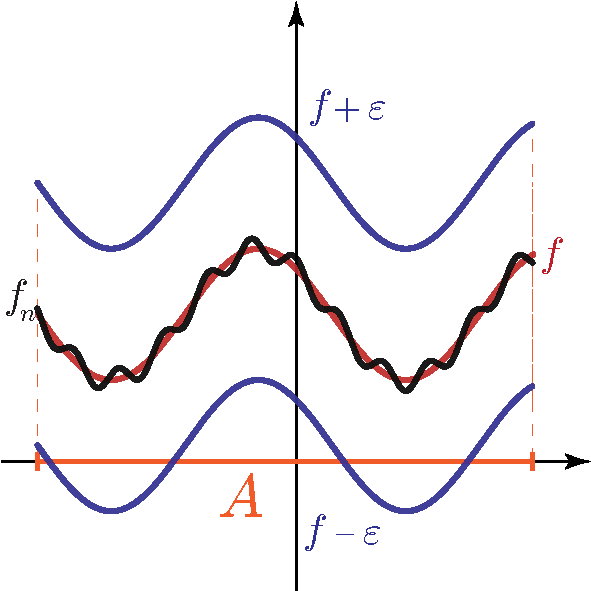
\includegraphics[trim=0cm 0cm 0cm 0cm, clip, scale=0.65]{images/visualizzazioneconvergenzauniforme.pdf}
\end{center}
\paragraph{Convergenza puntuale}
\begin{define}[Convergenza puntuale]
	Consideriamo l'insieme $X$ e le funzioni $\funz{f_n,f}{X}{\complexset}$.
	Si dice che $f_n$ \textbf{converge puntualmente}\index{convergenza!puntuale} a $f$\textbf{in} $X$ ($f_n\overset{\text{punt.}}{\to} f$) se
	\begin{equation}
		\forall x\in X,\lim_{n\to+\infty}f_n(x)=f(x)
	\end{equation}
	o, alternativamente,
	\begin{equation}
		\forall x\in X,\ \forall \epsilon >0,\ \exists N=N\left(x,\epsilon\right)\colon \forall n\geq N,\ \abs{f_n(x)-f(x)}<\epsilon
	\end{equation}
\end{define}
\begin{attention}
	Il limite della convergenza è in campo \textit{complesso}!
\end{attention}
\paragraph{Convergenza uniforme e puntuale}
Come visto in precedenza\footnote{Si veda \refChapterOnly{convergenzafunzioni}, sezione \ref{convuniformeimplicapuntuale}, pag. \pageref{convuniformeimplicapuntuale}.}, nella \textit{convergenza uniforme} il differente ordine dei quantificatori relativi alla $x$ fa sì che la soglia $N$ trovata è indipendente dal punto $x$ e quindi vale per ogni punto dell'insieme di definizione $X$, implicando pertanto la \textit{convergenza puntuale}.
\begin{multline}
	f_n\text{ converge uniformemente a }f\text{ su }X\implies\\
	\implies f_n\text{ converge puntualmente a }f\text{ in ogni punto di }X
\end{multline}
Il viceversa non è vero: abbiamo visto\footnote{Si veda nota precedente.} nella stessa sezione il caso della successione geometrica, la quale converge uniformemente solo a $f\equiv 0$ in ogni intervallo $\left[-a,a\right]\subsetneqq\left(-1,1\right),\ \forall a\in\left(0,1\right)$, mentre puntualmente in tutti i $\left(-1,1\right]$; qui di seguito riportiamo un controesempio alternativo.
\begin{example}
	Consideriamo la successione
	\begin{equation*}
		f_n(x)=\chi_{(n,n+1)}(x)=
		\begin{cases}
			\begin{array}{ll}
				1&n<x<n+1\\
				0&x\leq n\vee x\geq n+1
			\end{array}
		\end{cases}
	\end{equation*}
	Essa converge puntualmente a $f\equiv 0$:
	\begin{itemize}
		\item $\forall x\leq 0$ si ha che $f_n(x)\equiv 0,\ \forall n\in\naturalset$ e dunque banalmente $\displaystyle\lim_{n\to+\infty}f_n(x)=0$.
		\item $\forall x>0$, preso $N_x\coloneqq\floor{x}+1$ si ha che $\forall n>N_x\ f_n(x)=0$ e quindi $\displaystyle\lim_{n\to+\infty}f_n(x)=0$.
	\end{itemize}
	Tuttavia, essa non converge uniformemente a $0$ su $\realset$, dato che
	\begin{equation*}
		\lim_{n\to+\infty}\left(\sup_{x\in\realset}\abs{f_n(x)-f(x)}\right)=\lim_{n\to+\infty}\left(\sup_{x\in\realset}\abs{1-0}\right)=1\neq 0
	\end{equation*}
\end{example}
\paragraph{Convergena quasi ovunque}
\begin{define}[Convergenza quasi ovunque]
	Consideriamo lo spazio di misura $\left(X,\mathcal{M},\mu\right)$ e le funzioni $\funz{f_n,f}{X}{\complexset}$ misurabili per ogni $n$. Si dice che
	$f_n$ \textbf{converge quasi ovunque}\index{convergenza!quasi ovunque} a $f$\textbf{in} $X$ ($f_n\overset{\text{q.o.}}{\to} f$) se
	\begin{equation}
		\mu\left(\left\{x\in X\mid \lim_{n\to+\infty}f_n(x)\neq f(x)\right\}\right)=0
	\end{equation}
\end{define}
\paragraph{Convergenza puntuale e quasi ovunque}
Dalla definizione è evidente che la convergenza \textit{quasi ovunque} nello spazio di misura $X$ è una \textit{convergenza puntuale} in $X$ tolto un insieme di misura nulla. Se in $\left(X,\mathcal{M},\mu\right)$ si ha convergenza puntuale, il sottoinsieme su cui \textit{non} vale è l'insieme vuoto e quindi è banalmente soddisfatta la condizione di convergenza \textbf{q.o.}, ossia
\begin{multline}
	f_n\text{ converge puntualmente a }f\text{ in ogni punto di }X\implies\\
	\implies f_n\text{ converge quasi ovunque a }f\text{ in ogni punto di }X
\end{multline}
Il viceversa non è vero, come possiamo vedere nel seguente esempio.
\begin{example}
	Consideriamo la successione
	\begin{equation*}
		f_n(x)=n\chi_{\left[0,\frac{1}{n}\right]}(x)=
		\begin{cases}
			\begin{array}{ll}
				n&0\leq x\leq\frac{1}{n}\\
				0&x< 0\vee x>\frac{1}{n}
			\end{array}
		\end{cases}
	\end{equation*}
	Osserviamo che la funzione non converge puntualmente a $f(x)=0$ su $\realset$:
	\begin{itemize}
		\item $\forall x< 0$ si ha che $f_n(x)\equiv 0,\ \forall n\in\naturalset$ e dunque banalmente $\displaystyle\lim_{n\to+\infty}f_n(x)=0$.
		\item $\forall x>0$, preso $N_x\coloneqq\frac{1}{x}$ si ha che $\forall n>N_x\ f_n(x)=0$ e quindi $\displaystyle\lim_{n\to+\infty}f_n(x)=0$.
		\item Per $x=0$ si ha $f_n(x)\equiv n,\ \forall n\in\naturalset$ e quindi $\displaystyle\lim_{n\to+\infty}f_n(x)=+\infty\neq0$.
	\end{itemize}
Tuttavia, l'insieme dove $f_n$ \textit{non} converge a $f\equiv0$ è un singolo punto e quindi ha misura nulla, pertanto $f_n$ converge \textbf{q.o.} a $f\equiv 0$.
\end{example}
\paragraph{Convergenza in {$L^1$}}
\begin{define}[Convergenza in {$L^1\left(\mu\right)$}]
	Siano $f_n,f\in L^1\left(\mu\right)$. Si dice che
	$f_n$ \textbf{converge in $L^1\left(\mu\right)$}\index{convergenza!in $L^1\left(\mu\right)$} a $f$ ($f_n\overset{L^1}{\to} f$) se
	\begin{equation}
		\lim_{n\to+\infty}\norm{f_n-f}_1=\lim_{n\to+\infty}\int_{X}\abs{f_n-f}d\mu=0
	\end{equation}
\end{define}
Considerato $X\subseteq \realset$, possiamo visualizzare graficamente la convergenza in $L^1$.
\begin{center}
	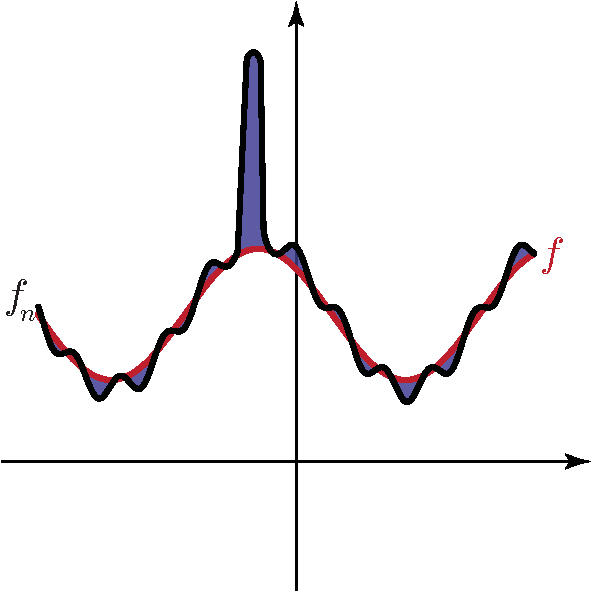
\includegraphics[trim=0cm 0cm 0cm 0cm, clip, scale=0.65]{images/visualizzazioneconvergenzal1.pdf}
\end{center}
Si nota che il grafico di $f_n$ può stare, in qualche zona, molto distante dal grafico di $f$, l'importante è che \textit{complessivamente} l'\textbf{area} tra $f_n$ e $f$ diminuisce, al crescere di $n$, fino ad essere \textit{nulla}.\\
Questa è la differenza principale tra la convergenza uniforme/puntuale/quasi ovunque e quella in $L^1$: se per le prime tre è fondamentale minimizzare la \textit{distanza} tra la funzione $f_n$ e $f$, l'ultima richiede di minimizzare l'\textit{area} tra le due.
\paragraph{Convergenza uniforme e in {$L^1$}}
\begin{theorema}[Legame tra convergenza uniforme e {$L^1$} nel caso di misura finita]
	Consideriamo lo spazio di misura $\left(X,\mathcal{M},\mu\right)$ e le funzione $\funz{f_n,f}{X}{\complexset}$. Se
	\begin{enumerate}[label=(\alph*)]
		\item $f_n\in L^{1}\left(\mu\right)$.
		\item $f_n$ converge uniformemente a $f$ su $X$.
		\item $\mu(X)<+\infty$.
	\end{enumerate}
	allora
	\begin{enumerate}
		\item $f\in L^{1}\left(\mu\right)$.
		\item $\displaystyle\lim_{n\to+\infty}\norm{f_n-f}_1=0$.
		\item Vale il \textbf{passaggio al limite sotto segno di integrale}\index{passaggio al limite sotto segno di integrale}
		\begin{equation}
			\lim_{n\to+\infty}\int_Xf_nd\mu=\int_Xfd\mu
		\end{equation}
	\end{enumerate}
\end{theorema}
\begin{demonstration}~{}
	\begin{enumerate}[label=(\Roman*)]
		\item Dobbiamo dimostrare che $f\in L^!\left(\mu\right)$, ovvero
		\begin{itemize}
			\item $f$ misurabile.
			\item $\displaystyle\int_X\abs{f}d\mu<+\infty$
		\end{itemize}
		Per ipotesi si ha la convergenza uniforme di $f_n$ a $f$ in $X$:
		\begin{equation*}
			\circled[red]{\vardiamond}\quad \forall \epsilon > 0,\ \exists N=N\left(\epsilon\right)\colon \forall n\geq N,\ \abs{f_n(x)-f(x)}<\epsilon,\ \forall x\in X
		\end{equation*}
		Osserviamo che $f$ è dunque misurabile, in quanto la misurabilità passa al limite puntuale (e quindi al limite uniforme). Da $\circled[red]{\vardiamond}$ segue che
		\begin{equation*}
			\abs{f(x)}\underset{=}{\forall n\in\naturalset}\abs{f(x)-f_n(x)+f_n(x)}\leq\abs{f(x)-f_n(x)}+\abs{f_n(x)}\underset{\forall x\in X}{<}\epsilon +\abs{f(x)}
		\end{equation*}
		Posto, ad esempio, $\epsilon = 1$ e $n=N$ si ha
		\begin{equation*}
			\abs{f(x)}=1+\abs{f_N(x)},\ \forall x\in X
		\end{equation*}
		Allora
		\begin{align*}
			\int_X\abs{f}d\mu&\leq \int_X \left(1+\abs{f_N}\right)d\mu&\text{(monotonia integrale per l''integranda)}\\
			&=\int_{X}1d\mu+\int_X\abs{f_N}d\mu&\text{(additività dell'integranda)}\\
			&=\mu(x)+\int_X\abs{f_N}d\mu <+\infty&
		\end{align*}
		perché $\mu(x)<+\infty$ per ipotesi e $f_n\in L^1\left(\mu\right)$.
		\item Dobbiamo dimostrare che $\displaystyle\lim_{n\to+\infty}\norm{f_n-f}_1=0$, ossia
		\begin{equation*}
			\circled[blue]{\spadesuit}\quad \forall \epsilon > 0,\ \exists \widetilde{N}=\widetilde{N}\left(\epsilon\right)\colon \forall n\geq N,\ \norm{f_n(x)-f(x)}_1<\epsilon
		\end{equation*}
		Si ha
		\begin{equation*}
			\norm{f_n-f}_1=\int_X\abs{f_n-f}d\mu\underset{\forall n\geq N\left(\epsilon\right)}{\overset{\circled[red]{\vardiamond}}{\leq}}\int_X\epsilon d\mu=\epsilon \mu(x)<+\infty
		\end{equation*}
		Vale la relazione \circled[blue]{\spadesuit} ponendo $\widetilde{N}=N$.
		\item Segue dal \textit{teorema di convergenza dominata}.
	\end{enumerate}
\end{demonstration}
\begin{attention}
	Se $\mu(x)=+\infty$, in generale \textit{non} vale nessuna delle tesi: come controesempi si possono prendere i tre esposti\footnote{Si veda \refChapterOnly{convergenzafunzioni}, pag. \pageref{controesempipassaggiointegrale}.} nel discorso sui problemi di integrabilità nell'ambito della teoria di Riemann.
\end{attention}
In generale non vale il viceversa: dalla convergenza $L^1$ non segue quella uniforme.
\begin{example}
	Consideriamo la successione
	\begin{equation*}
		f_n(x)=n\chi_{\left[0,\frac{1}{n^2}\right]}(x)=
		\begin{cases}
			\begin{array}{ll}
				n&0\leq x\leq\frac{1}{n^2}\\
				0&x< 0\vee x>\frac{1}{n^2}
			\end{array}
		\end{cases}
	\end{equation*}
	La successione converge in $L^1$ a $f\equiv 0$:
	\begin{equation*}
		\lim_{n\to+\infty}\norm{f_n-f}_1=\lim_{n\to+\infty}\int_{\realset}\abs{f_n-f}d\mu=\lim_{n\to+\infty}\int_{0}^{\frac{1}{n^2}}ndx=\lim_{n\to+\infty}n\cdot\frac{1}{n^2}=\lim_{n\to+\infty}\frac{1}{n}=0
	\end{equation*}
	Tuttavia, essa non converge uniformemente a $0$ su $\realset$, dato che
	\begin{equation*}
		\lim_{n\to+\infty}\left(\sup_{x\in\realset}\abs{f_n(x)-f(x)}\right)=\lim_{n\to+\infty}\left(\sup_{x\in\realset}\abs{n-0}\right)=+\infty\neq 0
	\end{equation*}
\end{example}
\begin{observe}
	Questo teorema ci mostra che il passaggio al limite sotto segno di integrale visto nell'ambito della teoria di Riemann, che contemplava la convergenza uniforme su intervalli limitati, è valido anche nell'ambito della Teoria di Lebesgue.
\end{observe}
Con questo teorema abbiamo finalmente risposto in toto ad uno dei quesiti inizialmente enunciati nel \refChapterOnly{ellipseintroduction}: nell'ambito della teoria di Lebesgue, ci sono tre differenti teoremi per il passaggio al limite sotto il segno di integrale, che sono quelli di
\begin{itemize}
	\item Convergenza uniforme su spazi di misura finita.
	\item Convergenza monotona.
	\item Convergenza dominata.
\end{itemize}
\paragraph{Convergenza in misura}
\begin{define}[Convergenza in misura]
	Consideriamo lo spazio di misura $\left(X,\mathcal{M},\mu\right)$ e le funzione $\funz{f_n,f}{X}{\complexset}$ misurabili per ogni $n$; $\forall n\in\naturalset$ definiamo la funzione $g_n\coloneqq \abs{f_n-f}$. Allora, se prendiamo $\forall n\in\ \naturalset,\forall \epsilon>0$ l'insieme
	\begin{equation*}
		E_{n,\epsilon}\coloneqq g^{-1}_n\left(\left(\epsilon,+\infty\right)\right)=\left\{x\in X\mid \abs{f_n(x)-f(x)}>\epsilon\right\}
	\end{equation*}
	si dice che	$f_n$ \textbf{converge in misura}\index{convergenza!in misura} a $f$ ($f_n\overset{\mu}{\to} f$) se
	\begin{equation}
		\lim_{n\to+\infty}\mu\left(\left\{x\in X\mid \abs{f_n(x)-f(x)}>\epsilon\right\}\right)=0,\ \forall \epsilon >0
	\end{equation}
\end{define}
Considerato $X\subseteq \realset$, possiamo visualizzare graficamente la convergenza in misura.
\begin{center}
	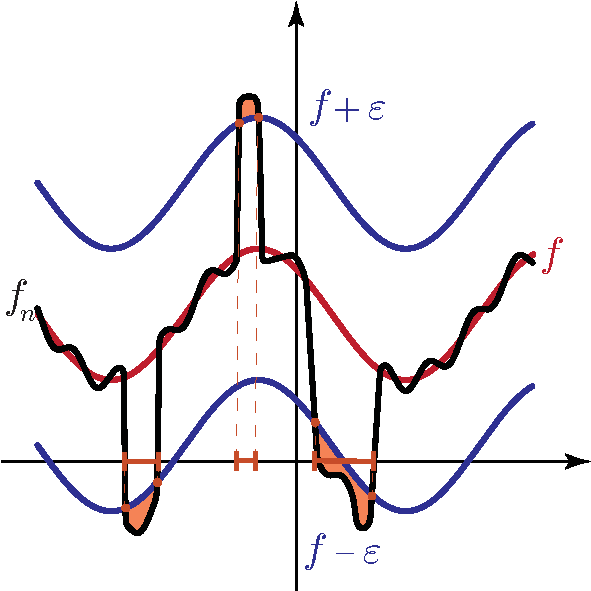
\includegraphics[trim=0cm 0cm 0cm 0cm, clip, scale=0.55]{images/visualizzazioneconvergenzamisura.pdf}
\end{center}
Possiamo interpretare questa convergenza come un particolare tipo di convergenza in $L^1$, condividendo però alcune caratteristiche con la convergenza \textit{uniforme} e alla convergenza \textit{quasi ovunque}. Arbitrariamente scelto un raggio $\epsilon$, il grafico di $f_n$ è nella quasi sua totalità contenuto nell'\textit{intorno tubulare} di raggio $\epsilon$ centrato sul grafico di $f$, ma è concesso che esso possa \textit{uscire} da tale intorno purché la misura dell'insieme di tutti i punti di $\realset$ in cui ciò accade tenda ad essere nulla al crescere di $n$.
\paragraph{Convergenza in {$L^1$} e in misura}
\begin{theorema}[Legame tra convergenza {$L^1$} e convergenza in misura]
	Consideriamo lo spazio di misura $\left(X,\mathcal{M},\mu\right)$ e le funzione $\funz{f_n,f}{X}{\complexset}$ tali che $f_n,f\in L^1\left(\mu\right)$.
	Allora
	\begin{equation}
		f_n\text{ converge in }L^1\text{ a }f\implies f_n\text{ converge in misura a }f
	\end{equation}
\end{theorema}
\begin{demonstration}
	Dobbiamo dimostrare che
	\begin{equation*}
		\mu\bigg(\underbrace{\left\{x\in X\middle|\abs{f_n(x)-f(x)}>\epsilon\right\}}_{\coloneqq E_{n,\epsilon}}\bigg)=0,\ \forall \epsilon>0
	\end{equation*}
	Si ha, per monotonia dell'integrale rispetto al dominio,
	\begin{equation*}
		\int_X\abs{f_n-f}d\mu\geq\int_{E_{n,\epsilon}}\abs{f_n-f}d\mu\geq\epsilon\int_{E_{n,\epsilon}}d\mu=\epsilon\mu\left(E_{n.,\epsilon}\right),\ \forall \epsilon>0,\ \forall n\geq 1
	\end{equation*}
	Dunque si ottiene
	\begin{equation*}
		0\leq \mu\left(E_{n,\epsilon}\right)\leq \frac{1}{\epsilon}\int_X\abs{f_n-f}d\mu=\frac{1}{\epsilon}\underbrace{\norm{f_n-f}_1}_{\substack{\to 0\text{ per }\\n\to+\infty}}
	\end{equation*}
	Passando al limite per $n\to+\infty$, applicando il \textit{teorema del confronto} si ricava:
	\begin{equation*}
		\lim_{n\to+\infty}\mu\left(E_{n,\epsilon}\right)=0,\ \forall \epsilon>0\qedhere
	\end{equation*}
\end{demonstration}
In generale non vale il viceversa: dalla convergenza in misura non segue la convergenza $L^1$.
\begin{example}
	Consideriamo la successione
	\begin{equation*}
		f_n(x)=n\chi_{\left[0,\frac{1}{n}\right]}(x)=
		\begin{cases}
			\begin{array}{ll}
				n&0\leq x\leq\frac{1}{n}\\
				0&x< 0\vee x>\frac{1}{n}
			\end{array}
		\end{cases}
	\end{equation*}
	La successione \textit{non} converge in $L^1$ a $f\equiv 0$:
	\begin{equation*}
		\lim_{n\to+\infty}\norm{f_n-f}_1=\lim_{n\to+\infty}\int_{\realset}\abs{f_n-f}d\mu=\lim_{n\to+\infty}\int_{0}^{\frac{1}{n}}ndx=\lim_{n\to+\infty}n\cdot\frac{1}{n}=\lim_{n\to+\infty}1=1\neq 0
	\end{equation*}
	Tuttavia, essa converge in misura a $0$ su $\realset$, dato che
	\begin{align*}
		&\left\{x\in X\mid \abs{f_n(x)-f(x)}>\epsilon\right\}=\left\{x\in X\mid \abs{f_n(x)}>\epsilon\right\}=\left[0,n\right],\ \forall \epsilon>0\\
		&\implies\lim_{n\to+\infty}\mu\left(\left\{x\in X\mid \abs{f_n(x)-f(x)}>\epsilon\right\}\right)=\lim_{n\to+\infty}\mu\left(\left[0,\frac{1}{n}\right]\right)=\lim_{n\to+\infty}\frac{1}{n}=0,\ \forall \epsilon >0
	\end{align*}
\end{example}
% SVN info for this file
\svnidlong
{$HeadURL$}
{$LastChangedDate$}
{$LastChangedRevision$}
{$LastChangedBy$}

\chapter{Integrali dipendenti da un parametro}
\labelChapter{integralidipendentiparametro}

\begin{introduction}
	‘‘La matematica confronta i più disparati fenomeni e scopre le analogie segrete che li uniscono.''
	\begin{flushright}
		\textsc{Joseph Fourier,} cercando disperatamente di motivare ai suoi genitori la scelta di studiare matematica.
	\end{flushright}
\end{introduction}
\lettrine[findent=1pt, nindent=0pt]{S}{tudieremo} \textbf{[COMPLETARE]}
% TO DO: completare intro
\section{Integrali dipendenti da un parametro}
Nel corso di \textsc{Analisi Matematica 2} abbiamo incontrato gli \textit{integrali dipendenti da un parametro} nella teoria dell'integrazione di Riemann. Espandiamo questo argomento agli integrali di Lebesgue.
\begin{define}[Integrali dipendenti da un parametro]
	Consideriamo lo spazio di misura $\left(\realset,\mathcal{L}\left(\realset\right),m_1\right)$. Un \textbf{integrale dipendente da un parametro}\index{integrale!dipendente da un parametro} è una funzione
	\begin{equation}
		F(t)=\int_I\mvf{f}{t}{x}dm_1(x),\ \forall t\in J
	\end{equation}
	dove $I,J$ sono intervalli in $\realset$ e
	\begin{equation*}
		\funztot{f}{I\times J}{\complexset}{\left(t,x\right)}{\mvf{f}{t}{x}}
	\end{equation*}
	è tale per cui $\forall t\in I\ \funz{f\left(t,\cdot\right)}{J}{\complexset}$ integrabile.
\end{define}
Vogliamo studiare le proprietà di continuità e derivabilità dell'integrale dipendente da una parametro a partire da quelle della funzione $f$ che lo definisce.
\begin{theorema}[Teorema di continuità e derivabilità di integrali dipendenti da un parametro]
	Siano $I,J\subseteq\realset$ intervalli e sia $\funz{f}{I\times J}{\complexset}$ tale che $f\left(t,\cdot\right)$ sia integrabile, $\forall t\in I$. Consideriamo
	\begin{equation*}
		F(t)=\int_I\mvf{f}{t}{x}dm_1(x)
	\end{equation*}
	\begin{enumerate}
		\item Se
		\begin{itemize}
			\item $f\left(\cdot, x\right)$ è continua su $I$, $\forall x\in J$.
			\item $\exists \funz{\phi}{I}{\realset}$ integrabile tale che
			\begin{equation*}
				\abs{\mvf{f}{t}{x}}\leq\phi(x),\ \forall \left(t,x\right)\in I\times J
			\end{equation*}
		\end{itemize}
		allora $F$ è continua su $I$.
		\item Se
		\begin{itemize}
			\item $\exists\frac{\partial f}{\partial t}$ su $I\times J$.
			\item $\exists\funz{\psi}{J}{\realset}$ integrabile tale che
			\begin{equation*}
				\abs{\frac{\partial f}{\partial t}\left(t,x\right)}\leq\psi(x),\ \forall \left(t,x\right)\in I\times J
			\end{equation*}
			allora $F$ è continua su $I$ e si ha la \textbf{derivazione sotto segno di integrale}\index{derivazione sotto segno di integrale}:
			\begin{equation*}
				F'(t)=\int_J\frac{\partial f}{\partial t}\left(t,x\right)dm_1(x), \forall t\in I
			\end{equation*}
		\end{itemize}
	\end{enumerate}
\end{theorema}
Per dimostrare questo teorema ci serviranno i seguenti fatti:
\begin{itemize}
	\item \textbf{Teorema di relazione:} data $\funz{g}{I\subseteq\realset}{\complexset}$ e $\overline{t}\in I$, si ha
	\begin{equation}
		\lim_{t\to\overline{t}}g(t)=L\in\complexset\iff\lim_{n\to+\infty}g\left(t_n\right)=L,\ \forall t_n\to\overline{t}
	\end{equation}
	\item \textbf{Teorema di Lagrange:} data $\funz{g}{I\subseteq\realset}{\complexset}$ derivabile su $I$, si ha
	\begin{equation}
		\forall t_1,t_2\in I, \abs{g\left(t_1\right)-g\left(t_2\right)}\leq\sup_{t\in\left[t_1,t_2\right]}\abs{g'(t)}\abs{t_1-t_2}
	\end{equation}
\end{itemize}
\begin{demonstrationcaputwt}[della continuità e derivabilità di {$F$}]
	\begin{enumerate}[label=\Roman*]
		\item Dobbiamo provare che
		\begin{equation*}
			\forall \overline{t}\in I,\ \lim_{t\to\overline{t}}F(t)=F\left(\overline{t}\right)
		\end{equation*}
		È sufficiente provare che, per il primo fatto enunciato precedentemente,
		\begin{equation*}
			\forall \overline{t}\in I,\ \forall t_n\to\overline{t}, \lim_{n\to+\infty}F\left(t_n\right)=F\left(\overline{t}\right)
		\end{equation*}
		Siano quindi $\overline{t}\in I$ e $t_n\to\overline{t}$ fissati: dobbiamo provare che
		\begin{equation*}
			\lim_{n\to+\infty}\int_Jf\left(t_n,x\right)dm_1(x)=\int_Jf\left(\overline{t},x\right)dm_1(x)
		\end{equation*}
		Ponendo
		\begin{align*}
			g_n(x)\coloneqq f\left(t_n,x\right)\\
			\overline{g}(x)\coloneqq f\left(\overline{t},x\right)
		\end{align*}
		allora la relazione da provare si scrive come
		\begin{equation*}
			\lim_{n\to+\infty}\int_Jg_n(x)dm_1(x)=\int_J\overline{g}(x)dm_1(x)
		\end{equation*}
		ossia ho ottenuto un problema di passaggio al limite sotto segno di integrale. Applichiamo il teorema di convergenza dominata, verificandone le ipotesi:
		\begin{itemize}
			\item \textbf{Convergenza puntuale:}
			\begin{equation*}
				\forall x\in J,\ \lim_{n\to+\infty}g_n(x)=\lim_{n\to+\infty}f\left(t_n,x\right)=f\left(\overline{t},x\right)=\overline{g}(x)
			\end{equation*}
			perché $f\left(\cdot,x\right)$ è continua rispetto alla $t$.
			\item \textbf{Maggiorazione (convergenza dominata):}
			\begin{equation*}
				\abs{g_n(x)}\underset{\substack{\forall n\geq 1\\\forall x\in J}}{=}\abs{f\left(t_n,x\right)}\leq \phi(x)\quad\text{(indipendentemente da $n$)}
			\end{equation*}
		\end{itemize}
		Si può allora passare al limite sotto segno di integrale e concludere.
		\item Dobbiamo provare che
		\begin{equation*}
			F'(t)=\int_J\frac{\partial f}{\partial t}\left(\overline{t},x\right)dm_1(x),\ \forall \overline{t}\in I
		\end{equation*}
		ossia
		\begin{equation*}
			\lim_{t\to\overline{t}}\frac{F(t)-F\left(\overline{t}\right)}{t-\overline{t}}=\int_J\frac{\partial f}{\partial t}\left(\overline{t},x\right)dm_1(x),\ \forall \overline{t}\in I
		\end{equation*}
		Per il primo dei fatti è sufficiente provare che
		\begin{equation*}
			\lim_{n\to+\infty}\frac{F\left(t_n\right)-F\left(\overline{t}\right)}{t_n-\overline{t}}=\int_J\frac{\partial f}{\partial t}\left(\overline{t},x\right)dm_1(x),\ \forall \overline{t}\in I,\ \forall t_n\to \overline{t}
		\end{equation*}
		Siano allora $\overline{t}\in I$ e $t_n\to\overline{t}$ fissati: dobbiamo provare che
		\begin{align*}
			\lim_{n\to+\infty}\frac{F\left(t_n\right)-F\left(\overline{t}\right)}{t_n-\overline{t}}&=\lim_{n\to+\infty}\frac{1}{t_n-\overline{t}}\left(\int_Jf\left(+t_n,x\right)dm_1(x)-\int_Jf\left(\overline{t},x_n\right)dm_1(x)\right)=\\
			&=\lim_{n\to+\infty}\int_J\underbrace{\frac{f\left(t_n,x\right)-f\left(\overline{t},x\right)}{t_n-\overline{t}}}_{\coloneqq h_n(x)}dm_1(x)=\int_J\underbrace{\frac{\partial f}{\partial t}\left(\overline{t},x\right)}_{\coloneqq \overline{h}(x)}dm_1(x)
		\end{align*}
		ottenendo
		\begin{equation*}
			\lim_{n\to+\infty}\int_Jh_n(x)dm_1(x)=\int_J\overline{h}(x)dm_1(x)
		\end{equation*}
		ossia ho di nuovo un problema di passaggio al limite sotto segno di integrale. Come prima, applichiamo il teorema di convergenza dominata, verificandone le ipotesi:
		\begin{itemize}
			\item \textbf{Convergenza puntuale:}
			\begin{equation*}
				\forall x\in J,\ \lim_{n\to+\infty}h_n(x)=\overline{h}(x)
			\end{equation*}
			per definizione di derivata parziale.
			\item \textbf{Maggiorazione (convergenza dominata):}
			\begin{equation*}
				\abs{h_n(x)}\underset{\substack{\forall n\geq 1\\\forall x\in J}}{=}\abs{\frac{f\left(t_n,x\right)-f\left(\overline{t},x\right)}{t_n-t}}\underset{\text{fatto }2}{\leq} \frac{\displaystyle\sup_{t\in\left[t_n,\overline{t}\right]}\abs{\frac{\partial f}{\partial t}}\Ccancel[red]{\abs{t_n-\overline{t}}}}{\Ccancel[red]{\abs{t_n-\overline{t}}}}\leq \psi(x)
			\end{equation*}
		\end{itemize}
		Si può allora passare al limite sotto segno di integrale e concludere.\qedhere
	\end{enumerate}
\end{demonstrationcaputwt}
\section{La trasformata di Fourier}
\begin{define}[Trasformata di Fourier]
	Sia $\funz{g}{\realset}{\realset}$. Data la funzione
	\begin{equation*}
		\mvf{f}{t}{x}=g(x)e^{-itx},\ \forall \left(t,x\right)\in\realset^2,
	\end{equation*}
	dove
	\begin{equation*}
		e^{-itx}=\cos tx-i\sin tx,\ \forall\left(t,x\right)\in\realset^2,
	\end{equation*}
	definiamo la \textbf{trasformata di Fourier}\index{trasformata di Fourier} di $g$ l'integrale dipendente dal parametro di $t$ dato da $f$:
	\begin{equation}
		\begin{array}{ll}
			\displaystyle\hat{g}(t)&=\displaystyle\int_{\realset}g(x)e^{-itx}dm_1(x)=\\
			&=\displaystyle\int_{\realset}g(x)\cos txdm_1(x)-i\int_\realset g(x)\sin txdm_1(x),\ \forall t\in\realset
		\end{array}
	\end{equation}
\end{define}
Ci chiediamo sotto quali ipotesi su $g$ la funzione $F$ è continua e sotto quali invece è derivabile.
\begin{theorema}[Continuità e derivabilità della trasformata di Fourier]
	Sia data $\funz{g}{\realset}{\realset}$.
	\begin{enumerate}
		\item Se $g\in L^1\left(\realset\right)$, allora $\hat{g}$ è continua su $\realset$.
		\item Se
		\begin{itemize}
			\item $g\in L^1\left(\realset\right)$.
			\item $xg(x)\in L^1\left(\realset\right)$.
		\end{itemize}
		allora $\hat{g}$ è derivabile su $\realset$ e
		\begin{equation}
			\hat{g}'(t)=\widehat{\left(-ixg(x)\right)}=-i\int_{\realset}xg(x)e^{-itx}dm_1(x),\ \forall t\in\realset
		\end{equation}
	\end{enumerate}
\end{theorema}
\begin{demonstration}~
	\begin{enumerate}[label=\Roman*]
		\item % TO DO: completare
		\item Applichiamo il teorema di derivabilità degli integrali dipendenti da un parametro. In questo caso si ha
		\begin{equation*}
			\mvf{f}{t}{x}=g(x)e^{-itx},\ \forall \left(t,x\right)\in\realset^2
		\end{equation*}
		Verifichiamo le ipotesi.
		\begin{itemize}
			\item $\mvf{f}{t}{\cdot}$ è integrabile su $\realset$:
			\begin{itemize}
				\item $\mvf{f}{t}{\cdot}$ misurabile perché $f$ è il prodotto di $g$ e $e^{-itx}$, due funzioni misurabili - la prima per ipotesi, la seconda in quanto è continua.
				\item $\displaystyle\int_{\realset}\abs{\mvf{f}{t}{x}}<+\infty$ in quanto
				\begin{equation*}
					\abs{\mvf{f}{t}{x}}=-ixg(x)e^{-itx},\ \forall \left(t,x\right)\in\realset^2
				\end{equation*}
			\end{itemize}
			\item Esiste
			\begin{equation*}
				\frac{\partial f}{\partial t}=-ixg(x)e^{itx},\ \forall \left(t,x\right)\in\realset^2
			\end{equation*}
			\item Si può maggiorare uniformemente $\dfrac{\partial f}{\partial t}$ in $t$ con una funzione integrabile:
			\begin{equation*}
				\abs{\frac{\partial f}{\partial t}\left(t,x\right)}=\abs{-ixg(x)e^{-itx}}=\abs{xg(x)}\underbrace{\abs{e^{-itx}}}_{=1}=\abs{xg(x)}\coloneqq \psi(x),\ \forall \left(t,x\right)\in\realset^2
			\end{equation*}
			con $\psi(x)$ integrabile per ipotesi sull'integrabilità di $xg(x)$.
		\end{itemize}
		Ne segue che $\hat{g}$ è derivabile e
		\begin{equation*}
			\hat{g}'(t)=\int_{\realset}\frac{\partial f}{\partial t}\left(t,x\right)dm_1(x)=-i\int_{\realset}xg(x)e^{-itx}dm_1(x)\qedhere
		\end{equation*}
	\end{enumerate}
\end{demonstration}
% SVN info for this file
\svnidlong
{$HeadURL$}
{$LastChangedDate$}
{$LastChangedRevision$}
{$LastChangedBy$}

\chapter{Analisi e probabilità}
\labelChapter{analisiprobabilità}

\begin{introduction}
	‘‘Se il tuo esperimento richiede di usare la statistica, dovevi fare un esperimento migliore.''
	\begin{flushright}
		\textsc{Ernest Rutherford,} stanco di studiare Calcolo delle Probabilità e Statistica.
	\end{flushright}
\end{introduction}
\lettrine[findent=1pt, nindent=0pt]{C}{ome} abbiamo potuto notare nel corso di \textsc{Calcolo di Probabilità}, la teoria della \textbf{probabilità} si è notevolmente espansa dal mero studio di eventi discreti con metodi combinatoriali. Infatti, Andrey Nikolaevich \textbf{Kolmogorov} (1903 – 1987) nel 1933 combinò la nozione di spazio campione, già introdotta da Richard \textbf{von Mises} (1883 – 1953), e la teoria della misura di Lebesgue per definire un sistema assiomatico compatibile sia con la teoria \textit{classica} della probabilità, sia con l'\textit{Analisi moderna}: in questo modo, gli eventi potevano essere anche un qualcosa di \textit{continuo}, con tutto ciò che ne consegue.\\
In questo ultimo capitolo di teoria approfondiremo alcuni concetti visti a \textsc{Calcolo di Probabilità} con il formalismo e il rigore dato dalla teoria della Misura e dell'integrazione. Partiremo con l'enunciare gli \textit{assiomi di probabilità} di Kolmogorov per poi dedicarci a come studiare le \textit{variabili aleatorie} tramite la sola \textit{probabilità immagine}, e in base ad essa dare una classificazione \textit{esaustiva} delle variabili aleatorie. Concludiamo la trattazione rivedendo i \textit{modi di convergenza} delle funzioni misurabili in ambito probabilistico.
\section{Spazio di probabilità e variabili aleatorie}
\begin{define}[Spazio di probabilità]
	Uno \textbf{spazio di probabilità}\index{spazio!di probabilità} $\left(\Omega,\mathcal{F},\mathbb{P}\right)$ è una struttura matematica che fornisce un modello formale per un esperimento non deterministico. Essa costituita dai seguenti elementi:
	\begin{enumerate}
		\item Uno \textbf{spazio campionario}\index{spazio!campionario} $\Omega$, l'insieme di tutti i possibili \textbf{risultati} $\omega$ dell'esperimento.
		\item Uno \textbf{spazio degli eventi}\index{spazio!degli eventi} $\mathcal{F}$, la famiglia di tutti gli eventi dell'esperimento, dove un \textbf{evento}\index{evento} $E$ è un insieme di risultati dello spazio campionario - ossia un sottoinsieme di $\Omega$.
		\item Una \textbf{funzione di probabilità} $\mathbb{P}$, che assegna ad ogni evento una probabilità, la quale è un numero tra 0 e 1.
		\begin{equation}
			\funz{\mathbb{P}}{\mathcal{F}}{\left[0,1\right]}
		\end{equation}
	\end{enumerate}
\end{define}
Questo spazio di probabilità deve soddisfare gli assiomi di probabilità introdotti da Andrey Kolmogorov nel 1933.
\begin{axiom}[Primo assioma di probabilità]
	La probabilità di un evento è un numero reale non negativo.
	\begin{equation}
		\mathbb{P}\left(E\right)\in\realset,\ \mathbb{P}\left(E\right)\geq 0\quad \forall E\in\mathcal{F} 
	\end{equation}
\end{axiom}
\begin{axiom}[Secondo assioma di probabilità]
	La probabilità dello spazio campionario è $1$.
	\begin{equation}
		\mathbb{P}\left(\Omega\right)=1
	\end{equation}
\end{axiom}
\begin{axiom}[Terzo assioma della probabilità]
	La probabilità è $\sigma$-additiva:	$\forall A_n\in\mathcal{F}$ tali che $A_i\cap A_j=\emptyset\ \forall i\neq j$, allora
	\begin{equation}
		\mathbb{P}\left(\coprod_{n\geq 1}A_n\right)=\sum_{n\geq 1}\mathbb{P}\left(A_n\right)
	\end{equation}
\end{axiom}
\begin{proposition}[L'insieme vuoto ha probabilità nulla]
	Sia $\left(\Omega,\mathcal{F},\mathbb{P}\right)$ uno spazio di probabilità. Allora l'insieme vuoto ha probabilità nulla.
\end{proposition}
\begin{demonstration}
	Consideriamo la successione di eventi seguente:
	\begin{equation*}
		A_n=\begin{cases}
			\begin{array}{ll}
				\Omega&n=1\\
				\emptyset&n\geq2
			\end{array}
		\end{cases}
	\end{equation*}
	Osserviamo che $\Omega\cap \emptyset=\emptyset$ e $\emptyset\cap\emptyset=0$; poiché
	\begin{equation*}
		\Omega=\bigcup_{n\geq 1}A_n,
	\end{equation*}
	applichiamo l'assioma 3, la $\sigma$-additività all'unione degli $A_n$:
	\begin{align*}
		1&=\mathcal{P}\left(\Omega\right)=\mathcal{P}\left(\bigcup_{n\geq 0}A_n\right)=\sum_{n\geq 1}\mathbb{P}\left(A_n\right)=\mathbb{P}\left(A_1\right)+\sum_{n\geq2}\mathbb{P}\left(A_n\right)&\\
		&=\mathbb{P}\left(\Omega\right)+\sum_{n\geq 2}\mathbb{P}\left(\emptyset\right)&\text{(Assioma 1)}\\
		&=1-\sum_{n\geq 2}\mathbb{P}\left(\emptyset\right)&
	\end{align*}
	da cui
	\begin{equation*}
		\sum_{n\geq 2}\mathbb{P}\left(\emptyset\right)=0
	\end{equation*}
	Poiché per il primo assioma la probabilità di un evento è sempre non-negativa, ne consegue che ogni elemento di questa sommatoria debba essere uguale a zero, ossia $\mathcal{P}\left(\emptyset\right)=0$.
\end{demonstration}
Si può subito osservare che lo spazio di probabilità $\left(\Omega,\mathcal{F},\mathbb{P}\right)$ altro non è che uno \textbf{spazio di misura} $\left(X,\mathcal{M},\mu\right)$, con l'ipotesi aggiunta che la misura $\mu$ sia di \textbf{probabilità}, cioè $\mu(X)=1$.
\begin{define}[Funzione misurabile]
	Sia $\left(\Omega,\mathcal{F},\mathbb{P}\right)$ uno spazio di probabilità. Una funzione $\funz{X}{\Omega}{\complexset}$ si dice \textbf{variabile aleatoria}\index{variabile aleatoria} se \begin{equation}
		X^{-1}\left(A\right)\in\mathcal{F},\ \forall A\subseteq \complexset\text{ aperto.}
	\end{equation}
\end{define}
In altre parole, una variabile aleatoria è una funzione misurabile da uno spazio di probabilità a $\complexset$.
\section{Probabilità immagine}\label{probimm}
Nel corso di \textsc{Calcolo di Probabilità} abbiamo incontrato la variabile aleatoria \textbf{normale standard} $Z$, definita come tale se la probabilità che $Z$ stia nell'evento $B$ è
\begin{equation}
	\mathbb{P}\left(Z\in B\right)=\int_{B}\frac{1}{\sqrt{2\pi}}e^{-x^2/2}dm_1,\ \forall B\in\mathcal{B}\left(\realset\right)
\end{equation}
Le variabili aleatorie, per definizione, sono funzioni da uno spazio di probabilità $\Omega$ a valori - in questo caso - reali. La definizione della normale standard, tuttavia, non fa alcun riferimento allo spazio di probabilità. Cos'è dunque  $\left(\Omega,\mathcal{F},\mathbb{P}\right)$?\\
In realtà \textit{non si sa}, ma non ci interessa individuarlo. Motiviamo questa affermazione audace introducendo il concetto di \textit{misura immagine}, visto nell'ambito di Teoria della probabilità come \textit{probabilità immagine}.
\begin{define}[Misura immagine]
	Siano $\left(X,\mathcal{F}\right)$ e $\left(Y,\mathcal{M}\right)$ due spazi misurabili e una funzione $\funz{f}{X}{Y}$ misurabile. Se su $\left(X,\mathcal{F}\right)$ consideriamo una misura $\funz{\mu}{\mathcal{F}}{\left[0,+\infty\right]}$, la \textbf{misura immagine}\index{misura!immagine} o \textbf{pushforward}\index{misura!pushforward} è la misura $\funz{f_{\ast}\left(\mu\right)}{\mathcal{M}}{\left[0,+\infty\right]}$ definita da
	\begin{equation}
		\left[f_{\ast}\left(\mu\right)\right]\left(B\right)=\mu\left(f^{-1}\left(B\right)\right),\ \forall B\in \mathcal{M}
	\end{equation}
\end{define}
\begin{theoremaqed}[Integrazione con cambio di variabili tramite pushforward]
	Data una funzione $g$ su $Y$ misurabile, allora
	\begin{equation}
		g\in L^{1}\left(f_{\ast}\left(\mu\right)\right)\iff g\circ f\in L^{1}\left(\mu\right),
	\end{equation}
	ossia
	\begin{equation}
		\int_{X}g\circ fd\mu=\int_{Y}gd\left(f_{\ast}\left(\mu\right)\right)\qedhere
	\end{equation}
\end{theoremaqed}
Interpretiamo questo nuovo concetto nell'ambito degli spazi di probabilità.
\begin{define}[Probabilità immagine]
	Sia $\left(X,\mathcal{M},\mathbb{P}\right)$ e spazio di probabilità e $\funz{X}{\Omega}{\realset}$ variabile aleatoria.
	La \textbf{probabilità immagine}\index{probabilità!immagine} è la misura di probabilità $\funz{\mathbb{P}_X}{\mathcal{B}\left(\realset\right)}{\left[0,1\right]}$ definita da
	\begin{equation}
		\mathbb{P}_X\left(B\right)=\mathbb{P}\left(X^{-1}\left(B\right)\right),\ \forall B\in \mathcal{B\left(\realset\right)}
	\end{equation}
	e definisce un nuovo spazio di probabilità $\left(\realset,\mathcal{B}\left(\realset\right),\mathbb{P}_X\right)$.
\end{define}
\begin{theoremaqed}[Integrazione con cambio di variabili tramite probabilità immagine]
	Data una funzione $g$ su $\realset$ misurabile, allora
	\begin{equation}
		\circled[blue]{\spadesuit}\quad g\in L^{1}\left(\mathbb{P}_X\right)\iff g\circ X\in L^{1}\left(\mathbb{P}\right),
	\end{equation}
	ossia
	\begin{equation}
		\int_{\Omega}g(x)d\mathbb{P}=\int_{\realset}gd\mathbb{P}_X\qedhere
	\end{equation}
\end{theoremaqed}
\begin{center}
	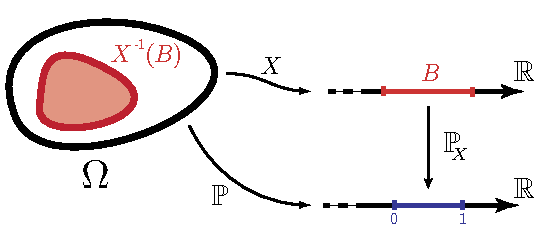
\includegraphics[width=0.4\paperwidth]{images/probimmagine}
\end{center}
Pertanto, non mi interessa nello specifico sapere cos'è $\Omega$ o com'è definita $\mathbb{P}$: se definisco la variabile aleatoria direttamente con la probabilità immagine ‘‘dimentico'' quale fosse lo spazio originale e lavoro direttamente su $\realset$.
\begin{define}[Momento di ordine {$k$-esimo}]
	Se consideriamo la funzione $g(x)=x^k,\ \forall x\in\realset$ e $\forall k\in\naturalset$, si definisce il \textbf{momento}\index{momento di ordine {$k$}-esimo} il valore
	\begin{equation*}
		\mathbb{E}\left(X^k\right)=\int_{\Omega}X^kd\mathbb{P}=\int_{\realset}x^kd\mathbb{P}_X
	\end{equation*}
\end{define}
\section{Funzione di ripartizione e classificazione delle variabili aleatorie}
\begin{define}[Funzione di ripartizione]
	Siano $\left(\Omega,\mathcal{M},\mathbb{P}\right)$ uno spazio di probabilità, $\funz{X}{\Omega}{\realset}$ una variabile aleatoria e $\mathbb{P}_X$ la corrispondente probabilità immagine. Si chiama \textbf{funzione di ripartizione}\index{funzione!di ripartizione} (abbreviata in \textbf{cdf}, dall'inglese \textit{cumulative distributive function}) la funzione $\funz{F_X}{\realset}{\left[0,1\right]}$ definita da
	\begin{equation}
		F_X(x)=\mathbb{P}_X\left(\left(-\infty,x\right]\right)=\mathbb{P}\left(X\leq x\right),\ \forall x\in\realset
	\end{equation}
\end{define}
Una funzione di ripartizione $F_X$ soddisfa le seguenti proprietà:
\begin{enumerate}
	\item È monotona non decrescente.
	\item È continua a destra.
	\item È tale per cui
	\begin{equation}
		\lim_{x\to+\infty}F_X(x)=0\quad\lim_{x\to+\infty}F_X(x)=1
	\end{equation}
	ossia ha immagine $\left[0,1\right]$.
\end{enumerate}
Vale anche il viceversa: una funzione che soddisfa queste caratteristiche è una funzione di ripartizione per qualche variabile aleatoria.\\
La variabili aleatorie si classificano in base alla probabilità immagine $\mathbb{P}_X$ e, di conseguenza, alla funzione di ripartizione $F_X$, in una delle quattro classi seguenti:
\begin{itemize}
	\item V.a. \textit{assolutamente continue}.
	\item V.a. \textit{singolari discrete}.
	\item V.a. \textit{singolari continue}.
	\item V.a. \textit{miste}.
\end{itemize}
\subsection{Variabili aleatorie assolutamente continue}
\begin{define}[V.a. assolutamente continua e densità]
	$X$ si dice variabile aleatoria \textbf{assolutamente continua}\index{variabile aleatoria!assolutamente continua} se $\mathbb{P}_X$ è assolutamente continua rispetto alla misura di Lebesgue $m_1$:
	\begin{equation}
		\forall E\in\mathcal{B}\left(\realset\right),\ m_1\left(E\right)=0\implies \mathbb{P}_X\left(E\right)=0
	\end{equation}
	Per il \textit{teorema di Radon-Nikodym} esiste quindi una funzione detta \textbf{densità} $f\in\mathcal{L}^1\left(\realset\right)$, $f\geq 0$ tale che
	\begin{equation}
		\mathbb{P}_X\left(B\right)=\int_B fdm_1,\ \forall B\in\mathcal{B}\left(\realset\right)
	\end{equation}
\end{define}
Abbiamo già visto\footnote{Si veda \refChapterOnly{integraledilebesgue}, pag. \pageref{misuraindotta}.} come integrare delle funzioni rispetto ad una misura indotta da un'altra misura, come qui è il caso.
\begin{theoremaqed}[Integrazione di funzioni rispetto a v.a. assolutamente continue]
	Data una funzione $g$ su $\realset$, allora
	\begin{equation}
		g\in L^{1}\left(\mathbb{P}_X\right)\iff fg\in L^{1}\left(m_1\right),
	\end{equation}
	ossia
	\begin{equation}
		\int_{\realset}gd\mathbb{P}_X=\int_{\realset}fgdm_1\qedhere
	\end{equation}
\end{theoremaqed}
\begin{define}[Momento di una ordine {$k$-esimo} di v.a. assolutamente continue]
	Sia $X$ una v.a. assolutamente continua di densità $f$. Se consideriamo la funzione $g(x)=x^k,\ \forall x\in\realset$ e $\forall k\in\naturalset$, si definisce il \textbf{momento}\index{momento di ordine {$k$}-esimo} il valore
	\begin{equation*}
		\mathbb{E}\left(X^k\right)=\int_{\Omega}X^kd\mathbb{P}=\int_{\realset}x^kd\mathbb{P}_X=\int_{\realset}x^kd\mathbb{P}_X=\int_{\realset}x^kfdm_1
	\end{equation*}
\end{define}
\begin{examplewt}[Variabile aleatoria normale]
	Approfondendo ciò ad inizio della sezione \ref{probimm}. La variabile aleatoria \textbf{normale standard}\index{variabile aleatoria!normale standard} è una variabile aleatoria $\funz{Z}{\Omega}{\realset}$ di cui è ignoto lo spazio di probabilità $\left(\Omega,\mathcal{M},\mathbb{P}\right)$; tuttavia, essa è definita attraverso la probabilità immagine $\mathbb{P}_X$ assolutamente continua rispetto alla misura $m_1$ associata alla densità Gaussiana:
	\begin{equation}
		\mathbb{P}\left(X\in\mathbb{B}\right)=\mathbb{P}_X\left(B\right)=\int_B\frac{1}{\sqrt{2\pi}}e^{-x^2/2}dm_1,\ \forall B\in\mathcal{B}\left(\realset\right)
	\end{equation}
	I momenti della v.a. normale standard sono
	\begin{equation*}
		\mathbb{E}X^k=\int_{\Omega}X^kd\mathbb{P}=\int_{\realset}x^kd\mathbb{P}_X=\int_{\realset}x^k\frac{1}{\sqrt{2\pi}}e^{-x^2/2}dm_1
	\end{equation*}
\end{examplewt}
\paragraph{Cdf di v.a. assolutamente continue}
La funzione di ripartizione $\funz{F_X}{\realset}{\left[0,1\right]}$ di una variabile aleatoria assolutamente continua è una funzione \textbf{assolutamente continua}.
\begin{center}
	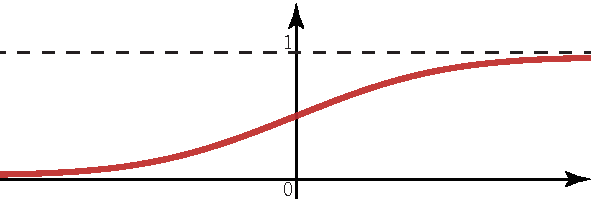
\includegraphics[width=0.4\paperwidth]{images/vacontinua}
\end{center}
\begin{define}[Assoluta continuità.]
	Una funzione $\funz{f}{\realset}{\realset}$ è assolutamente continua se
	\begin{gather*}
		\forall \epsilon>0,\ \exists \delta >0\colon \forall \left(a_1,b_1\right),\ \dots,\ \left(a_n,b_n\right),\ \left(a_i,b_i\right)\cap\left(a_j,b_j\right)=\emptyset,\ \forall i\neq j,\\
		\sum_{i=1}^{n}\abs{b_i-a_i}<\delta\implies\sum_{i=1}^{n}\abs{f\left(b_i\right)-f\left(a_i\right)}<\epsilon
	\end{gather*}
\end{define}
\begin{observe}
	Scegliendo un unico intervallo $\left(a_1,b_1\right)$ si ritrova la definizione di \textit{uniforme continuità}. Pertanto, l'assoluta continuità è una condizione più forte dell'uniforme continuità e in quanto tale implica anche la continuità della funzione originale.
\end{observe}
Ricordiamo che
\begin{equation*}
	F_X(x)=\mathbb{P}_X\left(\left(-\infty,x\right]\right)=\int_{\left(-\infty,x\right]}fdm_1
\end{equation*}
Si dimostra che $F_X$ è derivabile \textbf{q.o.} e che vale
\begin{equation}
	F'_X(x)=f(x),\ \textrm{per quasi ogni }x\in\realset
\end{equation}
Questa relazione non è altro che l'\textbf{estensione del teorema fondamentale del calcolo integrale alla teoria di Lebesgue}\index{teorema!fondamentale del calcolo integrale nella teoria di Lebesgue}.
\subsection{Misure singolari}
Consideriamo una misura $\funz{\lambda}{\mathcal{B}\left(\realset\right)}{\left[0,+\infty\right]}$ non assolutamente continua rispetto alla misura di Lebesgue $m_1$.
Negare
\begin{equation*}
	\forall E\in\mathcal{B}\left(\realset\right)\colon m_1\left(E\right)=0\implies \lambda\left(E\right)=0
\end{equation*}
significa che esiste un insieme $S\in\mathcal{B}\left(\realset\right)$ tale che
\begin{equation*}
	m_1\left(S\right)=0\text{ ma }\lambda\left(S\right)\neq 0
\end{equation*}
In particolare, se vale
\begin{equation*}
	\lambda\left(S\right)=\lambda\left(\realset\right)
\end{equation*}
la misura viene chiamata \textit{singolare} e si definisce \textit{concentrata} in $S$
\begin{define}[Misura singolare]
	Dato un spazio di misura $\left(X,\mathcal{M},\mu\right)$, una misura $\funz{\lambda}{\mathcal{M}}{\left[0,+\infty\right]}$ non assolutamente continua rispetto a $\mu$ si dice \textbf{singolare}\index{misura!singolare} rispetto a $\mu$ se
	\begin{equation}
		\exists S\in\mathcal{M}\colon \mu\left(S\right)=0, \lambda\left(S\right)\neq0 \text{ ma }\lambda(X)=\lambda\left(S\right)
	\end{equation}
	La misura $\lambda$ è detta \textbf{concentrata} in $S$ e si indica con $\mu\perp\lambda$.
	\begin{itemize}
		\item Se $\lambda$ è concentrata in $S$ insieme numerabile, allora $\lambda$ è detta \textbf{singolare discreta}\index{misura!singolare!discreta} o \textbf{atomica}\seeonlyindex{misura!singolare!atomica}{misura!singolare!discreta}.
		\item Se $\lambda$ è concentrata in $S$ insieme \textit{non} numerabile, $\lambda$ è detta \textbf{singolare continua}\index{misura!singolare!continua}.
	\end{itemize}
\end{define}
\begin{observe}
	Si può vedere che se prendo $A\subseteq S^{C}=X\setminus S$, allora $\lambda\left(A\right)=0$, in quanto se così non fosse si avrebbe $\lambda\left(S\right)\neq\lambda(X)$. Si osserva chiaramente che vale anche il viceversa per $\mu$: se prendo $B\subseteq S$, allora $\mu\left(B\right)=0$.\\
	Da ciò, si vede una definizione alternativa per le misura singolari: una misura $\lambda$ singolare rispetto a $\mu$ se esiste un insieme $S\in\mathcal{M}$ tale che $\mu\left(A\right)=0,\ \forall A\subseteq S$ misurabili e $\lambda\left(B\right)=0,\ \forall A\subseteq S^{C}$ misurabili.
\end{observe}
\subsection{Variabili aleatorie singolari discrete}
\begin{define}[Variabili aleatorie singolari discrete]
	$X$ si dice variabile aleatoria \textbf{singolare discreta}\index{variabile aleatoria!singolare!discreta} o \textbf{atomica}\seeonlyindex{variabile aleatoria!singolare!atomica}{variabile aleatoria!singolare!discreta} se $\mathbb{P}_X$ è \textbf{singolare discreta} rispetto alla misura di Lebesgue $m_1$.\\
	Per definizione di misura singolare discreta, esiste $S=\left\{\omega_n\right\}_{n\geq 1}$ tale che, posto
	\begin{equation}
		p_n=\mathbb{P}_X\left(\left\{\omega_n\right\}\right),\ \forall n\geq 1,
	\end{equation}
	si ha
	\begin{equation}
		\mathbb{P}\left(B\right)=\sum_{n\colon\omega_n\in B}p_n,\ \forall B\in\mathcal{B}\left(\realset\right)
	\end{equation}
\end{define}

\begin{theoremaqed}[Integrazione di funzioni rispetto a v.a. singolari discrete]
	Data una funzione $g$ su $\realset$, allora
	\begin{equation}
		g\in L^{1}\left(\mathbb{P}_X\right)\iff \sum_{n=1}^{+\infty}\abs{g\left(\omega_n\right)}p_n<+\infty
	\end{equation}
	e
	\begin{equation}
		\int_{\realset}gd\mathbb{P}_X=\sum_{n=1}^{+\infty}g\left(\omega_n\right)p_n\qedhere
	\end{equation}
\end{theoremaqed}
Abbiamo già dimostrato questo teorema parlando dell'integrazione rispetto ad una misura conteggio pesata\footnote{Si veda \refChapterOnly{integraledilebesgue}, teorema \ref{integrazionemisuraconteggiopesata}, pag. \pageref{integrazionemisuraconteggiopesata}.}.
\paragraph{Cdf di v.a. singolari discrete}
La funzione di ripartizione $\funz{F_X}{\realset}{\left[0,1\right]}$ di una variabile aleatoria singolare discreta è una funzione \textbf{costante a tratti}.
\begin{center}
	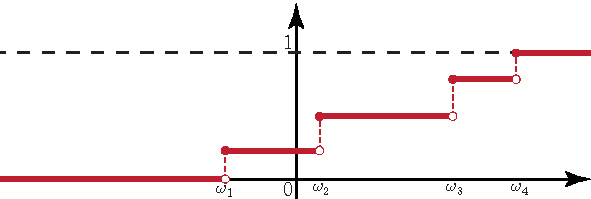
\includegraphics[width=0.4\paperwidth]{images/vadiscreta}
\end{center}
In particolare, $S$ è l'insieme delle discontinuità di $F_X$ e vale
\begin{equation}
	p_n=\lim_{x\to\omega_n^{+}}F_X(x)-\lim_{n\to\omega_n^{-}}F_X(x),\ \forall n\geq 1
\end{equation}
\subsection{Variabili aleatorie singolari continue}
\begin{define}[Variabili aleatorie singolari continue]
	$X$ si dice variabile aleatoria \textbf{singolare continua}\index{variabile aleatoria!singolare!continua} se $\mathbb{P}_X$ è \textbf{singolare continua} rispetto alla misura di Lebesgue $m_1$.\\
	Per definizione di misura singolare continua, esiste $S$ non numerabile con misura di Lebesgue nulla tale che,
	\begin{equation}
		\mathbb{P}_X\left(S\right)=1
	\end{equation}
\end{define}
\paragraph{Cdf di v.a. singolari continua}
La funzione di ripartizione $\funz{F_X}{\realset}{\left[0,1\right]}$ di una variabile aleatoria singolare continua è una funzione \textbf{continua} ma non \textit{assolutamente continua}.\\
In particolare, si dimostra che $F_X$ è derivabile su $\realset\setminus S$ (ossia \textbf{q.o.}) e
\begin{equation}
	F'_X(x)=0,\ \forall x\in\realset\setminus S
\end{equation}
\begin{observe}
	Questa condizione è compatibile con il fatto che $F_X$ sia crescente ed abbia come immagine $\left[0,1\right]$.
\end{observe}
\begin{examplewt}[Distribuzione di Cantor]
Una funzione ha la \textbf{distribuzione di Cantor}\index{distribuzione!di Cantor} se la sua funzione di ripartizione è la \textit{funzione di Cantor}\footnote{Si veda \refChapterOnly{teoriamisura}, teorema \ref{funzionecantor}, pag. \pageref{funzionecantor}.}.
\begin{center}
	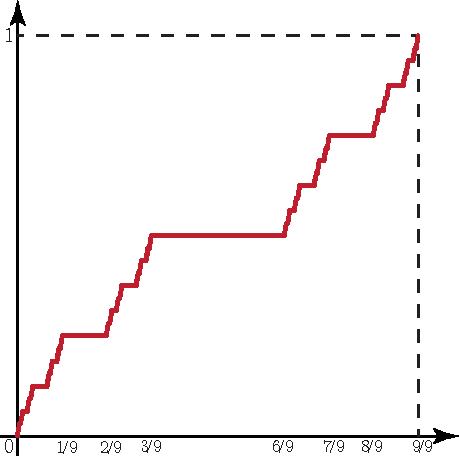
\includegraphics[width=0.4\paperwidth]{images/vasingolarecontinua}
\end{center}
Per quanto detto su tale funzione, essa soddisfa tutte le condizioni di essere la cdf di una variabile aleatoria singolarmente continua. In quanto tale, questa variabile aleatoria non ammette una funzione di densità, ma si può vedere, per simmetria.
\end{examplewt}
\subsection{Variabili aleatorie qualsiasi}
Abbiamo elencato tre diverse classi di misure di probabilità e variabili aleatorie ad esse associate. Il seguente teorema ci permette di affermare che esiste solo un'ulteriore classe di misure e variabili, le quali tuttavia non sono altro che combinazioni dei tre tipi precedentemente enunciati.
\begin{theoremaqed}[Teorema di Radon-Nikodym-Lebesgue]\index{teorema!di Radon-Nikodym-Lebesgue}
	Sia $\funz{\mathbb{P}}{\mathcal{B}\left(\realset\right)}{\left[0,1\right]}$ una misura di probabilità. Allora esistono $\alpha_1,\ \alpha_2,\ \alpha_3\geq 0$ e tre misure di probabilità $\mathbb{P}^{ac},\ \mathbb{P}^{sd},\ \mathbb{P}^{sc}$ assolutamente continua, singolare discreta e singolare continua, rispettivamente, tali che
	\begin{equation}
		\mathcal{P}=\alpha_1\mathbb{P}^{ac}+\alpha_2\mathbb{P}^{sd}+\alpha_3\mathbb{P}^{sc}\qedhere
	\end{equation}
\end{theoremaqed}
Come conseguenza, ogni variabile aleatoria si decompone nella somma di tre variabili aleatorie, una assolutamente continua, una discreta e una singolare continua.
\section{Modi di convergenza nella teoria della probabilità}
Come abbiamo potuto notare, la teoria assiomatica della probabilità è profondamente legata alla teoria della misura. Nella sezione \ref{modiconvergenza} abbiamo visto diversi modi in cui una successione di funzioni misurabili $\funz{f_n}{X}{\complexset}$ poteva convergere ad una funzione limite misurabile $\funz{f}{X}{\complexset}$. Studiamo ora i modi di convergenza di una successione di variabili aleatorie $\funz{X_n}{\Omega}{\complexset}$ ad una variabile aleatoria limite $\funz{X}{\Omega}{\complexset}$.
\paragraph{Convergenza puntuale o convergenza certa}
\begin{define}[Convergenza puntuale o convergenza certa]
	Consideriamo lo spazio di probabilità $\left(\Omega,\mathcal{F},\mathbb{P}\right)$ e le variabili aleatorie $\funz{X_n,X}{\Omega}{\complexset}$
	Si dice che $X_n$ \textbf{converge certamente}\index{convergenza!certa} a $X$\textbf{su} $\Omega$ ($X_n\overset{\text{c.}}{\to} X$) se
	\begin{equation}
		\lim_{n\to+\infty}X_n\left(\omega\right)=X\left(\omega\right),\ \forall \omega\in\Omega
	\end{equation}
\end{define}
La convergenza certa implica tutti i modi di convergenza successivi, ma \textit{non c'è alcun vantaggio} ad usare questa convergenza rispetto alla convergenza quasi certa.
\paragraph{Convergenza quasi certa}
\begin{define}[Convergenza quasi certa]
	Consideriamo lo spazio di probabilità $\left(\Omega,\mathcal{F},\mathbb{P}\right)$ e le variabili aleatorie $\funz{X_n,X}{\Omega}{\complexset}$
	Si dice che $X_n$ \textbf{converge quasi certamente}\index{convergenza!quasi certa} a $X$\textbf{su} $\Omega$ ($X_n\overset{\text{q.c.}}{\to} X$) se
	\begin{equation}
		\mathbb{P}\left(\left\{\omega\in\Omega \ \middle| \ \lim_{n\to+\infty}X_n\left(\omega\right)=X\left(\omega\right)\right\}\right)=1
	\end{equation}
\end{define}
Osserviamo che in uno spazio di probabilità $\left(\Omega,\mathcal{F},\mathbb{P}\right)$ questa convergenza è equivalente alla convergenza \textit{quasi ovunque}. Infatti:
\begin{align*}
	\left\{\omega\in \Omega\middle|\lim_{n\to+\infty}X_n\left(\omega\right)\neq X\left(\omega\right)\right\}&=\Omega\setminus\left\{\omega\in \Omega\middle|\lim_{n\to+\infty}X_n\left(\omega\right)= X\left(\omega\right)\right\}\\
	\mathbb{P}\left(\left\{\omega\in \Omega\middle|\lim_{n\to+\infty}X_n\left(\omega\right)\neq X\left(\omega\right)\right\}\right)&\underset{\mathbb{P}(x)<+\infty}{=}\mathbb{P}\left(\Omega\right)-\mathbb{P}\left(\left\{\omega\in \Omega\middle|\lim_{n\to+\infty}X_n\left(\omega\right)= X\left(\omega\right)\right\}\right)\\
	\mathbb{P}\left(\left\{\omega\in \Omega\middle|\lim_{n\to+\infty}X_n\left(\omega\right)\neq X\left(\omega\right)\right\}\right)&=1-\mathbb{P}\left(\left\{\omega\in \Omega\middle|\lim_{n\to+\infty}X_n\left(\omega\right)= X\left(\omega\right)\right\}\right)
\end{align*}
Allora affermare che
\begin{equation*}
	\mathbb{P}\left(\left\{\omega\in \Omega \ \middle| \ \lim_{n\to+\infty}X_n\left(\omega\right)= X\left(\omega\right)\right\}\right)=1
\end{equation*}
significa affermare che
\begin{equation*}
	\mathbb{P}\left(\left\{\omega\in \Omega \ \middle| \ \lim_{n\to+\infty}X_n\left(\omega\right)\neq X\left(\omega\right)\right\}\right)=0
\end{equation*}
\begin{attention}
	In uno spazio di misura che \textit{non} sia di probabilità questa corrispondenza non si può fare, dato che $\mu(X)$ può non essere pari ad $1$, tanto meno finito. Vale sempre la convergenza \textbf{q.o.}, ma mai quella \textbf{q.c.}.
\end{attention}
\newpage
\paragraph{Convergenza in probabilità}
\begin{define}[Convergenza in probabilità]
	Consideriamo lo spazio di probabilità $\left(\Omega,\mathcal{F},\mathbb{P}\right)$ e le variabili aleatorie $\funz{X_n,X}{\Omega}{\complexset}$. Si dice che	$X_n$ \textbf{converge in probabilità}\index{convergenza!in probabilità} a $X$ ($X_n\overset{\mathbb{P}}{\to} X$) se
	\begin{equation}
		\lim_{n\to+\infty}\mu\left(\left\{\omega\in \Omega\mid \abs{X_n\left(\omega\right)-X\left(\omega\right)}<\epsilon\right\}\right)=1,\ \forall \epsilon >0
	\end{equation}
\end{define}
In modo analogo alla convergenza quasi certa, in uno spazio di probabilità $\left(\Omega,\mathcal{F},\mathbb{P}\right)$ questa convergenza è equivalente alla \textit{convergenza in misura}.
\begin{attention}
	In uno spazio di misura che \textit{non} sia di probabilità questa corrispondenza non si può fare, dato che $\mu(X)$ può non essere pari ad $1$, tanto meno finito. Vale sempre la convergenza in misura, ma mai quella in probabilità.
\end{attention}
\paragraph{Convergenza in media}
\begin{define}[Convergenza in media]
	Consideriamo lo spazio di probabilità $\left(\Omega,\mathcal{F},\mathbb{P}\right)$ e le variabili aleatorie $\funz{X_n,X}{\Omega}{\complexset}$. Si dice che
	$X_n$ \textbf{converge in media}\index{convergenza!in media} a $f$ ($X_n\overset{L^1}{\to} X$) se
	\begin{equation}
		\lim_{n\to+\infty}\mathbb{E}X_n=\mathbb{E}X
	\end{equation}
	o, equivalentemente, se passiamo alla probabilità immagine,
	\begin{equation}
		\lim_{n\to+\infty}\int_\realset X_nd\mathbb{P}_Y=\int_{\realset}Xd\mathbb{P}_Y
	\end{equation}
\end{define}
\paragraph{Convergenza in legge}
\begin{define}[Convergenza in legge]
	Dato $\left(\Omega,\ \mathcal{M},\ \mathbb{P}\right)$ spazio di probabilità e le variabili aleatorie $\funz{X_n,\ X}{\Omega}{\realset}$ con le corrispettive \textit{funzioni di distribuzione}
	\begin{gather*}
		\funztot{F_n}{\realset}{\realset}{x}{F_n(x)=\mathbb{P}\left(X_n\leq x\right),\ \forall x\in \realset}\\
		\funztot{F}{\realset}{\realset}{x}{F(x)=\mathbb{P}\left(X\leq x\right),\ \forall x\in \realset}
	\end{gather*}
	allora si dice che $X_n$ converge a $X$ \textbf{in legge}\index{convergenza!in legge} $\left(X_n\stackrel{d}{\to}X\right)$ se
	\begin{equation}
		\lim_{n\to+\infty}F_n(x)=F(x),\ \forall x\in\realset\ \text{punto di continuità di }F.
	\end{equation}
\end{define}
\appendix
\part{Analisi forense del fatto di sangue}
\labelPart{appendix}
% SVN info for this file
\svnidlong
{$HeadURL$}
{$LastChangedDate$}
{$LastChangedRevision$}
{$LastChangedBy$}

\chapter{Note aggiuntive}
\labelAppendix{footnotes}
\addtocontents{define}{\noindent\textls{\textsc{\textcolor{reddo}{Appendice A:}
\nowtitle}}
}{}
\addtocontents{theorema}{\noindent\textls{\textsc{\textcolor{reddo}{Appendice A:}
			\nowtitle}}
}{}
\begin{introduction}
‘‘Le note a piè di pagina sono le superfici ingannatrici che permettono ai paragrafi tentacolari di aderire alla realtà più ampia della biblioteca.''
\begin{flushright}
	\textsc{Nicholson Baker,} bibliotecario di Cthulhu.
\end{flushright}
\end{introduction}

\noindent Riportiamo alcune note, precisazioni e dimostrazioni complementari agli argomenti dei capitoli principali che possono risultare utili al lettore.
\section{Capitolo 1: alla ricerca della lunghezza dell'ellisse}
\subsection{Il coefficiente binomiale generalizzato}\label{coefficientebinomialgeneralizzato}
\begin{define}[Coefficiente binomiale.]~{}\\
	Dati $n,j\in\naturalset$ con $n\geq j$, si definisce il \textbf{coefficiente binomiale}\index{coefficiente binomiale} il numero
	\begin{equation}
		\binom{n}{j}=\frac{n!}{j!\left(n-j\right)!}
	\end{equation}
dove $!$ indica il \textbf{fattoriale}\index{fattoriale}:
\begin{itemize}
	\item $\left(0\right)!=1$
	\item $\forall n\in\naturalset\quad n!=n\cdot \left(n-1\right)\cdot \ldots \cdot 3 \cdot 2 \cdot 1$
\end{itemize}
Se $n<j$, allora poniamo $\displaystyle\binom{n}{j}=0$
\end{define}
Possiamo estendere la definizione del coefficiente binomiale sostituendo a $n$ e $j$ dei qualunque numeri complessi $\alpha$ e $\beta$ (purché \textit{non} sia un intero negativo)  utilizzando la generalizzazione del fattoriale, la \textit{funzione Gamma di Eulero}. Vediamone la definizione con $\alpha$ tale che $\Re\left(\alpha\right)>0$.
\begin{define}[Funzione Gamma di Eulero.]~{}\\
	Dato $\alpha$ tale che $\Re\left(\alpha\right)>0$, definiamo la \textbf{funzione Gamma di Eulero}\index{funzione!Gamma di Eulero} in campo complesso come il prolungamento analitico dell'integrale improprio convergente
	\begin{equation}
		\Gamma\left(\alpha\right)=\int_{0}^{+\infty}x^{\alpha-1}e^{-\alpha}dx
	\end{equation}
	Essa gode di alcune proprietà:
	\begin{itemize}
		\item $\Gamma\left(1\right)=1$
		\item $\Gamma\left(\alpha+1\right)=\alpha\Gamma\left(\alpha\right),\ \forall\alpha>0$
		\item $\Gamma\left(n\right)=\left(n+1\right)!,\ \forall n\in\naturalset$
	\end{itemize}
\end{define}
Definita la funzione Gamma, diamo ora una definizione generalizzata di coefficiente binomiale.
\begin{define}[Coefficiente binomiale generalizzato con Gamma di Eulero.]~{}\\
	Dati $\alpha,\beta\in\complexset\setminus\left\{z\mid\Re\left(z\right)\in\integerset\wedge\Re\left(z\right)\leq0\right\}$, si definisce il \textbf{coefficiente binomiale generalizzato}\index{coefficiente binomiale!generalizzato} il numero
	\begin{equation}
		\binom{\alpha}{\beta}=\frac{\Gamma\left(\alpha+1\right)}{\Gamma\left(\beta+1\right)\Gamma\left(\alpha-j+1\right)}
	\end{equation}
\end{define}
Questa definizione è corretta, ma presenta alcuni inconvenienti:
\begin{itemize}
	\item \textit{Non è definita} sui complessi con parte reale un numero intero negativo o zero.
	\item \textit{Non è operativa}, dato che richiede di conoscere i valori della funzione Gamma che, in generale, non sono noti.
\end{itemize}
Consideriamo ora il caso del binomiale $\displaystyle\binom{\alpha}{j}$ dove $\alpha\in\complexset$ e $j\in\naturalset$. Se $\alpha\in\naturalset$, osserviamo come la forma operativa del binomiale è la seguente:
\begin{align*}
	\binom{\alpha}{j}&=\frac{\alpha!}{j!\left(\alpha-j\right)!}=\frac{\alpha\left(\alpha-1\right)\cdots\left(\alpha-j+1\right)\left(\alpha-j\right)\cdots 1}{j!\left(\alpha-j\right)!}=\frac{\alpha\left(\alpha-1\right)\cdots\left(\alpha-j+1\right)\Ccancel{\left(\alpha-j\right)!}}{j!\Ccancel{\left(\alpha-j\right)!}}\\
	&=\frac{\alpha\left(\alpha-1\right)\cdots\left(\alpha-j+1\right)}{j!}
\end{align*}
In realtà questa relazione si ottiene anche col coefficiente che abbiamo definito in precedenza se $\alpha\in\complexset$ e $j\in\naturalset$. Innanzitutto, diamo qualche notazione.
\begin{define}[Simbolo di Pochhammer o fattoriale crescente.]~{}\\
	Dati $\alpha\in\complexset$, $j\in\naturalset$, il \textbf{simbolo di Pochhammer}\seeonlyindex{fattoriale!crescente}{simbolo di Pochhammer} o altresì detto \textbf{fattoriale crescente}\index{fattoriale!crescente} è il numero
	\begin{equation}
		\alpha^{\overline{j}}=\left(\alpha\right)_j\coloneqq\frac{\Gamma\left(\alpha+j\right)}{\Gamma\left(\alpha\right)}
	\end{equation}
	Questa equivale a
	\begin{equation}
	\alpha^{\overline{j}}=\left(\alpha\right)_j=\prod_{k=0}^{j-1}\left(\alpha+j\right)=\prod_{k=1}^{j}\left(\alpha+j-1\right)=\alpha\left(\alpha+1\right)\cdots\left(\alpha+j-1\right)
\end{equation}
\end{define}
\begin{define}[Fattoriale decrescente.]~{}\\
	Dati $\alpha\in\complexset$, $j\in\naturalset$, il \textbf{fattoriale decrescente}\index{fattoriale!decrescente} è il numero
	\begin{equation}
		\alpha^{\underline{j}}\coloneqq\frac{\Gamma\left(\alpha+1\right)}{\Gamma\left(\alpha-j+1\right)}
	\end{equation}
	Questa equivale a
	\begin{equation}
	\alpha^{\underline{j}}=\prod_{k=0}^{j-1}\left(\alpha-j\right)=\prod_{k=1}^{j}\left(\alpha-j+1\right)=\alpha\left(\alpha-1\right)\cdots\left(\alpha-j+1\right)
\end{equation}
\end{define}
\begin{attention}
		La notazione $\left(\alpha\right)_j$, introdotta da Leo August Pochhammer, è talvolta usata anche per indicare il fattoriale \textit{decrescente} oltre che quello \textit{crescente}. Anche se useremo il simbolo di Pochammer solo per il fattoriale crescente, prediligeremo la notazione introdotta da Knuth et al. % TO DO: inserire riferimento bibliografico.
\end{attention}
Osserviamo che
\begin{equation*}
	\binom{\alpha}{j}=\frac{\Gamma\left(\alpha+1\right)}{j!\Gamma\left(\alpha-j+1\right)}=\frac{\alpha^{\underline{j}}}{j!}=\frac{\alpha\left(\alpha-1\right)\cdots\left(\alpha-j+1\right)}{j!}=\frac{\left(\alpha-j+1\right)^{\overline{j}}}{j!}=\frac{\left(\alpha-j+1\right)_j}{j!}
\end{equation*}
Allora possiamo considerare questa definizione operativa come la generalizzazione nel caso $\alpha\in\complexset$ e $j\in\naturalset$ del binomiale.
\begin{define}[Coefficiente binomiale generalizzato, definizione operativa.]~{}\\
	Dati $\alpha\in\complexset,\ j\in\naturalset$, si definisce il \textbf{coefficiente binomiale generalizzato}\index{coefficiente binomiale!generalizzato} il numero
	\begin{equation}
		\binom{\alpha}{j}=\frac{\alpha^{\underline{j}}}{j!}=\frac{\left(\alpha-j+1\right)^{\overline{j}}}{j!}=\frac{\left(\alpha-j+1\right)_j}{j!}=\frac{\alpha\left(\alpha-1\right)\cdots\left(\alpha-j+1\right)}{j!}
	\end{equation}
\end{define}
\begin{observe}
	Se $\alpha<j$, con $\alpha\in\integerset$ e $j\in\naturalset$, si ha al numeratore il fattore $\left(\alpha-\alpha\right)$ e quindi $\displaystyle\binom{\alpha}{j}=0$. Il 
\end{observe}
Valgono inoltre le seguenti proprietà, $\forall \alpha\in\complexset$:
\begin{align}
	&\binom{\alpha}{0}=1\\
	&\binom{\alpha}{k+1}=\binom{\alpha}{k}\frac{\alpha-k}{k+1}\\
	&\binom{\alpha}{k-1}+\binom{\alpha}{k}=\binom{\alpha+1}{k}
\end{align}
\section{Capitolo 3: serie di funzioni}
\subsection{Tanti criteri di Cauchy}\label{criteriodicauchy}
Il \textbf{criterio di Cauchy}\index{criterio!di Cauchy} è un importante teorema che fornisce condizioni necessarie e sufficienti per la convergenza di una successione.
\begin{theorema}[Criterio di Cauchy per le successioni.]~{}\\\index{criterio!di Cauchy!per le successioni}
		Sia $v_n$ successione in $X$ spazio metrico \textit{completo}. Allora
	\begin{multline}
		v_n\text{ converge in }X \iff v_n\text{ è di Cauchy}\iff\\
		\iff\forall \epsilon >0\ \exists N=N\left(\epsilon\right)\colon\forall n,m\geq N\ \mvf{d}{v_n}{v_m}<\epsilon
	\end{multline}
\end{theorema}
\begin{demonstration}~{}\\
	$\impliesdx$Supponiamo che $v_n$ converge a $v\in X$, ovvero
	\begin{equation*}
		\forall \epsilon>0\exists N=N\left(\epsilon\right)\colon\forall n\geq N\mvf{d}{v_n}{v}<\frac{\epsilon}{2}
	\end{equation*}
	Prendiamo $n,m\geq N$. Per la disuguaglianza triangolare della metrica $d$ si ha
	\begin{equation*}
		\mvf{d}{v_n}{v_m}<\mvf{d}{v_n}{v}+\mvf{d}{v}{v_m}=\mvf{d}{v_n}{v}+\mvf{d}{v_m}{v}<\frac{\epsilon}{2}+\frac{\epsilon}{2}=\epsilon
	\end{equation*}
	$\impliessx$Vale per la completezza dello spazio $X$.
\end{demonstration}
\begin{observe}
	L'implicazione $\impliesdx$vale in generale su qualunque spazio metrico, mentre l'altra vale solo se lo spazio è completo. Per dimostrare che $X$ sia completo può essere utile utilizzare alcune delle seguenti proprietà\footnote{Per approfondimenti si veda il Capitolo 6 di \cite{antucabertolotti:2021manualozzogeometria}.}:
	\begin{itemize}
		\item Una successione di Cauchy è \textit{convergente} se e solo se ha punti di accumulazione.
		\item Una successione di Cauchy è \textit{convergente} se ha una \textit{sottosuccessione convergente}.
		\item Se $X$ è spazio metrico \textit{compatto}, allora $X$ è spazio metrico \textit{completo}; non è vero il viceversa.
	\end{itemize}
\end{observe}
\begin{intuit}
	Possiamo vedere una successione di Cauchy come una successione che \textit{oscilla} sempre di meno, fino a posizionarsi su un valore relativamente costante, dove le oscillazioni fra due valori distinti della successione sono davvero piccole.
\end{intuit}
In termini matematici, possiamo formalizzare questa intuizione così: una oscillazione dopo l'$N$-esimo elemento è la più grande differenza fra due elementi della successione scelti arbitrariamente dopo l'$N$-esimo:
\begin{equation*}
	osc\left(N\right)\coloneqq\sup\left\{\mvf{d}{v_n}{v_m}\mid n,m\geq N\right\}
\end{equation*}
Allora una serie è di Cauchy se
\begin{equation*}
	\lim_{N\to+\infty}osc\left(N\right)=0
\end{equation*}
Questo ci permette di \textit{estendere} il criterio di Cauchy a situazione \textit{molto variegate} tra di loro dove bisogna studiare una convergenza, tutte \textit{accomunate} dall'idea che ‘‘portare l'oscillazione a \textit{zero} è equivalente alla convergenza''.\\
Abbiamo visto nel \refChapter{convergenzafunzioni}, a pag. \pageref{criteriodicauchyperconvergenzauniforme} il criterio di Cauchy per la \textit{convergenza uniforme}; qui di seguito riportiamo quello per le successioni.
\begin{corollary}[Criterio di Cauchy per le serie.]~{}\\\label{criteriodicauchyperleserie}\index{criterio!di Cauchy!per le serie}
	Una serie $\displaystyle\sum_{n=0}^{+\infty}x_n$ in uno spazio \textit{normato completo} è convergente se e solo se
	\begin{equation}
		\forall \epsilon>0\ \exists N\in\naturalset\colon\forall n\geq N,\ \forall p\in\naturalset\ \norm{x_{n+1}+x_{n+2}+\ldots+x_{n+p}}<\epsilon
	\end{equation}
\end{corollary}
\begin{demonstration}
	Considerate le ridotte $\displaystyle s_n=\sum_{k=1}^{n}a_k$, la serie $\displaystyle\sum_{n=0}^{+\infty}x_n$ converge se e solo se la successione delle ridotte converge. Poiché $X$ è uno spazio completo, questo equivale a dire che la successione delle ridotte $s_n$ è di Cauchy, ossia
	\begin{equation*}
		\forall \epsilon>0\ \exists N\in\naturalset\colon\forall n\geq N,\ \forall p\in\naturalset\ \norm{s_m-s_n}<\epsilon
	\end{equation*}
	Senza perdita di generalità poniamo $m=n+p$: la relazione qui sopra coincide con
	\begin{equation*}
		\forall \epsilon>0\ \exists N\in\naturalset\colon\forall n\geq N,\ \forall p\in\naturalset\ \norm{x_{n+1}+x_{n+2}+\ldots+x_{n+p}}<\epsilon
	\end{equation*}
	e quindi segue la tesi.
\end{demonstration}
% TO DO: continuare con altri criteri?
% TO DO: riportare qui le definizioni di successione di Cauchy, spazio normato
\subsection{Criteri di convergenza delle serie}\label{criteridiconvergenzaserie}
Di seguito enunceremo diversi criteri utili per studiare la convergenza di una serie $\displaystyle\sum_{n=1}^{+\infty}a_n$.
\begin{itemize}
	\item \textbf{Limite del termine della successione.} (\textit{Criterio necessario}, $\realset$ o $\complexset$) Se la serie converge, allora $\displaystyle\lim_{n\to+\infty}a_n=0$. Per contronominale vale
	\begin{equation}
		\lim_{n\to+\infty}a_n\neq 0\implies\sum_{n=1}^{+\infty}a_n\text{ non converge}
	\end{equation}
	\item \textbf{Convergenza assoluta.} (\textit{Criterio sufficiente}, $\realset$ o $\complexset$) Se la serie $\displaystyle\sum_{n=1}^{+\infty}\abs{a_n}$ converge, allora si dice che la serie $\displaystyle\sum_{n=1}^{+\infty}a_n$ converge \textit{assolutamente} e inoltre essa converge anche semplicemente.
	\item \textbf{Criterio del rapporto o di d'Alembert.} (\textit{Criterio sufficiente}, $\realset$ o $\complexset$)
	% Sia $a_n$ definitivamente diverso da zero.
	Se esiste $R$ tale che
	\begin{equation}
		\lim_{n\to+\infty}\abs{\frac{a_{n+1}}{a_n}}=R
	\end{equation}
	se $R<1$, la serie è \textit{assolutamente} convergente. Se $R>1$, la serie diverge. Se $R=1$, non abbiamo informazioni sulla convergenza.
	\item \textbf{Criterio della radice o di Cauchy.} (\textit{Criterio sufficiente}, $\realset$ o $\complexset$) Sia
	\begin{equation*}
		R = \limsup_{n\to+\infty}\sqrt[n]{\abs{a_n}}
	\end{equation*}
	se $R<1$, la serie è \textit{assolutamente} convergente. Se $R>1$, la serie diverge. Se $R=1$, non abbiamo informazioni sulla convergenza.\\
	Se una serie infinita converge o diverge col criterio della radice, lo stesso risultato si ottiene con il criterio del rapporto ma non vale il viceversa.
	\item \textbf{Criterio dell'integrale.} (\textit{Criterio necessario e sufficiente}, $\realset$) Sia $\funz{f}{\left[1,+\infty\right)}{\realset_+}$ una funzione non-negativa e monotona decrescente tale per cui $f\left(n\right)=a_n$. Allora, posto
	\begin{equation*}
		\int_{1}^{+\infty}f\left(x\right)dx=\lim_{t\to\infty}\int_{1}^{t}f\left(x\right)dx
	\end{equation*}
	la serie $a_n$ converge se e solo se l'integrale converge.
	\item \textbf{Criterio di confronto diretto.} (\textit{Criterio sufficiente}, $\realset$ o $\complexset$) Se la serie $\displaystyle\sum_{n=1}^{+\infty}b_n$ è una serie \textit{assolutamente} convergente e $\abs{a_n}<\abs{b_n}$ per $n$ sufficientemente largo, allora la serie $\displaystyle\sum_{n=1}^{+\infty}a_n$ converge \textit{assolutamente}.
	\item \textbf{Criterio del confronto asintotico} (\textit{Criterio necessario e sufficiente}, $\realset$) Se $a_n,\ b_n>0,\ \forall n$, e il limite $\displaystyle\lim_{n\to+\infty}\frac{a_n}{b_n}$ esiste, è finito e diverso da zero, allora
	\begin{center}
		$\displaystyle\sum_{n=1}^{+\infty}a_n$ converge $\displaystyle\iff\sum_{n=1}^{+\infty}b_n$ converge.
	\end{center}
	\item \textbf{Criterio di condensazione di Cauchy.} (\textit{Criterio necessario e sufficiente}, $\realset$) Sia $a_n$ una successione non negativa e non crescente. Allora
	\begin{center}
		$\displaystyle\sum_{n=1}^{+\infty}a_n$ converge $\displaystyle\iff\sum_{n=1}^{+\infty}2^na_{2^n}$ converge.
	\end{center}
	Inoltre, nel caso di convergenza, si ha
	\begin{equation*}
		\sum_{n=1}^{+\infty}a_n<\sum_{n=1}^{+\infty}2^na_{2^n}<2\sum_{n=1}^{+\infty}a_n
	\end{equation*}
	\item \textbf{Criterio di Abel-Dirichlet.} (\textit{Criterio sufficiente}, $\realset$ o $\complexset$) Sia data la serie
	\begin{equation}
		\sum_{n=0}^{+\infty}a_nb_n,\quad a_n\in\complexset,\ b_n\in\realset
	\end{equation}
	Se
	\begin{itemize}
		\item $b_n>0$ è decrescente e infinitesima per $n\to+\infty$.
		\item la successione delle somme parziali di $a_n$ è limitata, ossia
		\begin{equation*}
			\exists M>0\colon\abs{\sum_{k=0}^{n}a_k}\leq M,\ \forall k\leq 0
		\end{equation*}
	\end{itemize}
	allora la serie $\displaystyle\sum_{n=0}^{+\infty}a_nb_n$ converge (semplicemente).
	\item \textbf{Criterio di Leibniz.} (\textit{Criterio sufficiente}, $\realset$ o $\complexset$) Sia data la serie
		\begin{equation}
		\sum_{n=0}^{+\infty}\left(-1\right)^na_n,\quad a_n\in\realset
	\end{equation}
	Se $a_n>0$ è decrescente ed infinitesima per $n\to+\infty$, allora la serie $\displaystyle\sum_{n=0}^{+\infty}\left(-1\right)^na_n$ converge (semplicemente).
\end{itemize}
\subsection{Serie a valori reali notevoli}\ref{serieavalorirealinotevoli}
Di seguito enunceremo alcune serie a valori reali di particolare rilevanza.
\begin{itemize}
	\item \textbf{Serie geometrica.}
	\begin{equation*}
		\sum_{n=0}^{+\infty}z^{n}
	\end{equation*}	
	La ridotta è uguale a
	\begin{equation*}
		s_n=\sum_{k=0}^{n}z^{k}=\frac{1-z^{n+1}}{1-z}
	\end{equation*}
	La serie dunque converge se e solo se $\abs{z}<1$ e in tal caso converge a $\displaystyle\frac{1}{1-z}$.
	\item \textbf{Serie armonica generalizzata.}
	\begin{equation}
		\sum_{n=1}^{+\infty}\frac{1}{n^p}
	\end{equation}
	converge se $p>1$ e diverge per $p\leq 1$; per $p=1$ abbiamo la \textbf{serie armonica}. Se $p>1$ la somma della serie armonica generalizzata, se vista in funzione di $p$, è  $\zeta\left(p\right)$, ossia la \textit{funzione zeta di Riemann} valutata in $p$.
	\item \textbf{Serie logaritmica.}
	\begin{equation}
		\sum_{n=2}^{+\infty}\frac{1}{n\left(\log n\right)^p}
	\end{equation}
	per ogni numero reale positiva $p$. Diverge per $p\leq 1$, ma converge per ogni $p>1$.
\end{itemize}
\section{Capitolo 4: serie di potenze}
\subsection{Il prodotto di serie (secondo Cauchy)}\label{prodottosecondocauchy}
In questa sezioni ricordiamo la definizione ed alcune proprietà del prodotto di serie (secondo Cauchy), basandoci sul Capitolo 3 di \cite{rudin:1976principles}.\\
Date le due serie
\begin{equation*}
	\sum_{n=0}^{+\infty} \alpha_n,\quad \sum_{n=0}^{+\infty} \beta_n,\quad \alpha_n, \ \beta_n \in \complexset
\end{equation*}
vogliamo definire il loro prodotto. L'idea alla base della definizione è quella di \textit{generalizzare} il prodotto di due \textit{polinomi}: è noto che, dati i polinomi 
\begin{equation*}
	\sum_{n=0}^{J} \alpha_n z^n,\quad \sum_{n=0}^{J} \beta_n z^n
\end{equation*}
il loro prodotto si scrive come
\begin{equation*}
	\sum_{n=0}^{2J} \gamma_n z^n\quad\text{con}\quad\gamma_n= \sum_{k=0}^{n} \alpha_k\beta_{n-k},\quad \forall \ n\geq 0
\end{equation*}
Possiamo estendere formalmente questa scrittura al caso di serie di potenze, ponendo
\begin{equation*}
	\sum_{n=0}^{+\infty} \alpha_n z^n \cdot \sum_{n=0}^{+\infty} \beta_n z^n = \sum_{n=0}^{+\infty} \gamma_n z^n
\end{equation*}
dove $\gamma_n$ è definito come precedentemente. Il risultato per $z=1$ suggerisce quindi come definire il prodotto delle serie iniziali.
\begin{define}[Prodotto di serie {(secondo Cauchy)}.]~{}\\
	Date le serie
	\begin{equation*}
		\sum_{n=0}^{+\infty} \alpha_n,\quad \sum_{n=0}^{+\infty} \beta_n,\quad \alpha_n, \ \beta_n \in \complexset
	\end{equation*}
si definisce \textbf{prodotto secondo Cauchy}\index{prodotto!secondo Cauchy} la serie
\begin{equation*}
	\sum_{n=0}^{+\infty} \gamma_n\quad\text{con}\quad\gamma_n= \sum_{k=0}^{n} \alpha_k\beta_{n-k},\quad \forall \ n\geq 0
\end{equation*}
\end{define}
Il problema principale sul prodotto di serie è quello della sua convergenza, a partire dalla convergenza delle serie iniziali: più precisamente, ci si chiede:
\begin{center}
	se le serie iniziali convergono rispettivamente a $\alpha$ e $\beta$, la serie prodotto converge a $\alpha\beta$?
\end{center}
In generale la risposta è \textbf{no}, come mostra il prossimo esempio.
\begin{example}\textsc{Serie convergenti, aventi prodotto non convergente.}\\
	Consideriamo la serie
	\begin{equation*}
		\sum_{n=0}^{+\infty} \frac{(-1)^n}{\sqrt{n+1}}
	\end{equation*}
	Applicando il criterio di Leibniz, si verifica facilmente che la serie converge. La serie prodotto della serie data per se stessa ha termine generale
	\begin{equation*}
		\gamma_n = \sum_{k=0}^n \frac{(-1)^k}{\sqrt{k+1}}\, \frac{(-1)^{n-k}}{\sqrt{n-k+1}} = (-1)^n \, \sum_{k=0}^n \frac{1}{\sqrt{(n-k+1)(k+1)}},\quad \forall \ n\geq 0.
	\end{equation*}
	Ora, si ha
	\begin{equation*}
		(n-k+1)(k+1)=\left(\frac{n}{2}+1\right)^2- \left(\frac{n}{2}-k\right)^2\leq \left(\frac{n}{2}+1\right)^2=\left(\frac{n+2}{2}\right)^2,\ \forall n\geq 0, \ 0\leq k\leq n
	\end{equation*}
	 Otteniamo quindi
	 \begin{equation*}
	 	\abs{\gamma_n}= \sum_{k=0}^n \frac{1}{\sqrt{(n-k+1)(k+1)}}\geq  \sum_{k=0}^n \frac{2}{n+2}=\frac{2(n+1)}{n+2},\quad \forall \ n\geq 0.
	 \end{equation*}
	 Questo prova che 
 \begin{equation*}
 	\liminf_{n\to +\infty} \abs{\gamma_n}\geq \liminf_{n\to +\infty} \frac{2(n+1)}{n+2} = 2\implies \lim_{n\to +\infty} \abs{\gamma_n}\neq 0.
 \end{equation*}
Perciò si ha
\begin{equation*}
	\lim_{n\to +\infty} \gamma_n \neq 0
\end{equation*}
e quindi la serie prodotto non può convergere.
\end{example}
Osserviamo che nell'esempio riportato la serie iniziale \textit{converge semplicemente}, ma non \textit{assolutamente}; questo è il motivo per cui la serie prodotto \textit{non converge}. Infatti, in presenza della convergenza assoluta la serie prodotto \textit{converge}.
\begin{theorema}[Prodotto di serie {(secondo Cauchy)} convergente se una serie converge assolutamente.]~{}\\
	Siano date le due serie 
	\begin{equation*}
		\sum_{n=0}^{+\infty} \alpha_n,\quad \sum_{n=0}^{+\infty} \beta_n,\quad \alpha_n, \ \beta_n \in \complexset,
	\end{equation*}
	e si supponga che esse convergano a $\alpha$ e $\beta$, rispettivamente. 
	Inoltre, si supponga che \textit{almeno una} di esse converga \textit{assolutamente}.
	Allora, la loro serie prodotto converge a $\alpha \beta$.
\end{theorema}
\section{Capitolo 5: teoria della misura}
\subsection{Brevi cenni di teoria degli insiemi}
% TO DO: aggiungere biblio ref a Jech, Set Theory
% TO DO: spostare in un altro capitolo?
Questa sezione è basata sul capitolo 3 di XXX.\\
\paragraph{Teoria degli insiemi di Zermelo-Fraenkel e Assioma di Scelta}
% TO DO: add axiom environment
% TO DO: add proprietà environment
\paragraph{Insiemi ben ordinati}
% TO DO: aggiungere  def. ben ordinato
\paragraph{Ordinali}
\paragraph{Cardinalità}
Definiremo la cardinalità per insiemi \textit{ben ordinati}; poiché per l'\textit{Assioma di Scelta} ogni insieme è ben ordinato, la seguente definizione risulta essere valida sotto la teoria degli insiemi di \textbf{Zermelo–Fraenkel} con l'Assioma di Scelta ($\mathsf{ZFC}$).
\begin{define}[Cardinalità.]~{}\\
	Due insiemi $X$ e $Y$ hanno la stessa \textbf{cardinalità}\index{cardinalità} se sono \textbf{equipotenti}\index{equipotenza} o \textbf{equinumerosi}\seeonlyindex{equipotenza}{equinumerosità}, ossia se esiste una corrispondenza \textit{biunivoca} tra i due insiemi. Tale relazione si indica come
		\begin{equation}
		\abs{X}=\abs{Y}
	\end{equation}
\end{define}
L'equipotenza è una relazione di equivalenza sulle classi di tutti gli insiemi. Ad ogni insieme $X$ possiamo assumere di associare il \textbf{numero cardinale}\seeonlyindex{numero!cardinale}{cardinalità} o \textbf{cardinale}\seeonlyindex{cardinale}{cardinalità} $\abs{X}$, in modo tale che due insiemi che hanno lo stesso numero cardinale soddisfino la condizione di equipotenza.
\begin{digression}
	Se consideriamo valido l'\textit{Assioma di Regolarità} è comunque possibile definire la cardinalità anche senza l'\textit{Assioma di Scelta} sulla base delle relazioni di equivalenza indotte dall'equipotenza.
\end{digression}
Ricordiamo che $X$ è \textit{finito} se è in corrispondenza biunivoca con un \textit{ordinale finito} $n\in\naturalset$:
\begin{equation*}
	\abs{X}=\abs{n}
\end{equation*}
Poichè $\abs{n}=\abs{m}\iff n=m$, gli \textit{ordinali finiti} corrispondono ai \textit{cardinali finiti} e quindi $\abs{n}=n$, ossia
\begin{equation*}
	\abs{X}=n
\end{equation*}
Denotiamo ora alcuni cardinali \textit{infiniti} che appaiono frequentemente:
\begin{itemize}
	\item $\abs{\naturalset}=\aleph_{0}$: \textbf{cardinalità dei naturali}\index{cardinalità!dei naturali} o \textbf{cardinalità degli insiemi infinitamente numerabili} (si legge ‘‘\textit{aleph zero}'').
	\item $\abs{\realset}=\mathfrak{c}$: \textbf{cardinalità dei reali} o \textbf{cardinalità del continuo}\index{cardinalità!del continuo}.
\end{itemize}
\paragraph{Ordine dei cardinali}
Possiamo definire una relazione d'\textit{ordine} sui cardinali come segue:
\begin{equation}
	\abs{X}\leq \abs{Y}\iff \exists \funz{f}{X}{Y}\text{ iniettiva}
\end{equation}
Inoltre, definiamo l'ordine stretto
\begin{equation}
	\abs{X}<\abs{Y}\iff \abs{X}\leq \abs{Y}\wedge \abs{X}\neq\abs{Y}
\end{equation}
ossia se
\begin{itemize}
	\item esiste una funzione $\funz{f}{X}{Y}$ iniettiva.
	\item non esistono funzioni $\funz{f}{X}{Y}$ suriettive.
\end{itemize}
Sulla base di queste definizioni possiamo enunciare già una serie di proprietà interessanti che collegano questa relazione d'ordine alle ben note \textit{relazioni insiemistiche} di inclusione e uguaglianza di insiemi.
\begin{proposition}[Relazioni insiemistiche e ordine delle cardinalità.]~{}\\\label{cardinalitàugualenonimplicauguaglianzainsiemistica}
Dati $X$ e $Y$ insiemi:
\begin{itemize}
		\item $X\subseteq Y\iff \exists \incl{\iota}{X}{Y}$ inclusione $\iff \abs{X}\leq \abs{Y}$.
		\item $X\supseteq Y\iff \exists \funz{f}{X}{Y}$ suriettiva $\iff \abs{X}\geq \abs{Y}$. % TO DO: controllare se è vero effettivamente
		\item Se $\abs{X}<\abs{Y}$, allora $X\supsetneqq Y$.
		\item Se $X$ e $Y$ sono \textit{finiti}, allora $\abs{X}=\abs{Y}\iff X=Y$; se $X$ e $Y$ sono \textit{infiniti} $\abs{X}=\abs{Y}\Ccancel[black]{\implies}X=Y$ - vale soltanto la relazione banale $X=Y\implies \abs{X}=\abs{Y}$. % TO DO: aggiungere commento su questi risultati?
\end{itemize}
\end{proposition}
Il seguente teorema è particolarmente importante: oltre ad avere come conseguenza che $<$ è una relazione d'ordine \textit{parziale}, permette di determinare alcune cardinalità sulla base di sole funzioni \textit{iniettive}.
\begin{theorema}[Cantor-Bernstein-Schröder.]~{}\\
	Se $\abs{X}\leq\abs{Y}$ e $\abs{Y}\leq\abs{X}$, allora $\abs{X}=\abs{Y}$.\\
	Equivalentemente, se esistono due funzioni \textit{iniettive} $\funz{f}{X}{Y}$ e $\funz{g}{Y}{X}$ allora esiste una funzione \textit{biettiva} $\funz{h}{X}{Y}$.
\end{theorema}
\begin{examples}\textsc{Alcune applicazioni del teorema di Cantor-Bernstein-Schröder.}~{}
	\item L'intervallo $\left[0,1\right]$ ha la cardinalità del continuo; infatti, possiamo considerare le seguenti funzioni iniettive
	\begin{itemize}
		\item $\incl{\iota}{\left[0,1\right]}{\realset}$ inclusione.
		\item $\funztot{f}{\realset}{\left[0,1\right]}{x}{\frac{2\left(\arctan\left(x\right)+\frac{\pi}{2}\right)}{\pi}}$
	\end{itemize}
	\item Come visto a pag. XXX, dato l'insieme di Cantor $C$ si può definire una funzione $\funz{f}{C}{\left[0,1\right]}$ \textit{suriettiva}; in questo modo, $\abs{C}\geq \left[0,1\right]$ ma, in quanto $C\subseteq \left[0,1\right]$ si ha $\abs{C}=\abs{\left[0,1\right]}=\mathfrak{c}$. % TO DO: aggiunge pagina su Cantor o nelle note aggiuntive oppure nel libro in sè
\end{examples}
\paragraph{Aritmetica dei cardinali}
Possiamo definire delle \textit{operazioni aritmetiche} con i cardinali; dati $\abs{X}=\kappa$ e $\abs{Y}=\lambda$, si ha
\begin{align}
	\kappa+\lambda=\abs{X\cup Y}&\text{ se }X\text{ e }Y\text{ disgiunti}\\
	\kappa\cdot\lambda\abs{X\times Y}&\\
	\kappa^{\lambda}=\abs{X^Y}
\end{align}
dove con $X^Y$ indichiamo l'insieme delle funzioni da $Y$ in $X$.\\
Queste operazioni sono ben definite se sono indipendenti dalla scelta di $X$ e $Y$.
\paragraph{Cardinalità dell'insieme delle parti}
\begin{theorema}[Biezione tra {$\setpart{X}$} e insieme delle funzioni da {$X$} in {$\{0,1\}$}.]~{}\\
	Dato un qualunque insieme $X$, sia $\setpart{X}$ l'insieme delle parti di $X$ e sia $2^X\coloneqq\left\{0,1\right\}^X$ l'insieme di tutte le funzioni $\funz{\ }{X}{\left\{0,1\right\}}$. Allora esiste una biezione tra $\setpart{X}$ e $2^X$, data da
	\begin{equation}
		\funztot{\Phi}{\setpart{X}}{2^X}{X}{\chi_X}
	\end{equation}
	con $\chi_X$ la \textit{funzione indicatrice} su $X$; l'inversa di tale funzione è la seguente:
	\begin{equation}
		\funztot{\Phi^{-1}}{2^X}{\setpart{X}}{f}{\left\{x\in\ X\mid f\left(x\right)=1\right\}}
	\end{equation}
\end{theorema}
\begin{corollary}[Cardinalità dell'insieme delle parti.]~{}\\
	Se un insieme $X$ ha cardinalità $\abs{X}$, l'insieme delle parti ha cardinalità
	\begin{equation}
		\abs{\setpart{X}}=2^{\abs{X}}
	\end{equation}
\end{corollary}
\begin{demonstration}
	Per il teorema precedente, si ha una biezione tra $\setpart{X}$ e $2^{\abs{X}}\coloneqq\left\{0,1\right\}^{X}$, dunque hanno la stessa cardinalità. Per esponenziazione dei cardinali, si ha
	\begin{equation*}
		\abs{\setpart{X}}=\abs{\{0,1\right\}^{X}}=\abs{\{0,1\right\}}^{\abs{X}}=2^{\abs{X}}
	\end{equation*}
\end{demonstration}
Poiché questo corollario vale sia per insiemi arbitrari, l'immediata conseguenza del corollario è poter definire la cardinalità dell'insieme delle parti di insiemi \textit{infiniti} già noti:
\begin{itemize}\label{cardinalitàinsiemepartiinfiniti}
	\item $\abs{\setpart{\naturalset}}=2^{\aleph_{0}}$
	\item $\abs{\setpart{\realset}}=2^{\mathfrak{c}}$
\end{itemize}
Il seguente teorema permette di dare una relazione di ordine \textit{non} triviale tra cardinali.
\begin{theorema}[Cantor.]~{}\\
	Per ogni insieme $\abs{X}$ si ha
	\begin{equation}
		\abs{X}<\abs{\setpart{X}}
	\end{equation}
	In termini di cardinali, per ogni cardinale $\kappa$ si ha
	\begin{equation}
		\kappa < 2^{\kappa}
	\end{equation}
\end{theorema}
\subsection{Famiglie di insiemi e relazioni tra di loro}
Studiamo ora alcune delle più comuni \textit{famiglie di insiemi} che si incontrano nello studio della teoria della misura.
\begin{center}
	\begin{tabular}{c|c|c}
	\textbf{Nome}                                                                            & \textbf{Notazione}                          & \textbf{Cardinalità}        \\ \hline
	Insieme delle parti                                                             & $\setpart{\realset}$               & $2^{\mathfrak{c}}$ \\ \hline
	\begin{tabular}[c]{@{}c@{}}Insiemi misurabili\\ (secondo Lebesgue)\end{tabular} & $\mathcal{L}\left(\realset\right)$ & $2^{\mathfrak{c}}$ \\ \hline
	Borelliani                                                                      & $\mathcal{B}\left(\realset\right)$ & $\mathfrak{c}$     \\ \hline
	\begin{tabular}[c]{@{}c@{}}Topologia\\ (famiglia degli aperti)\end{tabular}     & $\topo$                            & $\mathfrak{c}$    
\end{tabular}
\end{center}
\begin{proposition}[Relazioni tra classi di insiemi.]~{}\\
	Valgono le seguenti inclusioni:
	\begin{equation}
		\topo\subsetneqq\mathcal{B}\left(\realset\right)\subsetneqq\mathcal{L}\left(\realset\right)\subsetneqq\setpart{\realset}
	\end{equation}
\end{proposition}
Mostreremo alcune di queste inclusioni in modo formale, mentre per altre daremo solo un'intuizione della dimostrazione.
\paragraph{Cardinalità dell'insieme delle parti dei reali}
Come visto a pag. \pageref{cardinalitàinsiemepartiinfiniti}, se $\abs{\realset}=\mathfrak{c}$ è la cardinalità del continuo, allora la cardinalità dell'\textit{insieme delle parti dei reali} è
\begin{equation}
	\abs{\setpart{\realset}}=2^{\mathfrak{c}}
\end{equation}
\paragraph{Cardinalità degli insiemi misurabili}
Per trovare quanti sono gli insiemi misurabili, consideriamo l'\textit{insieme di Cantor} $C$. Abbiamo visto (pag. XXX) che esso gode delle seguenti proprietà: % TO DO: aggiunge pagina su Cantor o nelle note aggiuntive oppure nel libro in sè
\begin{enumerate}
	\item Il numero di punti prima e dopo il processo iterativo per costruire $C$ rimane invariato, dunque $C$ è \textit{non numerabile} e ha la stessa cardinalità di $\left[0,1\right]$:
	\begin{equation*}
		\abs{C}=\abs{\left[0,1\right]}=\mathfrak{c}
	\end{equation*}
	\item $C$ è misurabile e $m_1\left(C\right)=0$.
\end{enumerate}
Dal punto 1 segue che l'insieme delle parti dell'insieme di Cantor ha cardinalità $\setpart{C}=2^{\mathfrak{c}}$, mentre dal punto 2 si può dedurre che ogni sottoinsieme di $C$ ha misura nulla ed è pertanto misurabile. Insiemisticamente parlando, le relazioni sono
\begin{equation*}
	\setpart{C}\subseteq \mathcal{L}\left(\realset\right)\subseteq\setpart{\realset}
\end{equation*}
Passando alle cardinalità:
\begin{equation*}
	2^{\mathfrak{c}}\underset{(1)}{\abs{\setpart{C}}}\leq \abs{\mathcal{L}\left(\realset\right)}\leq\abs{\setpart{\realset}}=2^{\mathfrak{c}}\implies \abs{\mathcal{\realset}}=2^{\mathfrak{c}}
\end{equation*}
\paragraph{Inclusione stretta di {$\mathcal{L}\left(\realset\right)$} in  {$\setpart{\realset}$}}
Il fatto che la cardinalità degli insiemi Lebesgue-misurabili in $\realset$ coincida con quella dell'insieme delle parti di $\realset$ non è sufficiente\footnote{Si veda pag. \pageref{cardinalitàugualenonimplicauguaglianzainsiemistica}.} per affermare che i due insiemi coincidano; costruiamo ora un sottoinsieme particolare di $\realset$ che risulta \textit{non misurabile}.\\
\begin{define}[Insieme di Vitali.]~{}\\
	Considerata in $\realset$ la relazione di equivalenza
	\begin{equation}
		x\sim y\iff x-y\in\rationalset
	\end{equation}
	possiamo definire delle classi di equivalenza in $\nicefrac{\realset}{\sim}$:
	\begin{align*}
		\left[0\right]=\left\{0,1,\frac{1}{2},-\frac{3}{4},\frac{123}{72},\ldots\right\}=\left\{x\in\realset\mid x\in\rationalset\right\}=\rationalset\\
		\left[\sqrt{2}\right]=\left\{\sqrt{2},\sqrt{2}+\frac{1}{2},\sqrt{2}-1,\ldots\right\}=\left\{x\in\realset\mid x=\sqrt{2}+q,\ q\in\rationalset\right\}\\
		\left[\pi\right]=\left\{\pi,\pi-\frac{3}{4},\pi+23,\ldots\right\}=\left\{x\in\realset\mid x=\pi+q,\ q\in\rationalset\right\}\\
		\vdots
	\end{align*}
	Scelto\footnote{Per poter fare questa operazione è necessario supporre l'\textit{Assioma di Scelta}.} un elemento che stia in $\left[0,1\right]$ da ogni classe di equivalenza, definisco l'\textbf{insieme di Vitali}\index{insieme!di Vitali} $V$ come unione di questi elementi.
\end{define}
Per costruzione $V\subseteq\left[0,1\right]$. Preso l'insieme \textit{numerabile} $\rationalset\cap\left[0,1\right]$, possiamo prendere una sua \textit{numerazione} $\left\{q_n\right\}$ e definire delle \textit{traslazioni} dell'insieme di Vitali $V$:
\begin{equation*}
	V_n=V+q_n\subseteq\left[-1,2\right]
\end{equation*}
\begin{lemming}[Gli insiemi di Vitali traslati sono 2 a 2 disgiunti.]
	Dato $V$ insieme di Vitali e $\left\{q_n\right\}$ numerazione di $\rationalset\cap\left[0,1\right]$, allora $V_n\cap V_m=\emptyset,\ \forall n\neq m$.
\end{lemming}
\begin{demonstration}
	Supponiamo
\end{demonstration}
% SVN info for this file
\svnidlong
{$HeadURL$}
{$LastChangedDate$}
{$LastChangedRevision$}
{$LastChangedBy$}

\chapter{Brevi cenni di Teoria degli Insiemi}
\labelAppendix{settheory}
\addtocontents{define}{\noindent\textls{\textsc{\textcolor{reddo}{Appendice B:}
\nowtitle}}
}{}
\addtocontents{theorema}{\noindent\textls{\textsc{\textcolor{reddo}{Appendice B:}
			\nowtitle}}
}{}
\begin{introduction}
‘‘La Logica è l'arte di sbagliare con confidenza.''
\begin{flushright}
	\textsc{Morris Kline,} commentando questo capitolo.
\end{flushright}
\end{introduction}
\lettrine[findent=1pt, nindent=0pt]{Q}{uando} nella vita di tutti i giorni utilizziamo i numeri naturali, lo facciamo con due scopi ben precisi:
\begin{itemize}
	\item \textbf{Contare} quanti oggetti ci sono in un insieme, associando una \textit{dimensione} ad esso: ‘‘Ci sono \textit{tre} mele nel cestino''.
	\item \textbf{Ordinare} un insieme di oggetti, ossia formare una sequenza assegnando un \textit{indice} ad ogni elemento dell'insieme: ‘‘Torino è la \textit{quarta} città italiana per numero di abitanti''.
\end{itemize}
\parshape=0
Per insiemi \textit{finiti}, non c'è apparente differenza tra i due concetti. Osserviamo che il numero di naturali (compreso lo zero) prima della $n$-esima posizione sono $n$, dunque in una sequenza di elementi indicizzata da $0$ con ultimo indice $n$ si hanno $n+1$ elementi. In altre parole, ordinando gli elementi è possibile sapere quanti sono e viceversa.\\
Questa due nozioni, come vedremo, divergono non appena generalizziamo i due concetti di ‘‘contare'' e ‘‘ordinare'' agli insiemi infiniti: ci sono molteplici ordinali infiniti che corrispondono allo stesso cardinale; inoltre, sotto certe ipotesi, potrebbero esserci insiemi che ammettono cardinalità ma che \textit{non} ammettono ordinali!\\
Lo scopo di questo capitolo aggiuntivo è cercare di dare alcune basi di \textbf{teoria degli insiemi} e \textbf{teoria degli ordini}, con il preciso scopo di spiegare come si ‘‘conta'' e si ‘‘ordina'' su insiemi infiniti.\\
Dopo una premessa sugli \textit{assiomi} sui quali baseremo i nostri ragionamenti, partiremo dal definire \textit{insiemi (ben) ordinati}, necessari per introdurre gli \textit{ordinali} (finiti e infiniti); arriveremo a parlare dell'\textit{induzione transfinita} e dell'aritmetica degli ordinali.\\
Successivamente, passeremo ai concetti di \textit{cardinalità} e \textit{numeri cardinali}, mostrando diverse proprietà (compreso lo stretto legame che li lega agli ordinali), concludendo con alcuni importanti teoremi e congetture.\\
Per maggiori approfondimenti rimandiamo a \cite{jech:2003settheory} e \cite{andretta:2021elements}.
%NOTA: la citazione deve apparire così a schermo? perché è letteralmente quanto scritto nel \cite, solo che è in grassetto e non è clickabile
\section{Teoria degli insiemi di Zermelo-Fraenkel e Assioma di Scelta}
Intuitivamente, un \textit{insieme} è una collezione di tutti gli elementi che soddisfano una certa proprietà. Potremmo dunque definire il seguente assioma...
\begin{falseaxiom}[Assioma della comprensione]
	Se $P$ è una proprietà, allora esiste un insieme degli elementi che soddisfano tale proprietà:
	\begin{equation*}
		Y=\left\{x \ \middle| \ P\left(x\right)\right\}
	\end{equation*}
\end{falseaxiom}
... che è però \textbf{falso} per il famoso \textbf{Paradosso di Russell}.
\begin{examplewt}[Paradosso di Russell]
	Si consideri l'insieme $S$ i cui elementi sono tutti e soli gli insiemi che non sono elementi di loro stessi:
	\begin{equation*}
		S=\left\{X \ \middle| \ X\notin X\right\}
	\end{equation*}
L'insieme $S$ appartiene a $S$? Se $S$ appartiene a $S$, allora $S$ non è un elemento di se stesso e quindi si ha $S\notin S$; d'altro canto, se $S\notin S$, allora per definizione di $S$ necessariamente $S$ appartiene a $S$. In ogni caso abbiamo un assurdo.
\end{examplewt}
Poiché $S$ non è un insieme, dobbiamo sostituire questo assioma intuitivo ma errato. Per questo si introduce una versione debole di esso, lo \textit{Schema assiomatico\footnote{Per \textbf{schema assiomatico} si intende che c'è un assioma per ogni proprietà $P$.} di Separazione}.
\begin{center}
	\emph{Se $P$ è una proprietà, allora per ogni insieme $X$ esiste un insieme degli elementi di $X$ che soddisfano tale proprietà.}
%OLD: c'erano : al fondo della frase
\end{center}
Osserviamo che questi assiomi \textit{non} permettono di costruire insiemi, ma solo \textit{sottoinsiemi} di altri insiemi già noti. In realtà, lo Schema assiomatico di Separazione è troppo debole per poterci costruire una teoria solo su di essi (non si può neanche definire propriamente l'unione di insiemi!), dunque abbiamo bisogno di integrare opportunamente con ulteriori assiomi.\\
Di seguito enunciamo, senza analizzarli nel dettaglio, gli assiomi di Zermelo-Fraenkel. La teoria degli insiemi basata su questi assiomi è detta, per ovvi motivi, \textbf{teoria di Zermelo-Fraenkel}\index{teoria!di Zermelo-Fraenkel} ($\mathsf{ZF}$); denotiamo con $\mathsf{ZFC}$ la teoria $\mathsf{ZF}$ con l'Assioma della Scelta ($\mathsf{AC}$).
\begin{axiom}[Assioma di Estensionalità]
	 Se $X$ e $Y$ hanno gli stessi elementi, allora $X=Y$.
\end{axiom}
\begin{axiom}[Assioma della Coppia]
	Per ogni $a$ e $b$ esiste un insieme $\{a,b\}$ che contiene esattamente $a$ e $b$.
\end{axiom}
\begin{axiom}[Schema assiomatico di Separazione]
	Se $P$ è una proprietà di parametro $p$, allora per ogni insieme $X$ e per ogni parametro $p$ esiste un insieme che contiene tutti gli elementi $u\in X$ che hanno la proprietà $P$:
	\begin{equation*}
		Y=\{u\in X\mid P\left(u,p\right)\}
	\end{equation*}
\end{axiom}
\begin{axiom}[Assioma dell'Unione]
	Per ogni insieme $X$ esiste l'insieme dato dall'unione di tutti gli elementi di $X$
	\begin{equation*}
		Y=\bigcup X
	\end{equation*}
\end{axiom}
\begin{axiom}[Assioma dell'Insieme delle Parti]
	Per ogni insieme $X$ esiste un insieme di tutti i sottoinsiemi di $X$, detto \textbf{insieme delle parti}:
	\begin{equation*}
		Y=\setpart{X}
	\end{equation*}
\end{axiom}
\begin{axiom}[Assioma dell'Infinito]
	Esiste un insieme infinito.
\end{axiom}
\begin{axiom}[Schema assiomatico di rimpiazzamento]
	Se una classe $F$ è una funzione, allora per ogni $X$ esiste un insieme \textbf{immagine}:
	\begin{equation*}
		Y=F(X)=\{F(x)\mid x\in X\}
	\end{equation*}
\end{axiom}
\begin{axiom}[Assioma di Regolarità]
	Ogni insieme non vuoto ha un minimo rispetto all'ordine dato da $\in$.
\end{axiom}
\begin{axiom}[Assioma di Scelta]
	Ogni famiglia di insiemi non vuoti ha una funzione di scelta.
\end{axiom}
\section{Relazioni d'ordine parziale e buon ordine}
\begin{define}[Relazione d'ordine parziale {(debole)} e totale]
	Una relazione binaria $\leq$ su un insieme $P$ è un \textbf{ordine parziale (debole)}\index{ordine parziale} di $P$ se è
	\begin{enumerate}
		\item \textbf{Riflessiva:} $p\leq p,\ \forall p\in P$.
		\item \textbf{Transitiva:} se $p\leq q$ e $q\leq r$, allora $p\leq r$.
	\end{enumerate}
	La coppia $\left(P,\leq\right)$ viene detta \textbf{insieme parzialmente ordinato}.\\
	Un ordine parziale è \textbf{totale}\index{ordine parziale!totale} se vale anche
	\begin{enumerate}
		\setcounter{enumi}{3}
		\item \textbf{Confrontabilità:} $p\leq q$ o $q\leq p,\ \forall p,q\in P$.
	\end{enumerate}
\end{define}
\begin{define}[Relazione d'ordine parziale  {(forte)} e totale]
	Una relazione binaria $<$ su un insieme $P$ è un \textbf{ordine parziale forte}\index{ordine parziale!forte} di $P$ se è
	\begin{enumerate}
		\item \textbf{Irriflessiva:} $p\nless p,\ \forall p\in P$.
		\item \textbf{Transitiva:} se $p<q$ e $q<r$, allora $p<r$.
	\end{enumerate}
	La coppia $\left(P,<\right)$ viene detta \textbf{insieme parzialmente ordinato}.\\
	Un ordine parziale forte è \textbf{totale} se vale anche
	\begin{enumerate}
		\setcounter{enumi}{3}
		\item \textbf{Confrontabilità:} $p<q$ o $p=q$ o $q<p,\ \forall p,q\in P$.
	\end{enumerate}
\end{define}
Abbiamo detto che i naturali, come \textit{ordinali}, servono per ordinare un insieme in una sequenza; dobbiamo capire, almeno intuitivamente, cosa intendiamo per \textit{sequenza}.\\
Una \textbf{sequenza} può essere immaginata come una lista di elementi in cui l'ordine di tali elementi è importante e la posizione di un certo elemento nella lista è determinata dalle posizioni degli elementi precedenti.\\
Pertanto, preso un generico insieme $X$, una \textbf{sequenza} deve essere una funzione da un insieme totalmente ordinato $I$, detto \textit{insieme degli indici}, che ad ogni indice $i\in I$ associa un elemento di $X$.
\begin{equation*}
	\funztot{x}{\left(I,<\right)}{X}{i}{x(i)=x_i}
\end{equation*}
\begin{center}
		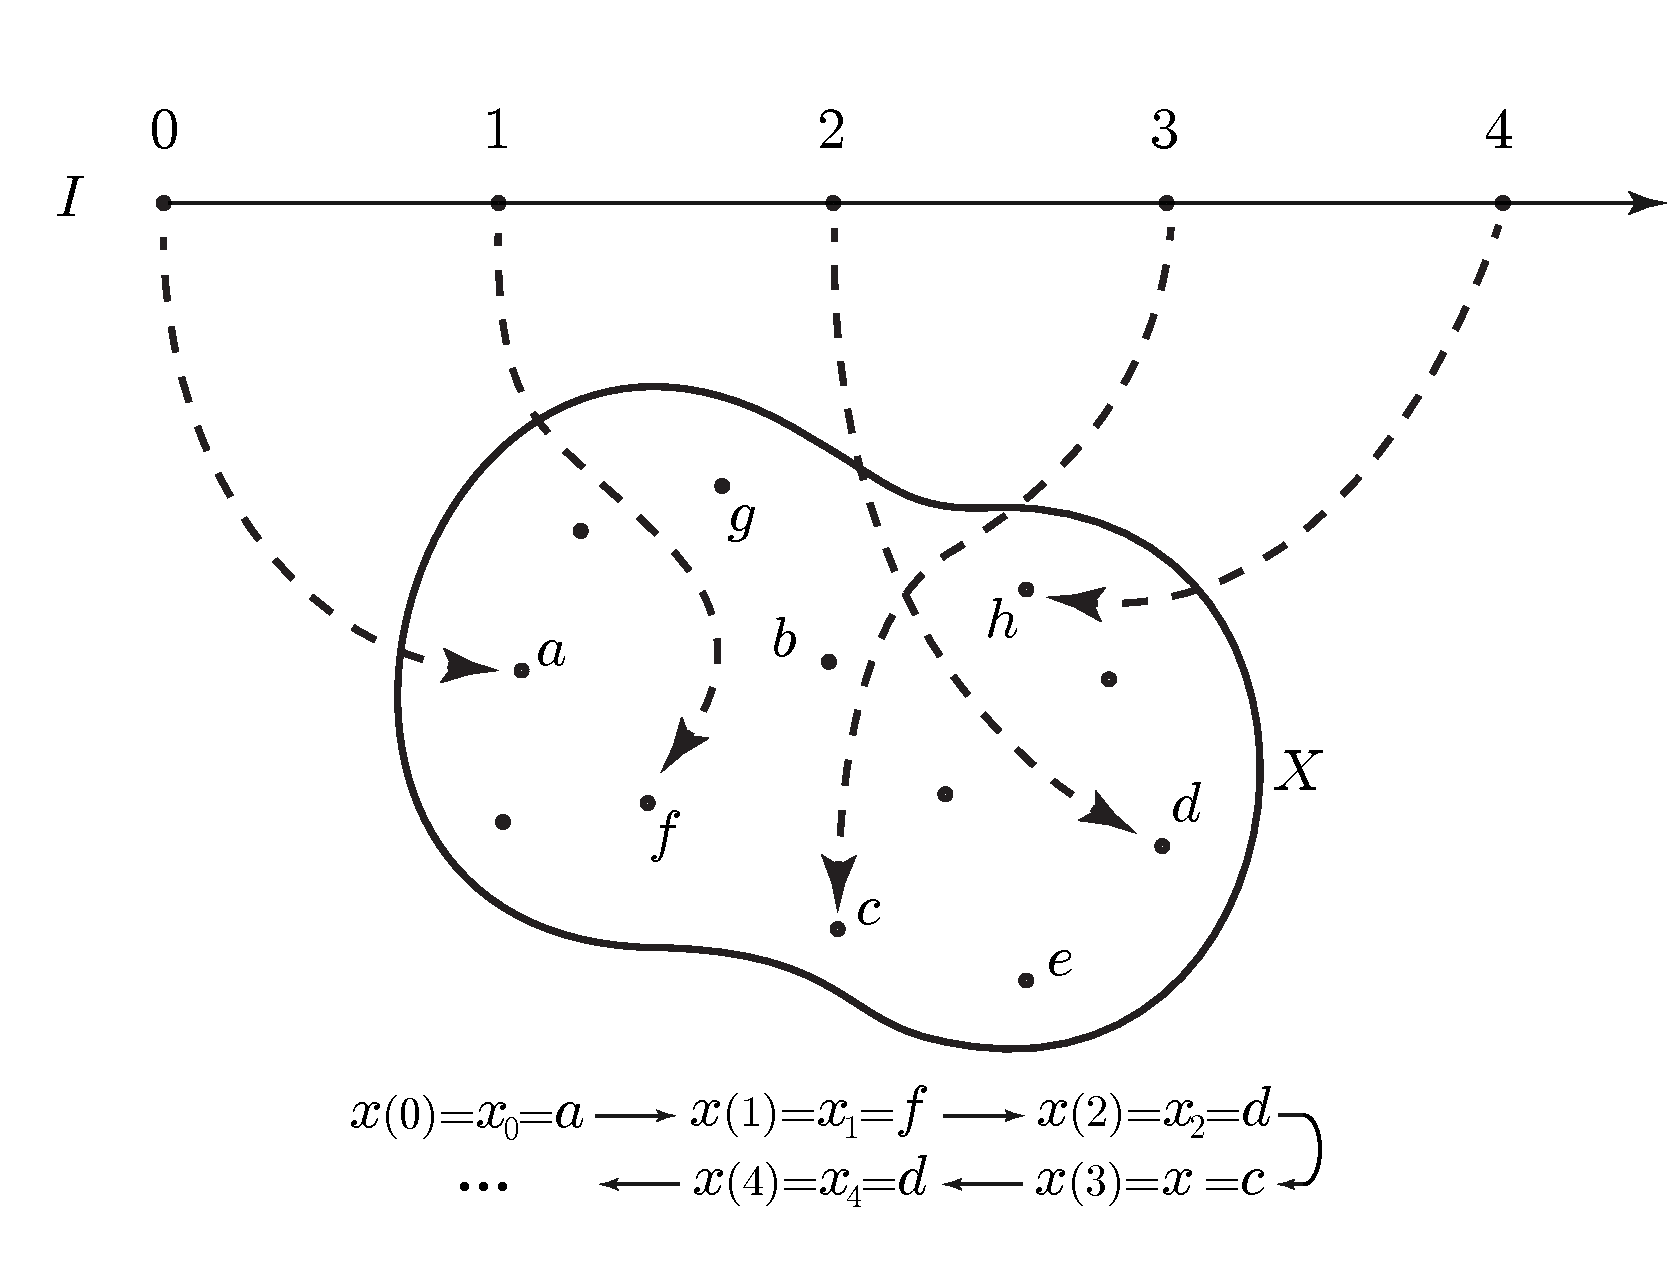
\includegraphics[trim=0cm 0cm 0cm 0cm, clip, scale=0.45]{images/settheorygrafico1.pdf}
\end{center}
È fondamentale che ci sia un \textbf{ordine} su $I$, dato che si vuole confrontare la \textit{posizione} di due elementi della sequenza: un elemento $x_i$ \textit{precede} un altro $x_j$ nella sequenza se gli indici sono tali per cui $i<j$.\\
Per soddisfare la seconda richiesta, ossia che la posizione di un certo elemento nella lista è determinata dalle posizioni degli elementi precedenti, si può pensare di definire la sequenza in modo \textit{ricorsivo}.
Tuttavia, per far ciò, \textit{non} è sufficiente che gli indici siano ordinati. Nello specifico, se $I$ contiene una \textit{sequenza infinita strettamente decrescente}, non siamo sicuri di poter definire ricorsivamente una successione a valori in $X$ indicizzata da $I$.\\
Invece, si può vedere che se $I$ \textit{non} ammette le sequenze infinite strettamente decrescenti, allora le definizioni ricorsive su $I$ sono lecite e permettono di definire univocamente una successione per ogni sequenza di indici! Dobbiamo quindi limitare quali relazioni d'ordine possiamo usare.
\begin{define}[Minimo]
	Se $\left(P,\leq\right)$ è un insieme parzialmente ordinato, $X\neq\emptyset$ un sottoinsieme di $P$ e $a\in X$, allora $a$ è \textbf{minimo}\index{minimo} di $X$ se $a\in X$ e $\forall x\in X,\ a\leq x$. Si indica $a=\min X$.
\end{define}
\begin{define}[Buon ordine]
	Un ordine parziale totale $\leq$ di $P$ è un \textbf{buon ordine} se ogni sottoinsieme $X\neq \emptyset$ di $P$ ha un minimo.
\end{define}
\begin{examples}~{}
	\begin{itemize}
		\item $\left(\naturalset,\leq\right)$ è ben ordinato.
		\item $\integerset,\ \rationalset,\ \realset$ \textit{non} sono ben ordinati rispetto all'ordine canonico $\leq$: tutti ammettono il sottoinsieme $\integerset_{<0}$ degli interi negativi, che non ha minimo.
	\end{itemize}
\end{examples}
\begin{observe}
	Ogni insieme ben ordinato \textit{non} ammette sequenze infinite strettamente decrescenti, in quanto gli elementi della sequenza formano un sottoinsieme e pertanto esso ammette minimo.
\end{observe}
\begin{intuit}
	Possiamo ora capire perché non ha particolarmente senso definire successioni indicizzate, ad esempio, rispetto a $\left(\integerset,<\right)$ o rispetto a $\left(\realset,<\right)$: non ammettendo minimo, non possiamo avere il \textit{passo base} della nostra successione definita ricorsivamente!
\end{intuit}
\begin{digression}
	Il \textbf{teorema del buon ordine}, o anche noto come \textbf{teorema di Zermelo}, afferma che \textit{ogni} insieme non vuoto può essere ben ordinato (rispetto ad un opportuno ordine).\\
	Questo teorema risulta essere vero se si considera valido l'Assioma della Scelta; in realtà, si può ulteriormente mostrare come il teorema del buon ordine risulta essere equivalente, sotto gli Assiomi di Zermelo–Fraenkel, proprio all'Assioma della Scelta!
\end{digression}
Diamo un'ultima definizione, che sarà fondamentale per collegare gli insiemi ben ordinati con gli ordinali.
\begin{define}[Funzioni monotone e isomorfismi d'ordine]
	Siano $\left(P,\leq_P\right)$ e $\left(Q,\leq_Q\right)$ due insiemi parzialmente ordinati. Una funzione $\funz{f}{P}{Q}$ è \textbf{monotona}\index{funzione!monotona} se
	\begin{equation}
		x\leq_P y\implies f(x)\leq_Q f(y)
	\end{equation}
Se una funzione monotona è biettiva e l'\textit{inversa} è monotona, allora $f$ è una \textbf{isotonia}\index{isotonia} o \textbf{isomorfismo d'ordine}.
\end{define}
\section{Ordinali}
Supponiamo di aver preso un insieme degli indici $I$ e, dopo aver posto un buon ordine su di esso, di aver definito una successione nel modo che abbiamo detto nella sezione precedente. Allora, sulla base della definizione intuitiva data nell'introduzione, gli indici scelti fungono proprio da ordinali.\\
Supponiamo ora di prendere un altro insieme di indici $J$ ben ordinati e determinare una successione sulla base di essi. Per questa nuova successione gli elementi di $J$ fanno da ordinale, ma hanno qualcosa in comune con gli indici $I$? Sono gli stessi ordinali o sono ordinali differenti? Potremmo mostrare che c'è un isomorfismo d'ordine tra $I$ e $J$: in questo modo avremmo gli stessi ordinali \textit{a meno di isomorfismo}.\\
Si mostra facilmente che, come ci si aspetterebbe da una funzione chiamata ‘‘isomorfismo'', essere isotonici è una \textbf{relazione di equivalenza} e gli insiemi parzialmente ordinati sono partizionati da essi. Da qui in poi queste classi di equivalenza le chiameremo \textbf{tipi d'ordine}\index{tipo d'ordine}.\\
Georg \textbf{Cantor} (1845 - 1918) definì un numero ordinale proprio come il tipo d'ordine di insiemi \textit{ben ordinati}. Tuttavia, l'indiscutibile appeal intuitivo che questa definizione emana ha due svantaggi:
\begin{enumerate}
	\item I tipi di ordine sono particolarmente ampi: il solo tipo associato all'ordinale $1$, di cui vedremo tra poco la definizione precisa in senso insiemistico, contiene \textbf{tutti} i singoletti, tra cui anche il singoletto $\{1\}$.
	\item In tutte le dimostrazioni che si basano sulle classi di equivalenza è necessario scegliere un rappresentante e controllare che i risultati non dipendono dalla scelta fatta.
\end{enumerate}
Fu John \textbf{von Neumann} (1903-1957)  a proporre un approccio che risolva questi problemi, ma che risulti in tutto e per tutto equivalente alla costruzione originale di Cantor: invece di vedere gli ordinali come classi di equivalenza, definire degli \textit{insiemi canonici} ben ordinati, che chiameremo \textit{ordinali}, e mostrare che ogni insieme ben ordinato è isomorfo ad uno e un solo insieme ordinale. Uno degli aspetti geniali di questa definizione è di definire gli ordinali sulla base degli ordinali che lo precedono, generalizzando ciò che succede per i numeri naturali quando usati per ordinare: un elemento è il \textit{quarto} perché segue il \textit{terzo}, che a sua volta segue il \textit{secondo}, che a sua volta segue il \textit{primo}.\\
Innanzitutto, diamo una definizione formale dei naturali come una famiglia di particolari insiemi costruiti \textit{ricorsivamente dall'insieme vuoto}.
\begin{define}[Numeri naturali]
	I \textbf{numeri naturali} $0,1,2,\ldots$ sono costruiti ricorsivamente nel seguente modo:
	\begin{equation}
		\begin{array}{l}
			0\coloneqq \emptyset\\
			n+1\coloneqq n\cup \left\{n\right\} = \left\{0,\ldots,n\right\}
		\end{array}
	\end{equation}
\end{define}
In altre parole:
\begin{equation*}
	\begin{array}{l}
		0=\left\{\emptyset\right\}\\
		1=\left\{0\right\}=\left\{\emptyset,\left\{\emptyset\right\}\right\}\\
		2=\left\{0,1\right\}=\left\{\emptyset,\left\{\emptyset\right\}, \left\{\emptyset,\left\{\emptyset\right\}\right\}\right\}\\
		\dots
	\end{array}
\end{equation*}
I naturali sono tutti degli insiemi \textit{ben ordinati} e, in particolare, sono anche \textit{transitivi}.
\begin{define}[Transitività]
	Un insieme $T$ è \textbf{transitivo}\index{transitività} se ogni elemento di $T$ è un sottoinsieme di $T$; in altre parole,
	\begin{equation}
		T\subseteq \setpart{T}
	\end{equation}
	o, equivalentemente, se $x\in T$ e $y\in x$, allora $y\in T$.
\end{define}
Possiamo generalizzare la costruzione astratta dei naturali per definire più genericamente i \textit{numeri ordinali}.
\begin{define}[Ordinale]
	Un insieme è un \textbf{ordinale}\index{ordinale} se è transitivo e ben ordinato dalla relazione d'appartenenza $\in$.\\
	Definiamo inoltre una relazione sulla classe di tutti gli ordinali $\mathrm{Ord}$:
	\begin{equation}
		\alpha<\beta\iff\alpha\in\beta
	\end{equation}
\end{define}
\begin{example}
	Per la definizione astratta di naturale, i \textbf{numeri naturali} sono tutti ordinali per definizione.
\end{example}
Dalla sola definizione seguono quasi immediatamente le seguenti proprietà.
\begin{lemmingqed}[Relazioni tra ordinali]
	Valgono le seguenti:
\begin{enumerate}
	\item Se $\alpha$ è un ordinale e $\beta\in\alpha$, allora $\beta$ è un ordinale.
	\item Se $\alpha\neq\beta$ sono ordinali e $\alpha\subsetneqq\beta$, allora $\alpha\in\beta$.
	\item Se $\alpha,\ \beta$ sono ordinali, allora si ha o $\alpha\subseteq\beta$ oppure $\beta\subseteq\alpha$.\qedhere
\end{enumerate}
\end{lemmingqed}
Da questo lemma possiamo ricavare una serie di proprietà importanti:
\begin{itemize}
	\item $<$ è una relazione d'ordine totale nella classe $\mathrm{Ord}$:
	\item Per ogni ordinale $\alpha$ si ha
	\begin{equation*}
		\alpha=\left\{\beta\in\mathrm{Ord} \ \middle| \ \beta<\alpha\right\}
	\end{equation*}
ossia un ordinale contiene \textbf{tutti} gli ordinali che lo precedono.
\item Se $C$ è una classe non vuota di ordinali, allora
\begin{equation*}
	\bigcap C=\inf C\in C
\end{equation*}
è un ordinale
\item Se $X$ è una insieme non vuoto di ordinali, allora
\begin{equation*}
	\bigcup X=\sup X
\end{equation*}
è un ordinale.
\item Per ogni $\alpha$ ordinale, $\alpha\cup\left\{\alpha\right\}$ è un ordinale ed è l'estremo inferiore di tutti gli ordinali che lo seguono.
\begin{equation*}
		\alpha\cup\{\alpha\}=\inf\{\beta\in\mathrm{Ord}\mid\beta>\alpha\}
\end{equation*}
\end{itemize}
\begin{intuit}
	La relazione $<$ indotta da $\in$ sugli ordinali si può vedere come una generalizzazione della relazione d'ordine che conosciamo bene sui naturali. Dopotutto, per essi le due relazioni coincidono!
\end{intuit}
\subsection{Ordinali successori e ordinali limiti}
Data la relazione d'ordine che caratterizzano gli ordinali e sulla base di questi fatti, ha senso definire
\begin{equation*}
	\alpha+1=\alpha\cup\{\alpha\}
\end{equation*}
il \textbf{successore}\index{successore} di $\alpha$.\\
Consideriamo ora un ordinale $\alpha$. Se esiste un ordinale $\beta$ tale per cui $\alpha=\beta+1$, si può dire che $\alpha$ è un \textbf{ordinale successore}. Non è sempre detto che però tale $\beta$ esisti! Un ordinale di questo tipo, per quanto osservato, deve essere successivo a degli ordinali, ma non deve essere il diretto successore di alcun altro ordinale. Utilizzando la terminologia dell'analisi, questo tipo di ordinale è detto \textbf{ordinale limite}\index{ordinale!limite} e
\begin{equation}
	\alpha=\sup\{\beta\in\mathrm{Ord}\mid\beta<\alpha\}=\bigcup\alpha.
\end{equation}
Si considera anche lo \textit{zero} un ordinale limite: si pone $0=\sup\emptyset$.\\
Consideriamo dunque i numeri naturali: ogni numero ha per definizione un successivo e ogni numero è successore di un altro. Segue dunque una domanda esistenziale: c'è qualcosa dopo \textit{tutti} i naturali? La risposta, in teoria degli insiemi, è sì: dopo $0$, $1$, $2$, eccetera, eccetera, si raggiunge un nuovo ordinale, che non è successore di alcun naturale ma che è successivo a tutti: $\omega$.
\begin{define}[Ordinali finiti e transfiniti]
	Si denomina con $\omega$ il più piccolo ordinale limite non zero: esso è il tipo di ordine dei naturali $\naturalset$ e si può identificare con esso.\\
	Gli ordinali prima di $\omega$, ossia i numeri naturali, sono detti ordinali \textbf{finiti}\index{ordinale!finito}, mentre $\omega$ e gli ordinali che seguono sono detti ordinali \textbf{transfiniti}\index{ordinale!transfinito} o \textit{infiniti}.
\end{define}
\begin{intuit}\label{visualizzazioneordinali}
	Come possiamo immaginare gli ordinali transfiniti successivi a $\omega$?\\
	Proviamo prima a guardare agli ordinali da nuovi punti di vista: invece che vederli ‘‘semplicemente'' come insiemi, li possiamo vedere visivamente come sequenze rispetto a $<$, in due modi: la prima è più corretta e fedele alla definizione, mentre la seconda è impropria e - secondo la definizione - errata, ma ci permette di fare alcune intuizioni utili.
	\begin{itemize}
		\item La sequenza di tutti gli ordinali che lo precedono:
		\begin{equation*}
			5\colon 0<1<2<3<4
		\end{equation*}
		\item La sequenza di tutti gli ordinali che lo precedono e l'ordinale stesso:
		\begin{equation*}
			5\colon 0<1<2<3<4\textcolor{red}{<5}
		\end{equation*}
	\end{itemize}
Se $\omega$ è identificato con $\naturalset$, allora le due visualizzazioni sono
	\begin{align*}
		\omega&\colon0<1<2<3<\ldots\\
		\omega&\colon0<1<2<3<\ldots\textcolor{red}{<\omega}
	\end{align*}
La prima visualizzazione coincide la classica rappresentazione dei naturali naturali, mentre la seconda suggerisce qualcos'altro: dopo tutti i naturali ho un elemento nuovo che tuttavia si comporta in modo estremamente simile allo \textit{zero} - dopotutto, non è successore di alcun altro numero, ma ammette un successore.\\
L'idea è quindi di \textbf{rietichettare} $\omega$ con $0'$, $\omega+1$ con $1'$ e così via. In questo modo, un ordinale come $\omega+3$ diventa 
\begin{align*}
	\omega+3&\colon0<1<2<3<\ldots<0'+1'+2'\\
	\omega+3&\colon0<1<2<3<\ldots<0'+1'+2'\textcolor{red}{+3'}
\end{align*}
Questo ragionamento permette di immaginare numeri più complessi: l'ordinale $\omega+\omega$ coincide con due copie dei naturali, la cui seconda copia segue completamente alla destra della prima:
\begin{align*}
	\omega+\omega&\colon0<1<2<3<\ldots<0'<1'<2'<3'<\ldots\\
	\omega+\omega&\colon0<1<2<3<\ldots<0'<1'<2'<3'<\ldots\textcolor{red}{<0''}
\end{align*}
\end{intuit}
Gli ordinali $\omega,\ \omega+1,\ \ldots, \omega\cdot 2,\ \ldots \omega^{\omega}\cdot $ sono tutti ordinali numerabili e riguardando l'ordinamento di insiemi infiniti detti \textit{numerabili}. L'ordinale limite che segue dopo tutti gli ordinali numerabili è indicato come $\omega_1$ ed è il primo ordinale non numerabile.\\ 
Concludiamo la sezione con una definizione che successivamente riprenderemo quando parleremo di cardinalità.
\begin{define}[Insiemi finiti e infiniti.]
	Un insieme $X$ è detto \textbf{finito}\index{insieme!finito} se c'è una biezione tra $X$ e un naturale $n\in\naturalset$, con $n$ inteso come insieme.\\
	Se $X$ non è finito è detto \textbf{infinito}\index{insieme!infinito}.
\end{define}
\subsection{Isomorfismo dell'ordinale con gli insiemi ben ordinati}
Concludiamo senza dare dimostrazione il teorema che permette di concludere la definizione di ordinale secondo von Neumann.
\begin{theoremaqed}[Isotonia tra ordinali e insiemi ben ordinati]
	Ogni insieme ben ordinato è isomorfo ad un unico ordinale.
\end{theoremaqed}
Questo è il motivo per cui si può identificare $\omega$ con $\naturalset$: l'insieme dei naturali è un insieme ben ordinato e si può mostrare l'isomorfismo d'ordine con il più piccolo ordinale limite non nullo.
\subsection{Induzione transfinita}
Ricordiamo uno dei modi per enunciare l'\textit{induzione} sui naturali. 
\begin{theoremaqed}[Induzione]
	Sia $A$ un sottoinsieme di $\naturalset$ e si supponga che
	\begin{enumerate}
		\item $0\in A$.
		\item Se $n\in A$, allora $n+1\in A$.
	\end{enumerate}
	Allora $A=\naturalset$.
\end{theoremaqed}
Con ciò che abbiamo introdotto possiamo generalizzare facilmente questa proprietà agli ordinali anche non finiti.
\begin{theorema}[Induzione transfinita]
	Sia $C$ una classe di ordinali e si supponga che
	\begin{enumerate}
		\item $0\in C$.
		\item Se $\alpha\in C$, allora $\alpha+1\in C$.
		\item Se $\alpha$ è un ordinale limite non zero e si ha $\beta\in C,\ \forall \beta<\alpha$, allora $\alpha\in C$.
	\end{enumerate}
Allora $C=\mathrm{Ord}$.
\end{theorema}
\begin{demonstration}
	Se $C=\mathrm{Ord}$ abbiamo finito. Altrimenti, sia $\alpha$ il più piccolo ordinale\footnote{Possiamo farlo in quanto un ordinale è ben ordinato} che \textit{non} appartiene a $C$.
	\begin{itemize}
		\item Se $\alpha=0$ si ha subito l'assurdo per l'ipotesi $1$.
		\item Se $\alpha$ è un ordinale successore, allora sia $\beta$ l'ordinale tale per cui $\alpha=\beta+1$: per contronominale sulla ipotesi 2. si ha
		\begin{equation*}
			\alpha=\beta+1\notin C\implies \beta\notin C,
		\end{equation*}
		ma allora essendo $\beta<\alpha$ si ha una contraddizione perché $\alpha$ non è più il più piccolo ordinale non in $C$.
		\item Se $\alpha$ è un ordinale limite non nullo, allora per contronominale sull'ipotesi $3.$ si ha che
		\begin{equation*}
			\exists \beta<\alpha\colon\beta\notin C
		\end{equation*}
		e come prima essendo $\beta<\alpha$ si ha una contraddizione perché $\alpha$ non è più il più piccolo ordinale non in $C$.\qedhere
	\end{itemize}
\end{demonstration}
\subsection{Sequenze e limite}
Diamo ora una definizione di \textit{successione}, che abbiamo finora visto solo intuitivamente.
\begin{define}[Successione]
	Una successione è una funzione il cui dominio è un ordinale $\alpha$. La notazione canonica per una sequenza è
	\begin{equation*}
		\left<a_\xi \ \middle| \ \xi<\alpha\right>
	\end{equation*}
\end{define}
\begin{examples}~
	\begin{itemize}
		\item Una successione finita è una funzione sul dominio finito $\left\{i\in\naturalset\mid i<n\right\}$ per qualche $n\in\naturalset$. Viene anche detta anche \textbf{sequenza di lunghezza} $n$.
		\item Una successione nel senso classico del termine è una funzione su $\naturalset$ o, equivalentemente, sull'ordinale $\omega$. Si può indicare come
			\begin{equation*}
			\left<a_n \ \middle| \ n<\omega\right>
		\end{equation*}
	\end{itemize}
\end{examples}
\begin{define}[Limite di una successione]
	Sia $\alpha>0$ un ordinale limite e sia $\left<\gamma_\xi \ \middle| \ \xi<\alpha\right>$ una successione \textbf{non decrescente} di ordinali, cioè
	\begin{equation*}
		\xi <\eta \implies \gamma_\xi\leq \gamma_\eta.
	\end{equation*}
	Si definisce il \textbf{limite}\index{limite} di una successione
	\begin{equation}
		\lim_{\eta\to \alpha}\gamma_\xi=\sup\left\{\gamma_\xi\mid\xi<\alpha\right\}
	\end{equation}
\end{define}
\subsection{Aritmetica degli ordinali}
\paragraph{Addizione}
\begin{define}[Addizione di ordinali]
	Per ogni ordinale $\alpha$ si ha
	\begin{enumerate}
		\item \textbf{Zero come identità:}
		$\alpha+0=\alpha$
		\item \textbf{Associatività:}
		\begin{equation*}
			\alpha+\left(\beta+1\right)=\left(\alpha+\beta+1\right),\ \forall \beta
		\end{equation*}
		Più in generale, si ha
		\begin{equation*}
			\alpha+\left(\beta+\gamma\right)=\left(\alpha+\beta\right)+\gamma,\ \forall \beta,\ \forall\gamma
		\end{equation*}
		\item \textbf{Somma come limite:}
		\begin{equation*}
			\alpha+\beta=\lim_{\eta\to\beta}\left(\alpha+\eta\right),\ \text{per ogni ordinale limite}\ \beta>0
		\end{equation*}
	\end{enumerate}
\end{define}
\begin{attention}
	L'addizione di ordinali \textbf{non} è commutativa. Ad esempio, $1+\omega=\omega\neq\omega+1$.
\end{attention}
\begin{intuit}
	Prima di dimostrarlo formalmente, cerchiamo di capire intuitivamente perché questo non accade. Riprendendo la prima delle due visualizzazioni introdotta a pag. \pageref{visualizzazioneordinali}, scriviamo $1+\omega$ e $\omega+1$, dove etichettiamo $\omega$ con $0'$.
	\begin{align*}
		1+\omega&\colon0<0'<1'<2'<3'<\ldots\\
		\omega+1&\colon0<1<2<3<\ldots<0'
	\end{align*}
	Notiamo che nel primo caso $0'$ (cioè $\omega$) ha un predecessore, $0$, cosa che normalmente \textit{non} ha; rinominando $n'$ con $n+1$ otteniamo che la sequenza assomiglia in realtà a $\omega$ stesso, cioè possiamo dire che $1+\omega=\omega$. D'altro canto, $\omega+1$ ha un elemento massimo, che è $0'$, mentre $\omega$ non lo ha!
\end{intuit}
\begin{examplewt}[Non commutatività dell'addizione di ordinali]
	Mostriamo che
	\begin{equation*}
		1+\omega=\omega\neq\omega+1
	\end{equation*}
 	Infatti, il termine di sinistra diventa
 	\begin{align*}
 		1+\omega&=\lim_{\eta\to \omega}\left(1+\xi\right)=\sup\left\{1+\xi \ \middle| \ \xi<\omega\right\}=\bigcup_{\xi<\omega}\left\{1+\xi\right\}=\\
 		&=1\cup 2\cup 3\cup \ldots=\{0\}\cup\{0,1\}\cup\{0,1,2\}\cup\ldots\naturalset=\omega
 	\end{align*}
 	e per definizione $\omega<\omega+1$ e dunque sono due ordinali distinti.
\end{examplewt}
In realtà è molto raro che $\alpha+\beta$ sia uguale a $\beta+\alpha$: ciò succede se e solo se $\alpha=\gamma \cdot m$ e $\beta=\gamma \cdot n$ con $\gamma$ ordinale e $m,\ n$ naturali e $\cdot$ la moltiplicazione tra ordinali che vedremo tra poco.
\paragraph{Moltiplicazione}
\begin{define}[Moltiplicazione di ordinali]
	Per ogni ordinale $\alpha$ si ha
	\begin{enumerate}
		\item \textbf{Zero come elemento nullo:}
		$\alpha\cdot0=0$
		\item \textbf{Distributiva da sinistra:}
		\begin{equation*}
			\alpha\cdot\left(\beta+1\right)=\alpha\cdot\beta+\alpha,\ \forall \beta
		\end{equation*}
		\item \textbf{Associativa:}
		\begin{equation*}
			\alpha\cdot\left(\beta\cdot\gamma\right)=\left(\alpha\cdot\beta\right)\cdot\gamma,\ \forall \beta,\ \gamma
		\end{equation*}
		\item \textbf{Prodotto come limite:}
		\begin{equation*}
			\alpha\cdot\beta=\lim_{\eta\to\beta}\left(\alpha\cdot\eta\right),\ \text{per ogni ordinale limite}\ \beta>0
		\end{equation*}
	\end{enumerate}
\end{define}
\begin{attention}
	La moltiplicazione di ordinali \textbf{non} è commutativa e neanche distributiva da destra. Ad esempio, $\left(1+1\right)\cdot\omega=\omega\neq\omega\cdot\left(1+1\right)=\omega+\omega$.
\end{attention}
\begin{examplewt}[Non commutatività della moltiplicazione di ordinali]
	Mostriamo che
	\begin{equation*}
		\left(1+1\right)\cdot\omega=2\omega=\omega\neq\omega\cdot\left(1+1\right)=\omega\cdot 2=\omega+\omega
	\end{equation*}
	Infatti, il termine di sinistra diventa
	\begin{align*}
		\left(1+1\right)\cdot\omega&=2\cdot\omega=\lim_{\eta\to \omega}\left(2\cdot\xi\right)=\sup\left\{2\cdot\xi \ \middle| \ \xi<\omega\right\}=\bigcup_{\xi<\omega}\left\{2\cdot\xi\right\}=\\
		&=2\cdot 0\cup2\cdot 1\cup 2\cdot2\cup 2\cdot3\cup \ldots=0\cup 2\cup 6\cup\ldots=\\
		&=\emptyset\cup\{0,1\}\cup\{0,1,2,3,4,5\}\cup\ldots=\naturalset=\omega
	\end{align*}
	e per definizione $\omega<\omega+\omega$ e dunque sono due ordinali distinti.
\end{examplewt}
\paragraph{Esponenziazione}
\begin{define}[Esponenziazione di ordinali]
		Per ogni ordinale $\alpha$ si ha
	\begin{enumerate}
		\item \textbf{Esponenziazione per zero:}
		$\alpha^0=1$
		\item \textbf{Distributiva dell'esponenziale rispetto all'esponente:}
		\begin{equation*}
			\alpha^{\beta+1}=\alpha^\beta\cdot\alpha,\ \forall \beta
		\end{equation*}
		\item \textbf{Prodotto come limite:}
		\begin{equation*}
			\alpha^{\beta}=\lim_{\eta\to\beta}\left(\alpha^\eta\right),\ \text{per ogni ordinale limite}\ \beta>0
		\end{equation*}
	\end{enumerate}
\end{define}
\paragraph{Aritmetica degli ordinali e aritmetica degli interi}
Abbiamo visto che le operazioni con i numeri ordinali hanno notevoli differenze da queste 
\begin{property}[Aritmetica degli ordinali e aritmetica degli interi]
	Valgono le seguenti proprietà:
	\begin{enumerate}
		\item Se $\beta<\gamma$, allora
		\begin{equation*}
			\alpha+\beta<\alpha+\gamma,\ \forall \alpha.
		\end{equation*}
		\item Se $\alpha<\beta$, allora esiste un unico $\delta$ tale che \begin{equation*}
			\alpha+\delta=\beta.
		\end{equation*}
		\item Se $\beta<\gamma$, allora
		\begin{equation*}
			\alpha\cdot \beta<\alpha\cdot\gamma,\ \forall \alpha>0.
		\end{equation*}
		\item Se $\alpha>0$ e $\gamma$ è un ordinale arbitrario, allora esiste un unico $\beta$ e un unico $\rho<\alpha$ tale che
		\begin{equation*}
			\gamma=\alpha\cdot\beta+\rho.
		\end{equation*}
		\item Se $\beta<\gamma$ e $\alpha>1$, allora
		\begin{equation*}
			\alpha^{\beta}<\alpha^{\gamma}.\qedhere
		\end{equation*}
	\end{enumerate}
\end{property}
\begin{theoremaqed}[Teorema della forma normale di Cantor]
	Ogni ordinale $\alpha>0$ può essere rappresentato unicamente nella forma
	\begin{equation}
		\alpha=\sum_{i=1}^{+\infty}\omega^{\beta_i}\cdot k_i=\omega^{\beta_1}\cdot k_1+\cdot+\omega^{\beta_n}\cdot k_n
	\end{equation}
dove $n\geq 1,\ \alpha\geq \beta_1>\ldots>\beta_n$ e $k_1,\ \ldots, k_n$ sono naturali non nulli.
\end{theoremaqed}
Dal teorema della forma normale è possibile che ci siano degli ordinali $\alpha$ tali che
\begin{equation*}
	\alpha=\omega^{\alpha}
\end{equation*}
Il più piccolo di questi ordinali è indicato con $\epsilon_0$.
\section{Cardinalità}
\begin{comment}

\end{comment}
\begin{define}[Cardinalità]
	Due insiemi $X$ e $Y$ sono \textbf{equipotenti}\index{equipotenza} o \textbf{equinumerosi}\index{equinumerosità}, in simboli
	\begin{equation}
		X\asymp Y
	\end{equation}
	se esiste una corrispondenza \textit{biunivoca} tra i due insiemi.\\
	L'equipotenza è una \textit{relazione di equivalenza} sulle classi di tutti gli insiemi; diciamo che due insiemi $X$ e $Y$ equipotenti hanno la stessa \textbf{cardinalità}\index{cardinalità} e lo indichiamo con
	\begin{equation}
		\abs{X}=\abs{Y}
	\end{equation}
\end{define}

\subsection{Ordine delle cardinalità}
\begin{define}[Iniezione]
	Un insieme $X$ si \textbf{inietta in} $Y$, in simboli 
	\begin{equation}
		X\precsim Y
	\end{equation}
	se esiste una funzione iniettiva $\funz{f}{X}{Y}$; in tal caso scriveremo
	\begin{equation}
		\abs{X}\leq\abs{Y}
	\end{equation}
\end{define}
\begin{corollary}[Inclusione e cardinalità]\label{cardinalitàinclusione}
	Se $X\subseteq Y$, allora $X\precsim Y$ (o in termini di cardinalità, $\abs{X}\leq\abs{Y}$).
\end{corollary}
\begin{demonstration}
	Dire che $X\subseteq Y$ implica l'esistenza dell'inclusione $\incl{\iota}{X}{Y}$, la quale è per definizione una funzione iniettiva.
\end{demonstration}
\begin{attention}\label{cardinalitàugualenonimplicauguaglianzainsiemistica}
	Anche se un sottoinsieme ha la stessa cardinalità dell'insieme a cui appartiene, non è detto che siano uguali; come controesempio basta considerare i numeri naturali $\naturalset$ e numeri pari $2\naturalset$: fra i due c'è una biezione $\funz{\ }{\naturalset}{2\naturalset}$ data da $f(n)=2n$, ma i naturali contengono anche i dispari.\\
	Si può invece affermare che un sottoinsieme \textbf{finito} equipotente all'insieme a cui appartiene deve coincidere con esso.
\end{attention}
La relazione $\precsim$ (o $\leq$ se ci riferiamo alle cardinalità) è una relazione d'\textit{ordine totale}: la relazione riflessiva e transitiva sono immediate, mentre l'antisimmetrica è garantita dal seguente teorema.
\begin{theoremaqed}[Teorema di Cantor-Bernstein-Schröder]
	Se $\abs{X}\leq\abs{Y}$ e $\abs{Y}\leq\abs{X}$, allora $\abs{X}=\abs{Y}$.\\
	Equivalentemente, se esistono due funzioni \textit{iniettive}
	\begin{equation*}
		\funz{f}{X}{Y}\text{ e }\funz{g}{Y}{X}
	\end{equation*}
	allora esiste una funzione \textit{biettiva} $\funz{h}{X}{Y}$.
\end{theoremaqed}
Un'altra conseguenza importante di questo teorema è quella di poter determinare la cardinalità sulla base di sole funzioni \textit{iniettive}.
\begin{examplewt}[Un'applicazione del teorema di Cantor-Bernstein-Schröder]
	L'intervallo $\left[0,1\right]$ ha la cardinalità del continuo; infatti, possiamo considerare le seguenti funzioni iniettive:
	\begin{itemize}
		\item $\incl{\iota}{\left[0,1\right]}{\realset}$ inclusione.
		\item $\funztot{f}{\realset}{\left[0,1\right]}{x}{\frac{2\left(\arctan(x)+\frac{\pi}{2}\right)}{\pi}}$
	\end{itemize}
\end{examplewt}
La seguente proposizione permette invece stabilire una relazione di cardinalità tra dominio e codominio di una funzione \textit{suriettiva}.
\begin{proposition}[La cardinalità del dominio di una funzione suriettiva è maggiore o uguale della cardinalità del codominio]\label{cardinalitàsuriettiva}
	Sia $\surr{g}{Y}{X}$ suriettiva, con $\left(Y,\unlhd\right)$ un insieme ben ordinato. Allora esiste una funzione iniettiva $\funz{f}{X}{Y}$ tale che $g\circ f=id_X$. In altre parole,
	\begin{equation}
		\surr{g}{\left(Y,\unlhd\right)}{X}\implies X\precsim Y \left( \iff \abs{X}\leq\abs{Y}\right).\qedhere
	\end{equation}
\end{proposition}
\begin{demonstration}
	Si definisce $f$ in modo che $f(x)$ è il minimo y$\in Y$, rispetto a $\unlhd$, per cui $g\left(y\right)=x$.
\end{demonstration}
\begin{attention}
	È fondamentale l'ipotesi del buon ordine su $Y$: per insiemi non ben ordinati, la proprietà non si verifica perché non si potrebbe scegliere a priori un elemento da fissare. Tuttavia, se si assume l'Assioma della Scelta come vero allora questa proprietà è verificata per ogni insieme.
\end{attention}
\begin{example}
	Come visto\footnote{Si veda \refChapterOnly{teoriamisura}, pag. \pageref{insiemecantor}.}, dato l'insieme di Cantor $C$ si può definire una funzione $\surr{f}{C}{\left[0,1\right]}$ \textit{suriettiva}; in questo modo, $\abs{C}\geq \left[0,1\right]$ ma, in quanto $C\subseteq \left[0,1\right]$ si ha 
	\begin{equation*}
		\abs{C}=\left|\left[0,1\right]\right|
	\end{equation*}
Questa è anche una conseguenza del teorema di Cantor–Bernstein–Schröder, dato che abbiamo definito (implicitamente o esplicitamente) due funzioni iniettive $\funz{\ }{X}{Y}$ e $\funz{\ }{Y}{X}$.
\end{example}
Ci interessa anche definire una relazione d'\textit{ordine parziale forte} sulla base dell'iniezione precedentemente definita. 
\begin{define}[Iniezione stretta]
	Un insieme $X$ si \textbf{inietta strettamente in} $Y$, in simboli 
	\begin{equation}
		X\precnsim Y
	\end{equation}
	se esiste una funzione iniettiva $\funz{f}{X}{Y}$ ma non esistono funzioni suriettive $\funz{f}{X}{Y}$; in tal caso scriveremo
	\begin{equation}
		\abs{X}<\abs{Y}
	\end{equation}
\end{define}
\begin{observe}
	Si può vedere che
	\begin{equation}
		X \precnsim Y\iff X\precsim Y\wedge X\cancel\asymp Y
	\end{equation}
	o, in termini di cardinalità,
	\begin{equation}
		\abs{X}<\abs{Y}\iff \abs{X}\leq \abs{Y}\wedge \abs{X}\neq\abs{Y}
	\end{equation}
\end{observe}
\subsection{Aritmetica dei cardinali}
Possiamo definire delle \textit{operazioni aritmetiche} con i cardinali; dati $\abs{X}=\kappa$ e $\abs{Y}=\lambda$, si ha
\begin{align}
	\kappa+\lambda&=\abs{X\cup Y} \text{ se }X\text{ e }Y\text{ disgiunti}\\
	\kappa\cdot\lambda&=\abs{X\times Y}\\
	\kappa^{\lambda}&=\abs{X^Y}
\end{align}
dove con $X^Y$ indichiamo l'\textit{insieme delle funzioni} da $Y$ in $X$.\\
Queste operazioni sono ben definite se sono indipendenti dalla scelta di $X$ e $Y$.
\begin{property}[Proprietà dell'aritmetica dei cardinali]
	Valgono le seguenti proprietà:
	\begin{enumerate}
		\item L'addizione $+$ e la moltiplicazione $\cdot$ sono associative, commutative e distributive.
		\item \textbf{Distributività dell'esponenziale rispetto alla base:}
		\begin{equation}
			\left(\kappa\cdot\lambda\right)^{\mu}=\kappa^{\mu}\cdot\lambda^{\mu}
		\end{equation}
		\item \textbf{Distributività dell'esponenziale rispetto all'esponente:}
		\begin{equation}
			\kappa^{\lambda+\mu}=\kappa^{\lambda}\cdot\kappa^{\mu}
		\end{equation}
		\item \textbf{Esponenziale di un esponenziale:}
		\begin{equation}
			\left(\kappa^{\lambda}\right)^{\mu}=\kappa^{\lambda\cdot\mu}
		\end{equation}
		\item Se $\lambda\leq \mu$, allora
		\begin{equation}
			\kappa^{\mu}\leq \lambda^{\mu}
		\end{equation}
	%NOTA: are you sure about that?
		\item Se $0<\lambda\leq \mu$, allora
		\begin{equation}
			\kappa^{\lambda}\leq \kappa^{\mu}
		\end{equation}
		\item Se $\kappa>0$, allora
		\begin{equation}
			\kappa^0=1\qquad 1^{\kappa}=1\qquad 0^\kappa=0
		\end{equation}
	\end{enumerate}
\end{property}
\subsection{Cardinalità dell'insieme delle parti}
Finché operiamo con insiemi finiti, è chiara la differenza tra le dimensioni di due insiemi; la questione è differente se si parla di insiemi infiniti: non sempre è immediata la cardinalità. Ad esempio, i numeri pari e i naturali hanno la stessa cardinalità (basta considerare $f(n)=2n$) come biezione, ma i naturali sembrano molto più grandi.\\
Si potrebbe pensare che tutti gli insiemi infiniti hanno la stessa cardinalità. Il seguente teorema ci mostra come questo \textit{non} sia il caso, e la cardinalità è un aspetto fondamentale dello studio degli insiemi infiniti.
\begin{theorema}[Teorema di Cantor]
	Per ogni insieme $X$ si ha
	\begin{equation}
		X\precnsim\setpart{X}
	\end{equation}
	\begin{equation}
		\abs{X}<\abs{\setpart{X}}
	\end{equation}
\end{theorema}
\begin{demonstration}
	Sia per assurdo $\funz{f}{X}{\setpart{X}}$ una funzione suriettiva e sia
	\begin{equation*}
		Y=\left\{x\in X\mid x\notin f(x)\right\}
	\end{equation*}
	Per la suriettività di $f$, $\exists z\in X$ tale che $f\left(z\right)=Y$; tuttavia, si ha $z\in Y\iff z\notin f\left(z\right)=Y$, il che è assurdo. Segue che $X\nasymp\setpart{X}$.\\
	Invece, la funzione
	\begin{equation*}
		\funztot{f}{X}{\setpart{X}}{x}{\left\{x\right\}}
	\end{equation*}
	è iniettiva e quindi $X\precsim\setpart{X}$. Concludendo, $X\precnsim\setpart{X}$.
\end{demonstration}
\begin{theoremaqed}[Biezione tra {$\setpart{X}$} e insieme delle funzioni da {$X$} in {$\{0,1\}$}]\label{cardinalitàsetpart}
	Dato un qualunque insieme $X$, sia $\setpart{X}$ l'insieme delle parti di $X$ e sia $2^X\coloneqq\left\{0,1\right\}^X$ l'insieme di tutte le funzioni $\funz{\ }{X}{\left\{0,1\right\}}$. Allora esiste una biezione tra $\setpart{X}$ e $2^X$, data da
	\begin{equation}
		\funztot{\Phi}{\setpart{X}}{2^X}{X}{\chi_X}
	\end{equation}
	con $\chi_X$ la \textit{funzione indicatrice} su $X$; l'inversa di tale funzione è la seguente:
	\begin{equation}
		\funztot{\Phi^{-1}}{2^X}{\setpart{X}}{f}{\left\{x\in\ X\mid f(x)=1\right\}}\qedhere
	\end{equation}
\end{theoremaqed}
\begin{demonstration}
	Per il teorema precedente, si ha una biezione tra $\setpart{X}$ e $2^{\abs{X}}\coloneqq\left\{0,1\right\}^{X}$, dunque hanno la stessa cardinalità. Per esponenziazione dei cardinali, si ha
	\begin{equation*}
		\abs{\setpart{X}}=\left|\left\{0,1\right\}^{X}\right|=\left|\left\{0,1\right\}\right|^{\abs{X}}=2^{\abs{X}}\qedhere
	\end{equation*}
\end{demonstration}
\begin{corollary}[Cardinalità dell'insieme delle parti]\label{insiemiparti}
	Se un insieme $X$ ha cardinalità $\abs{X}$, l'insieme delle parti ha cardinalità
	\begin{equation}
		\abs{\setpart{X}}=2^{\abs{X}}
	\end{equation}
\end{corollary}
Il teorema di Cantor si può quindi riformulare come segue
\begin{theoremaqed}[Teorema di Cantor, riformulato]
	Per ogni cardinale $\kappa$ si ha $\kappa<2^{\kappa}$.
\end{theoremaqed}
\subsection{Ordinali e cardinali}
Sappiamo che gli ordinali, per definizione di von Neumann, sono degli insiemi. Possiamo dare una definizione di \textit{numero cardinale} partendo proprio dal concetto di ordinale.
\begin{define}[Cardinale]
	Un ordinale $\alpha$ è detto un \textbf{cardinale}\index{cardinale} se
	\begin{equation}
		\abs{\alpha}\neq\abs{\beta},\ \forall \beta<\alpha
	\end{equation}
\end{define}
Se $W$ è un insieme ben ordinato, sappiamo che esso ha un tipo d'ordine e dunque almeno un ordinale ad esso associato. Allora consideriamo, dato $W$, il suo numero cardinale come
\begin{equation*}
	\abs{W}=\min\{\alpha\in\mathrm{Ord}\mid\abs{W}=\abs{\alpha}\}
\end{equation*}
Ricordiamo che $X$ è \textit{finito} se è in corrispondenza biunivoca con un \textit{ordinale finito} $n\in\naturalset$:
\begin{equation*}
	\abs{X}=\abs{n}
\end{equation*}
Poichè $\abs{n}=\abs{m}\iff n=m$, gli \textit{ordinali finiti} corrispondono ai \textit{cardinali finiti} e quindi $\abs{n}=n$, ossia
\begin{equation*}
	\abs{X}=n
\end{equation*}
L'ordinale $\omega$ è il più piccolo numero cardinale infinito. 
\begin{observe}
	Tutti i cardinali infiniti sono ordinali limiti.
\end{observe}
Gli ordinali infiniti che sono anche cardinali sono chiamati \textbf{aleph}\index{aleph}.
\begin{lemming}[Successori dei cardinali]
	Si può mostrare che per ogni cardinale $\alpha$ c'è un cardinale più grande di esso. Il più piccolo tra quelli più grandi di $\alpha$ viene indicato con $\alpha^{+}$ ed è detto il \textbf{cardinale successore}\index{cardinale!successore}.
\end{lemming}
In particolare, consegue anche che se $X$ è un insieme di cardinali $\sup X$ è un cardinale.\\
Definiamo allora l'enumerazione degli aleph. Indichiamo normalmente $\aleph_{\alpha}$ per i numeri cardinali e $\omega_\alpha$ per il tipo di ordine.
\begin{align*}
	\aleph_0&=\omega_0=\omega\\
	\aleph_{\alpha+1}&=\alpha_{\alpha}^{+}=\omega_{\alpha+1}\\
	\aleph_{\alpha}&=\omega_{\alpha}=\sup\left\{\omega_\beta\mid \beta<\alpha\right\}\quad\text{se}\ \alpha\ \text{è un ordinale limite}
\end{align*}
In questo modo, affermiamo che
\begin{equation}
	\abs{\naturalset}=\aleph_0
\end{equation}
Inoltre, poiché si può mostrare che $\integerset$ e $\rationalset$ sono in biezione con i naturali, anche loro hanno cardinalità $\aleph_0$.
\begin{observe}
	Dalla definizione si nota un fatto fondamentale: ci possono essere più ordinali per uno stesso cardinale. Come mai?\\
	Gli ordinali descrivono in che maniera (a meno di rietichettare i miei elementi) posso ordinare un insieme, mentre i cardinali sono una misura della dimensione di tale insieme.\\ Finché ci limitiamo ai naturali, come ben sappiamo, non c'è differenza tra ordinale e cardinale. Anzi! Ad ogni numero naturale associamo un solo ordinale e un solo cardinale - ad esempio, se devo ordinare l'insieme $\{1,2,3,4\}$ - che ha cardinalità $4$ - non importa se metto prima il 2 dell'1 o il 3 dopo il 4, dato che rinominando gli elementi ottengo sempre l'ordine canonico $0<1<2<3$.\\
	Caso differente è per gli insiemi infiniti. Ad esempio, sui naturali posso avere l'ordinamento canonico $\omega$, ma posso anche riordinarli mettendo prima tutti i naturali dispari seguiti da tutti i naturali pari:
	\begin{equation*}
		1<3<5<7<9<\ldots<2<4<6<8<10<\ldots
	\end{equation*}
	Questo ordinamento quale ha tipo d'ordine $\omega\cdot 2\neq \omega$. Tuttavia, entrambi sono ordinamenti dei naturali e quindi hanno cardinalità $\aleph_0$.
\end{observe}
La somma e il prodotto di aleph è abbastanza triviale, dato che si può mostrare che:
\begin{equation*}
	\aleph_{\alpha}+\aleph_{\beta}=\aleph_{\alpha}\cdot\aleph_{\beta}=\max\{\aleph_{\alpha},\aleph_{\beta}\}
\end{equation*}
\subsection{Cardinalità del continuo}
Abbiamo definito i cardinali per insiemi \textit{ben ordinati}, basandoci sugli ordinali. In realtà, se supponiamo l'\textit{Assioma di Scelta}, allora \textit{ogni insieme} è ben ordinato e quindi possiamo parlare di cardinali in generale in $\mathsf{ZFC}$, anche per insiemi come i \textit{reali}.
\begin{theoremaqed}[Cantor]
L'insieme dei numeri reali non è numerabile, ossia è un insieme infinito che non è in corrispondenza biunivoca con i naturali.
\end{theoremaqed}
Indichiamo con $\mathfrak{c}$ la \textbf{cardinalità dei reali} o \textbf{cardinalità del continuo}\index{cardinalità!del continuo}:
\begin{equation}
	\abs{\realset}=\mathfrak{c}
\end{equation}
Che valore ha questa cardinalità?\\
Poiché siamo in grado di calcolare la cardinalità dell'insieme delle parti di insiemi per il corollario \ref{insiemiparti}, si ha che $\abs{\setpart{\naturalset}}=2^{\aleph_{0}}$.\\
Dato che ogni numero reale è l'estremo superiore di un'opportuna sequenza di razionali minori di essa, cioè
\begin{equation*}
	r=\sup\{q\in\rationalset\mid q<r\},
\end{equation*}
si ha che la cardinalità dei reali deve essere minore dell'insieme delle sequenze in $\rationalset$, che ha cardinalità pari all'insieme delle parti di $\rationalset$, ovvero
\begin{equation*}
	\mathfrak{c}\leq\abs{\setpart{\rationalset}}=2^{\aleph_0}
\end{equation*}
D'altro canto, l'insieme di Cantor\footnote{Si veda \refChapterOnly{teoriamisura}, pag. \pageref{insiemecantor}.} si vede che è in corrispondenza diretta con tutte le sequenze di $0$ e $2$ e la cardinalità coincide con quella di $2^{\aleph_0}$. Poiché Cantor è un sottoinsieme dei reali, si ha
\begin{equation*}
	\mathfrak{c}\geq \abs{C}=2^{\aleph_0}
\end{equation*}
e quindi si può concludere per Cantor-Bernstein-Schröder che
\begin{equation*}
	\mathfrak{c}=2^{\aleph_0}
\end{equation*}
Una peculiarità di questo cardinale è che nella teoria $\mathsf{ZFC}$ \textit{non} è chiaro dove si posizioni nella gerarchia degli $\aleph$, ma Cantor formulò una congettura a riguardo: non ci sono insiemi la cui cardinalità è compresa tra quella degli interi e quella dei reali; in altre parole,
\begin{equation}
	(\mathsf{CH})\quad 2^{\aleph_0}=\aleph_1
\end{equation}
L'\textbf{ipotesi del continuo} ($\mathsf{CH}$) non può essere provata o confutata nel sistema di $\mathsf{ZFC}$.\\
Cos'è, invece, la cardinalità dell'insieme delle parti dei reali?\label{cardinalitàsetpartreali}
\begin{equation*}
\abs{\setpart{\realset}}=2^{\mathfrak{c}}
\end{equation*}
Sappiamo che è un numero \textit{ancora più grande} della cardinalità del continuo, ma non è per nulla facile capire cos'è. \\
Dato che ciò esenta gli scopi che ci siamo prefissi per questa appendice - che già di per sé è un esteso (e non necessario) approfondimento di teoria degli insiemi\footnote{Nel caso avessimo sbagliato in qualche punto, qualche logico ci illumini per favore} scritto per spiegare qualche termine usato nel capitolo di Teoria della Misura - lasciamo ad un eventuale lettore curioso qualche spunto a riguardo:
\begin{itemize}
	\item \textbf{Beth number}\\ \textcolor{redill}{\url{https://en.wikipedia.org/wiki/Beth_number}}
	\item \textbf{What is known about the power set of the real number line?}\\ \textcolor{redill}{\url{https://math.stackexchange.com/a/94000/875294}}
\end{itemize}
%% SVN info for this file
\svnidlong
{$HeadURL$}
{$LastChangedDate$}
{$LastChangedRevision$}
{$LastChangedBy$}

\chapter{Proprietà varie ed eventuali}
\labelAppendix{proprietà}

\begin{introduction}
‘‘La Matematica consiste di fatti veri riguardanti oggetti immaginari.''
\begin{flushright}
	\textsc{Philip Davis e Reuben Hersh,} matematici immaginari con opinioni vere.
\end{flushright}
\end{introduction}

Riportiamo alcune proprietà utili per il lettore.
\section{Immagine e controimmagine}
Data una funzione $\funz{f}{X}{Y}$, per ogni sottoinsieme $A\subseteq X$ e $B\subseteq Y$ valgono le seguenti proprietà:
\begin{center}
	\begin{tabular}{l|l}
	\multicolumn{1}{c|}{\textbf{Immagine}} 	& \multicolumn{1}{c}{\textbf{Controimmagine}}\\ \hline
	$f(X)\subseteq Y$				& $f^{-1}(Y) = X$ 	\\ 
	$f(f^{-1}(Y)) = f(X)$			& $f^{-1}(f(X))= X$ \\
	$f(f^{-1}(B)) \subseteq B$ \footnotemark{}	& $f^{-1}(f(A)) \supseteq A$ \footnotemark{}	\\
	$f(f^{-1}(B)) = B \cap f(X)$	& $(f \mid_A)^{-1}(B) = A \cap f^{-1}(B)$											\\
	$f(f^{-1}(f(A))) = f(A)$		& $f^{-1}(f(f^{-1}(B))) = f^{-1}(B)$											\\
	$f(A) = \emptyset \iff A = \emptyset$	&  $f^{-1}(B) = \emptyset \iff B \subseteq Y \setminus f(X)$					\\
	$f(A) \supseteq B \iff \exists C \subseteq A \colon f(C) = B$ & $f^{-1}(B) \supseteq A \iff f(A) \subseteq B$\\
	$f(A) \supseteq f(X \setminus A) \iff f(A) = f(X)$ & $f^{-1}(B) \supseteq f^{-1}(Y \setminus B) \iff f^{-1}(B) = X$\\
	$f(X \setminus A) \supseteq f(X) \setminus f(A)$ & $f^{-1}(Y \setminus B) = X \setminus f^{-1}(B)$ \\
	$f(A \cup f^{-1}(B)) \subseteq f(A) \cup B$ & $f^{-1}(f(A) \cup B) \supseteq A \cup f^{-1}(B)$ \\
	$f(A \cap f^{-1}(B)) = f(A) \cap B$ & $f^{-1}(f(A) \cap B) \supseteq A \cap f^{-1}(B)$ \\
	\multicolumn{2}{c}{$f(A) \cap B = \emptyset \iff A \cap f^{-1}(B) = \emptyset$}
\end{tabular}
\addtocounter{footnote}{-2}
\stepcounter{footnote}\footnotetext{Uguale se $B\subseteq f(X)$, cioè se $f$ \textit{suriettiva}.}
\stepcounter{footnote}\footnotetext{Uguale se $f$ \textit{iniettiva}.}	
\end{center}

Date le funzioni $\funz{f}{X}{Y}$ e $\funz{f}{Y}{Z}$, valgono le seguenti proprietà:
\begin{itemize}
	\item $(g \circ f)(A) = g(f(A))$
	\item $(g \circ f)^{-1}(C) = f^{-1}(g^{-1}(C))$
\end{itemize}
Data una funzione $\funz{f}{X}{Y}$ e dati i sottoinsiemi $A_1,\ A_2\subseteq X$ e $B_1,\ B_2\subseteq Y$ valgono le seguenti proprietà:
\begin{center}
	\begin{tabular}{l|l}
		\multicolumn{1}{c|}{\textbf{Immagine}} 	& \multicolumn{1}{c}{\textbf{Controimmagine}}\\ \hline
		$A_1 \subseteq A_2 \implies f(A_1) \subseteq f(A_2)$	& $B_1 \subseteq B_2 \implies f^{-1}(B_1) \subseteq f^{-1}(B_2)$ 	\\ 
		$f(A_1 \cup A_2) = f(A_1) \cup f(A_2)$	& $f^{-1}(B_1 \cup B_2) = f^{-1}(B_1) \cup f^{-1}(B_2)$ \\
		$f(A_1 \cap A_2) \subseteq f(A_1) \cap f(A_2)$ \footnotemark{}	& $f^{-1}(B_1 \cap B_2) = f^{-1}(B_1) \cap f^{-1}(B_2)$	\\
		$f(A_1 \setminus A_2) \supseteq f(A_1) \setminus f(A_2)$  \footnotemark{} & $f^{-1}(B_1 \setminus B_2) = f^{-1}(B_1) \setminus f^{-1}(B_2)$
	\end{tabular}
\addtocounter{footnote}{-2}
\stepcounter{footnote}\footnotetext{\label{note1}Uguale se $f$ \textit{iniettiva}.}
\stepcounter{footnote}\footnotetext{Si veda \ref{note1}.}
\end{center}
Data una funzione $\funz{f}{X}{Y}$ e date le famiglie di sottoinsiemi $\{A_i\}\subseteq\setpart{X}$ e $\{B_i\}\subseteq\setpart{Y}$ (con $I$ un insieme di indici anche \textit{infinito} o \textit{non numerabile}) valgono le seguenti proprietà:
\begin{center}
	\begin{tabular}{l|l}
		\multicolumn{1}{c|}{\textbf{Immagine}} 	& \multicolumn{1}{c}{\textbf{Controimmagine}}\\ \hline
		$\displaystyle f\left(\bigcup_{i\in I}A_i\right) = \bigcup_{i\in I} f(A_i)$	& $\displaystyle f^{-1}\left(\bigcup_{i\in I}B_i\right) = \bigcup_{i\in I} f^{-1}(B_i)$ 	\\ 
		$\displaystyle f\left(\bigcap_{i\in I}A_i\right) \subseteq \bigcap_{i\in I} f(A_i)$ \footnotemark{}	& $\displaystyle f^{-1}\left(\bigcap_{i\in I}B_i\right) = \bigcap_{i\in I} f^{-1}(B_i)$
	\end{tabular}
\addtocounter{footnote}{-1}
\stepcounter{footnote}\footnotetext{Si veda \ref{note1}.}
\end{center}
	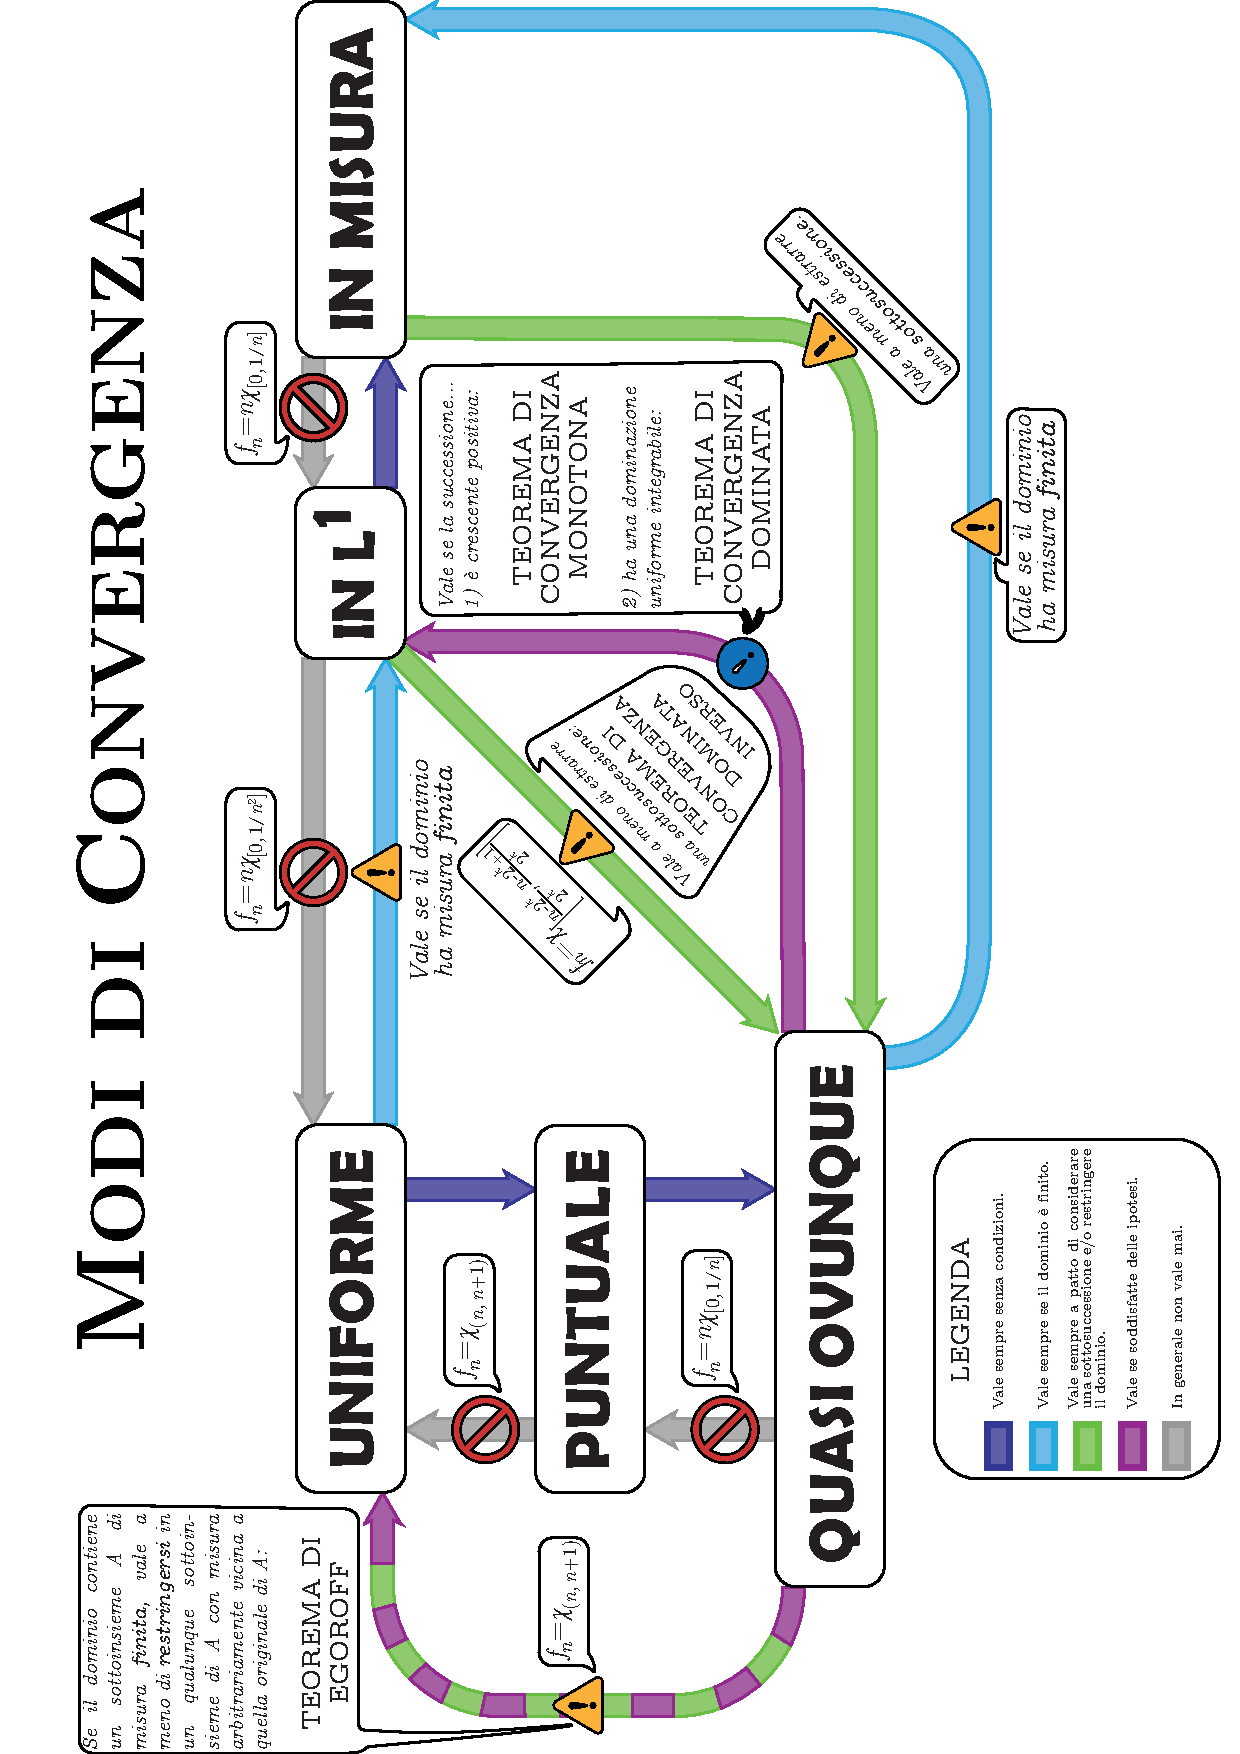
\includepdf{images/modiconvergenza2}
\newpage
\section{Passaggio al limite sotto segno di integrale}
	\begin{tabular}{p{0.49\textwidth}p{0.49\textwidth}}
		\multicolumn{2}{c}{\textbf{TEOREMA}} \\
		\begin{tabular}[c]{m{0.49\textwidth}}
		\centering \textbf{Convergenza uniforme} \\ \centering \textbf{(teoria di Riemann)}
		\end{tabular} &
		\begin{tabular}[c]{m{0.49\textwidth}}
		\centering \textbf{Convergenza uniforme} \\ \centering \textbf{(teoria di Lebesgue)}
		\end{tabular} \\
		Siano $\funz{f_n,f}{\left[a,b\right]}{\realset},\ n\geq 1$ tali che	\begin{enumerate}[label=(\alph*)]
			\item $f_n\in\mathcal{R}\left(\left[a,b\right]\right),\ \forall n\geq 1$.
			\item $f_n$ converge uniformemente a $f$ su $\left[a,b\right]$.
		\end{enumerate}
		Allora
		\begin{enumerate}
			\item $f\in\mathcal{R}\left(\left[a,b\right]\right)$.
			\item 
			Vale il \textbf{passaggio al limite sotto segno di integrale}:
			\begin{tabular}[c]{c}
			$\displaystyle\lim_{n\to+\infty}\int_{a}^{b}\!\!\! f_n(x)dx=\int_{a}^{b}\!\!\!\lim_{n\to+\infty}f_n(x)dx$
			\end{tabular}
		\end{enumerate} &
		Consideriamo lo spazio di misura $\left(X,\mathcal{M},\mu\right)$ e le funzioni $\funz{f_n,f}{X}{\complexset}$ tali che
		\begin{enumerate}[label=(\alph*)]
			\item $f_n\in L^{1}\left(\mu\right)$.
			\item $f_n$ converge uniformemente a $f$ su $X$.
			\item $\mu(X)<+\infty$.
		\end{enumerate}
			Allora
		\begin{enumerate}
			\item $f\in L^{1}\left(\mu\right)$.
			\item $\displaystyle\lim_{n\to+\infty}\norm{f_n-f}_1=0$.
			\item Vale il \textbf{passaggio al limite sotto segno di integrale}:
			\begin{tabular}[c]{c}
			$\displaystyle\lim_{n\to+\infty}\int_X\!\!\! f_nd\mu=\int_X\!\!\lim_{n\to+\infty}f_nd\mu$
			\end{tabular}
		\end{enumerate} \\
		\multicolumn{2}{c}{\textbf{VANTAGGI}} \\
		\begin{itemize}
			\item È l'unico teorema di questo tipo valido nella teoria di Riemann.
		\end{itemize} &
		\begin{itemize}
			\item Vale su spazi di misura finita invece che solamente degli intervalli finiti.
		\end{itemize} \\
		\multicolumn{2}{c}{\textbf{SVANTAGGI}} \\
		\begin{itemize}
			\item Richiede la convergenza uniforme.
			\item Vale solo per funzioni limitate.
			\item Vale solo su intervalli limitati.
		\end{itemize} &
		\begin{itemize}
			\item Richiede la convergenza uniforme.
			\item Richiede l'integrabilità della successione.
			\item Vale solo su spazi di misura finita.
		\end{itemize}
		\begin{comment} \\
		\multicolumn{1}{l}{
			\begin{tabular}[c]{p{3cm}}
				Siano $\funz{f_n,f}{\left[a,b\right]}{\realset},\ n\geq 1$ tali che	\begin{enumerate}
					\item $f_n\in\mathcal{R}\left(\left[a,b\right]\right),\ \forall n\geq 1$.
					\item $f_n$ converge uniformemente a $f$ su $\left[a,b\right]$.
				\end{enumerate}
				Allora
				\begin{enumerate}
					\item $f\in\mathcal{R}\left(\left[a,b\right]\right)$.
					\item Vale il \textbf{passaggio al limite sotto segno di integrale}:\\
					$\displaystyle	\lim_{n\to+\infty}\int_{a}^{b}f_n(x)dx=\int_{a}^{b}\lim_{n\to+\infty}f_n(x)dx=\int_{a}^{b}f(x)dx$
				\end{enumerate}
		\end{tabular}} &
		\multicolumn{1}{l}{
			\begin{tabular}[c]{p{3cm}}
				Siano $\left(X,\mathcal{M},\mu\right)$ uno spazio di misura e $\funz{f_n,f}{X}{\left[0,+\infty\right]}$ con $n\geq 1$ tali che	\begin{enumerate}
					\item $f_n$ sono misurabili.
					\item $\displaystyle\lim_{n\to+\infty}f_n(x)=f(x),\ \forall x\in X$.
					\item $0\leq f_n(x)\leq f_{n+1}(x),\ \forall n\geq 1,\ \forall x\in X$.
				\end{enumerate}
				allora
				\begin{enumerate}
					\item $f$ è misurabile.
					\item Vale il \textbf{passaggio al limite sotto segno di integrale}:\\
					$\displaystyle	\lim_{n\to+\infty}\int_Xf_nd\mu=\int_Xfd\mu\in\left[0,+\infty\right]$
				\end{enumerate}
		\end{tabular}}&
		\begin{tabular}[c]{p{3cm}}
			Sia $\left(X,\mathcal{M},\mu\right)$ uno spazio di misura e $\funz{f_n}{X}{\complexset}$ una successione di funzioni misurabili tale che esiste\\
			$\displaystyle f(x)=\lim_{n\to+\infty}f_n(x),\ \forall x\in X$
			Se esiste una funzione $g\in \mathcal{L}^{1}\left(\mu\right)$ tale per cui\\
			$\displaystyle\abs{f_n(x)}\leq g(x),\ \forall n\geq 1,\ \forall x\in X$
			allora $f\in \mathcal{L}^{1}\left(\mu\right)$ e vale\\
			$\displaystyle \lim_{n\to+\infty}\int_X\abs{f_n-f}d\mu=0$
			e vale il \textbf{passaggio al limite sotto segno di integrale}:
			$\displaystyle \lim_{n\to+\infty}\int_Xf_nd\mu=\int_Xfd\mu$
		\end{tabular} &
		\begin{tabular}[c]{@{}l@{}}
			Consideriamo lo spazio di misura $\left(X,\mathcal{M},\mu\right)$ e le funzioni $\funz{f_n,f}{X}{\complexset}$. Se
			\begin{enumerate}[label=(\alph*)]
				\item $f_n\in L^{1}\left(\mu\right)$.
				\item $f_n$ converge uniformemente a $f$ su $X$.
				\item $\mu(X)<+\infty$.
			\end{enumerate}
			allora
			\begin{enumerate}
				\item $f\in L^{1}\left(\mu\right)$.
				\item $\displaystyle\lim_{n\to+\infty}\norm{f_n-f}_1=0$.
				\item Vale il \textbf{passaggio al limite sotto segno di integrale}\\
				$\displaystyle \lim_{n\to+\infty}\int_Xf_nd\mu=\int_Xfd\mu$
			\end{enumerate}
		\end{tabular} \\
		\multicolumn{4}{c}{\textbf{VANTAGGI}} \\
		\multicolumn{1}{l}{
			\begin{tabular}[c]{p{3cm}}
				\begin{enumerate}
					\item È l'unico teorema di questo tipo valido nella teoria di Riemann.
				\end{enumerate}
		\end{tabular}} &
		\begin{tabular}[c]{p{3cm}}
			\begin{enumerate}
				\item Richiede la convergenza puntuale.
				\item Si può applicare anche con la convergenza \textbf{q.o.} purché la misura sia completa o la funzione limite $f$ è una funzione misurabile che coincide \textbf{q.o.} con il limite \textbf{q.o.} della successione.
				\item È sufficiente anche solamente supporre che la successione $f_n$ sia non decrescente su $X$ \textbf{q.o.}.
				\item Vale qualunque sia la misura di $X$.
			\end{enumerate}
		\end{tabular} &
		\begin{tabular}[c]{p{3cm}}
			\begin{enumerate}
				\item Richiede la convergenza puntuale.
				\item Si può applicare anche con la convergenza \textbf{q.o.} e con la dominazione \textbf{q.o.} purché la misura sia completa o la funzione limite $f$ è una funzione misurabile che coincide \textbf{q.o.} con il limite \textbf{q.o.} della successione.
				\item Vale qualunque sia la misura di $X$.
				\item Vale per funzione a valori complessi.
			\end{enumerate}
		\end{tabular} &
		\begin{tabular}[c]{@{}l@{}}
			\begin{enumerate}
				\item Vale su spazi di misura finita invece che solamente degli intervalli finiti.
			\end{enumerate}
		\end{tabular} \\
		\multicolumn{4}{c}{\textit{\textbf{SVANTAGGI}}} \\
		\multicolumn{1}{l}{
			\begin{tabular}[c]{@{}l@{}}
				\begin{enumerate}
					\item Richiede la convergenza uniforme.
					\item Vale solo per funzioni limitate.
					\item Vale solo su intervalli limitati.
				\end{enumerate}
		\end{tabular}} &
		\begin{tabular}[c]{@{}l@{}}
			\begin{enumerate}
				\item Non vale per successioni decrescenti.
			\end{enumerate}
		\end{tabular} &
		\begin{tabular}[c]{@{}l@{}}
			\begin{enumerate}
				\item Richiede una dominazione della successione. \end{enumerate}
		\end{tabular} &
		\begin{tabular}[c]{@{}l@{}}
			\begin{enumerate}
				\item Richiede la convergenza uniforme.
				\item Richiede l'integrabilità della successione.
				\item Vale solo su spazi di misura finita.
			\end{enumerate}
		\end{tabular}
	\end{comment}
	\end{tabular}
% SVN info for this file
\svnidlong
{$HeadURL$}
{$LastChangedDate$}
{$LastChangedRevision$}
{$LastChangedBy$}

\chapter{Elenchi delle definizioni e dei teoremi}
\nocite{*}
\begin{multicols}{2}
	\listofdefines
\end{multicols}
\begin{center}
\rule{4cm}{0.4pt}
\end{center}
\begin{multicols}{2}
	\listoftheoremas
\end{multicols}
\begin{comment}
\end{comment}
% SVN info for this file
\svnidlong
{$HeadURL$}
{$LastChangedDate$}
{$LastChangedRevision$}
{$LastChangedBy$}

\chapter{Ringraziamenti}
\labelChapter{ringraziaments}

\begin{introduction}
  ‘‘Siete ancora qui? Il film è finito. Andatene via... 'ndate!''
	\begin{flushright}
		\textsc{Ferris Bueller,} Una pazza giornata di vacanza
	\end{flushright}
\end{introduction}

\section*{Titolari del corso di Geometria 2 - Università degli Studi di Torino}

\textit{Prof.} Alberto Albano.\\
\textit{Prof.ssa.} Cinzia Casagrande.\\
\textit{Prof.ssa.} Elena Martinengo.

\section*{Adattamento \LaTeX e integrazioni discutibili}
Elisa Antuca.\\
Massimo Bertolotti.

\section*{Ringraziamenti}
Al Frittellavenutamalfanclub, con cui condividiamo questo pazzo mondo universitario:
\begin{itemize}
	\item Alessandro Amatelli.
	\item Elisa Antuca.
	\item Massimo Bertolotti.
	\item Guido Buffa.
	\item Francesca Colombo.
	\item Samuele Corsato.
	\item Julian Kerpaci.
	\item Daniele Sciretti.
\end{itemize}
\backmatter
% SVN info for this file
\svnidlong
{$HeadURL$}
{$LastChangedDate$}
{$LastChangedRevision$}
{$LastChangedBy$}

\RaggedRight
\printbibliography
\printindex

\end{document}
